%*****************************************
\chapter{Numerical Evaluations}\label{ch:examples}

In Chapter 1, we covered the mathematical foundations of second-order optimization
and its application within the context of neural networks.
We discussed both fundamental and cutting-edge techniques for first-order and
second-order optimization, providing a comprehensive overview of the field.
In this chapter, we examine our experimental results, by comparing the performance and convergence properties of each
optimizer including second-order optimization methods, namely
AdaHessian\cite{yao2021adahessian} and Apollo\cite{apollo}, against established first-order optimizers on common datasets across multiple domains.
Our research will be conducted on two computer vision datasets,
namely CIFAR and (Tiny)ImageNet, as well as WMT-14, a machine translation dataset, which will
be used to train a transformer model.
For each of these datasets, we will discuss in depth the hyperparameter settings
 and model selection process used in our experiments, and relating them to our results.
This detailed documentation ensures that others can easily reproduce our results.
Furthermore, we provide a thorough comparison of our findings with those reported 
in the original papers of AdaHessian and Apollo. We critically analyze
these results, offering insights into the strengths and weaknesses of each method.

\section{Overview of Software and Tools Used}
To efficiently evaluate the optimizers across various datasets with a range of hyperparameters,
we developed a comprehensive benchmarking framework in Python 3.6.8.
The code for this framework is publicly accessible on our GitHub repository\footnote{\url{https://github.com/Neural-Opt/second_order_optim_models}}.
and is available for anyone to use and modify. The core of our framework is built on
\emph{PyTorch}. \emph{PyTorch} is a popular open-source machine learning framework known for its dynamic computation graph and easy to integrate GPU acceleration.
For datasets and pre-built computer vision model architectures, we utilized the PyTorch-associated \emph{torchvision} module.
Additionally, \emph{NumPy} is used in some of the utility functions and to prepare data for use with \emph{matplotlib}.
From the hardware side, most of the experiments, unless otherwise specified, were conducted on \emph{Nvidia A40} GPUs.
These GPUs are equipped with 48 \emph{GB} of GDDR6 memory and deliver FP32 performance of up to 19.5 TFLOPS.
For efficient multi-GPU training, we used the PyTorch \emph{DataParallel} module, which splits the input across the specified GPU's by chunking along the batch dimension\cite{pytorch_dataparallel}.
Because \emph{AdaHessian} uses \texttt{torch.autograd.grad} to compute the second order derivatives, we were not
able to utilize the more efficient \texttt{DDP} (Distributed Data Parallel) package, as DDP currently
doesn't work with the construction of derivative graphs. For more information on this, see this
issue\footnote{\url{https://github.com/pytorch/pytorch/issues/63812}}.

\section{Image Classification}

For evaluation, we choose the most widely used first-order optimizers, as well as AdaHessian and Apollo for second-order
optimizers. In addition to the regular metrics of \emph{Training Accuracy}, \emph{Training Loss},
\emph{Test Accuracy}, and \emph{Test Loss}, we also evaluate the speed of each optimization step and 
its memory usage during this step. This helps assess the real-world applicability of the second-order optimizers.
Finally, we introduced a new metric called \emph{Time till Convergence (TTC)}.
\emph{TTC} measures the time in epochs each optimizer needs for the \emph{Training Loss} to converge.
We compute the Time till Convergence (TTC) by following Algorithm \ref{alg:convergence},
which takes as input the loss data, a threshold, and a window size.
To prevent outliers from distorting the results, we rely on short-term intervals, from which we calculate the mean.
\begin{algorithm}
    \caption{Time till Convergence (TTC) Calculation}
    \label{alg:convergence}

    \begin{algorithmic}[1]
    \State \textbf{Input:} Loss array \texttt{data}, treshold \texttt{T}$=\frac{\texttt{data}[0]}{100}$, window size $\sigma=5$
    \State \textbf{Initialize:} $ \text{old\_mean} \gets mean(\texttt{data}[ \lvert \texttt{data}\rvert -\sigma :] )$ 
    \For{$i = n-\sigma, n-\sigma, \dots, 0$ }
    \State $ \text{new\_mean} \gets  mean(\texttt{data}[i:i+\sigma]) $
        \If{$ |\text{new\_mean} - \text{old\_mean}| \le \texttt{T} $}
            \State \textbf{continue}
        \Else
            \State $\texttt{ttc} \gets i + \arg\min (\text{new\_mean})$
            \State \textbf{break}
        \EndIf
    \EndFor
    \end{algorithmic}
    \end{algorithm}
For learning rate scheduling, we employ both \emph{milestone decay} as well as \emph{cosine annealing}.
While \emph{milestone decay} decays the learning rate by a factor of $\gamma$ at
specified milestones (certain epochs), \emph{cosine annealing} gradually reduces the learning rate
following a cosine function.
For our experiments, we use \emph{PyTorch's} implementation of \texttt{MultiStepLR} for milestone decay and
\texttt{CosineAnnealingLR} for cosine annealing.
In the next sections, we discuss the obtained results on the CIFAR-10 and TinyImageNet
datasets, as well as the chosen hyperparameters for the optimizers and learning rate schedulers.

\subsection{CIFAR-10}
\begin{figure}[h!]
    \centering
    \begin{tabular}{cc}
        % This file was created with tikzplotlib v0.10.1.
\begin{tikzpicture}[scale=0.75]

    \definecolor{crimson2143940}{RGB}{214,39,40}
    \definecolor{darkgrey176}{RGB}{176,176,176}
    \definecolor{darkorange25512714}{RGB}{255,127,14}
    \definecolor{forestgreen4416044}{RGB}{44,160,44}
    \definecolor{grey127}{RGB}{127,127,127}
    \definecolor{lightgrey204}{RGB}{204,204,204}
    \definecolor{mediumpurple148103189}{RGB}{148,103,189}
    \definecolor{orchid227119194}{RGB}{227,119,194}
    \definecolor{sienna1408675}{RGB}{140,86,75}
    \definecolor{steelblue31119180}{RGB}{31,119,180}
    
    \begin{groupplot}[group style={group size=2 by 2,
        horizontal sep=1cm,  % Adjust horizontal spacing
        vertical sep=2cm}]
    \nextgroupplot[
    tick align=outside,
    tick pos=left,
    title={Polynom. Training Accuracy (milestone)},
    x grid style={darkgrey176},
    xlabel={Epochs},
    xmin=-8.15, xmax=171.15,
    xtick style={color=black},
    y grid style={darkgrey176},
    ymin=-0.0499509672805615, ymax=1.04947646161264,
    ytick style={color=black}
    ]
    \addplot [semithick, steelblue31119180]
    table {%
    0 0.00585453264392308
    1 0.0356371780360188
    2 0.0724429073953655
    3 0.114026662767667
    4 0.160377181943682
    5 0.201675866443559
    6 0.23912086690041
    7 0.274290514626252
    8 0.305161485752314
    9 0.328210279229728
    10 0.35117462457902
    11 0.376259712122904
    12 0.397675701775899
    13 0.414922358304259
    14 0.431427166280377
    15 0.450881603752108
    16 0.463317044115045
    17 0.485162655333872
    18 0.492813140803741
    19 0.515905744686257
    20 0.530875726128821
    21 0.546498020020407
    22 0.564215268987451
    23 0.566659257353538
    24 0.574840493291048
    25 0.596982730426941
    26 0.607763702338499
    27 0.613380548936622
    28 0.631255217888123
    29 0.631599686089729
    30 0.649015834427843
    31 0.658935377170777
    32 0.667984336441862
    33 0.6764042007152
    34 0.680783033441433
    35 0.688592836135743
    36 0.695357139461492
    37 0.706497755809059
    38 0.71635060021053
    39 0.719404256356127
    40 0.737262993112153
    41 0.738628764286434
    42 0.734148816123116
    43 0.740681215457724
    44 0.754183271719225
    45 0.767780816651133
    46 0.768082957745844
    47 0.782697997175586
    48 0.781369520100139
    49 0.782800262514264
    50 0.7956678797324
    51 0.791635158495066
    52 0.809439208887422
    53 0.801070389089789
    54 0.819998437916681
    55 0.812174082606553
    56 0.820954146947984
    57 0.817877826562029
    58 0.831525882585642
    59 0.824039717259099
    60 0.833459662872224
    61 0.835397039215823
    62 0.843942620667794
    63 0.846661435650293
    64 0.847641922564672
    65 0.854969690974223
    66 0.862127065611981
    67 0.858047015966618
    68 0.859809461743872
    69 0.86755424677148
    70 0.868331784328754
    71 0.860802109433728
    72 0.872450892295504
    73 0.887725936944379
    74 0.879612730750179
    75 0.884112709743086
    76 0.880736003744087
    77 0.886030768754388
    78 0.88490209604075
    79 0.89225907328608
    80 0.926734130320239
    81 0.958172142163436
    82 0.966254170774487
    83 0.971226724719804
    84 0.976830034647409
    85 0.97731849850135
    86 0.982459176579853
    87 0.981723472571698
    88 0.9845460668212
    89 0.984054715082111
    90 0.987128884564491
    91 0.987252010953173
    92 0.987498300589206
    93 0.98910038160839
    94 0.988360701427909
    95 0.988977070834394
    96 0.989840504578549
    97 0.990951519699253
    98 0.990087310667327
    99 0.990457612105862
    100 0.992310781623722
    101 0.993176542797388
    102 0.99218715075803
    103 0.991198547373383
    104 0.992434424813065
    105 0.991445624308958
    106 0.991692750513346
    107 0.993424014089807
    108 0.991075027379098
    109 0.994166723963222
    110 0.991816332093646
    111 0.994042908146009
    112 0.991816332093646
    113 0.994414392610996
    114 0.995033780184654
    115 0.992805428332213
    116 0.994909877985751
    117 0.994166723963222
    118 0.995281621615173
    119 0.992310781623722
    120 0.99429055211791
    121 0.996273481242038
    122 0.996521569661856
    123 0.996645632403804
    124 0.997266131470862
    125 0.997266131470862
    126 0.995777452632888
    127 0.996769707501676
    128 0.997762753208669
    129 0.996893794956395
    130 0.996645632403804
    131 0.996645632403804
    132 0.997638579230178
    133 0.998135349333226
    134 0.996273481242038
    135 0.997390268362198
    136 0.99801113825927
    137 0.997886939551392
    138 0.997514417614995
    139 0.99801113825927
    140 0.997762753208669
    141 0.998135349333226
    142 0.99801113825927
    143 0.998632317308303
    144 0.998259572774184
    145 0.998135349333226
    146 0.997638579230178
    147 0.997390268362198
    148 0.999005173178685
    149 0.998259572774184
    150 0.999005173178685
    151 0.998632317308303
    152 0.997886939551392
    153 0.998135349333226
    154 0.998259572774184
    155 0.997886939551392
    156 0.998508056760799
    157 0.998508056760799
    158 0.999253805624734
    159 0.999253805624734
    160 0.998135349333226
    161 0.998259572774184
    162 0.998259572774184
    163 0.998259572774184
    };
    \addplot [semithick, darkorange25512714]
    table {%
    0 0.00355649485238808
    1 0.0240025924295576
    2 0.0586813226507053
    3 0.0948560082048658
    4 0.128555684543424
    5 0.169797520877831
    6 0.211001701143654
    7 0.241346858678765
    8 0.264575091065413
    9 0.293316243246204
    10 0.317883378499788
    11 0.337810649351477
    12 0.367073742200474
    13 0.375634072567152
    14 0.397913724035592
    15 0.404564445979567
    16 0.416278151450991
    17 0.436979812775139
    18 0.447667686720465
    19 0.455504907905834
    20 0.473557422550801
    21 0.476368943263324
    22 0.477125520987742
    23 0.504721457626182
    24 0.506018607950702
    25 0.518327970964791
    26 0.534935884695477
    27 0.548957433905282
    28 0.550036207901335
    29 0.548111013756756
    30 0.569190960043069
    31 0.572846127853537
    32 0.577000643022155
    33 0.583681801314582
    34 0.598466285188004
    35 0.601856504995377
    36 0.606261733354692
    37 0.614390921618958
    38 0.616331190730658
    39 0.624653443482755
    40 0.62944922474313
    41 0.637739063486921
    42 0.644538669392334
    43 0.648751785026246
    44 0.655112740880495
    45 0.65635536711816
    46 0.66322356167833
    47 0.663940424433728
    48 0.664568187709898
    49 0.675585683882321
    50 0.678864512465781
    51 0.685276453625223
    52 0.682064455336253
    53 0.685184514635656
    54 0.692107378845168
    55 0.70339413628451
    56 0.705838498591132
    57 0.700862932503429
    58 0.709706873018829
    59 0.712642986161592
    60 0.714352280175168
    61 0.715493630481782
    62 0.709139712520631
    63 0.727662588025507
    64 0.719595455062418
    65 0.727469676417889
    66 0.740192123282861
    67 0.729014115490942
    68 0.743817531152537
    69 0.735607273566029
    70 0.736288679791105
    71 0.751902857007916
    72 0.742542124163426
    73 0.747161498368377
    74 0.746570514297804
    75 0.759459209188601
    76 0.747555695625809
    77 0.756071262837257
    78 0.757265625080453
    79 0.75210093468253
    80 0.839715220018862
    81 0.886595536825042
    82 0.907119823382116
    83 0.914508257742701
    84 0.927670958700634
    85 0.931543387553144
    86 0.933661065508624
    87 0.941221799891684
    88 0.94157740733809
    89 0.949905476862599
    90 0.945734108479494
    91 0.95265466666363
    92 0.960458546064031
    93 0.955770107418319
    94 0.962507973620457
    95 0.958653128119388
    96 0.960458546064031
    97 0.962266683079274
    98 0.967586266809523
    99 0.96528629549021
    100 0.966980586607416
    101 0.970012023380183
    102 0.974025156250867
    103 0.970983687154153
    104 0.968798537714328
    105 0.969890620123342
    106 0.975975692873219
    107 0.976585875971703
    108 0.974756241676348
    109 0.97731849850135
    110 0.976097705086202
    111 0.976952132296705
    112 0.977562803694235
    113 0.978662781732667
    114 0.976219729501627
    115 0.978785062610857
    116 0.976585875971703
    117 0.976707949206047
    118 0.980253386773063
    119 0.981355785881978
    120 0.985283462419244
    121 0.988853772359191
    122 0.988237464432872
    123 0.988730486181861
    124 0.989717119992471
    125 0.991075027379098
    126 0.990828024332928
    127 0.988853772359191
    128 0.991816332093646
    129 0.99156918125209
    130 0.990828024332928
    131 0.992310781623722
    132 0.991816332093646
    133 0.991445624308958
    134 0.992805428332213
    135 0.993300272278086
    136 0.993176542797388
    137 0.99305282564679
    138 0.99305282564679
    139 0.993300272278086
    140 0.993300272278086
    141 0.993671534710002
    142 0.993300272278086
    143 0.994042908146009
    144 0.994042908146009
    145 0.994662110616046
    146 0.994042908146009
    147 0.992310781623722
    148 0.993547768233472
    149 0.994662110616046
    150 0.994785988129856
    151 0.994909877985751
    152 0.994662110616046
    153 0.994662110616046
    154 0.994042908146009
    155 0.9945382454434
    156 0.99429055211791
    157 0.995901441258672
    158 0.995281621615173
    159 0.995529512428791
    160 0.996149455562325
    161 0.995901441258672
    162 0.994909877985751
    163 0.997514417614995
    };
    \addplot [semithick, forestgreen4416044]
    table {%
    0 0.00371221413409805
    1 0.0230120645232661
    2 0.0572285713466521
    3 0.0936337986914042
    4 0.132459012394655
    5 0.175164261603476
    6 0.217457203853749
    7 0.251198946036875
    8 0.290251314639308
    9 0.315404497171626
    10 0.3373410041195
    11 0.359437706826822
    12 0.388014403202341
    13 0.410631954831275
    14 0.427315594953929
    15 0.443497546389907
    16 0.464730497931824
    17 0.475476043655474
    18 0.493802725104933
    19 0.512471548759755
    20 0.521054610606036
    21 0.542978063536198
    22 0.54450624377301
    23 0.565554474155539
    24 0.577241059953409
    25 0.581743573064677
    26 0.606178377784594
    27 0.610273598027747
    28 0.625764135669152
    29 0.638607586351395
    30 0.645677553833571
    31 0.657599878264387
    32 0.654935376591715
    33 0.675949371257549
    34 0.67631321524269
    35 0.684082016248567
    36 0.695729316582229
    37 0.707440406253711
    38 0.709328725716562
    39 0.720552058478078
    40 0.733857402428575
    41 0.746176732717722
    42 0.733760285097386
    43 0.749035417441998
    44 0.762158279631054
    45 0.772828933383486
    46 0.766975571889548
    47 0.775058499491976
    48 0.780961121039368
    49 0.796600837433481
    50 0.793908011315045
    51 0.793908011315045
    52 0.806606950684575
    53 0.814388411336047
    54 0.817242499435878
    55 0.829488565804738
    56 0.820316908643737
    57 0.819149666187465
    58 0.827669090154437
    59 0.84481188040677
    60 0.836043631320462
    61 0.847206038521462
    62 0.85124481587738
    63 0.838742076036413
    64 0.857936959143618
    65 0.85321518778801
    66 0.869332294536079
    67 0.869777261663233
    68 0.868887509539238
    69 0.866000842625476
    70 0.866555374164734
    71 0.875578433637665
    72 0.871224663339978
    73 0.878827121798185
    74 0.883549207371451
    75 0.869666002803669
    76 0.889763562567664
    77 0.900007892249288
    78 0.88999019617896
    79 0.890330233183209
    80 0.933661065508624
    81 0.958412611002802
    82 0.969647850076219
    83 0.971834531552624
    84 0.978662781732667
    85 0.978785062610857
    86 0.980865708343813
    87 0.984300366423927
    88 0.985898296200873
    89 0.983809112788409
    90 0.985037614811511
    91 0.987375149627771
    92 0.988730486181861
    93 0.989963901469861
    94 0.99021073217187
    95 0.989347040056443
    96 0.99132207968303
    97 0.991445624308958
    98 0.991939925993913
    99 0.991075027379098
    100 0.99021073217187
    101 0.99132207968303
    102 0.991939925993913
    103 0.991198547373383
    104 0.99255808032698
    105 0.993671534710002
    106 0.992063532215067
    107 0.992310781623722
    108 0.99305282564679
    109 0.993795313520321
    110 0.99156918125209
    111 0.994042908146009
    112 0.992310781623722
    113 0.994662110616046
    114 0.993300272278086
    115 0.993919104665349
    116 0.994785988129856
    117 0.995157694727487
    118 0.9945382454434
    119 0.993795313520321
    120 0.993176542797388
    121 0.995901441258672
    122 0.995405560848633
    123 0.997390268362198
    124 0.996521569661856
    125 0.997886939551392
    126 0.997886939551392
    127 0.996025442234843
    128 0.996273481242038
    129 0.997638579230178
    130 0.997762753208669
    131 0.997638579230178
    132 0.996521569661856
    133 0.997142006940065
    134 0.997886939551392
    135 0.998259572774184
    136 0.997142006940065
    137 0.99801113825927
    138 0.998259572774184
    139 0.998383808583067
    140 0.998383808583067
    141 0.998508056760799
    142 0.997017894768884
    143 0.99801113825927
    144 0.997762753208669
    145 0.997638579230178
    146 0.998880875516322
    147 0.998383808583067
    148 0.998756590226503
    149 0.998880875516322
    150 0.998756590226503
    151 0.998632317308303
    152 0.998508056760799
    153 0.997514417614995
    154 0.998756590226503
    155 0.997762753208669
    156 0.998259572774184
    157 0.998135349333226
    158 0.998135349333226
    159 0.998259572774184
    160 0.999502487572043
    161 0.999129483214514
    162 0.999253805624734
    163 0.998508056760799
    };
    \addplot [semithick, crimson2143940]
    table {%
    0 0.000709854674871763
    1 0.00851372601023282
    2 0.0206558548610318
    3 0.0409941412605018
    4 0.0697419118932194
    5 0.105408464753558
    6 0.139594850919386
    7 0.17237273422524
    8 0.205681531555835
    9 0.239596476775031
    10 0.266556272865531
    11 0.296501073418166
    12 0.318879284165009
    13 0.341692042672669
    14 0.366181812742061
    15 0.383890458958542
    16 0.404323246173646
    17 0.423610750305946
    18 0.439745254734188
    19 0.459230790711401
    20 0.476850290675214
    21 0.478365630547102
    22 0.504577494177612
    23 0.514295964308871
    24 0.536370352187809
    25 0.544353271096978
    26 0.546881721257858
    27 0.567923980111683
    28 0.576760306203173
    29 0.592467866095433
    30 0.613296411252057
    31 0.611783511073663
    32 0.63297906300077
    33 0.636264743502343
    34 0.650425550351346
    35 0.648663787659843
    36 0.668795478208717
    37 0.688315981509163
    38 0.689516328353328
    39 0.693962893540643
    40 0.704803517366889
    41 0.715493630481782
    42 0.721318073460659
    43 0.723523996141183
    44 0.739605553755893
    45 0.736093940793599
    46 0.751209913772191
    47 0.755474647109055
    48 0.754679745404338
    49 0.77060450116096
    50 0.766573202949539
    51 0.780552892763074
    52 0.796912017735459
    53 0.80535071687166
    54 0.801278762408058
    55 0.806921253947683
    56 0.811437044361957
    57 0.809334168761832
    58 0.821485481325133
    59 0.816713361815437
    60 0.820847913072127
    61 0.825532619714601
    62 0.836690623729749
    63 0.838634004644206
    64 0.844485824107913
    65 0.852886539345072
    66 0.849714822509696
    67 0.858487356209815
    68 0.855738193137939
    69 0.855408767429102
    70 0.858707594114302
    71 0.867998485712839
    72 0.881972929145439
    73 0.875690297194555
    74 0.876249786491884
    75 0.884112709743086
    76 0.875690297194555
    77 0.884450949145527
    78 0.894418790272433
    79 0.890556982254536
    80 0.931425851544972
    81 0.957571181230169
    82 0.962146055956741
    83 0.970254866364991
    84 0.974878131915244
    85 0.976952132296705
    86 0.978051560648462
    87 0.978785062610857
    88 0.980988209368807
    89 0.980008543786281
    90 0.986144315637737
    91 0.98466893541793
    92 0.982704509240213
    93 0.985652325867234
    94 0.986267343772176
    95 0.986144315637737
    96 0.986882668641202
    97 0.988114239731109
    98 0.987867827203724
    99 0.991075027379098
    100 0.989717119992471
    101 0.988114239731109
    102 0.988607212301484
    103 0.991198547373383
    104 0.991939925993913
    105 0.991075027379098
    106 0.987867827203724
    107 0.990334165984407
    108 0.990334165984407
    109 0.989840504578549
    110 0.991075027379098
    111 0.99218715075803
    112 0.992310781623722
    113 0.99218715075803
    114 0.992063532215067
    115 0.993795313520321
    116 0.992310781623722
    117 0.991939925993913
    118 0.992805428332213
    119 0.993671534710002
    120 0.994414392610996
    121 0.994166723963222
    122 0.992681748166389
    123 0.992434424813065
    124 0.994166723963222
    125 0.995529512428791
    126 0.994166723963222
    127 0.993795313520321
    128 0.994042908146009
    129 0.9945382454434
    130 0.993919104665349
    131 0.993919104665349
    132 0.995901441258672
    133 0.994785988129856
    134 0.994662110616046
    135 0.996273481242038
    136 0.995901441258672
    137 0.995777452632888
    138 0.994909877985751
    139 0.995405560848633
    140 0.994909877985751
    141 0.994785988129856
    142 0.995157694727487
    143 0.993795313520321
    144 0.995777452632888
    145 0.995405560848633
    146 0.993671534710002
    147 0.994662110616046
    148 0.99429055211791
    149 0.996149455562325
    150 0.994909877985751
    151 0.993671534710002
    152 0.995777452632888
    153 0.996025442234843
    154 0.994662110616046
    155 0.993919104665349
    156 0.995901441258672
    157 0.995529512428791
    158 0.995777452632888
    159 0.993424014089807
    160 0.994414392610996
    161 0.995033780184654
    162 0.9945382454434
    163 0.995777452632888
    };
    \addplot [semithick, mediumpurple148103189]
    table {%
    0 0.000616880690070461
    1 0.00813067721428345
    2 0.0231952515024481
    3 0.0417140359547222
    4 0.0662381647100413
    5 0.0949316358734989
    6 0.127115890764143
    7 0.156107837382671
    8 0.185592348618141
    9 0.218486898572676
    10 0.24718770430879
    11 0.275441580439721
    12 0.303049450369812
    13 0.331077442575934
    14 0.353388356740664
    15 0.366627560483218
    16 0.35420104234318
    17 0.404805760882321
    18 0.423047870690124
    19 0.440584068950806
    20 0.454378634577391
    21 0.479884820343294
    22 0.494298113031665
    23 0.510579652679579
    24 0.529453029720829
    25 0.535388542457076
    26 0.546498020020407
    27 0.561466069932077
    28 0.578444346994803
    29 0.59304096323392
    30 0.601773634328662
    31 0.613464695855163
    32 0.622947766375082
    33 0.634360848842886
    34 0.644538669392334
    35 0.660898032937532
    36 0.658935377170777
    37 0.678225967551678
    38 0.677132437076221
    39 0.692849107829507
    40 0.702924843957625
    41 0.717017699754717
    42 0.727855540556248
    43 0.724580908653453
    44 0.743523051031461
    45 0.748936696481405
    46 0.750616369136115
    47 0.751704821069011
    48 0.764363191255788
    49 0.767780816651133
    50 0.779635003294701
    51 0.7957714985112
    52 0.797327076069024
    53 0.808704156984531
    54 0.81206875865159
    55 0.814493975903263
    56 0.812700866318208
    57 0.829809981638419
    58 0.831847929786498
    59 0.841230794742894
    60 0.848405151330755
    61 0.851354185393101
    62 0.848841528829664
    63 0.857936959143618
    64 0.869666002803669
    65 0.867443215461248
    66 0.862790155234974
    67 0.886369595048228
    68 0.889536975128031
    69 0.887499764732319
    70 0.88965026307683
    71 0.885466288529639
    72 0.890443601944768
    73 0.897723261524546
    74 0.898864996206126
    75 0.907234899220931
    76 0.906199636986631
    77 0.899207743035815
    78 0.910808047111126
    79 0.910000224911495
    80 0.936136555555043
    81 0.957811529408279
    82 0.967465106495774
    83 0.970376306094784
    84 0.975975692873219
    85 0.976830034647409
    86 0.976219729501627
    87 0.980743219556991
    88 0.978173780427457
    89 0.985283462419244
    90 0.981478335868823
    91 0.981478335868823
    92 0.983686330032305
    93 0.986636501850549
    94 0.984791816281279
    95 0.985529359111827
    96 0.988853772359191
    97 0.988114239731109
    98 0.986021299780942
    99 0.986390384185179
    100 0.986882668641202
    101 0.989840504578549
    102 0.988237464432872
    103 0.989470387732338
    104 0.989840504578549
    105 0.990951519699253
    106 0.991075027379098
    107 0.989470387732338
    108 0.989470387732338
    109 0.99156918125209
    110 0.99156918125209
    111 0.989963901469861
    112 0.99156918125209
    113 0.991939925993913
    114 0.99132207968303
    115 0.99218715075803
    116 0.99255808032698
    117 0.99218715075803
    118 0.994166723963222
    119 0.992434424813065
    120 0.992681748166389
    121 0.99305282564679
    122 0.992434424813065
    123 0.992310781623722
    124 0.994042908146009
    125 0.993671534710002
    126 0.9945382454434
    127 0.994414392610996
    128 0.993176542797388
    129 0.993795313520321
    130 0.993300272278086
    131 0.994042908146009
    132 0.994662110616046
    133 0.992681748166389
    134 0.993424014089807
    135 0.993176542797388
    136 0.994042908146009
    137 0.99429055211791
    138 0.993795313520321
    139 0.99429055211791
    140 0.995281621615173
    141 0.992434424813065
    142 0.995281621615173
    143 0.99429055211791
    144 0.994166723963222
    145 0.99156918125209
    146 0.995777452632888
    147 0.994414392610996
    148 0.994042908146009
    149 0.993795313520321
    150 0.992681748166389
    151 0.995901441258672
    152 0.995033780184654
    153 0.99305282564679
    154 0.995281621615173
    155 0.99305282564679
    156 0.993176542797388
    157 0.993919104665349
    158 0.993424014089807
    159 0.993424014089807
    160 0.992929120825373
    161 0.994785988129856
    162 0.99429055211791
    163 0.995033780184654
    };
    \addplot [semithick, sienna1408675]
    table {%
    0 2.30067600387449e-05
    1 3.56277958117278e-05
    2 4.8864932145611e-05
    3 7.1762493500528e-05
    4 8.7561021046252e-05
    5 0.000103582220061996
    6 0.000124557097014105
    7 0.000159904719152685
    8 0.000169856246786421
    9 0.000247046225728759
    10 0.000289138643202528
    11 0.000383557016859859
    12 0.000525869054429933
    13 0.000634922892774397
    14 0.000792933052366958
    15 0.000890814667788844
    16 0.00100955816813831
    17 0.00110049938046144
    18 0.00122676472900716
    19 0.0013485612455668
    20 0.00147443180424915
    21 0.00158289264500442
    22 0.001693111309805
    23 0.00182055594048963
    24 0.00201123588907528
    25 0.00222977029471024
    26 0.00228678500150959
    27 0.002530785680105
    28 0.00297667474406297
    29 0.00311672931423055
    30 0.00337578974750509
    31 0.00354148741509701
    32 0.00371362863420893
    33 0.00416099176208333
    34 0.00420299649784146
    35 0.0047667813649394
    36 0.00472375083352132
    37 0.00522573211295075
    38 0.00534581573482624
    39 0.00553396275023762
    40 0.0058667601514482
    41 0.00606310072862915
    42 0.00656251059208603
    43 0.00672926918126949
    44 0.00679324384551623
    45 0.0073422612454883
    46 0.00732275730845771
    47 0.00749234942073823
    48 0.00810423084972003
    49 0.0081731349663647
    50 0.00873580162101391
    51 0.00891392739162936
    52 0.009426994768444
    53 0.00946281838196631
    54 0.00993851892212506
    55 0.0105729090848007
    56 0.0104460980747692
    57 0.0112908481112071
    58 0.0111879177656998
    59 0.0119424537797259
    60 0.0123217575858721
    61 0.0121491661057162
    62 0.0125037761745771
    63 0.0127903405622808
    64 0.0132769918471296
    65 0.0136977698068196
    66 0.0140469361976131
    67 0.0139651064297552
    68 0.0143030493289072
    69 0.0148436189513029
    70 0.0147922569972932
    71 0.0160603333178171
    72 0.0157928031201358
    73 0.0165828402113805
    74 0.01670496574435
    75 0.0173507005331872
    76 0.0174334108057802
    77 0.017901441495423
    78 0.0183896431185911
    79 0.018588906671973
    80 0.0198751516459469
    81 0.0184865056285126
    82 0.0193608621936538
    83 0.0187485246217449
    84 0.0191655128516268
    85 0.0197401820822548
    86 0.0185530148233886
    87 0.0188002475118965
    88 0.0196702882732228
    89 0.0192603497103331
    90 0.0191444888158594
    91 0.0197671171591351
    92 0.0196595529745248
    93 0.0192761922871056
    94 0.0196488223634742
    95 0.0199564870734811
    96 0.0202350215806896
    97 0.0201692059865206
    98 0.020312023476468
    99 0.0201473055531821
    100 0.0197617277930187
    101 0.0206056570412421
    102 0.0197294162764016
    103 0.0203175325687807
    104 0.0205000043376984
    105 0.0202679937450794
    106 0.0199619188881123
    107 0.0209817037206241
    108 0.0208351289021353
    109 0.0202844959374509
    110 0.0200598939792464
    111 0.0207621493231599
    112 0.0199890957055308
    113 0.0208914065661125
    114 0.0206168036692628
    115 0.0208857733335059
    116 0.0209591002175037
    117 0.0205611187307882
    118 0.0202844959374509
    119 0.0209930127828961
    120 0.0206837847813112
    121 0.0217793747799108
    122 0.0207117449058917
    123 0.0213804324022775
    124 0.0210496312644303
    125 0.0208182692745173
    126 0.0214378850278165
    127 0.0209026766778241
    128 0.0203285543394711
    129 0.0210836609462758
    130 0.0215589375797021
    131 0.021605196413835
    132 0.0210609696058125
    133 0.0206112297524387
    134 0.0208070355874952
    135 0.0214724158421765
    136 0.0210439639252611
    137 0.0214493903595044
    138 0.0211404748743682
    139 0.0207453369595503
    140 0.0205166574678819
    141 0.02106664060842
    142 0.0208745105138082
    143 0.0208857733335059
    144 0.0206726091900544
    145 0.0207397352592645
    146 0.0214839359963413
    147 0.0210496312644303
    148 0.0209986691423995
    149 0.0211917120652356
    150 0.0218493598596593
    151 0.0204889082598326
    152 0.0208182692745173
    153 0.0210723128325681
    154 0.0215416109590967
    155 0.0213804324022775
    156 0.02098735764237
    157 0.0224038240438797
    158 0.0212716117830396
    159 0.0212887644634048
    160 0.0203726892649642
    161 0.0211860141431172
    162 0.0212316318559743
    163 0.0211917120652356
    };
    \addplot [semithick, orchid227119194]
    table {%
    0 3.75949387703222e-05
    1 0.000146441923245283
    2 0.000502028086433914
    3 0.000936419622578579
    4 0.00128741929984854
    5 0.00197255943120109
    6 0.00280421194821624
    7 0.00391300821373321
    8 0.00474953168569596
    9 0.00556126779287594
    10 0.00641439373251906
    11 0.00756705815689785
    12 0.00852472139299781
    13 0.00951675792512447
    14 0.00990746301578644
    15 0.0112736406526426
    16 0.0119208593297474
    17 0.0126162734355402
    18 0.0136375863770914
    19 0.0143697456427609
    20 0.015255290740297
    21 0.0164102786901832
    22 0.0172441300222339
    23 0.0183998200099404
    24 0.0199782214289383
    25 0.0210552998245484
    26 0.0223919109185277
    27 0.0228058536896297
    28 0.0237768053426474
    29 0.024974905602243
    30 0.0268483814226197
    31 0.0283618811503504
    32 0.0295988324269152
    33 0.0307325250405312
    34 0.0318532942883388
    35 0.0324578548139198
    36 0.0352673403704687
    37 0.0351732257361253
    38 0.0367919182171786
    39 0.037353494021106
    40 0.0390516035792484
    41 0.0407243551548601
    42 0.0410714850265459
    43 0.0424936975251855
    44 0.044561036428665
    45 0.046451263589658
    46 0.047063020873781
    47 0.0492047981438456
    48 0.0487703263305135
    49 0.0506182471856837
    50 0.0527814088787669
    51 0.054107148716532
    52 0.0543730428770201
    53 0.0573422052388608
    54 0.0574054131309111
    55 0.0588746499243074
    56 0.0613145310858085
    57 0.0615415030150615
    58 0.06297194917967
    59 0.0643179832564655
    60 0.0654056830251742
    61 0.0670934279482112
    62 0.0693290994369117
    63 0.0694763074258233
    64 0.0697862581689537
    65 0.0731924791952697
    66 0.0748039721544324
    67 0.0754942436314038
    68 0.0763006973751309
    69 0.0791368466986102
    70 0.080735619085999
    71 0.0808519863469931
    72 0.0840964722767268
    73 0.0830885835741543
    74 0.0862991934519413
    75 0.0889061787415897
    76 0.088995946685344
    77 0.0915757896808854
    78 0.0938210063225176
    79 0.0935589993673036
    80 0.0971844483626812
    81 0.100267689788371
    82 0.0981906902878403
    83 0.0999322410542467
    84 0.100961156128272
    85 0.101658454065398
    86 0.100861855289977
    87 0.102500291626756
    88 0.101818376091519
    89 0.100267689788371
    90 0.101618504974028
    91 0.100643668467481
    92 0.10068331068712
    93 0.103266751094561
    94 0.102741838100523
    95 0.103327455770801
    96 0.100782470889292
    97 0.104037788762177
    98 0.103671988406203
    99 0.10068331068712
    100 0.1034489507669
    101 0.102399781444624
    102 0.104527128024826
    103 0.102118772334669
    104 0.104078496899865
    105 0.105264587687958
    106 0.104037788762177
    107 0.102621008009113
    108 0.103570560021606
    109 0.105861674338141
    110 0.105079833786574
    111 0.104119217779252
    112 0.104527128024826
    113 0.104629305072762
    114 0.107188972841775
    115 0.107481086197182
    116 0.107168131930957
    117 0.108235160082375
    118 0.107147294261969
    119 0.105511330372192
    120 0.105758535536217
    121 0.106420015263094
    122 0.105923596232994
    123 0.106212948323374
    124 0.10775290422818
    125 0.106627405026047
    126 0.106026863779871
    127 0.107690128234103
    128 0.108067223481568
    129 0.11148734034839
    130 0.108571659620752
    131 0.107773836063897
    132 0.109120255974715
    133 0.109607399199637
    134 0.107836651089427
    135 0.10821415659721
    136 0.105964893591545
    137 0.108046246071995
    138 0.10882458308528
    139 0.107773836063897
    140 0.107983333388205
    141 0.108676987183277
    142 0.109501350793171
    143 0.108592718597262
    144 0.109904771915115
    145 0.10924716949434
    146 0.109141400032932
    147 0.10909911519363
    148 0.107001521318508
    149 0.108508502293125
    150 0.108319206638412
    151 0.107251515028987
    152 0.110843576391221
    153 0.107836651089427
    154 0.109268333223353
    155 0.1088456812983
    156 0.108088204149261
    157 0.108655915134016
    158 0.106876699399548
    159 0.109162547368663
    160 0.10815116570486
    161 0.108382275812215
    162 0.1072098169948
    163 0.108193156372822
    };
    \addplot [semithick, grey127]
    table {%
    0 0.00104190346710356
    1 0.00657814199038433
    2 0.0197725077010063
    3 0.0416552920745195
    4 0.0692115127960219
    5 0.0972808423725182
    6 0.134196253664325
    7 0.165534615210903
    8 0.19613922729695
    9 0.224558920471218
    10 0.254886769520162
    11 0.277889262150183
    12 0.304728523471964
    13 0.328465465414467
    14 0.35133622782112
    15 0.3667390652149
    16 0.387081984894126
    17 0.400958511016918
    18 0.421425134319697
    19 0.433717924842102
    20 0.448453068433777
    21 0.469399010695922
    22 0.480299813965541
    23 0.495644741831933
    24 0.505369699844347
    25 0.523347916105072
    26 0.531025661374039
    27 0.544123876548574
    28 0.550730600556733
    29 0.565633330049749
    30 0.583439240658016
    31 0.587899020623724
    32 0.599539574519673
    33 0.608432198894125
    34 0.620226434804082
    35 0.626106204776055
    36 0.639825107815009
    37 0.64287703734365
    38 0.660808719978807
    39 0.665555632162924
    40 0.668975838898644
    41 0.680325849805314
    42 0.691458887209535
    43 0.694148663668485
    44 0.705179733605442
    45 0.701143816971006
    46 0.711789567030319
    47 0.727662588025507
    48 0.729400634816058
    49 0.735218125146682
    50 0.742150043424404
    51 0.746472053320638
    52 0.755971800715889
    53 0.762759113877607
    54 0.757863371952539
    55 0.776581606252639
    56 0.780246833600941
    57 0.777496619040721
    58 0.786386289489417
    59 0.786181020294637
    60 0.796912017735459
    61 0.795046393707965
    62 0.808074537605489
    63 0.811542302766844
    64 0.810805723265675
    65 0.819043619159205
    66 0.815127593217198
    67 0.818195638262207
    68 0.823613570649168
    69 0.825532619714601
    70 0.832277481263116
    71 0.83895825224497
    72 0.838634004644206
    73 0.837877816777024
    74 0.847097095533858
    75 0.843074076608184
    76 0.853763160325416
    77 0.852229546278818
    78 0.850042492883135
    79 0.864449664441996
    80 0.908501504416564
    81 0.943713309841301
    82 0.953133435709473
    83 0.961422547237039
    84 0.959736052769553
    85 0.969162455822654
    86 0.970740698244671
    87 0.970497757984052
    88 0.971226724719804
    89 0.976097705086202
    90 0.978173780427457
    91 0.976463814943462
    92 0.975000034347433
    93 0.980865708343813
    94 0.980130959163337
    95 0.980253386773063
    96 0.982459176579853
    97 0.982827193947831
    98 0.979763749726508
    99 0.982459176579853
    100 0.9845460668212
    101 0.983195321591444
    102 0.983318055315962
    103 0.984914709412167
    104 0.9845460668212
    105 0.987005770460808
    106 0.988237464432872
    107 0.98540640462947
    108 0.986882668641202
    109 0.987744639376262
    110 0.985652325867234
    111 0.988360701427909
    112 0.988977070834394
    113 0.988114239731109
    114 0.987005770460808
    115 0.987005770460808
    116 0.988977070834394
    117 0.987128884564491
    118 0.989347040056443
    119 0.989963901469861
    120 0.989963901469861
    121 0.989717119992471
    122 0.993671534710002
    123 0.993671534710002
    124 0.99305282564679
    125 0.99218715075803
    126 0.992805428332213
    127 0.993424014089807
    128 0.994166723963222
    129 0.994414392610996
    130 0.993176542797388
    131 0.9945382454434
    132 0.9945382454434
    133 0.995653476356568
    134 0.993547768233472
    135 0.995157694727487
    136 0.996645632403804
    137 0.995033780184654
    138 0.995653476356568
    139 0.995653476356568
    140 0.995405560848633
    141 0.996025442234843
    142 0.995157694727487
    143 0.993795313520321
    144 0.995529512428791
    145 0.994909877985751
    146 0.995653476356568
    147 0.995529512428791
    148 0.996645632403804
    149 0.996645632403804
    150 0.996149455562325
    151 0.996149455562325
    152 0.9945382454434
    153 0.996521569661856
    154 0.995777452632888
    155 0.996769707501676
    156 0.996769707501676
    157 0.996893794956395
    158 0.995281621615173
    159 0.996521569661856
    160 0.996521569661856
    161 0.996521569661856
    162 0.995777452632888
    163 0.996645632403804
    };
    
    \nextgroupplot[
    tick align=outside,
    tick pos=left,
    title={Polynom. Test Accuracy (milestone)},
    x grid style={darkgrey176},
    xlabel={Epochs},
    xmin=-8.15, xmax=171.15,
    xtick style={color=black},
    y grid style={darkgrey176},
    ymin=-0.0305966063720012, ymax=0.643226759570355,
    ytick style={color=black}
    ]
    \addplot [semithick, steelblue31119180]
    table {%
    0 0.0143995262976747
    1 0.0290272617848877
    2 0.0807148533247029
    3 0.0898378858409333
    4 0.145059579721419
    5 0.166900903261357
    6 0.237923312522558
    7 0.194043515466
    8 0.273990102412403
    9 0.276250734560735
    10 0.239942759709642
    11 0.233772516681854
    12 0.317411195817584
    13 0.23838812739612
    14 0.358154230990301
    15 0.268488472394943
    16 0.31956167030393
    17 0.33657504035122
    18 0.404869125121346
    19 0.401328430417409
    20 0.386955372801743
    21 0.409868036557539
    22 0.392469432384552
    23 0.428869542781753
    24 0.455554647824097
    25 0.438378475388319
    26 0.432603149459766
    27 0.42812592451876
    28 0.438630968455799
    29 0.404869125121346
    30 0.40321370451525
    31 0.466062963316104
    32 0.419526338444119
    33 0.45816377414576
    34 0.400388441533278
    35 0.444725793468157
    36 0.367045843123009
    37 0.418552394956363
    38 0.449598751575706
    39 0.462099865902645
    40 0.466858835677243
    41 0.424177361017466
    42 0.330892524437914
    43 0.4437053125
    44 0.481643591988766
    45 0.430111202467942
    46 0.44498120685073
    47 0.455034251890535
    48 0.4437053125
    49 0.432353436265397
    50 0.409628879114786
    51 0.445748151182328
    52 0.428869542781753
    53 0.45633613434171
    54 0.448055331297725
    55 0.404632304160866
    56 0.434855764549861
    57 0.458687031028315
    58 0.457118692979656
    59 0.439895179538866
    60 0.410346686553879
    61 0.427136038411924
    62 0.448312273217391
    63 0.503532944958332
    64 0.456075519765793
    65 0.427383338103309
    66 0.467655794924312
    67 0.447798507200787
    68 0.503815036236942
    69 0.460784841525592
    70 0.466858835677243
    71 0.450114169097583
    72 0.502124383278527
    73 0.537109545858732
    74 0.510908513120312
    75 0.457902324840689
    76 0.485740106077155
    77 0.494294573137247
    78 0.493739061198424
    79 0.461047606597183
    80 0.584428180828231
    81 0.591131000808037
    82 0.584110522296319
    83 0.595956271780447
    84 0.587931554977186
    85 0.58825087473664
    86 0.587612373901664
    87 0.591451709893807
    88 0.586337035535469
    89 0.593057343951948
    90 0.587931554977186
    91 0.591772558161125
    92 0.584428180828231
    93 0.585700197281782
    94 0.593057343951948
    95 0.596925096120781
    96 0.587293331464896
    97 0.609634881712767
    98 0.596279073350048
    99 0.597895180037523
    100 0.587931554977186
    101 0.5946664632138
    102 0.602764536267924
    103 0.592735938505377
    104 0.588570333225214
    105 0.600488237751068
    106 0.600163614427623
    107 0.58920966657053
    108 0.589529541517697
    109 0.59821882146116
    110 0.594344360273028
    111 0.591131000808037
    112 0.592093545655287
    113 0.598542603019638
    114 0.595311088045607
    115 0.599839131512188
    116 0.602764536267924
    117 0.590169708187189
    118 0.603090284496517
    119 0.598866524758463
    120 0.601462950625131
    121 0.605047732653145
    122 0.606682819075251
    123 0.608321438526111
    124 0.607993431719051
    125 0.609306308430702
    126 0.608649586883199
    127 0.607665566416219
    128 0.611938865788477
    129 0.608321438526111
    130 0.610621452142302
    131 0.61226857422144
    132 0.61226857422144
    133 0.611938865788477
    134 0.612598424754793
    135 0.61226857422144
    136 0.609306308430702
    137 0.608321438526111
    138 0.611609299409984
    139 0.607993431719051
    140 0.611938865788477
    141 0.609634881712767
    142 0.61095059263279
    143 0.607665566416219
    144 0.608321438526111
    145 0.609306308430702
    146 0.609306308430702
    147 0.61226857422144
    148 0.610621452142302
    149 0.61226857422144
    150 0.609634881712767
    151 0.61226857422144
    152 0.608977876836123
    153 0.606682819075251
    154 0.604394686051705
    155 0.607665566416219
    156 0.605701343624516
    157 0.605701343624516
    158 0.609963596728154
    159 0.605047732653145
    160 0.611279875040054
    161 0.606028360863207
    162 0.612598424754793
    163 0.606355519331539
    };
    \addplot [semithick, darkorange25512714]
    table {%
    0 0.00552132192129307
    1 0.0328059736908033
    2 0.0474052084019847
    3 0.031648748274405
    4 0.135327665816518
    5 0.157557593180717
    6 0.155784312511088
    7 0.195891787062428
    8 0.175465485856424
    9 0.213594182394445
    10 0.288862055829757
    11 0.277124171116894
    12 0.285801341164944
    13 0.297831108868214
    14 0.311412986067274
    15 0.317411195817584
    16 0.319365692344475
    17 0.314303914854819
    18 0.357939535977298
    19 0.31956167030393
    20 0.375443702300072
    21 0.370563266787126
    22 0.343579912354481
    23 0.340887942225007
    24 0.327480048822165
    25 0.413709772180361
    26 0.302867597351074
    27 0.390394343105387
    28 0.314110520869259
    29 0.361603385547953
    30 0.384448898436464
    31 0.425161759203745
    32 0.355798243155354
    33 0.426888853211134
    34 0.404869125121346
    35 0.446516152638936
    36 0.383767573764167
    37 0.38970460062212
    38 0.401563703262636
    39 0.467124367939556
    40 0.467390021008174
    41 0.439136303619287
    42 0.450114169097583
    43 0.439642104422143
    44 0.446516152638936
    45 0.460259670801163
    46 0.442941181833296
    47 0.445748151182328
    48 0.447798507200787
    49 0.445492385667387
    50 0.425408144083083
    51 0.416852346859612
    52 0.442178104292394
    53 0.458948838687605
    54 0.426641782461182
    55 0.426641782461182
    56 0.433352981408416
    57 0.491522005684375
    58 0.457379784298512
    59 0.484918581675032
    60 0.455294390376698
    61 0.500999805044349
    62 0.492629535666944
    63 0.478927971986405
    64 0.466328133406711
    65 0.438126098610103
    66 0.476494399932492
    67 0.415157827369066
    68 0.437369665609343
    69 0.464474474804001
    70 0.410825783625485
    71 0.466062963316104
    72 0.472728515246852
    73 0.486837203554439
    74 0.468187705464067
    75 0.475415992770654
    76 0.453735342451039
    77 0.455554647824097
    78 0.470053205113419
    79 0.402034579973607
    80 0.581257806513348
    81 0.579993515950482
    82 0.584745977547647
    83 0.59049
    84 0.58379300190684
    85 0.577156904913446
    86 0.58189077803834
    87 0.58189077803834
    88 0.582841269142445
    89 0.583475619614735
    90 0.587293331464896
    91 0.58825087473664
    92 0.58825087473664
    93 0.58825087473664
    94 0.576528056743834
    95 0.58379300190684
    96 0.586018547202122
    97 0.585063912499649
    98 0.594988705789528
    99 0.589529541517697
    100 0.581574223384734
    101 0.58315837537495
    102 0.588570333225214
    103 0.587293331464896
    104 0.585063912499649
    105 0.58315837537495
    106 0.585063912499649
    107 0.586974427621711
    108 0.586337035535469
    109 0.591131000808037
    110 0.587612373901664
    111 0.587931554977186
    112 0.592093545655287
    113 0.59049
    114 0.584745977547647
    115 0.585700197281782
    116 0.585063912499649
    117 0.585063912499649
    118 0.591131000808037
    119 0.585063912499649
    120 0.591772558161125
    121 0.591131000808037
    122 0.598542603019638
    123 0.595633610027442
    124 0.592735938505377
    125 0.597895180037523
    126 0.597248317412813
    127 0.596925096120781
    128 0.594988705789528
    129 0.598866524758463
    130 0.594988705789528
    131 0.600813001528084
    132 0.597248317412813
    133 0.595311088045607
    134 0.599839131512188
    135 0.601462950625131
    136 0.597248317412813
    137 0.603416173543536
    138 0.606682819075251
    139 0.602438928812115
    140 0.601462950625131
    141 0.600488237751068
    142 0.599190586723145
    143 0.597571678703235
    144 0.599514788959209
    145 0.600163614427623
    146 0.602764536267924
    147 0.598866524758463
    148 0.604721138829035
    149 0.597895180037523
    150 0.596279073350048
    151 0.598866524758463
    152 0.599190586723145
    153 0.596925096120781
    154 0.600813001528084
    155 0.596279073350048
    156 0.597248317412813
    157 0.597248317412813
    158 0.594988705789528
    159 0.599839131512188
    160 0.603090284496517
    161 0.602764536267924
    162 0.600163614427623
    163 0.599514788959209
    };
    \addplot [semithick, forestgreen4416044]
    table {%
    0 0.00544548073993045
    1 0.0385300720464477
    2 0.043138108603297
    3 0.0265288552999108
    4 0.136713396879918
    5 0.142884346959259
    6 0.0983851503415281
    7 0.229078442393367
    8 0.132978284319506
    9 0.234996293703241
    10 0.176073052746473
    11 0.238698407358516
    12 0.253650293422207
    13 0.336166575544581
    14 0.326481756525511
    15 0.313724018491014
    16 0.367922684202194
    17 0.324294082074735
    18 0.374552547462951
    19 0.396180262203062
    20 0.403922506117718
    21 0.413468822989359
    22 0.389015833384316
    23 0.438378475388319
    24 0.409150899144576
    25 0.388328040357416
    26 0.398981761434421
    27 0.449856401283309
    28 0.381955429329792
    29 0.436111265978953
    30 0.428869542781753
    31 0.40015371974261
    32 0.438630968455799
    33 0.476764307255311
    34 0.455034251890535
    35 0.437117753586536
    36 0.470053205113419
    37 0.458425342861336
    38 0.435608717903793
    39 0.474608469472703
    40 0.486837203554439
    41 0.464474474804001
    42 0.441416078788356
    43 0.480012746110181
    44 0.399215933139106
    45 0.477034336874151
    46 0.462099865902645
    47 0.434605011607306
    48 0.474608469472703
    49 0.46341789090431
    50 0.485466140993279
    51 0.468720099888742
    52 0.474608469472703
    53 0.470053205113419
    54 0.48986444647435
    55 0.466593424180028
    56 0.441416078788356
    57 0.48986444647435
    58 0.493739061198424
    59 0.472192481153878
    60 0.464474474804001
    61 0.492629535666944
    62 0.472996714783376
    63 0.503532944958332
    64 0.490416468557669
    65 0.456596868042102
    66 0.459210765880125
    67 0.504379598076537
    68 0.462890320500361
    69 0.457379784298512
    70 0.472192481153878
    71 0.493461492585476
    72 0.462890320500361
    73 0.459734979028565
    74 0.438378475388319
    75 0.462626715541086
    76 0.49931671651599
    77 0.482188191200383
    78 0.504097253928849
    79 0.532964745020853
    80 0.587612373901664
    81 0.600813001528084
    82 0.599514788959209
    83 0.599514788959209
    84 0.60211346208346
    85 0.598866524758463
    86 0.603742203454631
    87 0.601462950625131
    88 0.607665566416219
    89 0.607665566416219
    90 0.604394686051705
    91 0.603742203454631
    92 0.602438928812115
    93 0.607010260140094
    94 0.600813001528084
    95 0.607993431719051
    96 0.606355519331539
    97 0.604721138829035
    98 0.604068374275463
    99 0.608321438526111
    100 0.610292453522713
    101 0.598866524758463
    102 0.603416173543536
    103 0.601462950625131
    104 0.605374467569735
    105 0.605701343624516
    106 0.609306308430702
    107 0.60211346208346
    108 0.605701343624516
    109 0.606355519331539
    110 0.594988705789528
    111 0.602764536267924
    112 0.605047732653145
    113 0.60211346208346
    114 0.604068374275463
    115 0.590810430858527
    116 0.600163614427623
    117 0.597248317412813
    118 0.606682819075251
    119 0.593700573114823
    120 0.597895180037523
    121 0.600488237751068
    122 0.602764536267924
    123 0.605047732653145
    124 0.603416173543536
    125 0.603742203454631
    126 0.607010260140094
    127 0.607665566416219
    128 0.607993431719051
    129 0.608649586883199
    130 0.606355519331539
    131 0.61095059263279
    132 0.607993431719051
    133 0.607337842571827
    134 0.607337842571827
    135 0.607665566416219
    136 0.607337842571827
    137 0.607010260140094
    138 0.606028360863207
    139 0.609963596728154
    140 0.609634881712767
    141 0.607665566416219
    142 0.608977876836123
    143 0.610292453522713
    144 0.609306308430702
    145 0.608321438526111
    146 0.609634881712767
    147 0.608977876836123
    148 0.608321438526111
    149 0.608321438526111
    150 0.608321438526111
    151 0.608321438526111
    152 0.608977876836123
    153 0.609963596728154
    154 0.609634881712767
    155 0.611609299409984
    156 0.611609299409984
    157 0.609306308430702
    158 0.61226857422144
    159 0.607665566416219
    160 0.608321438526111
    161 0.609306308430702
    162 0.609963596728154
    163 0.607010260140094
    };
    \addplot [semithick, crimson2143940]
    table {%
    0 0.00615066216529952
    1 0.0139616371321855
    2 0.027014225012693
    3 0.0567056685882856
    4 0.0816317604542996
    5 0.108311325056559
    6 0.140328890928603
    7 0.16924563895082
    8 0.197887679282701
    9 0.223869626105778
    10 0.215160950819177
    11 0.252349358644596
    12 0.273816822565677
    13 0.274510468372312
    14 0.282588919626629
    15 0.314303914854819
    16 0.295798518007925
    17 0.295430151281542
    18 0.348174278183084
    19 0.335147148300964
    20 0.315660341570524
    21 0.3444116232029
    22 0.337802817647072
    23 0.350067897417174
    24 0.379025300028548
    25 0.384448898436464
    26 0.357724943935522
    27 0.388786460847428
    28 0.377231100648871
    29 0.360738616398357
    30 0.379924956162886
    31 0.37255363544576
    32 0.368581414071976
    33 0.3973456345656
    34 0.37499791310519
    35 0.441416078788356
    36 0.398513747689565
    37 0.397812550653377
    38 0.429862640753325
    39 0.399215933139106
    40 0.435859933997401
    41 0.425901256518903
    42 0.427630752325058
    43 0.436865957652216
    44 0.433352981408416
    45 0.420746316503446
    46 0.418795711072887
    47 0.443960256938511
    48 0.388786460847428
    49 0.429614193967253
    50 0.444470497382198
    51 0.43110659940937
    52 0.418795711072887
    53 0.424915488497195
    54 0.449598751575706
    55 0.433352981408416
    56 0.427878281116946
    57 0.453994886742641
    58 0.41636763488084
    59 0.384903652228076
    60 0.449598751575706
    61 0.428373682570295
    62 0.441923978951817
    63 0.466062963316104
    64 0.449341219934183
    65 0.452180568325931
    66 0.469252978528409
    67 0.459210765880125
    68 0.430111202467942
    69 0.467921689729198
    70 0.447285212313001
    71 0.416852346859612
    72 0.438630968455799
    73 0.429862640753325
    74 0.457640994905233
    75 0.421479664541448
    76 0.464474474804001
    77 0.437117753586536
    78 0.437369665609343
    79 0.466858835677243
    80 0.528552322481783
    81 0.537406586856808
    82 0.53090196235163
    83 0.534146353569081
    84 0.539191593876276
    85 0.538001063111539
    86 0.536812636222068
    87 0.537109545858732
    88 0.540085874297523
    89 0.545476507902619
    90 0.541280093564038
    91 0.541578978202561
    92 0.545175903640167
    93 0.541578978202561
    94 0.539191593876276
    95 0.540384231308414
    96 0.541578978202561
    97 0.541280093564038
    98 0.536812636222068
    99 0.544575092696105
    100 0.545175903640167
    101 0.545175903640167
    102 0.544575092696105
    103 0.540682720160669
    104 0.542476424390136
    105 0.546680251245057
    106 0.542775837355791
    107 0.540682720160669
    108 0.543974811567653
    109 0.546379116377826
    110 0.543375059904325
    111 0.542775837355791
    112 0.543674869574748
    113 0.547282919306046
    114 0.542775837355791
    115 0.53948955562512
    116 0.541280093564038
    117 0.545175903640167
    118 0.541877994857264
    119 0.543075382512598
    120 0.542775837355791
    121 0.543075382512598
    122 0.543674869574748
    123 0.542775837355791
    124 0.542775837355791
    125 0.545175903640167
    126 0.542775837355791
    127 0.543674869574748
    128 0.544274885926837
    129 0.543674869574748
    130 0.543075382512598
    131 0.542775837355791
    132 0.544875431919274
    133 0.542177143571877
    134 0.544274885926837
    135 0.542476424390136
    136 0.544575092696105
    137 0.545476507902619
    138 0.543974811567653
    139 0.543375059904325
    140 0.546379116377826
    141 0.545476507902619
    142 0.544575092696105
    143 0.547584452587599
    144 0.544274885926837
    145 0.544274885926837
    146 0.543674869574748
    147 0.543974811567653
    148 0.544875431919274
    149 0.545175903640167
    150 0.545175903640167
    151 0.543974811567653
    152 0.544274885926837
    153 0.547886118761737
    154 0.545476507902619
    155 0.546680251245057
    156 0.544875431919274
    157 0.544274885926837
    158 0.543375059904325
    159 0.543674869574748
    160 0.547282919306046
    161 0.543075382512598
    162 0.544274885926837
    163 0.544274885926837
    };
    \addplot [semithick, mediumpurple148103189]
    table {%
    0 0.00520837083036211
    1 0.0176656935747745
    2 0.0402187672607123
    3 0.0538170687035372
    4 0.0659567900652955
    5 0.107570934452744
    6 0.112669376249212
    7 0.126498380065565
    8 0.149276146999
    9 0.2097871484388
    10 0.241505492210045
    11 0.239164433002096
    12 0.27590197720773
    13 0.300434186751569
    14 0.268317981879493
    15 0.309115593037733
    16 0.249763502588184
    17 0.316632081819948
    18 0.309497547263983
    19 0.312759426863714
    20 0.348174278183084
    21 0.365952143534156
    22 0.32768
    23 0.357939535977298
    24 0.343995566688078
    25 0.38970460062212
    26 0.406054893770889
    27 0.389474903233349
    28 0.366389310063579
    29 0.372332061980255
    30 0.37611318091434
    31 0.382181572265625
    32 0.368361732701375
    33 0.309688665911523
    34 0.405580253385898
    35 0.384676221572513
    36 0.393163086209921
    37 0.360091125929277
    38 0.40274172317346
    39 0.381051927832095
    40 0.377455003242663
    41 0.348594372581802
    42 0.386726972753334
    43 0.399684606406478
    44 0.38764122050759
    45 0.415883373901779
    46 0.407719635742398
    47 0.376560030312544
    48 0.420257985176687
    49 0.386042419633683
    50 0.395249934418099
    51 0.376783614221638
    52 0.414433293815621
    53 0.430608670842294
    54 0.448312273217391
    55 0.427383338103309
    56 0.404158994697954
    57 0.446516152638936
    58 0.433853446745288
    59 0.446004034155597
    60 0.459734979028565
    61 0.437873838080977
    62 0.441923978951817
    63 0.467655794924312
    64 0.432852978021744
    65 0.444725793468157
    66 0.446772388229937
    67 0.461310491529677
    68 0.45633613434171
    69 0.473802043850091
    70 0.457118692979656
    71 0.453735342451039
    72 0.465003488957338
    73 0.449341219934183
    74 0.478115679140956
    75 0.470320189773754
    76 0.480827615907949
    77 0.453216609977071
    78 0.467655794924312
    79 0.443960256938511
    80 0.523586956796628
    81 0.522133679807484
    82 0.52913895097282
    83 0.532079911660473
    84 0.528845571654813
    85 0.528259203410425
    86 0.531785228508833
    87 0.52913895097282
    88 0.537703759259879
    89 0.531196253897808
    90 0.534146353569081
    91 0.537703759259879
    92 0.53621921085869
    93 0.530019870229887
    94 0.53385075515155
    95 0.535626310418194
    96 0.532374725434074
    97 0.53090196235163
    98 0.537109545858732
    99 0.539787649084315
    100 0.53621921085869
    101 0.536812636222068
    102 0.538298498455392
    103 0.537109545858732
    104 0.538893763794133
    105 0.537703759259879
    106 0.536812636222068
    107 0.537109545858732
    108 0.531490675935745
    109 0.531785228508833
    110 0.534146353569081
    111 0.532374725434074
    112 0.53503393455226
    113 0.536515857903242
    114 0.538001063111539
    115 0.541578978202561
    116 0.543075382512598
    117 0.542775837355791
    118 0.537406586856808
    119 0.536812636222068
    120 0.535330056935171
    121 0.541877994857264
    122 0.538893763794133
    123 0.541280093564038
    124 0.540085874297523
    125 0.539191593876276
    126 0.53948955562512
    127 0.537703759259879
    128 0.539787649084315
    129 0.540682720160669
    130 0.540384231308414
    131 0.541280093564038
    132 0.538596065335049
    133 0.53948955562512
    134 0.53948955562512
    135 0.538298498455392
    136 0.540384231308414
    137 0.538596065335049
    138 0.53948955562512
    139 0.538298498455392
    140 0.538893763794133
    141 0.53948955562512
    142 0.53948955562512
    143 0.539787649084315
    144 0.539787649084315
    145 0.538298498455392
    146 0.540384231308414
    147 0.540981340897977
    148 0.538893763794133
    149 0.538596065335049
    150 0.539191593876276
    151 0.542177143571877
    152 0.541877994857264
    153 0.538596065335049
    154 0.538893763794133
    155 0.535922695044855
    156 0.539191593876276
    157 0.53621921085869
    158 0.538893763794133
    159 0.537703759259879
    160 0.537406586856808
    161 0.538893763794133
    162 0.538001063111539
    163 0.538893763794133
    };
    \addplot [semithick, sienna1408675]
    table {%
    0 3.17284435604748e-05
    1 4.44524445413208e-05
    2 5.09191764656831e-05
    3 6.88058043405684e-05
    4 7.2539319813757e-05
    5 9.16861325084006e-05
    6 0.000113992217512587
    7 0.000156051624586896
    8 0.00021025765522191
    9 0.000279277990102795
    10 0.000366208899516787
    11 0.000487613980972647
    12 0.000629817106061165
    13 0.000974656640901344
    14 0.00112610547489747
    15 0.00126268221785905
    16 0.00135921096731959
    17 0.00147211911084577
    18 0.00173851461814363
    19 0.0017936622798247
    20 0.00209781160515195
    21 0.002205443189485
    22 0.00244983986850044
    23 0.00268531462695381
    24 0.0029064677748736
    25 0.00332585213909132
    26 0.00332077140044529
    27 0.00378102873208444
    28 0.00417382957910325
    29 0.00431595176490443
    30 0.00498661867524019
    31 0.0052156532269174
    32 0.00555955807649347
    33 0.00599431153386831
    34 0.00631025840527096
    35 0.00668369901043735
    36 0.00699131899006275
    37 0.00717749548961985
    38 0.00713058391523891
    39 0.00783029045654919
    40 0.00800325017403053
    41 0.00811678427843443
    42 0.00867106761595946
    43 0.00926676105639909
    44 0.00938273909964829
    45 0.00911770713401267
    46 0.0095588807207605
    47 0.0099679382773712
    48 0.0105435362847857
    49 0.0107368722610775
    50 0.010985825030387
    51 0.0113746892209161
    52 0.0115387839724257
    53 0.0120424636328218
    54 0.0125635806241752
    55 0.0129510404317382
    56 0.0131178158554155
    57 0.0136441961801955
    58 0.0143667180946427
    59 0.0139616371321855
    60 0.0149157652759552
    61 0.0154120015256456
    62 0.0156386960009633
    63 0.0157442198824044
    64 0.0164623611894911
    65 0.0166828360984859
    66 0.0168870072283879
    67 0.0165172600775557
    68 0.0169617449173685
    69 0.0172064719295502
    70 0.0176463656843126
    71 0.0184728437752511
    72 0.0199828424180759
    73 0.0196016633251982
    74 0.0206532030887173
    75 0.0202833954569962
    76 0.0216582022676698
    77 0.0212516142982224
    78 0.0209396203467202
    79 0.0217037601023549
    80 0.0232266622769185
    81 0.0236875906412665
    82 0.0232748403609063
    83 0.0233956354114413
    84 0.023614330107802
    85 0.0243551531395789
    86 0.0239331066872071
    87 0.0235655905370039
    88 0.0235169314775555
    89 0.0231545447722547
    90 0.0240318812400014
    91 0.0233956354114413
    92 0.0238100955031166
    93 0.0243301632451738
    94 0.0244804108115395
    95 0.0232989593643907
    96 0.0244302460521555
    97 0.0235412509495996
    98 0.0241309816466586
    99 0.0239577698206109
    100 0.0238100955031166
    101 0.0246313997293408
    102 0.0248084941085786
    103 0.0248084941085786
    104 0.024910147297903
    105 0.0243551531395789
    106 0.0237610328874006
    107 0.0243301632451738
    108 0.0245558124304122
    109 0.0237610328874006
    110 0.0246061833107668
    111 0.0245306579432498
    112 0.0248338762367064
    113 0.0247831327386815
    114 0.0245809875486884
    115 0.024961098696899
    116 0.0244051945304205
    117 0.0251914127887846
    118 0.025631088015787
    119 0.0250632516141096
    120 0.0250121334349032
    121 0.0252943187496831
    122 0.025631088015787
    123 0.024180654296875
    124 0.025320097710801
    125 0.0250376820879658
    126 0.0245809875486884
    127 0.024961098696899
    128 0.0253975607297104
    129 0.0248847028186205
    130 0.0250121334349032
    131 0.0243551531395789
    132 0.0255270869843914
    133 0.0244051945304205
    134 0.0249866056421399
    135 0.0240071570844417
    136 0.0257615656935197
    137 0.0248847028186205
    138 0.0242802449951874
    139 0.02524282381818
    140 0.0253975607297104
    141 0.0259714347727075
    142 0.0251400855589274
    143 0.025631088015787
    144 0.0257354277434681
    145 0.025423423824032
    146 0.02586632995411
    147 0.0248338762367064
    148 0.0258925741990623
    149 0.0256571411626647
    150 0.0245306579432498
    151 0.0259714347727075
    152 0.0248084941085786
    153 0.0253458976859475
    154 0.0257093110135897
    155 0.0250376820879658
    156 0.0253975607297104
    157 0.0250888420261219
    158 0.0254493079837926
    159 0.0255530555346173
    160 0.025631088015787
    161 0.0246313997293408
    162 0.0246818945867753
    163 0.0259188397418383
    };
    \addplot [semithick, orchid227119194]
    table {%
    0 9.31322574615479e-05
    1 0.00055812204927284
    2 0.00113253300085813
    3 0.00167883909904391
    4 0.00245382334711954
    5 0.00342357389784187
    6 0.00453962870228823
    7 0.00562117629475368
    8 0.00810641006675626
    9 0.00906089208713485
    10 0.0104669862485315
    11 0.0110653936862946
    12 0.0120424636328218
    13 0.0116769714259058
    14 0.0130417971922825
    15 0.0156738075629335
    16 0.0140097585380435
    17 0.0164623611894911
    18 0.0162442234455906
    19 0.0168125332222356
    20 0.0165355922179006
    21 0.0197492020603862
    22 0.0203699285883374
    23 0.0211620962524414
    24 0.0216582022676698
    25 0.0250376820879658
    26 0.0257093110135897
    27 0.025423423824032
    28 0.0270958060636278
    29 0.0275618298345216
    30 0.0288837048865389
    31 0.0310673231820728
    32 0.0321450922129412
    33 0.0296657094079058
    34 0.035694649816254
    35 0.0361380985484979
    36 0.0351548540993284
    37 0.0376363906060831
    38 0.0350543734464396
    39 0.0391839712079848
    40 0.0387108283063769
    41 0.040782046539789
    42 0.0418503805794767
    43 0.0399580426624176
    44 0.043813742992932
    45 0.0428230607752267
    46 0.0425879850720848
    47 0.0452314155164073
    48 0.0492651990217567
    49 0.0483929619019068
    50 0.0490897533346197
    51 0.0517288739830106
    52 0.0508668966199189
    53 0.0553426153319094
    54 0.0583967717131243
    55 0.0564603173271305
    56 0.0582961916961722
    57 0.0562158160607255
    58 0.0624821713916121
    59 0.058952446330624
    60 0.063498033409104
    61 0.063068704129897
    62 0.0678645515949791
    63 0.0678645515949791
    64 0.064363706151411
    65 0.0677511226522824
    66 0.0701069597279439
    67 0.0694107690239932
    68 0.0724680477446003
    69 0.0701069597279439
    70 0.0786499841860493
    71 0.0735510780703735
    72 0.07776
    73 0.0778233018527183
    74 0.0783312022445376
    75 0.0811722711726023
    76 0.0800649786625911
    77 0.0857930622420926
    78 0.0844325909050303
    79 0.0866177251493979
    80 0.0941075438950851
    81 0.0943289038659712
    82 0.0960398724765135
    83 0.0960398724765135
    84 0.0949954842328182
    85 0.0966407770448443
    86 0.0955165364139293
    87 0.09506978071302
    88 0.0935926531452444
    89 0.0932262557988224
    90 0.0942550709767719
    91 0.0949212342096916
    92 0.0955165364139293
    93 0.0943289038659712
    94 0.0965654999204073
    95 0.0943289038659712
    96 0.0954419607332969
    97 0.0956658276264352
    98 0.0970934262618476
    99 0.0949212342096916
    100 0.0958153054529294
    101 0.0963399499568631
    102 0.0989210159051618
    103 0.0942550709767719
    104 0.096415086398347
    105 0.0956658276264352
    106 0.0946987626648931
    107 0.0952929491140824
    108 0.0933726767779582
    109 0.0934459562255951
    110 0.0938865996886022
    111 0.0968668901350895
    112 0.096415086398347
    113 0.0960398724765135
    114 0.0983851503415281
    115 0.0951441236720942
    116 0.0955911587043604
    117 0.0980038130087071
    118 0.0988443210601112
    119 0.0983087880739107
    120 0.0991513861264837
    121 0.0974719281659855
    122 0.0964902697122195
    123 0.0984615600538579
    124 0.0974719281659855
    125 0.0975477699987328
    126 0.0989977583498042
    127 0.098079985718387
    128 0.0983851503415281
    129 0.0970178671789248
    130 0.0986145219010822
    131 0.0977755787971616
    132 0.0972446856596122
    133 0.0971690324147473
    134 0.0986910740802073
    135 0.0971690324147473
    136 0.0973203860184376
    137 0.0957405432020053
    138 0.0981562057844281
    139 0.0976995952922879
    140 0.0976995952922879
    141 0.0970934262618476
    142 0.0982324732289078
    143 0.0978516095701547
    144 0.0976995952922879
    145 0.0985380172330054
    146 0.0977755787971616
    147 0.0990745484161915
    148 0.0976236590334905
    149 0.0977755787971616
    150 0.0983851503415281
    151 0.0976995952922879
    152 0.0990745484161915
    153 0.0976236590334905
    154 0.0979276876333176
    155 0.0983087880739107
    156 0.0961898176033873
    157 0.0971690324147473
    158 0.0967161011074708
    159 0.0966407770448443
    160 0.0970934262618476
    161 0.0964902697122195
    162 0.0970934262618476
    163 0.0967914721302345
    };
    \addplot [semithick, grey127]
    table {%
    0 0.00143540976044168
    1 0.000525972720053758
    2 0.00271111822931402
    3 0.020543880853526
    4 0.00792148074368431
    5 0.0201112114330102
    6 0.0427838095764222
    7 0.0750767288398369
    8 0.0415428846267503
    9 0.0631758180728126
    10 0.0613745466095281
    11 0.152177338581836
    12 0.116728030732889
    13 0.193649278466156
    14 0.13721104267282
    15 0.197220582805248
    16 0.159346985305275
    17 0.148318979080915
    18 0.21161332794105
    19 0.197353857961081
    20 0.267807029923229
    21 0.219625914028831
    22 0.303055433860646
    23 0.272951737883601
    24 0.270369594457736
    25 0.214447647671965
    26 0.333724106539933
    27 0.200709226101811
    28 0.220498598679835
    29 0.190518394135863
    30 0.241035820060946
    31 0.29987485802493
    32 0.375220754739677
    33 0.359229251920898
    34 0.290129946023621
    35 0.33903417533559
    36 0.376336552556047
    37 0.393394521973586
    38 0.383313894214773
    39 0.392700541453861
    40 0.378576111527225
    41 0.389245314166854
    42 0.353667210458958
    43 0.370563266787126
    44 0.402034579973607
    45 0.342957184305946
    46 0.448826510687058
    47 0.299316362665976
    48 0.271228127979608
    49 0.404869125121346
    50 0.437873838080977
    51 0.340063047409902
    52 0.364425345685733
    53 0.414674692512365
    54 0.389015833384316
    55 0.41636763488084
    56 0.417337510153039
    57 0.439895179538866
    58 0.392931759382833
    59 0.377455003242663
    60 0.384221682781801
    61 0.449856401283309
    62 0.451146422233535
    63 0.346916424447593
    64 0.414674692512365
    65 0.46341789090431
    66 0.347544896066157
    67 0.396646082565687
    68 0.40795790106767
    69 0.327080439292222
    70 0.424669331923747
    71 0.456596868042102
    72 0.445492385667387
    73 0.472996714783376
    74 0.3534546700742
    75 0.386726972753334
    76 0.405343099694932
    77 0.438126098610103
    78 0.496242803835597
    79 0.456075519765793
    80 0.55151649447026
    81 0.548791915078931
    82 0.554556485417363
    83 0.556998117238136
    84 0.558222153942417
    85 0.556386904614903
    86 0.556081499580761
    87 0.553034818885341
    88 0.564992880439594
    89 0.556081499580761
    90 0.557303924915643
    91 0.561599354342574
    92 0.558222153942417
    93 0.571516978455388
    94 0.562831471802696
    95 0.557609866896036
    96 0.564065750871775
    97 0.568402791352012
    98 0.563448340958488
    99 0.571829146340912
    100 0.558222153942417
    101 0.552123423534931
    102 0.562523239897825
    103 0.561599354342574
    104 0.558222153942417
    105 0.555776228672675
    106 0.557915943223546
    107 0.560369395650923
    108 0.562215143049104
    109 0.556998117238136
    110 0.556692443819294
    111 0.555166089057945
    112 0.561599354342574
    113 0.558222153942417
    114 0.561907181212146
    115 0.562523239897825
    116 0.550304237560559
    117 0.560062242952952
    118 0.567471187327043
    119 0.571204946917485
    120 0.568092120835088
    121 0.570893051682534
    122 0.570269669942856
    123 0.576842412274387
    124 0.575272004810097
    125 0.570893051682534
    126 0.570893051682534
    127 0.571829146340912
    128 0.572141450618738
    129 0.571829146340912
    130 0.570893051682534
    131 0.570269669942856
    132 0.568402791352012
    133 0.572453891333555
    134 0.572141450618738
    135 0.569335618489289
    136 0.570581292705874
    137 0.569958183348838
    138 0.570893051682534
    139 0.574018143027319
    140 0.570893051682534
    141 0.572453891333555
    142 0.572141450618738
    143 0.575585812354892
    144 0.570269669942856
    145 0.570269669942856
    146 0.574958334149724
    147 0.574958334149724
    148 0.574958334149724
    149 0.574958334149724
    150 0.569335618489289
    151 0.572141450618738
    152 0.573392032546993
    153 0.573705019456863
    154 0.575899756828908
    155 0.575899756828908
    156 0.573705019456863
    157 0.578416247451793
    158 0.576528056743834
    159 0.578101205930159
    160 0.577156904913446
    161 0.576213838276949
    162 0.574958334149724
    163 0.579677787315644
    };
    
    \nextgroupplot[
    tick align=outside,
    tick pos=left,
    title={Log Train Loss (milestone)},
    x grid style={darkgrey176},
    xlabel={Epochs},
    xmin=-8.15, xmax=171.15,
    xtick style={color=black},
    y grid style={darkgrey176},
    ymin=-7.35852808576934, ymax=1.46838829838318,
    ytick style={color=black}
    ]
    \addplot [semithick, steelblue31119180]
    table {%
    0 0.56604434894391
    1 0.293121224380817
    2 0.130078761268931
    3 -0.00369610215932193
    4 -0.1309545007723
    5 -0.243065073377806
    6 -0.333974149458883
    7 -0.422542489012651
    8 -0.491639109044604
    9 -0.547256872301051
    10 -0.602511757894942
    11 -0.667014906087536
    12 -0.720477281611672
    13 -0.763482831970833
    14 -0.809743360191499
    15 -0.857904673064836
    16 -0.889585096262076
    17 -0.940938929941716
    18 -0.980985376216992
    19 -1.0369938636222
    20 -1.0620495211686
    21 -1.10855909480682
    22 -1.15136390328339
    23 -1.18207624695211
    24 -1.21024406472734
    25 -1.26718493737452
    26 -1.30025994783772
    27 -1.33083754782028
    28 -1.37004045481186
    29 -1.39250773433564
    30 -1.43855964724186
    31 -1.46599054268487
    32 -1.5090861422411
    33 -1.54527582630805
    34 -1.56232492355609
    35 -1.59856149411362
    36 -1.6279159934536
    37 -1.68025518177482
    38 -1.70479264848603
    39 -1.70540960240736
    40 -1.77817091477779
    41 -1.80143701230342
    42 -1.79729055953486
    43 -1.80598391749708
    44 -1.87059268721354
    45 -1.95359748214331
    46 -1.94667654714206
    47 -2.00321985441849
    48 -1.99626290294681
    49 -2.02398824875721
    50 -2.07897527651282
    51 -2.05993169675465
    52 -2.13504171610797
    53 -2.11360952283044
    54 -2.19654416290725
    55 -2.17497483985783
    56 -2.2296153414329
    57 -2.19111023241424
    58 -2.26928498190768
    59 -2.24208715066168
    60 -2.31352706631604
    61 -2.29355943312229
    62 -2.37423345938493
    63 -2.39082071905839
    64 -2.3798284132998
    65 -2.43448212167192
    66 -2.49871911091092
    67 -2.46407680138213
    68 -2.45125938758312
    69 -2.51987213096038
    70 -2.5237568740334
    71 -2.5465410281142
    72 -2.55189351486721
    73 -2.69394740426288
    74 -2.63806211246357
    75 -2.68548488422876
    76 -2.65962125022366
    77 -2.68225774675352
    78 -2.66380132891884
    79 -2.7380097748209
    80 -3.1084593056847
    81 -3.62882415351115
    82 -3.86326525117478
    83 -3.97664251469817
    84 -4.14289279845991
    85 -4.24761660776105
    86 -4.38362514167329
    87 -4.37195648725903
    88 -4.50991269496807
    89 -4.57656555381458
    90 -4.67575586574535
    91 -4.68301866130384
    92 -4.76988837627363
    93 -4.76309720874389
    94 -4.7323817827974
    95 -4.84838585756711
    96 -4.86599509443693
    97 -5.06087510688306
    98 -5.0252174017048
    99 -5.02589112553674
    100 -5.20905103813986
    101 -5.19912276893524
    102 -5.15939834357812
    103 -5.18965161231998
    104 -5.24241246737741
    105 -5.15695203844723
    106 -5.14207979537644
    107 -5.29725988320787
    108 -5.11727713298875
    109 -5.39942951459825
    110 -5.25124210096031
    111 -5.45510544965889
    112 -5.38802855080467
    113 -5.51684444789937
    114 -5.56322233156862
    115 -5.39345524566898
    116 -5.60852670614602
    117 -5.57699740025476
    118 -5.6268078740485
    119 -5.33610501809769
    120 -5.60766897090423
    121 -5.90061326800397
    122 -5.83849355267612
    123 -5.97220262126359
    124 -6.06511522390226
    125 -6.12012483754373
    126 -5.74731133557461
    127 -6.07795585554193
    128 -6.19898069527251
    129 -6.05851283559804
    130 -6.09451513426353
    131 -6.09580608505257
    132 -6.32622344409694
    133 -6.35184404338697
    134 -5.97558977788046
    135 -6.24140837170552
    136 -6.35882411675537
    137 -6.15133265708571
    138 -6.1471753658513
    139 -6.37701324575434
    140 -6.21133855533542
    141 -6.33939529904604
    142 -6.38878362278067
    143 -6.44056802377148
    144 -6.42839213876305
    145 -6.42929082206809
    146 -6.28743161644521
    147 -6.18801600588422
    148 -6.63650320616788
    149 -6.43695496506705
    150 -6.6871330302494
    151 -6.54228720472048
    152 -6.40743218217128
    153 -6.4195476987333
    154 -6.44477362472006
    155 -6.42133802885078
    156 -6.67610454300464
    157 -6.66069080712216
    158 -6.67112666368158
    159 -6.63430127225548
    160 -6.51004468768787
    161 -6.54898808160005
    162 -6.5660117166529
    163 -6.50119341075513
    };
    \addplot [semithick, darkorange25512714]
    table {%
    0 0.601507945790532
    1 0.354224522952092
    2 0.177381669365978
    3 0.046800125996282
    4 -0.0556229878348954
    5 -0.159372960728656
    6 -0.255510902178085
    7 -0.329531171767694
    8 -0.391324352080637
    9 -0.456183491825349
    10 -0.521376891287098
    11 -0.558417344046171
    12 -0.619643761437472
    13 -0.654740338568439
    14 -0.705332535754178
    15 -0.724300694810803
    16 -0.762680915001167
    17 -0.807292314553087
    18 -0.83324267110889
    19 -0.86209988287708
    20 -0.903470962684058
    21 -0.913884064574479
    22 -0.930699755169273
    23 -0.997618010254642
    24 -0.993643742320582
    25 -1.03935079794533
    26 -1.06584287644363
    27 -1.10993488992487
    28 -1.11611956115622
    29 -1.12399491700836
    30 -1.16864469610172
    31 -1.18407683969822
    32 -1.19503564572457
    33 -1.22139348276625
    34 -1.26047730613161
    35 -1.27369040307342
    36 -1.29048573503718
    37 -1.31252521302002
    38 -1.32372627565893
    39 -1.36112259729102
    40 -1.37321785161123
    41 -1.40620203885517
    42 -1.41663920700106
    43 -1.44025217228112
    44 -1.4596800179321
    45 -1.451599001843
    46 -1.48458164699763
    47 -1.47871818726739
    48 -1.49570269304572
    49 -1.50479986705452
    50 -1.53923988202002
    51 -1.56437049944646
    52 -1.5494203518267
    53 -1.56403775559887
    54 -1.58549903410705
    55 -1.63210842242197
    56 -1.6284726538786
    57 -1.63552419900908
    58 -1.65577886691322
    59 -1.67133120483613
    60 -1.67712782752802
    61 -1.69295465982932
    62 -1.67278999663872
    63 -1.71961867287947
    64 -1.72033317213253
    65 -1.74483899539006
    66 -1.79045842162547
    67 -1.74386434321844
    68 -1.7925449423087
    69 -1.75702040659233
    70 -1.77875338862365
    71 -1.83048818568874
    72 -1.80195852657654
    73 -1.81281498354881
    74 -1.81318241609127
    75 -1.85976021659947
    76 -1.82931462660698
    77 -1.84034192251913
    78 -1.85975532427018
    79 -1.85816211633991
    80 -2.29026524346773
    81 -2.60375992383169
    82 -2.81179587768339
    83 -2.90099856900163
    84 -3.02554361602948
    85 -3.07568748821922
    86 -3.11414917541124
    87 -3.24322658691844
    88 -3.28772757644824
    89 -3.3818116209642
    90 -3.35855038275752
    91 -3.46075342697292
    92 -3.61144500638964
    93 -3.54246420873266
    94 -3.67787764818762
    95 -3.68246330661643
    96 -3.65091615205085
    97 -3.7361247836593
    98 -3.86296768495463
    99 -3.83973709092678
    100 -3.84149577382355
    101 -3.9481358350996
    102 -3.99427629382519
    103 -3.95604443899167
    104 -3.90445953394182
    105 -3.98919786785157
    106 -4.15566800363005
    107 -4.10853023257878
    108 -4.08329074246957
    109 -4.18609459980836
    110 -4.1533380552066
    111 -4.13696151885487
    112 -4.18540249138026
    113 -4.21832042953422
    114 -4.24920603652096
    115 -4.15982359078336
    116 -4.24927422420704
    117 -4.24740565646198
    118 -4.33885866576909
    119 -4.3287569402586
    120 -4.59389202670132
    121 -4.74945427607233
    122 -4.80625933023099
    123 -4.73696333523845
    124 -4.84856530894329
    125 -4.87893712751907
    126 -4.98651095294395
    127 -4.87817700879652
    128 -5.05185954111959
    129 -5.01671744405357
    130 -4.98537620003291
    131 -5.08142765445852
    132 -5.05813874439516
    133 -5.01112245890751
    134 -5.07449552420098
    135 -5.17129925899183
    136 -5.13460070201166
    137 -5.22493276811238
    138 -5.19068948834717
    139 -5.13845968070735
    140 -5.17626435563732
    141 -5.19148384029941
    142 -5.20490108436564
    143 -5.3183255992704
    144 -5.20964126459607
    145 -5.39661653187316
    146 -5.30315632017677
    147 -5.20075847819151
    148 -5.21645060661084
    149 -5.29602603011521
    150 -5.36811036561842
    151 -5.36945112260002
    152 -5.35250565736767
    153 -5.41751862713312
    154 -5.27023137157496
    155 -5.37012568657006
    156 -5.43732786432729
    157 -5.46955320453346
    158 -5.42824237455587
    159 -5.47870426057544
    160 -5.51507551494134
    161 -5.4699549241402
    162 -5.4594596049188
    163 -5.61811183082661
    };
    \addplot [semithick, forestgreen4416044]
    table {%
    0 0.605533075264264
    1 0.365369782221995
    2 0.192836983381217
    3 0.0572311101137723
    4 -0.0684129525988045
    5 -0.173411276843522
    6 -0.289349757059486
    7 -0.366689379933634
    8 -0.455905483044733
    9 -0.520189843474671
    10 -0.575325909571291
    11 -0.637395891011956
    12 -0.694646625985269
    13 -0.75093715857372
    14 -0.7926931893562
    15 -0.84204395074731
    16 -0.876854674948064
    17 -0.923052377722384
    18 -0.969742263683632
    19 -1.00789075309387
    20 -1.04415040890002
    21 -1.10535595781499
    22 -1.12474797300242
    23 -1.16987641235384
    24 -1.20770731033888
    25 -1.23090207862101
    26 -1.2882567221339
    27 -1.30171002042759
    28 -1.36364730706588
    29 -1.40261950263442
    30 -1.41918140303738
    31 -1.48146890202487
    32 -1.48784078097469
    33 -1.53951884290567
    34 -1.55034510100469
    35 -1.57987633447987
    36 -1.6184781313521
    37 -1.66004554774401
    38 -1.67894191667012
    39 -1.71622243537963
    40 -1.78003982230602
    41 -1.82415525069594
    42 -1.80389429845906
    43 -1.84719817493058
    44 -1.90073844008029
    45 -1.95909752326175
    46 -1.93954913679675
    47 -1.98018640558816
    48 -2.00742146472758
    49 -2.08042242389242
    50 -2.0790625938177
    51 -2.08405626389106
    52 -2.14184099290606
    53 -2.16544313167273
    54 -2.19912886709014
    55 -2.27220616138637
    56 -2.22347959114503
    57 -2.23058186474658
    58 -2.25599044937945
    59 -2.37613998188257
    60 -2.33226183557621
    61 -2.39116055291112
    62 -2.41578621793792
    63 -2.35551383995119
    64 -2.46044305083421
    65 -2.42927821356622
    66 -2.52915802376802
    67 -2.56452232560023
    68 -2.5473006115413
    69 -2.53370092120757
    70 -2.5389820055791
    71 -2.61215630547515
    72 -2.58654025119574
    73 -2.63157715775272
    74 -2.67649210537469
    75 -2.51705773857328
    76 -2.71758316588553
    77 -2.79866331810268
    78 -2.70584412969828
    79 -2.75477453708482
    80 -3.21359153754396
    81 -3.66734577770743
    82 -3.94178820431728
    83 -4.02607660339117
    84 -4.23815927248899
    85 -4.22413407629677
    86 -4.35749163272835
    87 -4.5309255443257
    88 -4.58280390360458
    89 -4.57151619196923
    90 -4.66078697691058
    91 -4.72826238492008
    92 -4.85879407038214
    93 -4.94415645619589
    94 -5.0081338287474
    95 -4.92438522120829
    96 -5.06023908297465
    97 -5.12342724865476
    98 -5.17820825925156
    99 -5.11131511153435
    100 -5.15724019238888
    101 -5.10847765009462
    102 -5.22171138135802
    103 -5.11501739076471
    104 -5.292898308891
    105 -5.42671556863137
    106 -5.29423420679909
    107 -5.25566324401932
    108 -5.47670773055721
    109 -5.4508614337705
    110 -5.28390759459896
    111 -5.45104019439541
    112 -5.38742032254708
    113 -5.54582423753086
    114 -5.42071886699701
    115 -5.42560140238926
    116 -5.54429887564663
    117 -5.69208852907624
    118 -5.56308774992419
    119 -5.57040458188192
    120 -5.57215020990051
    121 -5.80361159685477
    122 -5.85134750397583
    123 -6.07778183866397
    124 -5.97687884504691
    125 -6.25670240624579
    126 -6.20295413302981
    127 -6.04923951367625
    128 -6.15591073863416
    129 -6.22972149172478
    130 -6.23321335712319
    131 -6.21364877441207
    132 -6.20455690847962
    133 -6.14241252950502
    134 -6.3879195725685
    135 -6.27033099187499
    136 -6.225624533157
    137 -6.34604210100762
    138 -6.32312777364325
    139 -6.5313206347901
    140 -6.52806777464933
    141 -6.58322501776441
    142 -6.17671012048503
    143 -6.37882499150064
    144 -6.46591983269721
    145 -6.39109171947262
    146 -6.59779461222881
    147 -6.499980900213
    148 -6.56160469853994
    149 -6.74997852671348
    150 -6.51769052251301
    151 -6.61581211862216
    152 -6.59813487000889
    153 -6.38361777102699
    154 -6.74561159472286
    155 -6.44126223364698
    156 -6.69209204111496
    157 -6.60699003373083
    158 -6.59213718385878
    159 -6.59999645224251
    160 -6.88007847137161
    161 -6.80240903222104
    162 -6.95730461376241
    163 -6.61243997749477
    };
    \addplot [semithick, crimson2143940]
    table {%
    0 0.737953934633247
    1 0.506103339429403
    2 0.384815240776838
    3 0.259959855231511
    4 0.134398184991714
    5 0.0175015654262512
    6 -0.0866929776343712
    7 -0.171041482293683
    8 -0.258556461140446
    9 -0.340381503775764
    10 -0.405562771291048
    11 -0.469048960517427
    12 -0.53356789691672
    13 -0.587681087946749
    14 -0.637665064657299
    15 -0.695559264518199
    16 -0.732344858400634
    17 -0.78950198992201
    18 -0.827566555220857
    19 -0.881362567631089
    20 -0.926824165329624
    21 -0.932653188306642
    22 -1.00243952936313
    23 -1.03026162281595
    24 -1.0748368659327
    25 -1.10959240240465
    26 -1.13662786892693
    27 -1.18406120656768
    28 -1.210195057584
    29 -1.24903368499894
    30 -1.30250553261248
    31 -1.31806087982309
    32 -1.37779641165516
    33 -1.40570788539711
    34 -1.4295250391594
    35 -1.44510124414177
    36 -1.51314089959809
    37 -1.56856822667931
    38 -1.58850583227082
    39 -1.61249622045978
    40 -1.65672979791143
    41 -1.66999284410821
    42 -1.71073869500606
    43 -1.74030205247434
    44 -1.78677878011575
    45 -1.7860564506247
    46 -1.83423110990552
    47 -1.85804341981981
    48 -1.85222894335891
    49 -1.94029599440159
    50 -1.9393258542711
    51 -1.96004056064263
    52 -2.03392296777926
    53 -2.10066594463873
    54 -2.08102457866819
    55 -2.10392529853541
    56 -2.14463991077287
    57 -2.15403306636101
    58 -2.19726375119195
    59 -2.19916155698729
    60 -2.23325433690186
    61 -2.25590684679852
    62 -2.30938589323528
    63 -2.31542248657549
    64 -2.33556328637857
    65 -2.4072923188496
    66 -2.39232874230936
    67 -2.46083093142291
    68 -2.44668989683241
    69 -2.44450615761227
    70 -2.43574582029372
    71 -2.51664766450922
    72 -2.64856994386902
    73 -2.59418806689929
    74 -2.59957222408457
    75 -2.6620470987908
    76 -2.60189922263379
    77 -2.65295742985137
    78 -2.74383407030039
    79 -2.71166899427655
    80 -3.15616145160083
    81 -3.54133312702945
    82 -3.65971528510033
    83 -3.82488950300805
    84 -3.86753814512704
    85 -3.92292760696912
    86 -4.05953057704979
    87 -4.04071701961674
    88 -4.11171392266874
    89 -4.10116483454982
    90 -4.25631257761516
    91 -4.25879625984851
    92 -4.26519468483431
    93 -4.29758771669795
    94 -4.28553135640759
    95 -4.31213676986681
    96 -4.378836267879
    97 -4.43846525409504
    98 -4.4371999442405
    99 -4.49440461307402
    100 -4.51335814895465
    101 -4.4486565525202
    102 -4.47610208570183
    103 -4.62961235310816
    104 -4.63571110510567
    105 -4.62789965898687
    106 -4.51598596326802
    107 -4.58659848131225
    108 -4.63654756611061
    109 -4.63707596806835
    110 -4.70018328533416
    111 -4.701881110418
    112 -4.74883108770605
    113 -4.71382349667946
    114 -4.77227517875851
    115 -4.79987537329162
    116 -4.73146855955553
    117 -4.75390722812101
    118 -4.79048249157546
    119 -4.85506539438691
    120 -4.86122077921684
    121 -4.85532478813295
    122 -4.87626144601208
    123 -4.79279402650884
    124 -4.88946478477628
    125 -4.95684603029034
    126 -4.90566446573075
    127 -4.88722941317722
    128 -4.87562804241728
    129 -4.95623053442653
    130 -4.9161395471892
    131 -4.90650191391855
    132 -5.01002232268249
    133 -4.9430734633878
    134 -4.92964633004157
    135 -5.02367184017306
    136 -5.0439723787181
    137 -4.94733732161284
    138 -4.93421179189281
    139 -4.99007823367492
    140 -4.92847323939566
    141 -4.92763034321844
    142 -5.02685128548685
    143 -4.8950649982826
    144 -5.01410331641184
    145 -4.95906191830528
    146 -4.93644887176076
    147 -4.98050613997123
    148 -4.91783745666022
    149 -5.0382124905169
    150 -4.94953366202964
    151 -4.97231023132633
    152 -4.97844103176157
    153 -5.01703398425848
    154 -4.97102965109664
    155 -4.92261108462852
    156 -4.96488495976364
    157 -4.97890520829839
    158 -5.03505514129272
    159 -4.93360396538496
    160 -4.94320806034702
    161 -5.02641743475498
    162 -4.98269106456622
    163 -5.05173284346265
    };
    \addplot [semithick, mediumpurple148103189]
    table {%
    0 0.746672400477846
    1 0.499255369614235
    2 0.365948001863676
    3 0.259094807167849
    4 0.154681023762671
    5 0.0521794549673585
    6 -0.0390379774841821
    7 -0.129771576668732
    8 -0.210682023407288
    9 -0.287019564238401
    10 -0.363819459019389
    11 -0.434354339310481
    12 -0.496604900606776
    13 -0.557690670220694
    14 -0.610437124586243
    15 -0.646941954963764
    16 -0.617940927544178
    17 -0.728218599898971
    18 -0.781922374597846
    19 -0.830251876177648
    20 -0.861590090439605
    21 -0.935663274883096
    22 -0.966729863078802
    23 -1.0143920676934
    24 -1.05463580846742
    25 -1.08388340245849
    26 -1.11885751934151
    27 -1.15900579251744
    28 -1.20811859094645
    29 -1.25896534889889
    30 -1.28607521607308
    31 -1.3255710086926
    32 -1.34064017119891
    33 -1.37933726635038
    34 -1.42707870086957
    35 -1.47634314818238
    36 -1.48359194801791
    37 -1.54690065505577
    38 -1.54412064900354
    39 -1.61589877538225
    40 -1.63616004562425
    41 -1.69767502197491
    42 -1.74034477165844
    43 -1.72517580562711
    44 -1.80314840693881
    45 -1.82610239539164
    46 -1.86229654172005
    47 -1.87661397049559
    48 -1.91238901301743
    49 -1.94518654421022
    50 -1.99776345091577
    51 -2.03997630597709
    52 -2.05978640553052
    53 -2.12582497835916
    54 -2.15975254658088
    55 -2.20292186824162
    56 -2.1666398039061
    57 -2.24285303421772
    58 -2.26606753467953
    59 -2.33072554436763
    60 -2.37518662170039
    61 -2.41217249478063
    62 -2.39816663375292
    63 -2.43868871272415
    64 -2.52670598662604
    65 -2.52329109426367
    66 -2.51452889766623
    67 -2.62225264439531
    68 -2.70137526832549
    69 -2.68068088631709
    70 -2.68444727781538
    71 -2.66733065297514
    72 -2.71869194239724
    73 -2.79759366236073
    74 -2.79637211189879
    75 -2.85108185538324
    76 -2.85254748824322
    77 -2.81099008227097
    78 -2.92887619956444
    79 -2.90677728870315
    80 -3.20906947516019
    81 -3.58422247114156
    82 -3.74829872297837
    83 -3.88834755339577
    84 -3.97079986018331
    85 -4.00485447912642
    86 -4.05757585079588
    87 -4.17683585772273
    88 -4.11397059398354
    89 -4.27477078987512
    90 -4.26122740243758
    91 -4.23012283227036
    92 -4.35933693043438
    93 -4.38851500537334
    94 -4.36520869014116
    95 -4.39393230038213
    96 -4.46428762273603
    97 -4.41962488980408
    98 -4.4465190198435
    99 -4.48262818953539
    100 -4.49155668932856
    101 -4.60306455264369
    102 -4.55244613819868
    103 -4.60799483687279
    104 -4.61127722658768
    105 -4.66146851284996
    106 -4.67254128654069
    107 -4.6329597054325
    108 -4.61214420497143
    109 -4.66672305224132
    110 -4.76682979564825
    111 -4.65298018749805
    112 -4.80111634474482
    113 -4.73090150397902
    114 -4.78940164950316
    115 -4.8587229445637
    116 -4.85607652984723
    117 -4.82870720580612
    118 -4.88178962743736
    119 -4.83032242396647
    120 -4.91899182582513
    121 -4.82679970427953
    122 -4.89476319806297
    123 -4.86520988115657
    124 -4.95140599316657
    125 -4.94472313438581
    126 -4.97412946572946
    127 -4.99552808727297
    128 -4.87216269283805
    129 -4.96569629845047
    130 -4.89927588677058
    131 -4.96148374542688
    132 -4.9980886178613
    133 -4.92045366328266
    134 -4.93345417681376
    135 -4.9171841654702
    136 -4.93457796063876
    137 -4.98941554308376
    138 -4.95450004824423
    139 -5.05852475243415
    140 -5.03988960691584
    141 -4.94164600646067
    142 -5.04167441893253
    143 -5.03423739617521
    144 -5.02202013630096
    145 -4.86239808195457
    146 -5.04912680805832
    147 -5.00844206193096
    148 -4.95575776424744
    149 -4.96294120308739
    150 -4.89388856394752
    151 -5.05656453726066
    152 -4.96046115764274
    153 -4.93420249446554
    154 -5.00012016994059
    155 -4.95689228464983
    156 -4.95038310724815
    157 -5.04854751355908
    158 -4.93813498566204
    159 -4.89218906881376
    160 -4.9122549573157
    161 -5.04530222264687
    162 -4.99162064769406
    163 -5.07427924656572
    };
    \addplot [semithick, sienna1408675]
    table {%
    0 1.06716482637625
    1 0.931243954426237
    2 0.871743483308369
    3 0.838685891924436
    4 0.820846151922046
    5 0.809914491622785
    6 0.800182231745307
    7 0.790978023298889
    8 0.78357715283343
    9 0.773024812322094
    10 0.76288658879189
    11 0.753329847300984
    12 0.74077908019078
    13 0.727462972422375
    14 0.716363710049854
    15 0.706822516708321
    16 0.698834395767798
    17 0.692139559593305
    18 0.684512478207035
    19 0.678029391934641
    20 0.672339669810178
    21 0.664869528152427
    22 0.658300243283148
    23 0.652886253276499
    24 0.644970702566333
    25 0.638499774230256
    26 0.631789783318231
    27 0.624623602789034
    28 0.616274342268459
    29 0.610180270630422
    30 0.602358239166041
    31 0.598172213782734
    32 0.592765527201494
    33 0.585023841903031
    34 0.580754363762109
    35 0.574934508570968
    36 0.569985769132845
    37 0.565053001460309
    38 0.560707970586878
    39 0.554722102535342
    40 0.549170603706173
    41 0.545227258860215
    42 0.538390547139162
    43 0.536959603046014
    44 0.534846669819044
    45 0.526660666589091
    46 0.524482120145706
    47 0.520259330379448
    48 0.516027443970181
    49 0.511890058572308
    50 0.507272413065363
    51 0.503299485755382
    52 0.499057453344234
    53 0.496180406348061
    54 0.49011072036182
    55 0.487708981405109
    56 0.486237487436127
    57 0.479873226838702
    58 0.47739284357141
    59 0.471374722491032
    60 0.468985805082502
    61 0.467055645153063
    62 0.46463165127976
    63 0.460006715689265
    64 0.455373214654992
    65 0.453057494278266
    66 0.451449578588216
    67 0.445271103086706
    68 0.443668638807391
    69 0.438088937850812
    70 0.438839661999596
    71 0.432591927786131
    72 0.430038480545961
    73 0.426198418159223
    74 0.421619432635296
    75 0.419990420553578
    76 0.418858416798661
    77 0.41289713644779
    78 0.411003735762386
    79 0.404754773471766
    80 0.401934211393856
    81 0.4046227333997
    82 0.402801455767012
    83 0.402259904027217
    84 0.39934761164833
    85 0.400351024672714
    86 0.402922012662547
    87 0.402860678621185
    88 0.39814496748137
    89 0.400331519435411
    90 0.401204704056889
    91 0.398093325976959
    92 0.39898395484106
    93 0.398832384955293
    94 0.400308296940761
    95 0.396996338164716
    96 0.398022128411621
    97 0.393370011227024
    98 0.396175674410094
    99 0.396781033900907
    100 0.396887969134201
    101 0.393389093240422
    102 0.39607858095998
    103 0.395719569556458
    104 0.396439396847535
    105 0.396281288924009
    106 0.394535276523065
    107 0.392815747461718
    108 0.389329685210304
    109 0.392149252970304
    110 0.394332601251999
    111 0.392082739554307
    112 0.39440936295358
    113 0.388904429821895
    114 0.392113486194387
    115 0.391440580343159
    116 0.391415945604304
    117 0.390209154577268
    118 0.392623025356415
    119 0.388651936211714
    120 0.392177163935538
    121 0.389283276843202
    122 0.388711239085153
    123 0.386302437018582
    124 0.389927839371471
    125 0.38834667647627
    126 0.385375569957973
    127 0.390100255154131
    128 0.389461823902055
    129 0.390248735261102
    130 0.386809552037578
    131 0.388421039287563
    132 0.387962467300074
    133 0.389028378515465
    134 0.388679183622439
    135 0.386869199941082
    136 0.38653834414893
    137 0.38731716208769
    138 0.388136850819852
    139 0.387150019334155
    140 0.391695365521684
    141 0.387937648850626
    142 0.390168007199711
    143 0.390237035968205
    144 0.390459842784134
    145 0.388197317791343
    146 0.385204639863781
    147 0.38711949091199
    148 0.387786085722306
    149 0.388873930723718
    150 0.38841580584905
    151 0.389121641764329
    152 0.389223007210974
    153 0.389074253277725
    154 0.386081995653008
    155 0.386090283731691
    156 0.389960133993318
    157 0.385588250304769
    158 0.388942524982544
    159 0.385927594855559
    160 0.390505844611489
    161 0.387359340304142
    162 0.388626108372265
    163 0.386219307030523
    };
    \addplot [semithick, orchid227119194]
    table {%
    0 0.869832141276167
    1 0.789175718521458
    2 0.739182432054765
    3 0.70980042913916
    4 0.684696249043277
    5 0.654734045422613
    6 0.627400843058277
    7 0.602476582942373
    8 0.578323347032123
    9 0.55619612628715
    10 0.536384982291731
    11 0.519559315122847
    12 0.506103954622842
    13 0.493929339309068
    14 0.483471323994942
    15 0.472573575921192
    16 0.46537210693024
    17 0.45572359453713
    18 0.445685282096493
    19 0.436362492451412
    20 0.428163514016899
    21 0.418133084162862
    22 0.408549427903244
    23 0.402335097902825
    24 0.393643545397887
    25 0.384508708692272
    26 0.374652317499223
    27 0.371220542878507
    28 0.363833151343065
    29 0.354159222241724
    30 0.344762149432583
    31 0.335960676033152
    32 0.332077540886956
    33 0.321667307293571
    34 0.315625584086278
    35 0.308139897665873
    36 0.299113615765045
    37 0.293570129245479
    38 0.286459354278936
    39 0.279882744011748
    40 0.271338304910488
    41 0.264975279680138
    42 0.26066350616988
    43 0.252510528377299
    44 0.244451739099198
    45 0.238487592222704
    46 0.233088200400589
    47 0.227117706742982
    48 0.222156321037537
    49 0.217916020993719
    50 0.209504646684146
    51 0.202349530219398
    52 0.196701534711263
    53 0.19414770566635
    54 0.189280437860566
    55 0.182129875829308
    56 0.170748183205758
    57 0.169872086721246
    58 0.164331283775703
    59 0.157743169032272
    60 0.149651793128265
    61 0.147477594439494
    62 0.140954908415098
    63 0.137133055384758
    64 0.13311895914123
    65 0.123446031284556
    66 0.116647330583272
    67 0.115104229378959
    68 0.108917249777845
    69 0.102878297182837
    70 0.100411214096849
    71 0.0961543224547554
    72 0.0850851217897062
    73 0.0800232580887144
    74 0.0749678728898932
    75 0.068346682038039
    76 0.0701675492921017
    77 0.0607010078901048
    78 0.0541743541909634
    79 0.0511133449867815
    80 0.041149087999004
    81 0.0295462268540614
    82 0.0388150895257655
    83 0.0312301043259877
    84 0.0305924471868757
    85 0.0253269248812701
    86 0.029621721344544
    87 0.0264680903204288
    88 0.0261203524992578
    89 0.0269949663676857
    90 0.0213650278381616
    91 0.0273029688962184
    92 0.0263902286602649
    93 0.023768261179403
    94 0.0221862136393473
    95 0.0203556986867854
    96 0.0248794269309902
    97 0.0212163868342711
    98 0.0237687127287486
    99 0.0216501537685468
    100 0.0197926882113522
    101 0.0197681263386041
    102 0.0193714874385838
    103 0.0190429459946832
    104 0.0147287847359103
    105 0.015877267591262
    106 0.0168839173124591
    107 0.0209043858813627
    108 0.0139416498831275
    109 0.0140657551217242
    110 0.0167617405681497
    111 0.0156122396143812
    112 0.0159543532958419
    113 0.0118030002459886
    114 0.0103245810943558
    115 0.00963686356766549
    116 0.00883173962085974
    117 0.00907694426291085
    118 0.00866319570377647
    119 0.0110611720104449
    120 0.00614750672541364
    121 0.00767355213566253
    122 0.00672451259675735
    123 0.00858057209235494
    124 0.00596962796837668
    125 0.00900157049022022
    126 0.00678989145320041
    127 0.00784369995954762
    128 0.00472170139870344
    129 0.000303823635053656
    130 0.00638677261862287
    131 0.00441507617642582
    132 0.00367335985809836
    133 0.00593464086404888
    134 0.00582748719964275
    135 0.00467906438457506
    136 0.00470891456627493
    137 0.00665402766914724
    138 0.00421332039352056
    139 0.00208075562255481
    140 0.00948934576025032
    141 0.00241398968477761
    142 0.00429055894306361
    143 0.00434399017048661
    144 0.00158782817558311
    145 0.00137274320570007
    146 0.0057977522966054
    147 0.00542852560046803
    148 0.00724903469887217
    149 0.0044459596540173
    150 0.00691417706110331
    151 0.00619370819964613
    152 0.00178186943824758
    153 0.00523364417950614
    154 0.00212039288523743
    155 0.00160104387409886
    156 0.0055003093192669
    157 0.00322760796171461
    158 0.00622383654305423
    159 0.0061765788622106
    160 0.0027012893937807
    161 0.00237970589235722
    162 0.00613488111800264
    163 0.00288498052985259
    };
    \addplot [semithick, grey127]
    table {%
    0 0.707580974263161
    1 0.531484056593139
    2 0.385743627641241
    3 0.247057395228988
    4 0.133100410384812
    5 0.032870698879273
    6 -0.064972552112772
    7 -0.155959621642168
    8 -0.230700358700266
    9 -0.309283265335352
    10 -0.367479664026442
    11 -0.428845148545609
    12 -0.489395777999007
    13 -0.544207526992792
    14 -0.599292960244259
    15 -0.64188753420586
    16 -0.692359531859312
    17 -0.732071122780889
    18 -0.777774597877383
    19 -0.81717066002613
    20 -0.851743145319326
    21 -0.90291189064538
    22 -0.934120091107748
    23 -0.977056432691575
    24 -1.00499457528485
    25 -1.05020198501316
    26 -1.08011546134388
    27 -1.11678123274114
    28 -1.14475689941124
    29 -1.17644453750132
    30 -1.23292178018288
    31 -1.25041718940785
    32 -1.28976145535785
    33 -1.3195884760388
    34 -1.34290178257607
    35 -1.38241371458201
    36 -1.41482655718139
    37 -1.43699799313727
    38 -1.4893564482035
    39 -1.50513891013091
    40 -1.53844880198219
    41 -1.56191515309732
    42 -1.60796605864173
    43 -1.61853459266015
    44 -1.65345926663546
    45 -1.66521585580638
    46 -1.70583398718358
    47 -1.74069839267229
    48 -1.75721527021403
    49 -1.79275086484396
    50 -1.81658866409841
    51 -1.8460088360856
    52 -1.8738401931906
    53 -1.90587728318292
    54 -1.88636993065684
    55 -1.97739076133545
    56 -1.97116374203742
    57 -1.98692856328151
    58 -2.03177410106926
    59 -2.0603861225033
    60 -2.07590249874169
    61 -2.08492499081168
    62 -2.14545231644819
    63 -2.15166276672314
    64 -2.15848063615623
    65 -2.18691260368439
    66 -2.18582118412116
    67 -2.20117179367632
    68 -2.25718910141455
    69 -2.2453540795937
    70 -2.28451376101277
    71 -2.333507835677
    72 -2.32088503550715
    73 -2.35081155342379
    74 -2.39324588603669
    75 -2.35271515880593
    76 -2.43929642147216
    77 -2.41398032764326
    78 -2.4276133769929
    79 -2.51830377454592
    80 -2.9451686557057
    81 -3.36934918812143
    82 -3.5242022919236
    83 -3.69687694828689
    84 -3.7004801993834
    85 -3.94786377802111
    86 -3.98049606216526
    87 -4.03533966295612
    88 -4.04818579575272
    89 -4.19368352228745
    90 -4.25485271339284
    91 -4.23077312622779
    92 -4.17592866930067
    93 -4.41438899199658
    94 -4.38028662715409
    95 -4.34720776604693
    96 -4.54182098297827
    97 -4.47434784496006
    98 -4.49712732408009
    99 -4.48416311397664
    100 -4.55891926604464
    101 -4.5919148382462
    102 -4.57574500573232
    103 -4.67451276462274
    104 -4.61629352956793
    105 -4.81286898746956
    106 -4.86947280470138
    107 -4.71852928015875
    108 -4.78165508361945
    109 -4.81471962913545
    110 -4.71276763286775
    111 -4.96748855422742
    112 -4.93919789890177
    113 -4.90434050914571
    114 -4.83591287884753
    115 -4.91108304680635
    116 -4.958363311928
    117 -4.86429117696554
    118 -5.07859702695725
    119 -5.02474531647474
    120 -5.07671064120591
    121 -5.05379766256803
    122 -5.42312750703189
    123 -5.45291554370692
    124 -5.26505659644809
    125 -5.29040550986426
    126 -5.3819869284404
    127 -5.49054130219842
    128 -5.5618277118716
    129 -5.621196324467
    130 -5.47392167804805
    131 -5.61310615900583
    132 -5.56947647889377
    133 -5.71892505283893
    134 -5.43491907238009
    135 -5.59075149311136
    136 -5.78495875202496
    137 -5.67594834502177
    138 -5.64038399093036
    139 -5.76231797026306
    140 -5.64217131738483
    141 -5.79074836349683
    142 -5.76356458647276
    143 -5.57088271122974
    144 -5.72720434122659
    145 -5.48016814800698
    146 -5.78688110002192
    147 -5.69315652644845
    148 -5.81241513073763
    149 -5.91352672814014
    150 -5.81466548806973
    151 -5.95932193807503
    152 -5.70299929220556
    153 -5.88195747660186
    154 -5.85310679145427
    155 -5.90441650099254
    156 -5.97511975859175
    157 -5.93906663783325
    158 -5.7609827509437
    159 -5.88683253605646
    160 -5.89938801815895
    161 -5.89231817573167
    162 -5.82726763700451
    163 -5.73440912084226
    };
    
    \nextgroupplot[
    tick align=outside,
    tick pos=left,
    title={Log Test Loss (milestone)},
    x grid style={darkgrey176},
    xlabel={Epochs},
    xmin=-8.15, xmax=171.15,
    xtick style={color=black},
    y grid style={darkgrey176},
    ymin=-1.10848386238938, ymax=2.02967942529243,
    ytick style={color=black}
    ]
    \addplot [semithick, steelblue31119180]
    table {%
    0 0.498048857884902
    1 0.43430077500645
    2 0.117421543654676
    3 0.168095960935055
    4 -0.0439969524587679
    5 -0.0950254789635855
    6 -0.300987538794727
    7 -0.11350839300658
    8 -0.36170914725759
    9 -0.356196179947218
    10 -0.202178484370558
    11 -0.185570227276638
    12 -0.466450620346313
    13 -0.213531908763088
    14 -0.566127060816072
    15 -0.297844392436656
    16 -0.447243985738365
    17 -0.503293899772656
    18 -0.648969017409982
    19 -0.649869617202163
    20 -0.589006854497749
    21 -0.625540180287521
    22 -0.570818150322171
    23 -0.687258981479444
    24 -0.71831478695028
    25 -0.706754433165017
    26 -0.656617429844572
    27 -0.609208514751157
    28 -0.678658787042737
    29 -0.562524219840441
    30 -0.536853331475756
    31 -0.719737658767321
    32 -0.588215653450914
    33 -0.690236577514346
    34 -0.438170596299249
    35 -0.579447929201294
    36 -0.305743480925375
    37 -0.530475559122036
    38 -0.594725550245774
    39 -0.674745683724817
    40 -0.620805706086646
    41 -0.488045088392085
    42 -0.19607484763383
    43 -0.540319854034493
    44 -0.628892513274762
    45 -0.479093867788352
    46 -0.475934098813456
    47 -0.511027521352501
    48 -0.493529920052781
    49 -0.401762786162109
    50 -0.279423726738654
    51 -0.435528415276408
    52 -0.310541636044557
    53 -0.496575504127492
    54 -0.419878617427877
    55 -0.32391590608391
    56 -0.409039719622897
    57 -0.465646023111788
    58 -0.446960642099046
    59 -0.396621851807063
    60 -0.220385303754344
    61 -0.36179788188284
    62 -0.36786922602246
    63 -0.488780440336297
    64 -0.368986231704878
    65 -0.300947413878927
    66 -0.411167988716148
    67 -0.323714718402112
    68 -0.479431005261299
    69 -0.364276503036693
    70 -0.386108730336297
    71 -0.274272213971462
    72 -0.400460516700394
    73 -0.545600901754941
    74 -0.426297736780514
    75 -0.32350393575591
    76 -0.389629592615842
    77 -0.39176043368768
    78 -0.45429180740712
    79 -0.325413527291001
    80 -0.725206341131105
    81 -0.705322948338263
    82 -0.66634834889425
    83 -0.659327481357127
    84 -0.627272691289207
    85 -0.618216481353635
    86 -0.604066930063583
    87 -0.593486780975758
    88 -0.562737057179733
    89 -0.557742765834844
    90 -0.54756169967885
    91 -0.54345029530122
    92 -0.510520271712888
    93 -0.494221083308211
    94 -0.493692861924011
    95 -0.501395233526475
    96 -0.449974983306335
    97 -0.461621191902796
    98 -0.443587891411162
    99 -0.423021832341329
    100 -0.406616012383722
    101 -0.412286569455623
    102 -0.413713754061907
    103 -0.393612288191772
    104 -0.3807927427664
    105 -0.373851533967567
    106 -0.384940224278271
    107 -0.366853545559193
    108 -0.345596168759068
    109 -0.352419514867222
    110 -0.351843760853864
    111 -0.327759265236052
    112 -0.345767074501326
    113 -0.33503292177358
    114 -0.324635343433218
    115 -0.321656101891294
    116 -0.321136257755065
    117 -0.314950340733771
    118 -0.326445018879693
    119 -0.319591612157728
    120 -0.336866061847528
    121 -0.338546338904853
    122 -0.335813072319509
    123 -0.340056224291566
    124 -0.337488952443365
    125 -0.334701718442631
    126 -0.341803079861234
    127 -0.330215506780088
    128 -0.341500685673171
    129 -0.343826683229914
    130 -0.327017656154432
    131 -0.332557473228096
    132 -0.326358886189518
    133 -0.328583067563767
    134 -0.32940548487721
    135 -0.32438292441848
    136 -0.322179412291236
    137 -0.31815393852744
    138 -0.32368098286058
    139 -0.317228507600736
    140 -0.323955244044062
    141 -0.315667656426873
    142 -0.31766073127341
    143 -0.315025128532945
    144 -0.307057510341905
    145 -0.308018320119611
    146 -0.306126271433076
    147 -0.303701723486147
    148 -0.306855605657888
    149 -0.305614789959827
    150 -0.300844002345475
    151 -0.296886693543316
    152 -0.297085099083844
    153 -0.294562514446576
    154 -0.290004428811205
    155 -0.289845722565316
    156 -0.292964291464845
    157 -0.288487919063725
    158 -0.293363324570318
    159 -0.291886918419386
    160 -0.293993785974401
    161 -0.287593852528308
    162 -0.286941838254254
    163 -0.283541491743501
    };
    \addplot [semithick, darkorange25512714]
    table {%
    0 0.601702712815449
    1 0.27480270336447
    2 0.250478290896618
    3 0.434159778217802
    4 -0.0732757553620096
    5 -0.109401021077071
    6 -0.0934163636655805
    7 -0.163704956812367
    8 -0.130955312349781
    9 -0.168477091983523
    10 -0.390507874965163
    11 -0.316700021012203
    12 -0.373683996335188
    13 -0.437564105047391
    14 -0.44635493687751
    15 -0.461718302491645
    16 -0.486181829055854
    17 -0.451844054608562
    18 -0.580274591811596
    19 -0.454046091837967
    20 -0.58659251635211
    21 -0.587200267855267
    22 -0.531273569693592
    23 -0.471978084438517
    24 -0.426341426409216
    25 -0.641614689007314
    26 -0.33264789264384
    27 -0.573435812226335
    28 -0.372098488076556
    29 -0.508716389992529
    30 -0.57381147240434
    31 -0.702851489443635
    32 -0.550804923805091
    33 -0.709519445717639
    34 -0.620098916775799
    35 -0.710216878169136
    36 -0.512446394704443
    37 -0.551622830576493
    38 -0.603583413838337
    39 -0.761548808293102
    40 -0.73945773512575
    41 -0.66699768123438
    42 -0.724816868540626
    43 -0.677871793460359
    44 -0.667663948761731
    45 -0.734221693787839
    46 -0.694678681101424
    47 -0.689535857806516
    48 -0.686309317317631
    49 -0.622552748851689
    50 -0.617167784174953
    51 -0.556368793383285
    52 -0.651308454455941
    53 -0.686189779079071
    54 -0.598357262454393
    55 -0.542054913430872
    56 -0.57146979780448
    57 -0.724297070739617
    58 -0.627263342641946
    59 -0.700451494019873
    60 -0.694218104202575
    61 -0.783245449441161
    62 -0.718468992761722
    63 -0.678490923393656
    64 -0.694297684278668
    65 -0.580509375801983
    66 -0.684587437043191
    67 -0.496491671188626
    68 -0.605128013313499
    69 -0.647256164206596
    70 -0.457248784249091
    71 -0.658435602096519
    72 -0.688266834110153
    73 -0.691837874339201
    74 -0.64723575033103
    75 -0.633717011204077
    76 -0.618473373245162
    77 -0.551718863482753
    78 -0.68683942467253
    79 -0.373438926019612
    80 -0.965840076585665
    81 -0.943113912491185
    82 -0.922517229541611
    83 -0.898792587782705
    84 -0.875505474159402
    85 -0.83145085662561
    86 -0.821283433894179
    87 -0.816457759146
    88 -0.785876299208654
    89 -0.758021092076631
    90 -0.766589896439734
    91 -0.746706534750792
    92 -0.735705845451286
    93 -0.714227702375954
    94 -0.677358185272254
    95 -0.679805123302131
    96 -0.668764549985464
    97 -0.664534775160012
    98 -0.66446344071798
    99 -0.630693585763762
    100 -0.634804509347852
    101 -0.6034652276075
    102 -0.611844807633351
    103 -0.604577076428691
    104 -0.601547097695075
    105 -0.591348420620012
    106 -0.569503415368061
    107 -0.546693815066279
    108 -0.547388420811187
    109 -0.568087605600947
    110 -0.542533544362225
    111 -0.54390745487275
    112 -0.532784842712507
    113 -0.542721508957271
    114 -0.529089506177387
    115 -0.527317179221994
    116 -0.537709052938593
    117 -0.530990889626582
    118 -0.542270250035673
    119 -0.519855497957335
    120 -0.53389979641372
    121 -0.540646754327554
    122 -0.543599121423955
    123 -0.544478939292746
    124 -0.540174581549868
    125 -0.540561939452037
    126 -0.53586204291911
    127 -0.531795252633882
    128 -0.530678958168076
    129 -0.535991297118417
    130 -0.528682469975267
    131 -0.526745374227941
    132 -0.52607443821228
    133 -0.541499480882839
    134 -0.529227105903439
    135 -0.529052254040035
    136 -0.527606919461116
    137 -0.524986379861279
    138 -0.522284824501717
    139 -0.51859274045796
    140 -0.51074776947124
    141 -0.523476542015101
    142 -0.519918908155083
    143 -0.516278595821661
    144 -0.509652345451578
    145 -0.513508887625892
    146 -0.523042709426599
    147 -0.506650115973676
    148 -0.515692816399077
    149 -0.502760617203718
    150 -0.501679906309389
    151 -0.502542440692117
    152 -0.506538648611875
    153 -0.501062995915292
    154 -0.500904138731133
    155 -0.496701015111291
    156 -0.493272409436757
    157 -0.490017207015919
    158 -0.487089541787407
    159 -0.495425779534347
    160 -0.488463500710149
    161 -0.482450120224944
    162 -0.489239600648689
    163 -0.468602162151827
    };
    \addplot [semithick, forestgreen4416044]
    table {%
    0 0.594082313475462
    1 0.292099896407762
    2 0.4451873846959
    3 0.72446883954255
    4 -0.00337867450160215
    5 -0.0583249852394331
    6 0.179824726771922
    7 -0.270565376096256
    8 0.0161058649507097
    9 -0.248032059599841
    10 -0.0388851006751886
    11 -0.255804158746761
    12 -0.248466019169919
    13 -0.515068820579345
    14 -0.453764768378851
    15 -0.356473770825698
    16 -0.585861164192111
    17 -0.457356256947167
    18 -0.624687384804887
    19 -0.603675681012867
    20 -0.623969733900766
    21 -0.700293028248458
    22 -0.624672042060216
    23 -0.739454264810639
    24 -0.639182801490932
    25 -0.554551957724385
    26 -0.49984573321058
    27 -0.714235874808174
    28 -0.479669030518972
    29 -0.706237412357303
    30 -0.594266711648939
    31 -0.451447783571197
    32 -0.701249295346135
    33 -0.764030218337388
    34 -0.667645365529664
    35 -0.662978791566878
    36 -0.740265440378474
    37 -0.637273377013827
    38 -0.55606703223242
    39 -0.736581252109772
    40 -0.735216292554002
    41 -0.604715351837147
    42 -0.593014197729966
    43 -0.674914526392858
    44 -0.411108956845951
    45 -0.647701698383502
    46 -0.604573392778434
    47 -0.488704775420489
    48 -0.600208325312661
    49 -0.534312889200247
    50 -0.649581195124823
    51 -0.560693742231539
    52 -0.565484207974176
    53 -0.561249256307676
    54 -0.633699225843127
    55 -0.45353471350852
    56 -0.398931392157136
    57 -0.541245957078645
    58 -0.606565590083579
    59 -0.492619355715912
    60 -0.471892174998873
    61 -0.562913106655827
    62 -0.525503079813725
    63 -0.623634238636647
    64 -0.538575279774688
    65 -0.445439880314285
    66 -0.411280087153063
    67 -0.54314275557339
    68 -0.372854054391393
    69 -0.344380365767864
    70 -0.397557394386071
    71 -0.461174473931883
    72 -0.320786896984574
    73 -0.305909295319491
    74 -0.193437450658834
    75 -0.323447075413761
    76 -0.530841170045052
    77 -0.377306406861271
    78 -0.50353446271595
    79 -0.577596846627092
    80 -0.707981265372645
    81 -0.703482943882142
    82 -0.674127268055757
    83 -0.669817188739743
    84 -0.658892801537737
    85 -0.624026307350212
    86 -0.618483050801982
    87 -0.58350601471159
    88 -0.59190547529896
    89 -0.584862704438828
    90 -0.5693000906677
    91 -0.545264431322253
    92 -0.539116471217165
    93 -0.513900919414242
    94 -0.513557904674422
    95 -0.517574001908249
    96 -0.501930443023433
    97 -0.489850755904075
    98 -0.468699423281808
    99 -0.443248822178503
    100 -0.431606016630883
    101 -0.436165414795833
    102 -0.436567002996143
    103 -0.402170981542875
    104 -0.420880793666519
    105 -0.404143552492947
    106 -0.397620631467543
    107 -0.367369484083571
    108 -0.379280604903116
    109 -0.382261112100934
    110 -0.34519502426645
    111 -0.358940578769334
    112 -0.351093225445523
    113 -0.347398186855117
    114 -0.332984774621497
    115 -0.314583941344212
    116 -0.304367880448978
    117 -0.31308346186747
    118 -0.32494891982735
    119 -0.295714187388441
    120 -0.312962075503774
    121 -0.323018561068914
    122 -0.323374550093251
    123 -0.322038736173794
    124 -0.316133595201897
    125 -0.315831072368963
    126 -0.319800198084431
    127 -0.318642620430071
    128 -0.322549931709893
    129 -0.320079357559171
    130 -0.318532749324002
    131 -0.315168591261701
    132 -0.31513934446884
    133 -0.318355490632761
    134 -0.30840014482787
    135 -0.315647267450188
    136 -0.320491364559898
    137 -0.315151252199923
    138 -0.316821429350569
    139 -0.317490539556659
    140 -0.312504196589126
    141 -0.318607357778534
    142 -0.31485490191883
    143 -0.309283819174437
    144 -0.314841253234525
    145 -0.310082202105957
    146 -0.31000539888076
    147 -0.312289024269953
    148 -0.306608087924848
    149 -0.306111422872402
    150 -0.308716166887596
    151 -0.305221958841235
    152 -0.299274871454024
    153 -0.299537216376718
    154 -0.300404980524464
    155 -0.301005452475077
    156 -0.30145324370144
    157 -0.29022552410788
    158 -0.291319182737829
    159 -0.301194004514716
    160 -0.293689532368569
    161 -0.296010720378358
    162 -0.292497187838253
    163 -0.289458831246758
    };
    \addplot [semithick, crimson2143940]
    table {%
    0 0.545474795436503
    1 0.450236771882526
    2 0.365021596020419
    3 0.214774417691394
    4 0.152293102398142
    5 0.0353606942602342
    6 -0.0474627630509643
    7 -0.133928658143916
    8 -0.191055258722315
    9 -0.273172398442938
    10 -0.223868874999217
    11 -0.325742742340788
    12 -0.400709119194584
    13 -0.379629013671839
    14 -0.391202161450988
    15 -0.447203552931514
    16 -0.410621319126854
    17 -0.404965726525178
    18 -0.523646791603977
    19 -0.49474948182402
    20 -0.419211132636459
    21 -0.55047613862583
    22 -0.525080391332642
    23 -0.494167757242308
    24 -0.576552690717355
    25 -0.589076613715728
    26 -0.538898793483278
    27 -0.600467684410979
    28 -0.565325751507998
    29 -0.476374945100729
    30 -0.545692076589966
    31 -0.49283296286525
    32 -0.496982032503065
    33 -0.570868444655881
    34 -0.494762927143295
    35 -0.690646246361891
    36 -0.543327723962359
    37 -0.549771773334614
    38 -0.583991798245441
    39 -0.536966396920649
    40 -0.628245634782579
    41 -0.586582133910618
    42 -0.593597869884796
    43 -0.580827957955978
    44 -0.593553367285653
    45 -0.581185624750724
    46 -0.506709164853708
    47 -0.565715366165747
    48 -0.36647283808036
    49 -0.523527644786284
    50 -0.532002271258147
    51 -0.511184791342554
    52 -0.460242552194926
    53 -0.488980936196955
    54 -0.458263448712304
    55 -0.463828447449215
    56 -0.473188551075735
    57 -0.521300576463556
    58 -0.398265292145622
    59 -0.335078477399636
    60 -0.487122716417684
    61 -0.406389067820106
    62 -0.442528255775886
    63 -0.501440085506016
    64 -0.495697971046388
    65 -0.463947774716906
    66 -0.515107823877915
    67 -0.419518626597373
    68 -0.39341817562238
    69 -0.434050396952252
    70 -0.467260240352681
    71 -0.318257527220565
    72 -0.419588539666866
    73 -0.365099765813208
    74 -0.429626900238552
    75 -0.277111252681142
    76 -0.451997936588594
    77 -0.319623545383752
    78 -0.319651112265069
    79 -0.406420490354426
    80 -0.599315870347658
    81 -0.611050733774251
    82 -0.612898758070273
    83 -0.621369910253875
    84 -0.619484790223625
    85 -0.613479824711035
    86 -0.604496018801846
    87 -0.608372144083645
    88 -0.613541342425477
    89 -0.612638155568482
    90 -0.605601618199466
    91 -0.599969365174509
    92 -0.603457375359593
    93 -0.59497856607282
    94 -0.59392507308336
    95 -0.58431638872097
    96 -0.590597006102522
    97 -0.578213188877556
    98 -0.575795212495265
    99 -0.583595370045713
    100 -0.584871163531577
    101 -0.575612011732983
    102 -0.57509106841179
    103 -0.570806088391535
    104 -0.567899274628162
    105 -0.57349908627646
    106 -0.57684174903797
    107 -0.56909303618703
    108 -0.571968425513062
    109 -0.566407780517345
    110 -0.562417121253113
    111 -0.566027821769065
    112 -0.564277637467928
    113 -0.563022697049133
    114 -0.560011513101886
    115 -0.55988590255806
    116 -0.563194054715966
    117 -0.559944799529524
    118 -0.556222063504432
    119 -0.55497997319364
    120 -0.551767838922964
    121 -0.555733674795135
    122 -0.552253173274877
    123 -0.554810475241611
    124 -0.555057402904945
    125 -0.5536805580146
    126 -0.555686446357494
    127 -0.554785078913035
    128 -0.552277036330872
    129 -0.548026938500014
    130 -0.552149889321072
    131 -0.55744924296201
    132 -0.555354318008191
    133 -0.555187957686597
    134 -0.549631743625822
    135 -0.556075416216527
    136 -0.549723927075289
    137 -0.552501185552995
    138 -0.549880414533012
    139 -0.559280689963416
    140 -0.550945079124032
    141 -0.557114161635358
    142 -0.551608888020881
    143 -0.553608757257664
    144 -0.550761158454886
    145 -0.552577694642354
    146 -0.5584676949371
    147 -0.556424872469255
    148 -0.553125797274745
    149 -0.554962700640744
    150 -0.55029439423276
    151 -0.552285296702379
    152 -0.553458790429833
    153 -0.553148888349715
    154 -0.555738755712538
    155 -0.552348342851004
    156 -0.555970437643329
    157 -0.551508805599082
    158 -0.551587707944461
    159 -0.549596937730951
    160 -0.552013142890203
    161 -0.555260894894877
    162 -0.555773534454047
    163 -0.557601467229033
    };
    \addplot [semithick, mediumpurple148103189]
    table {%
    0 0.574415489668457
    1 0.445910334119795
    2 0.277842296284373
    3 0.213868707071326
    4 0.187463757135947
    5 0.056465852134844
    6 0.0194223770097894
    7 0.0248688727043667
    8 -0.0402988404818526
    9 -0.229980341128935
    10 -0.29476593492024
    11 -0.299054834100648
    12 -0.372712569887249
    13 -0.442456979055496
    14 -0.327927122432422
    15 -0.424531716179843
    16 -0.271727620228937
    17 -0.471073045662914
    18 -0.447435572936269
    19 -0.439542608005252
    20 -0.525657891701357
    21 -0.542379104520522
    22 -0.441859321567977
    23 -0.520979833282329
    24 -0.470824841516095
    25 -0.610608477759447
    26 -0.659289124928953
    27 -0.601467676137084
    28 -0.548460909094408
    29 -0.480262043080252
    30 -0.53530783702155
    31 -0.49768293505526
    32 -0.45970903873806
    33 -0.33051686909944
    34 -0.560481277961731
    35 -0.519962861836296
    36 -0.522807172781936
    37 -0.406185524274808
    38 -0.531860250068015
    39 -0.464225305103177
    40 -0.477138770867572
    41 -0.370504181855444
    42 -0.428284718807023
    43 -0.465596417458532
    44 -0.415236766509811
    45 -0.458998326449348
    46 -0.448089228365267
    47 -0.350176589519137
    48 -0.514444798881019
    49 -0.359490241392588
    50 -0.380022110415739
    51 -0.342602046404435
    52 -0.44263079303473
    53 -0.465077284895336
    54 -0.526559924228548
    55 -0.396188037878819
    56 -0.348149336479645
    57 -0.493764320656661
    58 -0.431691952662173
    59 -0.39278892304893
    60 -0.448728242940348
    61 -0.391533172856591
    62 -0.445100526834729
    63 -0.445460004474913
    64 -0.328811002037848
    65 -0.358128192056584
    66 -0.394998301998804
    67 -0.442445554887526
    68 -0.379338110782976
    69 -0.474104484758008
    70 -0.392251609619765
    71 -0.328167643552232
    72 -0.373210355100862
    73 -0.328521296174167
    74 -0.452848700456631
    75 -0.387734951940723
    76 -0.435955236057193
    77 -0.325161986462601
    78 -0.348260092407083
    79 -0.281673250891335
    80 -0.566271586713121
    81 -0.574354099480035
    82 -0.583313462687284
    83 -0.585030692205811
    84 -0.582138326255046
    85 -0.582471294650749
    86 -0.570331263506485
    87 -0.565311355964309
    88 -0.570992719149979
    89 -0.567236001300111
    90 -0.56538893017488
    91 -0.567242898906115
    92 -0.560755615978509
    93 -0.561366933618749
    94 -0.555847015780119
    95 -0.553026728688547
    96 -0.554980031595595
    97 -0.548389161087812
    98 -0.550427916293524
    99 -0.549166773226134
    100 -0.552472756362365
    101 -0.549151242022844
    102 -0.543496052533342
    103 -0.541365785930538
    104 -0.533321499552414
    105 -0.531284354197254
    106 -0.527367650458497
    107 -0.530861181698737
    108 -0.525382352122672
    109 -0.52018901667955
    110 -0.509037654523091
    111 -0.519979854853546
    112 -0.520684813200101
    113 -0.516368852813454
    114 -0.512523895007123
    115 -0.509159406343651
    116 -0.517007407132215
    117 -0.514908957370956
    118 -0.504184651065999
    119 -0.507722716192766
    120 -0.513125761616504
    121 -0.510359292642273
    122 -0.51002587050708
    123 -0.512475057971838
    124 -0.508904994801986
    125 -0.511048664383181
    126 -0.507343193557973
    127 -0.507282316750661
    128 -0.508771181618364
    129 -0.51093134812623
    130 -0.512986292672164
    131 -0.504252674709454
    132 -0.504247167808552
    133 -0.509274994850654
    134 -0.508065524265792
    135 -0.511414297251605
    136 -0.510812586576694
    137 -0.505647084957212
    138 -0.511852831235134
    139 -0.508625940067956
    140 -0.506630726442217
    141 -0.509868188424968
    142 -0.509857718025993
    143 -0.506532290798893
    144 -0.505569562366789
    145 -0.506792801347221
    146 -0.505022353873384
    147 -0.51175393119112
    148 -0.507275386258196
    149 -0.511592039480301
    150 -0.50782183487561
    151 -0.509321720530311
    152 -0.500326641403885
    153 -0.511625482756466
    154 -0.511491288910841
    155 -0.507517816231116
    156 -0.505462122059981
    157 -0.50420479381272
    158 -0.505223017623861
    159 -0.504356641658976
    160 -0.502904004013273
    161 -0.504220566351425
    162 -0.504996403380245
    163 -0.506591209070037
    };
    \addplot [semithick, sienna1408675]
    table {%
    0 0.964100601636705
    1 0.899267647662038
    2 0.857506899090693
    3 0.837378255034995
    4 0.821569264528789
    5 0.810217445683014
    6 0.799729127412778
    7 0.789861778080519
    8 0.777625423536444
    9 0.764567434481216
    10 0.750568629042177
    11 0.737159839741804
    12 0.722217339426036
    13 0.707221641630388
    14 0.697170389057964
    15 0.688511505988972
    16 0.680586785085228
    17 0.673783480475447
    18 0.666430874064428
    19 0.659675567516797
    20 0.65031880793009
    21 0.64166575935583
    22 0.63379652996858
    23 0.625791285178618
    24 0.616753723585792
    25 0.610799043880824
    26 0.602772929243165
    27 0.595666732469355
    28 0.587180843600938
    29 0.581904477163412
    30 0.574707719431157
    31 0.569461258688338
    32 0.561899777009065
    33 0.555460413273613
    34 0.552240755181467
    35 0.548295765146566
    36 0.544317159617763
    37 0.533571447685465
    38 0.531553423486867
    39 0.524605013076744
    40 0.520027547818961
    41 0.516399015825053
    42 0.511354922515953
    43 0.507747633807401
    44 0.504934639535744
    45 0.501969808068797
    46 0.494109194956483
    47 0.490223834210461
    48 0.486673853518125
    49 0.481100774435654
    50 0.478278034621138
    51 0.473262531818346
    52 0.471043416773312
    53 0.468399796550149
    54 0.46313836822469
    55 0.4587739975743
    56 0.459467463618006
    57 0.452989786211556
    58 0.446991532041539
    59 0.446341855386662
    60 0.44018820841541
    61 0.433427252661031
    62 0.436047381875943
    63 0.434854764683064
    64 0.430882918894255
    65 0.425807783720587
    66 0.420040540277526
    67 0.42101028321527
    68 0.421892549327954
    69 0.415598320368649
    70 0.413241137130241
    71 0.405597620321584
    72 0.399130639139317
    73 0.400782219278887
    74 0.397361103504468
    75 0.39540203805264
    76 0.387835833173953
    77 0.387162608067082
    78 0.385784651664938
    79 0.381078422902705
    80 0.373325751565757
    81 0.373457942959639
    82 0.37325690804059
    83 0.370873322575977
    84 0.371729233343118
    85 0.369288700030811
    86 0.369921156909856
    87 0.370648037638443
    88 0.369276817802424
    89 0.36862366727295
    90 0.367391317928725
    91 0.369158836588745
    92 0.368967224458681
    93 0.366854123653272
    94 0.366835282097733
    95 0.368443914931783
    96 0.366219642826398
    97 0.367783956387436
    98 0.365335205165923
    99 0.364971628569593
    100 0.366520591753697
    101 0.365656911629327
    102 0.364639492185261
    103 0.365452318993535
    104 0.363300810985976
    105 0.362291883489972
    106 0.36435484260614
    107 0.363462893636212
    108 0.363354018071345
    109 0.36370737805065
    110 0.361707348948474
    111 0.361491698814634
    112 0.360032706401626
    113 0.360910344038857
    114 0.361197620429781
    115 0.359815682014505
    116 0.362089474900939
    117 0.36007171086031
    118 0.357803066157617
    119 0.358854972433978
    120 0.357919496455738
    121 0.360115900907446
    122 0.357336875792539
    123 0.359706793382464
    124 0.357999918940512
    125 0.359540425044395
    126 0.358433201486803
    127 0.359992405047586
    128 0.358657003302576
    129 0.360478150324574
    130 0.357786693524898
    131 0.359110845686086
    132 0.358860794707126
    133 0.360178237674751
    134 0.359184436460074
    135 0.358472070552433
    136 0.357900046160766
    137 0.358005567022732
    138 0.359256286446166
    139 0.358686586454328
    140 0.3583353276317
    141 0.357442364373594
    142 0.355900564026708
    143 0.355794672549334
    144 0.357160871336663
    145 0.357514775274173
    146 0.358248850121744
    147 0.357464016486938
    148 0.357486358091456
    149 0.356964220357805
    150 0.358062475244162
    151 0.356390931884232
    152 0.357240858626979
    153 0.356919890814963
    154 0.356348857841866
    155 0.358730575434564
    156 0.356658286685972
    157 0.358932844873706
    158 0.358617131599426
    159 0.357056076678384
    160 0.357819432270949
    161 0.358841104587866
    162 0.356880723595964
    163 0.35780325370054
    };
    \addplot [semithick, orchid227119194]
    table {%
    0 0.808178649405531
    1 0.746308654148587
    2 0.705407212454966
    3 0.679065744429277
    4 0.648288781930814
    5 0.62668723994011
    6 0.591174414413718
    7 0.572431685961878
    8 0.531286826761505
    9 0.511128300408865
    10 0.501412549269399
    11 0.485689221193528
    12 0.471586670757491
    13 0.468318610151195
    14 0.45870769361277
    15 0.435338740357276
    16 0.458239369946488
    17 0.419703836070295
    18 0.422752104455693
    19 0.422268907466848
    20 0.434175338897932
    21 0.397019333331132
    22 0.390538478671845
    23 0.388367871100019
    24 0.378400892349006
    25 0.360934777478353
    26 0.34945225341575
    27 0.351308756150913
    28 0.338178474529268
    29 0.340503899129758
    30 0.336262474392639
    31 0.324931313928845
    32 0.315072334336001
    33 0.335282795768796
    34 0.296197120194718
    35 0.301652531737096
    36 0.308047868142795
    37 0.283866959934489
    38 0.298871146201997
    39 0.274602919895717
    40 0.275208462768472
    41 0.26501909984338
    42 0.27201546246706
    43 0.267809577816015
    44 0.248203681985674
    45 0.260353060182929
    46 0.251866947099745
    47 0.241568486618297
    48 0.229468153807806
    49 0.236558784293031
    50 0.227623780234987
    51 0.213674874295078
    52 0.21795844424737
    53 0.205171186284796
    54 0.193472350783672
    55 0.190185744361109
    56 0.196053863954218
    57 0.196218241918726
    58 0.182927951984413
    59 0.18359714406849
    60 0.163330106318614
    61 0.167092771914237
    62 0.157003666280153
    63 0.153129160491316
    64 0.164821646628699
    65 0.153411257837275
    66 0.146653235246115
    67 0.1429070062465
    68 0.131038372139611
    69 0.139955713849457
    70 0.119182127191467
    71 0.140695389560582
    72 0.112862756102333
    73 0.112991178524245
    74 0.114896805812326
    75 0.11327949855736
    76 0.117635476783336
    77 0.101202117311486
    78 0.0993940918217323
    79 0.0952173913874628
    80 0.0627863585329029
    81 0.0612724728825477
    82 0.063076996876101
    83 0.0602264550570444
    84 0.0603455980938317
    85 0.0606922644893577
    86 0.060584872441916
    87 0.0603838545827004
    88 0.0618961968802613
    89 0.0614579219168224
    90 0.0626766760961117
    91 0.0599256947826972
    92 0.0566018811033589
    93 0.0590938497414585
    94 0.0599604574564116
    95 0.062494020277077
    96 0.0572681960923954
    97 0.0582561318429826
    98 0.0570250287899237
    99 0.0592917903669229
    100 0.058595740638058
    101 0.0551245335105391
    102 0.0559998193061677
    103 0.0542806483727879
    104 0.0546570031089541
    105 0.0580910182659582
    106 0.0543020786539136
    107 0.0537006270838658
    108 0.0545069571279105
    109 0.0544202545095424
    110 0.0558347273047938
    111 0.0527273763183407
    112 0.0551337928221454
    113 0.0519673750864894
    114 0.0506810526876544
    115 0.0514389929150935
    116 0.0524089022044866
    117 0.0509362240062668
    118 0.0488200639667326
    119 0.0491412363370744
    120 0.0466392484987687
    121 0.0484683338744814
    122 0.0478309877212217
    123 0.0471763683118766
    124 0.0469616721577769
    125 0.0467480604370734
    126 0.0461003003689981
    127 0.0473502818454711
    128 0.0463374361727249
    129 0.0486394509834049
    130 0.0457342498621457
    131 0.0467729461640915
    132 0.047605721845035
    133 0.0465211622108568
    134 0.0471359513990411
    135 0.0464360219156477
    136 0.0476473018665643
    137 0.0480136868471864
    138 0.0467696072465181
    139 0.0479599711493495
    140 0.0467671201154078
    141 0.0475835223926589
    142 0.0460480983828697
    143 0.04814578223989
    144 0.0479081900076738
    145 0.0466116898786703
    146 0.0463649554058736
    147 0.0463937911760513
    148 0.0474913390950918
    149 0.0464704117579216
    150 0.0462837925460294
    151 0.0465470918974026
    152 0.045423589277669
    153 0.0458656332819308
    154 0.0487247728978343
    155 0.0461198362800627
    156 0.0466365676218158
    157 0.0468552480955955
    158 0.0466687092274705
    159 0.0467233433199871
    160 0.0467165613288533
    161 0.0464096042626595
    162 0.0475322773433054
    163 0.0472540987213245
    };
    \addplot [semithick, grey127]
    table {%
    0 0.728945766581974
    1 1.88703563948871
    2 1.09024916598566
    3 0.472403275049182
    4 0.856286352101072
    5 0.497626396247906
    6 0.343460116764405
    7 0.180625203604807
    8 0.477037459798767
    9 0.368212765540368
    10 0.343988366882604
    11 0.049108190942084
    12 0.148377462168876
    13 -0.123896470830894
    14 0.178755437542555
    15 -0.0825032729894921
    16 0.120996155943975
    17 0.126368935980745
    18 -0.101173104940429
    19 -0.0245914469071656
    20 -0.316399809069545
    21 -0.125807722259512
    22 -0.276413536025363
    23 -0.261573277887753
    24 -0.220081937768503
    25 -0.0611807335266281
    26 -0.41798017875183
    27 0.0524029971897204
    28 -0.015057927777838
    29 0.18128400096629
    30 -0.0603901601618221
    31 -0.201394145045251
    32 -0.513555045789039
    33 -0.396682491746589
    34 -0.247139759143773
    35 -0.386115923381608
    36 -0.494329268336348
    37 -0.507627115246804
    38 -0.441804965476407
    39 -0.447003339137999
    40 -0.415024565330806
    41 -0.439639264353155
    42 -0.251519964301309
    43 -0.330932794256751
    44 -0.424841234227513
    45 -0.213816131964687
    46 -0.60704563023771
    47 -0.0819408414362716
    48 -0.0171487511856126
    49 -0.41470329683358
    50 -0.542399495790416
    51 -0.123423759360583
    52 -0.240019838287989
    53 -0.389410274203278
    54 -0.349689944007247
    55 -0.36650460035749
    56 -0.355847709758385
    57 -0.381435738584306
    58 -0.288683486683892
    59 -0.226679964100438
    60 -0.207306492482517
    61 -0.352458508529628
    62 -0.441690914211486
    63 -0.137260121246142
    64 -0.318874553938346
    65 -0.436981344950241
    66 0.00899437414216054
    67 -0.184197572140923
    68 -0.207671951626986
    69 0.056627407092357
    70 -0.275118746270954
    71 -0.415315552220526
    72 -0.335684305346761
    73 -0.443506875572131
    74 0.0983891003228007
    75 -0.12640252986523
    76 -0.14821544126553
    77 -0.251828975970115
    78 -0.499869096372096
    79 -0.331781482205554
    80 -0.590344674129537
    81 -0.537688112923615
    82 -0.52075731091952
    83 -0.492545285990288
    84 -0.463563296705504
    85 -0.432439709394785
    86 -0.414847380340198
    87 -0.387952037373461
    88 -0.36214209109805
    89 -0.352913091721829
    90 -0.320837909006095
    91 -0.31939958815331
    92 -0.312661458722164
    93 -0.307789628521993
    94 -0.285215177753263
    95 -0.285236786928683
    96 -0.264859953319882
    97 -0.242397335419009
    98 -0.241578253057728
    99 -0.251379212645474
    100 -0.211213567718254
    101 -0.217287882673856
    102 -0.191810323541134
    103 -0.196464794581614
    104 -0.198807256797027
    105 -0.158482646396297
    106 -0.16908383633599
    107 -0.162017931596852
    108 -0.151037109766176
    109 -0.137190413749774
    110 -0.157318698113791
    111 -0.152975714820299
    112 -0.12484801437686
    113 -0.114097821567855
    114 -0.125823833773713
    115 -0.123301690074163
    116 -0.103784821636537
    117 -0.112318208609576
    118 -0.108671052093153
    119 -0.101375024970486
    120 -0.104350812945873
    121 -0.111348923259647
    122 -0.114710175084923
    123 -0.103676567432481
    124 -0.116088674677131
    125 -0.112323336233153
    126 -0.0978075289114586
    127 -0.118735820388359
    128 -0.107296650543534
    129 -0.104863490098901
    130 -0.099979146850157
    131 -0.0969378344789087
    132 -0.0949063496598105
    133 -0.0989265420018456
    134 -0.0969085797111644
    135 -0.0906895908827981
    136 -0.0928281422385982
    137 -0.0941350051361857
    138 -0.0906922715583107
    139 -0.0939642922211969
    140 -0.0865191602602247
    141 -0.0854491044720366
    142 -0.08902577356143
    143 -0.0793367240406996
    144 -0.0788410708777856
    145 -0.07562667188849
    146 -0.0853705360177961
    147 -0.0752870626412995
    148 -0.072177803492742
    149 -0.0710611301637371
    150 -0.0651581340632682
    151 -0.0706352161596359
    152 -0.064308208293426
    153 -0.0613248671854438
    154 -0.0673579722893941
    155 -0.0572944951557258
    156 -0.0636283116356439
    157 -0.0636134042924339
    158 -0.0599317698177158
    159 -0.0639775182825727
    160 -0.0589245936335085
    161 -0.0598290420226449
    162 -0.0526991793436321
    163 -0.0558661589998563
    };
    \end{groupplot}
    
    \node at (7,7.5) [anchor=north] {
    \begin{tikzpicture}[scale=0.75] % Nested TikZ environment
        \small 
        % AdaBelief
 \draw[red,  ultra thick] (0,0) -- ++(0.8,0);
 \node[anchor=west] at (1,0) {{Apollo}}; % Increased spacing
 
 % Adam
 \draw[darkorange25512714,  ultra thick] (3.75,0) -- ++(0.8,0);
 \node[anchor=west] at (4.75,0) {{Adam}}; % Increased spacing
 
 % AdaHessian
 \draw[forestgreen4416044,  ultra thick] (6.7,0) -- ++(0.8,0);
 \node[anchor=west] at (7.7,0) {{AdaBelief}}; % Increased spacing
 
 % Apollo
 \draw[grey127,  ultra thick] (11,0) -- ++(0.8,0);
 \node[anchor=west] at (11.9,0) {{RMSProp}}; % Increased spacing
    \end{tikzpicture}
};
\node at (6.86,8) [anchor=north] {
    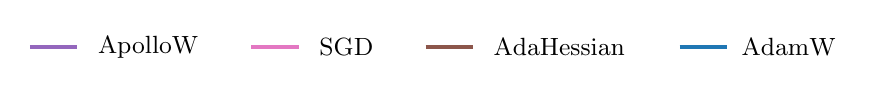
\begin{tikzpicture}[scale=0.75] % Nested TikZ environment
        \small 
        % AdaBelief
 \draw[mediumpurple148103189,  ultra thick] (0,0) -- ++(0.8,0);
 \node[anchor=west] at (1,0) {{ApolloW}}; % Increased spacing
 
 % Adam

 \draw[orchid227119194,  ultra thick] (3.75,0) -- ++(0.8,0);
 \node[anchor=west] at (4.75,0) {{SGD}}; % Increased spacing
 
 % AdaHessian
 \draw[sienna1408675,  ultra thick] (6.7,0) -- ++(0.8,0);
 \node[anchor=west] at (7.7,0) {{AdaHessian}}; % Increased spacing
 
 % Apollo
 \draw[steelblue31119180,  ultra thick] (11,0) -- ++(0.8,0);
 \node[anchor=west] at (11.9,0) {{AdamW}}; % Increased spacing
    
\end{tikzpicture}
};
    \end{tikzpicture}
     \\ % Replace with the correct path to your .tex file
    \end{tabular}
    \caption{Evaluation of optimizers on CIFAR-10 using ResNet-110 with the \emph{milestone} learning rate scheduler, where hyperparameters
    are held constant across all optimizers. For better visualization we applied a polynomial transformation, with $\hat{x}=x^\alpha$ and $\alpha=5$, for every $x \in \mathcal{D}$ in the output data $ \mathcal{D}$.}
    \label{fig:cifar-10-milestone-real}
\end{figure}

\begin{figure}[h!]
    \centering
    \begin{tabular}{cc}
        % This file was created with tikzplotlib v0.10.1.
\begin{tikzpicture}[scale=0.75]

    \definecolor{crimson2143940}{RGB}{214,39,40}
    \definecolor{darkgrey176}{RGB}{176,176,176}
    \definecolor{darkorange25512714}{RGB}{255,127,14}
    \definecolor{forestgreen4416044}{RGB}{44,160,44}
    \definecolor{lightgrey204}{RGB}{204,204,204}
    \definecolor{mediumpurple148103189}{RGB}{148,103,189}
    \definecolor{orchid227119194}{RGB}{227,119,194}
    \definecolor{sienna1408675}{RGB}{140,86,75}
    \definecolor{steelblue31119180}{RGB}{31,119,180}
    
    \begin{groupplot}[group style={group size=2 by 2,
        horizontal sep=1cm,  % Adjust horizontal spacing
        vertical sep=2cm}]
    \nextgroupplot[
    tick align=outside,
    tick pos=left,
    title={Polynom. Training Accuracy (step-lr)},
    x grid style={darkgrey176},
    xlabel={Epochs},
    xmin=-8.15, xmax=171.15,
    xtick style={color=black},
    y grid style={darkgrey176},
    ymin=-0.0499197916810125, ymax=1.04947497706028,
    ytick style={color=black}
    ]
    \addplot [semithick, steelblue31119180]
    table {%
    0 0.0042832641079583
    1 0.0266082364421916
    2 0.05647560735111
    3 0.098814047029192
    4 0.143921510262216
    5 0.188488105949355
    6 0.224107349238684
    7 0.257313288782406
    8 0.2807593460326
    9 0.306125386199472
    10 0.334689537571092
    11 0.359931801840378
    12 0.375463588119478
    13 0.394473534221097
    14 0.420740092869011
    15 0.431109772404506
    16 0.444277070827815
    17 0.462242437030527
    18 0.479539211493279
    19 0.497421091656462
    20 0.503858169608739
    21 0.515612757929083
    22 0.531175630494315
    23 0.545578015706252
    24 0.551889479980605
    25 0.565081523459351
    26 0.573802731249303
    27 0.590016751607883
    28 0.600862659325479
    29 0.611615595525716
    30 0.619971798379827
    31 0.632461514531827
    32 0.644101065075882
    33 0.652721562445803
    34 0.659024487518356
    35 0.663581915613866
    36 0.672500657175816
    37 0.6907183492313
    38 0.685092585514229
    39 0.688869779840387
    40 0.710274396344925
    41 0.711694793174595
    42 0.721030741535746
    43 0.712453266761618
    44 0.725157926761258
    45 0.740289921042321
    46 0.741464300671298
    47 0.740779064910063
    48 0.75896022155197
    49 0.757265625080453
    50 0.766472637105615
    51 0.770705500466329
    52 0.783823503940085
    53 0.772828933383486
    54 0.784028280568258
    55 0.785873196876214
    56 0.794632285485429
    57 0.790603765928003
    58 0.804409569072624
    59 0.806397469592164
    60 0.812700866318208
    61 0.807969639179273
    62 0.81049021010767
    63 0.830345896101063
    64 0.835504776775547
    65 0.823294076405582
    66 0.833137116566929
    67 0.84318260549203
    68 0.843074076608184
    69 0.849387253191112
    70 0.841880996284519
    71 0.849933258195561
    72 0.856507247825973
    73 0.85047954395124
    74 0.862016590322445
    75 0.861795673719218
    76 0.861574802411312
    77 0.862016590322445
    78 0.860691769993589
    79 0.86478187249727
    80 0.92182819042019
    81 0.953492638799097
    82 0.965407237467091
    83 0.970497757984052
    84 0.971834531552624
    85 0.977440644991537
    86 0.97731849850135
    87 0.980498278694188
    88 0.983563559535474
    89 0.985652325867234
    90 0.982213892919874
    91 0.988977070834394
    92 0.984300366423927
    93 0.984423210490172
    94 0.984177534621546
    95 0.988730486181861
    96 0.990951519699253
    97 0.989963901469861
    98 0.988237464432872
    99 0.990581070537152
    100 0.991075027379098
    101 0.990457612105862
    102 0.991075027379098
    103 0.992063532215067
    104 0.992805428332213
    105 0.993176542797388
    106 0.991075027379098
    107 0.992434424813065
    108 0.992310781623722
    109 0.991075027379098
    110 0.99305282564679
    111 0.99218715075803
    112 0.990951519699253
    113 0.992929120825373
    114 0.992805428332213
    115 0.995033780184654
    116 0.993547768233472
    117 0.993795313520321
    118 0.994042908146009
    119 0.994909877985751
    120 0.996025442234843
    121 0.995157694727487
    122 0.996893794956395
    123 0.996273481242038
    124 0.996769707501676
    125 0.997886939551392
    126 0.997762753208669
    127 0.99801113825927
    128 0.997266131470862
    129 0.996893794956395
    130 0.99801113825927
    131 0.997886939551392
    132 0.997886939551392
    133 0.99801113825927
    134 0.99801113825927
    135 0.996769707501676
    136 0.997886939551392
    137 0.997142006940065
    138 0.997762753208669
    139 0.997638579230178
    140 0.99801113825927
    141 0.997638579230178
    142 0.998383808583067
    143 0.998756590226503
    144 0.998508056760799
    145 0.998880875516322
    146 0.998383808583067
    147 0.998508056760799
    148 0.998135349333226
    149 0.998632317308303
    150 0.998508056760799
    151 0.998508056760799
    152 0.998259572774184
    153 0.999005173178685
    154 0.999005173178685
    155 0.998632317308303
    156 0.997886939551392
    157 0.998756590226503
    158 0.999005173178685
    159 0.997762753208669
    160 0.998880875516322
    161 0.99801113825927
    162 0.999129483214514
    163 0.998632317308303
    };
    \addplot [semithick, darkorange25512714]
    table {%
    0 0.00459987722122012
    1 0.0288545146869175
    2 0.0673373516161438
    3 0.108382275812215
    4 0.146017908778203
    5 0.190923235456279
    6 0.226486226476294
    7 0.260139304272314
    8 0.288268290112989
    9 0.309859169805502
    10 0.330666625598927
    11 0.359492579461494
    12 0.374271929414639
    13 0.398807322780257
    14 0.405651270024247
    15 0.422922867626645
    16 0.441812330257934
    17 0.450224207888497
    18 0.460500453948094
    19 0.472259032177343
    20 0.494227318996516
    21 0.497492251435988
    22 0.511088458739165
    23 0.523347916105072
    24 0.540996560773425
    25 0.539628143204597
    26 0.552353577624982
    27 0.565239138521256
    28 0.566185567630793
    29 0.564293975466834
    30 0.578926223298446
    31 0.591731678033054
    32 0.59468082774275
    33 0.602353920741366
    34 0.609101283559065
    35 0.611447716849871
    36 0.622436790490986
    37 0.628076006341572
    38 0.628161762213419
    39 0.645326956522139
    40 0.647169292809602
    41 0.660273044974572
    42 0.654492133932954
    43 0.662507318259485
    44 0.660898032937532
    45 0.680234442559543
    46 0.675494786502887
    47 0.676950319211409
    48 0.68720945335373
    49 0.697592593364958
    50 0.684449357905418
    51 0.70348802482068
    52 0.698525727602866
    53 0.707723397505457
    54 0.710179783920142
    55 0.704897556369446
    56 0.704803517366889
    57 0.715683997284078
    58 0.715874404603958
    59 0.723620028101461
    60 0.72429253737481
    61 0.732595678896124
    62 0.729303989618661
    63 0.738921692698377
    64 0.738238337588877
    65 0.737165515391541
    66 0.743621200706724
    67 0.747062975042078
    68 0.752695418186592
    69 0.758860455505686
    70 0.75210093468253
    71 0.750814175646502
    72 0.751110963600595
    73 0.758561220314021
    74 0.762058177411586
    75 0.763661075677295
    76 0.763661075677295
    77 0.758660954887538
    78 0.77770007229593
    79 0.767176819709774
    80 0.855848024258407
    81 0.898979233534559
    82 0.917523525326198
    83 0.929312231311833
    84 0.939327040969814
    85 0.942763541836939
    86 0.943475796110886
    87 0.949547355315588
    88 0.956850426177496
    89 0.956970521870567
    90 0.959134307213301
    91 0.961181474409778
    92 0.966617324100584
    93 0.961302004777847
    94 0.969162455822654
    95 0.967465106495774
    96 0.973294509553404
    97 0.973416253544139
    98 0.973416253544139
    99 0.974634363629828
    100 0.975853692861762
    101 0.977684974610361
    102 0.978785062610857
    103 0.979641371041958
    104 0.975365814812895
    105 0.978296012424459
    106 0.979886140640976
    107 0.978785062610857
    108 0.980008543786281
    109 0.976707949206047
    110 0.981233248136972
    111 0.980253386773063
    112 0.980375826616374
    113 0.981600898098424
    114 0.981968658252935
    115 0.97915197858462
    116 0.980620743007421
    117 0.979763749726508
    118 0.986021299780942
    119 0.983931907804706
    120 0.987621463838396
    121 0.989840504578549
    122 0.992434424813065
    123 0.992929120825373
    124 0.991198547373383
    125 0.99255808032698
    126 0.993547768233472
    127 0.99305282564679
    128 0.995281621615173
    129 0.995281621615173
    130 0.994042908146009
    131 0.994909877985751
    132 0.996025442234843
    133 0.995281621615173
    134 0.994166723963222
    135 0.99429055211791
    136 0.995033780184654
    137 0.995901441258672
    138 0.995777452632888
    139 0.994662110616046
    140 0.99429055211791
    141 0.995157694727487
    142 0.994785988129856
    143 0.996149455562325
    144 0.995033780184654
    145 0.995405560848633
    146 0.996149455562325
    147 0.996149455562325
    148 0.995529512428791
    149 0.996521569661856
    150 0.996025442234843
    151 0.996149455562325
    152 0.997390268362198
    153 0.996769707501676
    154 0.997266131470862
    155 0.997142006940065
    156 0.996893794956395
    157 0.996645632403804
    158 0.996893794956395
    159 0.996769707501676
    160 0.997017894768884
    161 0.997762753208669
    162 0.996645632403804
    163 0.998135349333226
    };
    \addplot [semithick, forestgreen4416044]
    table {%
    0 0.00413625898867581
    1 0.0261061574754945
    2 0.0566881376205757
    3 0.0947804287431828
    4 0.133722925106089
    5 0.172708267671051
    6 0.204875350676456
    7 0.242626277232976
    8 0.272263442404073
    9 0.301663832590208
    10 0.321430145376741
    11 0.348222421306439
    12 0.370996392489956
    13 0.389007065565783
    14 0.411303800163352
    15 0.428009186595452
    16 0.445253017388151
    17 0.460901983122614
    18 0.481269248988496
    19 0.499916534027004
    20 0.503067860358207
    21 0.521276191391511
    22 0.536597128081822
    23 0.540692228341803
    24 0.557245479949332
    25 0.566027741471426
    26 0.580615320000402
    27 0.591077903179208
    28 0.606845479134456
    29 0.611447716849871
    30 0.616922679353826
    31 0.630050762566884
    32 0.648575799842542
    33 0.651484443981876
    34 0.657155193483348
    35 0.680051657543117
    36 0.674314010642179
    37 0.683714832329468
    38 0.69294186864818
    39 0.706120977109401
    40 0.69861909591984
    41 0.711600029414354
    42 0.732304758528539
    43 0.733857402428575
    44 0.737262993112153
    45 0.745881505590412
    46 0.754183271719225
    47 0.756966893115516
    48 0.758062704768888
    49 0.774957044076834
    50 0.769090781778836
    51 0.780144835217688
    52 0.781778089998967
    53 0.778107106580209
    54 0.801591403686015
    55 0.802529913097032
    56 0.798573288823581
    57 0.809544259918907
    58 0.81989230299087
    59 0.826279881903524
    60 0.826173097044676
    61 0.838417895279626
    62 0.837553903292801
    63 0.840797550278307
    64 0.830560339398414
    65 0.840364484333198
    66 0.846879243180435
    67 0.849605621509672
    68 0.850916774769416
    69 0.848732417625013
    70 0.861795673719218
    71 0.864117558489391
    72 0.855408767429102
    73 0.869554755329872
    74 0.876697583797786
    75 0.866555374164734
    76 0.866666314553036
    77 0.873678501574088
    78 0.886030768754388
    79 0.886708524990367
    80 0.923344469981361
    81 0.954331200507114
    82 0.966738399470453
    83 0.971591372314581
    84 0.973903351339401
    85 0.976952132296705
    86 0.983072600122528
    87 0.982704509240213
    88 0.981355785881978
    89 0.983809112788409
    90 0.98466893541793
    91 0.986636501850549
    92 0.988360701427909
    93 0.985652325867234
    94 0.986636501850549
    95 0.989840504578549
    96 0.989840504578549
    97 0.990334165984407
    98 0.990334165984407
    99 0.98848395071714
    100 0.992063532215067
    101 0.990828024332928
    102 0.989840504578549
    103 0.991816332093646
    104 0.99218715075803
    105 0.99132207968303
    106 0.990828024332928
    107 0.99255808032698
    108 0.992805428332213
    109 0.991692750513346
    110 0.994042908146009
    111 0.99305282564679
    112 0.991816332093646
    113 0.991692750513346
    114 0.99156918125209
    115 0.99218715075803
    116 0.992929120825373
    117 0.994662110616046
    118 0.995529512428791
    119 0.99255808032698
    120 0.995529512428791
    121 0.996025442234843
    122 0.995529512428791
    123 0.997390268362198
    124 0.996521569661856
    125 0.997390268362198
    126 0.995901441258672
    127 0.997638579230178
    128 0.997142006940065
    129 0.997017894768884
    130 0.997762753208669
    131 0.997886939551392
    132 0.998259572774184
    133 0.997266131470862
    134 0.997638579230178
    135 0.997142006940065
    136 0.998383808583067
    137 0.997886939551392
    138 0.997142006940065
    139 0.997886939551392
    140 0.998383808583067
    141 0.998135349333226
    142 0.997514417614995
    143 0.997886939551392
    144 0.998135349333226
    145 0.998259572774184
    146 0.998259572774184
    147 0.998756590226503
    148 0.998632317308303
    149 0.998632317308303
    150 0.99801113825927
    151 0.999005173178685
    152 0.998508056760799
    153 0.998383808583067
    154 0.998756590226503
    155 0.997886939551392
    156 0.999129483214514
    157 0.998756590226503
    158 0.99801113825927
    159 0.997638579230178
    160 0.998632317308303
    161 0.99801113825927
    162 0.998880875516322
    163 0.998880875516322
    };
    \addplot [semithick, crimson2143940]
    table {%
    0 0.00104857376199295
    1 0.0109037005064662
    2 0.0423348576039176
    3 0.101858388028028
    4 0.165387127234947
    5 0.215591665598852
    6 0.255637859604132
    7 0.295655351007798
    8 0.323240561539949
    9 0.351282353464822
    10 0.36858281365221
    11 0.401857574525769
    12 0.423798509928744
    13 0.438328633818228
    14 0.456301268166834
    15 0.46987471616341
    16 0.483073781079645
    17 0.496212620715768
    18 0.513419597529047
    19 0.521276191391511
    20 0.531175630494315
    21 0.540920464821598
    22 0.561466069932077
    23 0.567844868842498
    24 0.577160912073724
    25 0.581098642474244
    26 0.593532542254684
    27 0.594434617080487
    28 0.608683036703583
    29 0.614728008227373
    30 0.624056032046495
    31 0.623970724882005
    32 0.631944304652573
    33 0.640260386662928
    34 0.636524719286851
    35 0.651307866006499
    36 0.654758050720499
    37 0.653606368554733
    38 0.664747635834279
    39 0.675949371257549
    40 0.669517154451339
    41 0.682156059254482
    42 0.676677215888316
    43 0.694334473577926
    44 0.686933043795183
    45 0.683898404574974
    46 0.69173675264673
    47 0.697592593364958
    48 0.702643388815772
    49 0.703957617899656
    50 0.707723397505457
    51 0.712073949178442
    52 0.712168763424157
    53 0.71349722368039
    54 0.710842282672975
    55 0.716255340822339
    56 0.72640939378596
    57 0.717780707693032
    58 0.73036765042342
    59 0.72814504609746
    60 0.726698439088472
    61 0.729207354665886
    62 0.737848076007147
    63 0.72814504609746
    64 0.740876924703436
    65 0.734537511715261
    66 0.744308538694541
    67 0.74686595956939
    68 0.755077112574026
    69 0.750023199735682
    70 0.758660954887538
    71 0.748245941169079
    72 0.743523051031461
    73 0.760957747019842
    74 0.761657873707965
    75 0.756469216016943
    76 0.766975571889548
    77 0.753587848233793
    78 0.77465274157637
    79 0.762859289748063
    80 0.85969922410853
    81 0.919964735433434
    82 0.940155622158088
    83 0.950741514019809
    84 0.959254632171401
    85 0.964077542235277
    86 0.964923542282926
    87 0.974390644110259
    88 0.973903351339401
    89 0.980375826616374
    90 0.980253386773063
    91 0.984054715082111
    92 0.985652325867234
    93 0.985529359111827
    94 0.987867827203724
    95 0.988237464432872
    96 0.99156918125209
    97 0.988853772359191
    98 0.989963901469861
    99 0.990457612105862
    100 0.991939925993913
    101 0.99218715075803
    102 0.99156918125209
    103 0.99305282564679
    104 0.994042908146009
    105 0.994166723963222
    106 0.991939925993913
    107 0.993300272278086
    108 0.995033780184654
    109 0.9945382454434
    110 0.994909877985751
    111 0.995157694727487
    112 0.996149455562325
    113 0.994414392610996
    114 0.995529512428791
    115 0.996769707501676
    116 0.997266131470862
    117 0.996149455562325
    118 0.996769707501676
    119 0.995529512428791
    120 0.995901441258672
    121 0.996645632403804
    122 0.996521569661856
    123 0.997886939551392
    124 0.997266131470862
    125 0.997266131470862
    126 0.99801113825927
    127 0.99801113825927
    128 0.997266131470862
    129 0.997886939551392
    130 0.99801113825927
    131 0.997390268362198
    132 0.998259572774184
    133 0.998135349333226
    134 0.998383808583067
    135 0.998383808583067
    136 0.999005173178685
    137 0.999129483214514
    138 0.998508056760799
    139 0.998259572774184
    140 0.999005173178685
    141 0.99801113825927
    142 0.997886939551392
    143 0.998383808583067
    144 0.998135349333226
    145 0.997762753208669
    146 0.998880875516322
    147 0.997886939551392
    148 0.997762753208669
    149 0.998383808583067
    150 0.998880875516322
    151 0.999253805624734
    152 0.998632317308303
    153 0.998383808583067
    154 0.998383808583067
    155 0.998508056760799
    156 0.998756590226503
    157 0.999005173178685
    158 0.999502487572043
    159 0.998383808583067
    160 0.998383808583067
    161 0.999005173178685
    162 0.998632317308303
    163 0.998632317308303
    };
    \addplot [semithick, mediumpurple148103189]
    table {%
    0 0.00140679072261522
    1 0.0141910610356492
    2 0.0553979075654559
    3 0.118181137015722
    4 0.172403215698944
    5 0.22580449585469
    6 0.26154031892367
    7 0.298056590561512
    8 0.324047804845097
    9 0.347848115123627
    10 0.37495250614606
    11 0.390236099366061
    12 0.416463306597858
    13 0.42267295014648
    14 0.442459882955339
    15 0.446752799193044
    16 0.469331084235817
    17 0.487118784803986
    18 0.49813305600277
    19 0.505081510013887
    20 0.518695767250905
    21 0.52394104565951
    22 0.534182135506143
    23 0.548111013756756
    24 0.55506704055402
    25 0.554523496686069
    26 0.567528511921838
    27 0.578524637420945
    28 0.584652850817727
    29 0.591568180112403
    30 0.602436855330355
    31 0.605428590157549
    32 0.605428590157549
    33 0.607095793504403
    34 0.622692236502794
    35 0.626705185657932
    36 0.620820911844926
    37 0.632202867278875
    38 0.637218403527089
    39 0.630566732371795
    40 0.643401392583973
    41 0.643838616597144
    42 0.654669402189527
    43 0.647344972620936
    44 0.6532523310425
    45 0.653783444863887
    46 0.648927808409469
    47 0.663850782705611
    48 0.669697670817527
    49 0.667624081711577
    50 0.673678892539469
    51 0.668074424419349
    52 0.687025170430397
    53 0.686380491504141
    54 0.684908756872615
    55 0.686288434034919
    56 0.689423934569847
    57 0.684633087901381
    58 0.689978445869537
    59 0.686104348728709
    60 0.695078111159479
    61 0.687117306949647
    62 0.692200060212388
    63 0.697499334816742
    64 0.709517779213813
    65 0.69517111063903
    66 0.711315798698453
    67 0.694985121633316
    68 0.718639867904395
    69 0.701331123308454
    70 0.715017890698033
    71 0.701518469673969
    72 0.708856268277618
    73 0.71397215392055
    74 0.720552058478078
    75 0.706591975609924
    76 0.728531196777448
    77 0.708100860041207
    78 0.73152942269707
    79 0.723523996141183
    80 0.837553903292801
    81 0.896696692543551
    82 0.91798811771392
    83 0.926500041526486
    84 0.93472134773786
    85 0.945853086703538
    86 0.954451043183337
    87 0.95661027096294
    88 0.959254632171401
    89 0.967343958319601
    90 0.971591372314581
    91 0.971712945848841
    92 0.974268802635382
    93 0.977440644991537
    94 0.979029661035917
    95 0.978051560648462
    96 0.9845460668212
    97 0.983440801296999
    98 0.981723472571698
    99 0.985652325867234
    100 0.985652325867234
    101 0.985898296200873
    102 0.988237464432872
    103 0.987375149627771
    104 0.98577530489661
    105 0.987867827203724
    106 0.987991027321699
    107 0.988977070834394
    108 0.98848395071714
    109 0.98910038160839
    110 0.990704541279201
    111 0.99156918125209
    112 0.99132207968303
    113 0.992063532215067
    114 0.991445624308958
    115 0.991692750513346
    116 0.992805428332213
    117 0.991445624308958
    118 0.991816332093646
    119 0.992434424813065
    120 0.993300272278086
    121 0.993547768233472
    122 0.995653476356568
    123 0.995529512428791
    124 0.996769707501676
    125 0.996769707501676
    126 0.997017894768884
    127 0.996893794956395
    128 0.996769707501676
    129 0.996273481242038
    130 0.996149455562325
    131 0.996645632403804
    132 0.997514417614995
    133 0.997638579230178
    134 0.997886939551392
    135 0.997390268362198
    136 0.996397519274908
    137 0.996893794956395
    138 0.996645632403804
    139 0.997762753208669
    140 0.998383808583067
    141 0.997886939551392
    142 0.996645632403804
    143 0.997266131470862
    144 0.997390268362198
    145 0.998135349333226
    146 0.998259572774184
    147 0.997762753208669
    148 0.997266131470862
    149 0.998259572774184
    150 0.997638579230178
    151 0.998756590226503
    152 0.998259572774184
    153 0.99801113825927
    154 0.998756590226503
    155 0.998259572774184
    156 0.99937814041027
    157 0.998756590226503
    158 0.998383808583067
    159 0.997886939551392
    160 0.998383808583067
    161 0.998135349333226
    162 0.998508056760799
    163 0.999005173178685
    };
    \addplot [semithick, sienna1408675]
    table {%
    0 5.26978072282426e-05
    1 0.00139835130102698
    2 0.00574539984509666
    3 0.013020266488205
    4 0.024274527123119
    5 0.0384972173008099
    6 0.0537582422689399
    7 0.072732825139161
    8 0.0912271745771269
    9 0.11358934387401
    10 0.134745991789077
    11 0.15571405204764
    12 0.180634207891172
    13 0.195835240262992
    14 0.218008342064028
    15 0.24162626920895
    16 0.253846518650103
    17 0.274113769664907
    18 0.289604484422393
    19 0.308837271932726
    20 0.320177691534009
    21 0.33718457183908
    22 0.348597049641294
    23 0.36285250573444
    24 0.369199041582462
    25 0.391526988411089
    26 0.398151860253095
    27 0.409169157691054
    28 0.418132669532232
    29 0.427883012082269
    30 0.441877051389057
    31 0.446361162726693
    32 0.459030573831415
    33 0.470418851730744
    34 0.471917824290192
    35 0.483212815121343
    36 0.49458137030226
    37 0.493519824668305
    38 0.510870349354279
    39 0.512398679980901
    40 0.531850910893322
    41 0.539704093682056
    42 0.541910380379954
    43 0.545884546032927
    44 0.551271168438682
    45 0.561936598485404
    46 0.568953229233872
    47 0.574840493291048
    48 0.588387187183725
    49 0.573882505847562
    50 0.588549981413197
    51 0.586111847917177
    52 0.586517641365797
    53 0.613717192022245
    54 0.609017615800461
    55 0.613044053594622
    56 0.613128163581817
    57 0.626619588905211
    58 0.638781404419595
    59 0.629277441210301
    60 0.633756020923464
    61 0.640434564519473
    62 0.645239330995217
    63 0.637391919048205
    64 0.65254471626774
    65 0.643663698478041
    66 0.662149428675827
    67 0.651572747330168
    68 0.657599878264387
    69 0.657510922055672
    70 0.665106648374961
    71 0.667894258183128
    72 0.680325849805314
    73 0.674858778759361
    74 0.674858778759361
    75 0.66322356167833
    76 0.67358820046177
    77 0.690810881764623
    78 0.690255835286981
    79 0.692385452733544
    80 0.804096048743428
    81 0.868331784328754
    82 0.891918447053177
    83 0.902640965334699
    84 0.916943049382316
    85 0.929077621676487
    86 0.936490625203109
    87 0.940037217631632
    88 0.949070027946104
    89 0.955770107418319
    90 0.95661027096294
    91 0.965044447899038
    92 0.963956733541131
    93 0.966617324100584
    94 0.974756241676348
    95 0.973416253544139
    96 0.974634363629828
    97 0.976952132296705
    98 0.980498278694188
    99 0.980008543786281
    100 0.983072600122528
    101 0.981478335868823
    102 0.983686330032305
    103 0.983195321591444
    104 0.983072600122528
    105 0.985529359111827
    106 0.986390384185179
    107 0.98577530489661
    108 0.989593747710708
    109 0.986144315637737
    110 0.986882668641202
    111 0.98848395071714
    112 0.990334165984407
    113 0.988360701427909
    114 0.988360701427909
    115 0.989840504578549
    116 0.993300272278086
    117 0.991939925993913
    118 0.99255808032698
    119 0.993300272278086
    120 0.99305282564679
    121 0.993547768233472
    122 0.996025442234843
    123 0.995157694727487
    124 0.996893794956395
    125 0.996397519274908
    126 0.99801113825927
    127 0.996273481242038
    128 0.996149455562325
    129 0.996893794956395
    130 0.997017894768884
    131 0.997762753208669
    132 0.996769707501676
    133 0.996521569661856
    134 0.996645632403804
    135 0.998135349333226
    136 0.997762753208669
    137 0.99801113825927
    138 0.997390268362198
    139 0.997762753208669
    140 0.997514417614995
    141 0.997142006940065
    142 0.998135349333226
    143 0.998508056760799
    144 0.997638579230178
    145 0.997390268362198
    146 0.997886939551392
    147 0.997514417614995
    148 0.998383808583067
    149 0.998508056760799
    150 0.998508056760799
    151 0.99801113825927
    152 0.997142006940065
    153 0.998383808583067
    154 0.998632317308303
    155 0.998135349333226
    156 0.998259572774184
    157 0.998508056760799
    158 0.998632317308303
    159 0.998383808583067
    160 0.999129483214514
    161 0.998508056760799
    162 0.99937814041027
    163 0.998383808583067
    };
    \addplot [semithick, orchid227119194]
    table {%
    0 8.36112451390153e-05
    1 0.00126156351963938
    2 0.00490482331170972
    3 0.0104428625863238
    4 0.0180162515461387
    5 0.0290226811271349
    6 0.043679925404287
    7 0.0647346030780771
    8 0.0886373094464463
    9 0.115656469635116
    10 0.14138045757742
    11 0.171521001774092
    12 0.200503616149239
    13 0.22104101759936
    14 0.244595897040766
    15 0.270466821963176
    16 0.29392298191824
    17 0.309664314340781
    18 0.334223367370164
    19 0.354797961478686
    20 0.370265376423073
    21 0.381812884687197
    22 0.403600336925158
    23 0.424675602012245
    24 0.432507704047898
    25 0.444472123100826
    26 0.465067542460837
    27 0.476025361730643
    28 0.497990597955828
    29 0.508186450751468
    30 0.512981862370329
    31 0.529228672544387
    32 0.538793252147512
    33 0.55568875536683
    34 0.570698434559417
    35 0.575959761804804
    36 0.59042470631171
    37 0.595502119225825
    38 0.616077834530714
    39 0.623885427046819
    40 0.621415844635743
    41 0.639390065737562
    42 0.644888924068005
    43 0.655290143593081
    44 0.682889244977016
    45 0.673225529818989
    46 0.686564636078791
    47 0.695915464893292
    48 0.705556110482865
    49 0.706215156710354
    50 0.703018682378482
    51 0.723716070258378
    52 0.743326782772113
    53 0.740387729138718
    54 0.742934370595159
    55 0.76065785037857
    56 0.761457784949098
    57 0.761057733584103
    58 0.774145783175395
    59 0.778310687622652
    60 0.76576897168517
    61 0.785257839301777
    62 0.787721584605315
    63 0.80346930135354
    64 0.804723187188479
    65 0.806188032024899
    66 0.810069678694476
    67 0.812279417489506
    68 0.809544259918907
    69 0.820635478313154
    70 0.815655908812599
    71 0.829167249575683
    72 0.844051238987384
    73 0.837985810205692
    74 0.841339133759176
    75 0.862348050171252
    76 0.846770333812886
    77 0.844268509177488
    78 0.855628373293478
    79 0.861685232403785
    80 0.904935600155009
    81 0.946686269598877
    82 0.95181728378977
    83 0.962387322300209
    84 0.96371515248537
    85 0.967828623853394
    86 0.969647850076219
    87 0.970619222033711
    88 0.975121948973827
    89 0.975609729439766
    90 0.975243875795343
    91 0.97939665035895
    92 0.978907355711635
    93 0.981110722632887
    94 0.982336528625274
    95 0.979519004586412
    96 0.981110722632887
    97 0.981355785881978
    98 0.982459176579853
    99 0.982949890908296
    100 0.985529359111827
    101 0.986759579104756
    102 0.986267343772176
    103 0.986513436877663
    104 0.988730486181861
    105 0.98848395071714
    106 0.988114239731109
    107 0.987744639376262
    108 0.9892237046821
    109 0.987621463838396
    110 0.990334165984407
    111 0.988977070834394
    112 0.988977070834394
    113 0.989840504578549
    114 0.990704541279201
    115 0.989717119992471
    116 0.990457612105862
    117 0.991445624308958
    118 0.99132207968303
    119 0.988114239731109
    120 0.989963901469861
    121 0.993795313520321
    122 0.992434424813065
    123 0.992681748166389
    124 0.993300272278086
    125 0.992929120825373
    126 0.992063532215067
    127 0.993919104665349
    128 0.992310781623722
    129 0.993424014089807
    130 0.994414392610996
    131 0.99255808032698
    132 0.99305282564679
    133 0.992805428332213
    134 0.996025442234843
    135 0.994042908146009
    136 0.991816332093646
    137 0.995281621615173
    138 0.99305282564679
    139 0.992063532215067
    140 0.995033780184654
    141 0.993300272278086
    142 0.995281621615173
    143 0.994662110616046
    144 0.995777452632888
    145 0.992310781623722
    146 0.993300272278086
    147 0.995157694727487
    148 0.9945382454434
    149 0.993795313520321
    150 0.99429055211791
    151 0.992805428332213
    152 0.993919104665349
    153 0.994662110616046
    154 0.994042908146009
    155 0.993176542797388
    156 0.995529512428791
    157 0.994042908146009
    158 0.993919104665349
    159 0.993424014089807
    160 0.993795313520321
    161 0.997390268362198
    162 0.993919104665349
    163 0.994662110616046
    };
    
    \nextgroupplot[
    tick align=outside,
    tick pos=left,
    title={Polynom. Test Accuracy (step-lr)},
    x grid style={darkgrey176},
    xlabel={Epochs},
    xmin=-8.15, xmax=171.15,
    xtick style={color=black},
    y grid style={darkgrey176},
    ymin=-0.0330693420981112, ymax=0.699475361679688,
    ytick style={color=black}
    ]
    \addplot [semithick, steelblue31119180]
    table {%
    0 0.0159035730352526
    1 0.0245055240745182
    2 0.064527065727614
    3 0.109887761820673
    4 0.109221777348323
    5 0.16058659519572
    6 0.159571797607686
    7 0.222839327143729
    8 0.246561038215834
    9 0.268317981879493
    10 0.18199177743074
    11 0.140328890928603
    12 0.262405149458153
    13 0.242918903246215
    14 0.225793147602503
    15 0.24528928831467
    16 0.311412986067274
    17 0.28922385695651
    18 0.369241087117621
    19 0.3530298958533
    20 0.275205519208526
    21 0.362036391588058
    22 0.341714437029492
    23 0.385358836250296
    24 0.336779421593888
    25 0.391315518587741
    26 0.377231100648871
    27 0.38970460062212
    28 0.402505898303966
    29 0.403449861065241
    30 0.378127348998841
    31 0.397112340986687
    32 0.3444116232029
    33 0.41564141243876
    34 0.404632304160866
    35 0.423194787057026
    36 0.429862640753325
    37 0.463945942229283
    38 0.420013989604323
    39 0.454254549791637
    40 0.395249934418099
    41 0.480827615907949
    42 0.437117753586536
    43 0.443195774987756
    44 0.468187705464067
    45 0.468453842170164
    46 0.403686128253106
    47 0.441416078788356
    48 0.494294573137247
    49 0.464210148339872
    50 0.438378475388319
    51 0.454254549791637
    52 0.467124367939556
    53 0.387183880751436
    54 0.456596868042102
    55 0.432852978021744
    56 0.446260034627646
    57 0.494850584974289
    58 0.43510663322009
    59 0.477034336874151
    60 0.440401679404048
    61 0.489588621905631
    62 0.471924646514628
    63 0.504379598076537
    64 0.476494399932492
    65 0.468453842170164
    66 0.492906729861853
    67 0.512622777924262
    68 0.502124383278527
    69 0.505227389679244
    70 0.513195220946946
    71 0.487111787418606
    72 0.498756693337167
    73 0.450372055059128
    74 0.496242803835597
    75 0.512908935546875
    76 0.491245434677605
    77 0.497917600840012
    78 0.486014194833338
    79 0.495685540776928
    80 0.588570333225214
    81 0.593057343951948
    82 0.598866524758463
    83 0.599190586723145
    84 0.596925096120781
    85 0.601137905804245
    86 0.60211346208346
    87 0.601137905804245
    88 0.601462950625131
    89 0.603742203454631
    90 0.603416173543536
    91 0.603742203454631
    92 0.604394686051705
    93 0.595311088045607
    94 0.599514788959209
    95 0.608649586883199
    96 0.602438928812115
    97 0.599190586723145
    98 0.600163614427623
    99 0.606682819075251
    100 0.607337842571827
    101 0.610292453522713
    102 0.606028360863207
    103 0.599190586723145
    104 0.605047732653145
    105 0.609306308430702
    106 0.602438928812115
    107 0.60211346208346
    108 0.598866524758463
    109 0.600488237751068
    110 0.604394686051705
    111 0.596279073350048
    112 0.594988705789528
    113 0.600163614427623
    114 0.60211346208346
    115 0.594344360273028
    116 0.603742203454631
    117 0.607993431719051
    118 0.611279875040054
    119 0.61095059263279
    120 0.604721138829035
    121 0.607010260140094
    122 0.613258552306386
    123 0.611609299409984
    124 0.612598424754793
    125 0.613919248810795
    126 0.615904755718705
    127 0.611938865788477
    128 0.61095059263279
    129 0.610292453522713
    130 0.61095059263279
    131 0.61095059263279
    132 0.610621452142302
    133 0.609306308430702
    134 0.61226857422144
    135 0.61226857422144
    136 0.611609299409984
    137 0.611609299409984
    138 0.610292453522713
    139 0.610621452142302
    140 0.608649586883199
    141 0.611279875040054
    142 0.609634881712767
    143 0.608977876836123
    144 0.611938865788477
    145 0.609306308430702
    146 0.611938865788477
    147 0.609963596728154
    148 0.609634881712767
    149 0.609306308430702
    150 0.608977876836123
    151 0.611279875040054
    152 0.609963596728154
    153 0.609634881712767
    154 0.61095059263279
    155 0.611938865788477
    156 0.61095059263279
    157 0.611938865788477
    158 0.610292453522713
    159 0.611609299409984
    160 0.609634881712767
    161 0.609963596728154
    162 0.607665566416219
    163 0.604721138829035
    };
    \addplot [semithick, darkorange25512714]
    table {%
    0 0.0138976810458799
    1 0.0597169931688682
    2 0.0774441083152062
    3 0.116815638077136
    4 0.110976912272078
    5 0.0983851503415281
    6 0.116640475958304
    7 0.201656860044255
    8 0.222105724517908
    9 0.215018138564276
    10 0.152936813309321
    11 0.194833915703985
    12 0.210628427194659
    13 0.306262940054886
    14 0.239631186242142
    15 0.220790109213771
    16 0.326282390534559
    17 0.206310705029083
    18 0.192078733005406
    19 0.339651199271979
    20 0.307781721800503
    21 0.308352815882217
    22 0.306452459195156
    23 0.351334880881658
    24 0.330087041557228
    25 0.322315478576512
    26 0.356011910122021
    27 0.393394521973586
    28 0.243864847985826
    29 0.312952155121889
    30 0.252999157086615
    31 0.395947516197151
    32 0.347125813881647
    33 0.342128285154667
    34 0.341921311001531
    35 0.343787689266857
    36 0.411065499912356
    37 0.377679012140355
    38 0.332913112739976
    39 0.423685846167607
    40 0.3940894832688
    41 0.416125448036024
    42 0.31469098859465
    43 0.367045843123009
    44 0.431355736364926
    45 0.455294390376698
    46 0.467655794924312
    47 0.475146696304944
    48 0.385358836250296
    49 0.444215318552448
    50 0.453735342451039
    51 0.442178104292394
    52 0.424423289443726
    53 0.450114169097583
    54 0.43185435581965
    55 0.415883373901779
    56 0.46341789090431
    57 0.46341789090431
    58 0.440655104232993
    59 0.472460437384154
    60 0.406767687440448
    61 0.401563703262636
    62 0.485466140993279
    63 0.425901256518903
    64 0.436865957652216
    65 0.479741368490421
    66 0.473533479043567
    67 0.392700541453861
    68 0.421479664541448
    69 0.462890320500361
    70 0.476224614864148
    71 0.502969141471122
    72 0.432103838398675
    73 0.467124367939556
    74 0.487386495164505
    75 0.484644987356976
    76 0.491245434677605
    77 0.443960256938511
    78 0.488486565803829
    79 0.453216609977071
    80 0.604721138829035
    81 0.608649586883199
    82 0.614911361158325
    83 0.61458051463572
    84 0.625573924451282
    85 0.619558192570682
    86 0.61226857422144
    87 0.617895396448631
    88 0.615242350149018
    89 0.606028360863207
    90 0.617231278500099
    91 0.612598424754793
    92 0.6185600859272
    93 0.613258552306386
    94 0.621558271157355
    95 0.617231278500099
    96 0.610292453522713
    97 0.617231278500099
    98 0.609306308430702
    99 0.610292453522713
    100 0.615573481653805
    101 0.611609299409984
    102 0.611609299409984
    103 0.609963596728154
    104 0.610621452142302
    105 0.61226857422144
    106 0.621892119184435
    107 0.612598424754793
    108 0.620557587232
    109 0.615573481653805
    110 0.606682819075251
    111 0.621892119184435
    112 0.612598424754793
    113 0.608977876836123
    114 0.61226857422144
    115 0.604394686051705
    116 0.61095059263279
    117 0.615573481653805
    118 0.607337842571827
    119 0.602764536267924
    120 0.623228946118094
    121 0.624903211610185
    122 0.625573924451282
    123 0.624233074179528
    124 0.624233074179528
    125 0.622894524068427
    126 0.623563511788995
    127 0.623228946118094
    128 0.6245680709917
    129 0.626581073417964
    130 0.627253226406341
    131 0.623898221127384
    132 0.626245213073296
    133 0.62256024559375
    134 0.62256024559375
    135 0.622894524068427
    136 0.622894524068427
    137 0.628262537331976
    138 0.62792595610252
    139 0.62994760914898
    140 0.626581073417964
    141 0.626581073417964
    142 0.627253226406341
    143 0.627253226406341
    144 0.628262537331976
    145 0.625573924451282
    146 0.629273147102568
    147 0.631298268192126
    148 0.628262537331976
    149 0.630622649388276
    150 0.631298268192126
    151 0.624903211610185
    152 0.627253226406341
    153 0.626581073417964
    154 0.62758951914277
    155 0.628599262877532
    156 0.631636294671948
    157 0.630285056971292
    158 0.628936132785591
    159 0.632312782019855
    160 0.630285056971292
    161 0.629610305874887
    162 0.631298268192126
    163 0.629273147102568
    };
    \addplot [semithick, forestgreen4416044]
    table {%
    0 0.00923219222754817
    1 0.0212068174880707
    2 0.0550539722795006
    3 0.067411745529337
    4 0.0702235326315588
    5 0.0746470185204544
    6 0.165854287187662
    7 0.0750767288398369
    8 0.230886471637795
    9 0.195362278554782
    10 0.269684334147671
    11 0.284548613358774
    12 0.178151381262253
    13 0.276250734560735
    14 0.258742190916091
    15 0.266448295894662
    16 0.316048750950811
    17 0.305694945144455
    18 0.376783614221638
    19 0.35218157257425
    20 0.337802817647072
    21 0.368361732701375
    22 0.37611318091434
    23 0.323105757658902
    24 0.307971992394218
    25 0.386042419633683
    26 0.377231100648871
    27 0.39455333618737
    28 0.43185435581965
    29 0.402977658564274
    30 0.389934406371491
    31 0.367484054442605
    32 0.463154045607747
    33 0.393394521973586
    34 0.445236737570332
    35 0.340681568613052
    36 0.462363230688863
    37 0.392469432384552
    38 0.436111265978953
    39 0.441923978951817
    40 0.420746316503446
    41 0.477574763166122
    42 0.446516152638936
    43 0.428869542781753
    44 0.403686128253106
    45 0.412746648929056
    46 0.456075519765793
    47 0.426147984154801
    48 0.462363230688863
    49 0.457902324840689
    50 0.443960256938511
    51 0.486014194833338
    52 0.45816377414576
    53 0.420013989604323
    54 0.472728515246852
    55 0.465268176728802
    56 0.456857720907804
    57 0.480827615907949
    58 0.488211362111775
    59 0.492906729861853
    60 0.494572516547412
    61 0.502687429177605
    62 0.475415992770654
    63 0.483551844715986
    64 0.478115679140956
    65 0.448826510687058
    66 0.488211362111775
    67 0.485466140993279
    68 0.497917600840012
    69 0.518370256917478
    70 0.514054844239829
    71 0.456596868042102
    72 0.488486565803829
    73 0.520973383200144
    74 0.475954952008743
    75 0.47326503603514
    76 0.501280760513418
    77 0.505227389679244
    78 0.527380626373476
    79 0.510053102251162
    80 0.578101205930159
    81 0.568402791352012
    82 0.582207470519157
    83 0.585700197281782
    84 0.587293331464896
    85 0.584428180828231
    86 0.592414672421599
    87 0.589849555374837
    88 0.593057343951948
    89 0.584745977547647
    90 0.593378888806648
    91 0.585381985729327
    92 0.597895180037523
    93 0.587931554977186
    94 0.590810430858527
    95 0.593057343951948
    96 0.59821882146116
    97 0.598542603019638
    98 0.596925096120781
    99 0.593057343951948
    100 0.590169708187189
    101 0.581257806513348
    102 0.585700197281782
    103 0.58825087473664
    104 0.58189077803834
    105 0.595311088045607
    106 0.591451709893807
    107 0.595633610027442
    108 0.579362196193275
    109 0.587293331464896
    110 0.5946664632138
    111 0.595956271780447
    112 0.589529541517697
    113 0.584428180828231
    114 0.592093545655287
    115 0.595633610027442
    116 0.597248317412813
    117 0.595311088045607
    118 0.596602014781678
    119 0.596279073350048
    120 0.602764536267924
    121 0.59821882146116
    122 0.600488237751068
    123 0.602438928812115
    124 0.606355519331539
    125 0.602764536267924
    126 0.603742203454631
    127 0.605701343624516
    128 0.605047732653145
    129 0.603416173543536
    130 0.603416173543536
    131 0.603416173543536
    132 0.603090284496517
    133 0.603090284496517
    134 0.603090284496517
    135 0.598866524758463
    136 0.606682819075251
    137 0.601788136036336
    138 0.603416173543536
    139 0.603742203454631
    140 0.607010260140094
    141 0.606028360863207
    142 0.606355519331539
    143 0.603090284496517
    144 0.604068374275463
    145 0.605701343624516
    146 0.603090284496517
    147 0.602438928812115
    148 0.604068374275463
    149 0.602764536267924
    150 0.60211346208346
    151 0.601788136036336
    152 0.601137905804245
    153 0.602764536267924
    154 0.599839131512188
    155 0.600163614427623
    156 0.600488237751068
    157 0.599514788959209
    158 0.600163614427623
    159 0.601137905804245
    160 0.600163614427623
    161 0.602438928812115
    162 0.599514788959209
    163 0.603090284496517
    };
    \addplot [semithick, crimson2143940]
    table {%
    0 0.00416165033564885
    1 0.0169804706220101
    2 0.0539586428151158
    3 0.0580954474251689
    4 0.160699668416977
    5 0.184757177143038
    6 0.225941656639461
    7 0.162860190524721
    8 0.184883671166191
    9 0.249763502588184
    10 0.257420394495477
    11 0.299316362665976
    12 0.358798934227249
    13 0.306073514689548
    14 0.373663085628984
    15 0.336983902110989
    16 0.355371216988612
    17 0.272433737518282
    18 0.366389310063579
    19 0.329483959425691
    20 0.3940894832688
    21 0.386042419633683
    22 0.345870992395898
    23 0.418552394956363
    24 0.433102921991301
    25 0.391085061869409
    26 0.395947516197151
    27 0.398981761434421
    28 0.419282682777305
    29 0.312181811729307
    30 0.418552394956363
    31 0.347335304408967
    32 0.407243439069632
    33 0.359229251920898
    34 0.435859933997401
    35 0.35558467878987
    36 0.357510454827929
    37 0.412265760423778
    38 0.420257985176687
    39 0.414433293815621
    40 0.357724943935522
    41 0.404632304160866
    42 0.342749809064519
    43 0.415883373901779
    44 0.45816377414576
    45 0.451404781190356
    46 0.426147984154801
    47 0.43938914579569
    48 0.437873838080977
    49 0.362469812335218
    50 0.40510605695306
    51 0.455294390376698
    52 0.394785426378705
    53 0.400858215553534
    54 0.404395594032705
    55 0.423194787057026
    56 0.47326503603514
    57 0.469252978528409
    58 0.441162303884876
    59 0.467921689729198
    60 0.397112340986687
    61 0.388328040357416
    62 0.447028741441129
    63 0.438378475388319
    64 0.467390021008174
    65 0.467655794924312
    66 0.439136303619287
    67 0.355798243155354
    68 0.468453842170164
    69 0.500718975564277
    70 0.48766132683405
    71 0.49235246619383
    72 0.442178104292394
    73 0.438378475388319
    74 0.469786341713288
    75 0.472996714783376
    76 0.446516152638936
    77 0.427878281116946
    78 0.46341789090431
    79 0.408434765891167
    80 0.618227669723614
    81 0.6245680709917
    82 0.635364151704372
    83 0.636383888523671
    84 0.639450957378428
    85 0.634345722519177
    86 0.640134131415841
    87 0.637745573889419
    88 0.637064440154868
    89 0.641159987185074
    90 0.643558765856326
    91 0.641844621385535
    92 0.638768366751767
    93 0.641844621385535
    94 0.644932716606633
    95 0.642529840306101
    96 0.644589009133839
    97 0.646653453932698
    98 0.642872669153437
    99 0.646998041718719
    100 0.645620571403931
    101 0.644589009133839
    102 0.644932716606633
    103 0.644245448215771
    104 0.646653453932698
    105 0.6487231848347
    106 0.645276570681032
    107 0.642187157732405
    108 0.648032686563272
    109 0.648032686563272
    110 0.641159987185074
    111 0.644932716606633
    112 0.637064440154868
    113 0.646998041718719
    114 0.648032686563272
    115 0.644589009133839
    116 0.65079821198483
    117 0.642187157732405
    118 0.65079821198483
    119 0.652531454349777
    120 0.656706306072903
    121 0.656009017639253
    122 0.654964195674282
    123 0.655660595606732
    124 0.65775335035324
    125 0.655312321634139
    126 0.652878545541045
    127 0.655660595606732
    128 0.656009017639253
    129 0.655660595606732
    130 0.654616217679977
    131 0.656357587778906
    132 0.653920705399345
    133 0.656706306072903
    134 0.656706306072903
    135 0.655660595606732
    136 0.654964195674282
    137 0.655660595606732
    138 0.654616217679977
    139 0.654964195674282
    140 0.653920705399345
    141 0.654616217679977
    142 0.656357587778906
    143 0.652184510794062
    144 0.655312321634139
    145 0.653573171018701
    146 0.653225784414978
    147 0.652531454349777
    148 0.652531454349777
    149 0.653225784414978
    150 0.652184510794062
    151 0.65045200590054
    152 0.653573171018701
    153 0.652184510794062
    154 0.654616217679977
    155 0.653225784414978
    156 0.655660595606732
    157 0.653225784414978
    158 0.656357587778906
    159 0.654616217679977
    160 0.655312321634139
    161 0.653573171018701
    162 0.654964195674282
    163 0.654964195674282
    };
    \addplot [semithick, mediumpurple148103189]
    table {%
    0 0.00386628602266784
    1 0.0191230895558899
    2 0.019413267703762
    3 0.081368941096116
    4 0.0837588583875167
    5 0.216880624635336
    6 0.231946415619151
    7 0.0940338496591599
    8 0.232705898975394
    9 0.233772516681854
    10 0.204110077646742
    11 0.201250293926507
    12 0.291766628288406
    13 0.324889553970956
    14 0.31064567589201
    15 0.320936211528157
    16 0.366170674606112
    17 0.237768535457463
    18 0.329684888776603
    19 0.335147148300964
    20 0.401799086435102
    21 0.401328430417409
    22 0.363120721683193
    23 0.389245314166854
    24 0.357081785267157
    25 0.389015833384316
    26 0.348384274725938
    27 0.331094140642284
    28 0.406767687440448
    29 0.354731446600775
    30 0.382634179477148
    31 0.405580253385898
    32 0.419770107373297
    33 0.386726972753334
    34 0.395714879590066
    35 0.413468822989359
    36 0.389934406371491
    37 0.469519599532052
    38 0.385586589693254
    39 0.448826510687058
    40 0.399684606406478
    41 0.412746648929056
    42 0.368361732701375
    43 0.391315518587741
    44 0.465268176728802
    45 0.415399563607632
    46 0.415157827369066
    47 0.444470497382198
    48 0.33903417533559
    49 0.391776757950212
    50 0.460784841525592
    51 0.408673365467486
    52 0.438883577852724
    53 0.396180262203062
    54 0.482188191200383
    55 0.446260034627646
    56 0.388557196517892
    57 0.400388441533278
    58 0.417094872072304
    59 0.429862640753325
    60 0.343787689266857
    61 0.459472812646799
    62 0.469519599532052
    63 0.360091125929277
    64 0.43435437435238
    65 0.362469812335218
    66 0.398981761434421
    67 0.45816377414576
    68 0.422459052208903
    69 0.400623273457335
    70 0.374552547462951
    71 0.464738921662782
    72 0.41564141243876
    73 0.451921854195893
    74 0.436865957652216
    75 0.44856933300032
    76 0.383540680324987
    77 0.449083806318157
    78 0.504379598076537
    79 0.4865627435301
    80 0.625238496081278
    81 0.640817889237908
    82 0.642529840306101
    83 0.646998041718719
    84 0.652531454349777
    85 0.653225784414978
    86 0.652878545541045
    87 0.654268387604053
    88 0.647687657987049
    89 0.656357587778906
    90 0.644589009133839
    91 0.654964195674282
    92 0.656706306072903
    93 0.647687657987049
    94 0.648377862163495
    95 0.653225784414978
    96 0.654268387604053
    97 0.645276570681032
    98 0.648032686563272
    99 0.655312321634139
    100 0.654616217679977
    101 0.654616217679977
    102 0.644245448215771
    103 0.648032686563272
    104 0.648032686563272
    105 0.652531454349777
    106 0.652531454349777
    107 0.65845212151121
    108 0.657404187312832
    109 0.65045200590054
    110 0.655660595606732
    111 0.656009017639253
    112 0.649068654623879
    113 0.65775335035324
    114 0.649414271578035
    115 0.661603944858175
    116 0.653920705399345
    117 0.643902033805554
    118 0.649760035744181
    119 0.649760035744181
    120 0.65845212151121
    121 0.660201647895845
    122 0.656706306072903
    123 0.656357587778906
    124 0.659501391650146
    125 0.660902498838952
    126 0.660551999006557
    127 0.663360165850962
    128 0.660902498838952
    129 0.661253147440374
    130 0.660902498838952
    131 0.65775335035324
    132 0.662305986332384
    133 0.663711857162031
    134 0.664063697621237
    135 0.663360165850962
    136 0.663711857162031
    137 0.660201647895845
    138 0.663008623640606
    139 0.663360165850962
    140 0.665120114362059
    141 0.663360165850962
    142 0.663008623640606
    143 0.664767826173802
    144 0.663008623640606
    145 0.662305986332384
    146 0.661954891139721
    147 0.662305986332384
    148 0.664415687276012
    149 0.664767826173802
    150 0.663711857162031
    151 0.661954891139721
    152 0.663008623640606
    153 0.661253147440374
    154 0.663360165850962
    155 0.664767826173802
    156 0.665120114362059
    157 0.666177875144333
    158 0.660201647895845
    159 0.660201647895845
    160 0.662657230483547
    161 0.664415687276012
    162 0.661954891139721
    163 0.663008623640606
    };
    \addplot [semithick, sienna1408675]
    table {%
    0 0.000228144437243303
    1 0.00221644471331296
    2 0.00402954527455905
    3 0.00790114319153757
    4 0.0212964867786413
    5 0.0366552352217643
    6 0.0562158160607255
    7 0.0782039792695489
    8 0.0767527597224619
    9 0.107652999549972
    10 0.0830894336061098
    11 0.0758179776096062
    12 0.0665692497218192
    13 0.105616336019952
    14 0.142472991692003
    15 0.128471942214844
    16 0.170902576618973
    17 0.139822215797499
    18 0.172333114755102
    19 0.151960900928675
    20 0.107817280000925
    21 0.0889182931827404
    22 0.170665080023368
    23 0.192470410552664
    24 0.25626825903046
    25 0.239009010318889
    26 0.28633957329329
    27 0.248638877812729
    28 0.262405149458153
    29 0.320739559443668
    30 0.338212872002316
    31 0.313337896668923
    32 0.32330356943065
    33 0.309879878961949
    34 0.18062155125766
    35 0.372332061980255
    36 0.362036391588058
    37 0.285622110428602
    38 0.383087215395442
    39 0.325684876855673
    40 0.297090696285416
    41 0.330288265058659
    42 0.399215933139106
    43 0.375889915349632
    44 0.345244943943517
    45 0.385814450808326
    46 0.214305214329708
    47 0.412987261402947
    48 0.414916203683747
    49 0.424423289443726
    50 0.346497948712925
    51 0.450114169097583
    52 0.38970460062212
    53 0.429365862069865
    54 0.376336552556047
    55 0.360738616398357
    56 0.451146422233535
    57 0.399684606406478
    58 0.417580261141208
    59 0.392931759382833
    60 0.419770107373297
    61 0.331901588473774
    62 0.295982839112625
    63 0.317606213749653
    64 0.369241087117621
    65 0.44856933300032
    66 0.417823125076211
    67 0.468986478661066
    68 0.442178104292394
    69 0.457118692979656
    70 0.407005507644097
    71 0.429117645021312
    72 0.407719635742398
    73 0.461836621141393
    74 0.395714879590066
    75 0.397812550653377
    76 0.414916203683747
    77 0.477304488830567
    78 0.420502094129892
    79 0.429117645021312
    80 0.618227669723614
    81 0.63502453007877
    82 0.63400653649201
    83 0.632651242980957
    84 0.638086359162116
    85 0.632989848862185
    86 0.634345722519177
    87 0.651144565469259
    88 0.642872669153437
    89 0.638768366751767
    90 0.645276570681032
    91 0.639450957378428
    92 0.634685053699235
    93 0.646998041718719
    94 0.641159987185074
    95 0.642529840306101
    96 0.637745573889419
    97 0.647342776387852
    98 0.643902033805554
    99 0.642187157732405
    100 0.641844621385535
    101 0.639450957378428
    102 0.641159987185074
    103 0.636043830880205
    104 0.636724091599678
    105 0.638768366751767
    106 0.639792471447425
    107 0.649760035744181
    108 0.650105947169338
    109 0.644245448215771
    110 0.634345722519177
    111 0.643902033805554
    112 0.643215644321234
    113 0.627253226406341
    114 0.640134131415841
    115 0.650105947169338
    116 0.644589009133839
    117 0.642529840306101
    118 0.641502231218689
    119 0.646998041718719
    120 0.653920705399345
    121 0.653225784414978
    122 0.652184510794062
    123 0.655660595606732
    124 0.652184510794062
    125 0.652184510794062
    126 0.653573171018701
    127 0.654964195674282
    128 0.654964195674282
    129 0.653573171018701
    130 0.653225784414978
    131 0.657404187312832
    132 0.654268387604053
    133 0.655660595606732
    134 0.657404187312832
    135 0.655660595606732
    136 0.655312321634139
    137 0.655312321634139
    138 0.652184510794062
    139 0.659501391650146
    140 0.655312321634139
    141 0.655312321634139
    142 0.659851445459482
    143 0.65775335035324
    144 0.658102661736945
    145 0.65845212151121
    146 0.661253147440374
    147 0.657404187312832
    148 0.655312321634139
    149 0.657404187312832
    150 0.65845212151121
    151 0.65775335035324
    152 0.655312321634139
    153 0.65845212151121
    154 0.65845212151121
    155 0.653225784414978
    156 0.654268387604053
    157 0.653920705399345
    158 0.654616217679977
    159 0.653573171018701
    160 0.653920705399345
    161 0.653225784414978
    162 0.656357587778906
    163 0.657055172568467
    };
    \addplot [semithick, orchid227119194]
    table {%
    0 0.000490905692556255
    1 0.00384340188443419
    2 0.010290097751664
    3 0.0179576500102808
    4 0.0259188397418383
    5 0.0413134509947015
    6 0.0499720052419414
    7 0.08696320064052
    8 0.099999751782046
    9 0.130949447086293
    10 0.13841130690703
    11 0.17827424427914
    12 0.20714081677142
    13 0.218755994681746
    14 0.249441766829572
    15 0.235763753185664
    16 0.25495658803589
    17 0.270198148937282
    18 0.281878986762001
    19 0.295430151281542
    20 0.296721042609333
    21 0.301929811356855
    22 0.31956167030393
    23 0.332305902700959
    24 0.314303914854819
    25 0.336370758346832
    26 0.355371216988612
    27 0.358369029011584
    28 0.370563266787126
    29 0.37255363544576
    30 0.320543003769073
    31 0.343579912354481
    32 0.355371216988612
    33 0.332103696364793
    34 0.339445424893392
    35 0.365952143534156
    36 0.363772565797882
    37 0.378576111527225
    38 0.385814450808326
    39 0.385586589693254
    40 0.38809899232772
    41 0.382634179477148
    42 0.375666755824134
    43 0.40795790106767
    44 0.415399563607632
    45 0.433352981408416
    46 0.413950833688895
    47 0.419526338444119
    48 0.404158994697954
    49 0.414674692512365
    50 0.423931546605309
    51 0.443195774987756
    52 0.419039140333383
    53 0.450372055059128
    54 0.420013989604323
    55 0.464738921662782
    56 0.438883577852724
    57 0.448312273217391
    58 0.415157827369066
    59 0.446772388229937
    60 0.437117753586536
    61 0.445492385667387
    62 0.395482352343236
    63 0.424669331923747
    64 0.461573496364077
    65 0.472192481153878
    66 0.445492385667387
    67 0.439895179538866
    68 0.470854523040325
    69 0.465003488957338
    70 0.477304488830567
    71 0.459997265066368
    72 0.456075519765793
    73 0.479741368490421
    74 0.464738921662782
    75 0.43410385274505
    76 0.474608469472703
    77 0.462363230688863
    78 0.44090864571318
    79 0.458948838687605
    80 0.518947828177047
    81 0.5198151502589
    82 0.527966214397443
    83 0.528845571654813
    84 0.528259203410425
    85 0.53090196235163
    86 0.53090196235163
    87 0.531196253897808
    88 0.532079911660473
    89 0.532964745020853
    90 0.538298498455392
    91 0.529726100217028
    92 0.532374725434074
    93 0.530313770561037
    94 0.53385075515155
    95 0.535626310418194
    96 0.527966214397443
    97 0.537109545858732
    98 0.535626310418194
    99 0.536812636222068
    100 0.533555287616646
    101 0.53621921085869
    102 0.534737943225944
    103 0.532374725434074
    104 0.537406586856808
    105 0.536515857903242
    106 0.533555287616646
    107 0.536812636222068
    108 0.53948955562512
    109 0.536515857903242
    110 0.540384231308414
    111 0.535626310418194
    112 0.537703759259879
    113 0.534737943225944
    114 0.530019870229887
    115 0.532964745020853
    116 0.535626310418194
    117 0.536812636222068
    118 0.535922695044855
    119 0.534146353569081
    120 0.53385075515155
    121 0.53621921085869
    122 0.536515857903242
    123 0.537406586856808
    124 0.53503393455226
    125 0.536812636222068
    126 0.540085874297523
    127 0.538596065335049
    128 0.538596065335049
    129 0.537703759259879
    130 0.539191593876276
    131 0.539787649084315
    132 0.53948955562512
    133 0.538001063111539
    134 0.53948955562512
    135 0.541280093564038
    136 0.540384231308414
    137 0.537703759259879
    138 0.53948955562512
    139 0.538596065335049
    140 0.542476424390136
    141 0.541578978202561
    142 0.541280093564038
    143 0.540384231308414
    144 0.538893763794133
    145 0.539787649084315
    146 0.539787649084315
    147 0.539787649084315
    148 0.53948955562512
    149 0.541877994857264
    150 0.537109545858732
    151 0.537109545858732
    152 0.538596065335049
    153 0.537703759259879
    154 0.538596065335049
    155 0.537109545858732
    156 0.53948955562512
    157 0.537703759259879
    158 0.53621921085869
    159 0.536515857903242
    160 0.538893763794133
    161 0.538001063111539
    162 0.537109545858732
    163 0.537109545858732
    };
    
    \nextgroupplot[
    tick align=outside,
    tick pos=left,
    title={Log Train Loss (step-lr)},
    x grid style={darkgrey176},
    xlabel={Epochs},
    xmin=-8.15, xmax=171.15,
    xtick style={color=black},
    y grid style={darkgrey176},
    ymin=-7.13431766562462, ymax=1.29734248591826,
    ytick style={color=black}
    ]
    \addplot [semithick, steelblue31119180]
    table {%
    0 0.579863894890465
    1 0.346483934880301
    2 0.196818162665963
    3 0.037618944636633
    4 -0.0913330120660096
    5 -0.202712055883516
    6 -0.292732874350437
    7 -0.373894108943251
    8 -0.443902279335496
    9 -0.503032247298885
    10 -0.560132845905853
    11 -0.628093735801886
    12 -0.676590509964326
    13 -0.718628645236602
    14 -0.775967525275914
    15 -0.802960604735088
    16 -0.845340401123574
    17 -0.881688637217819
    18 -0.927706076804667
    19 -0.991181589739836
    20 -1.00592892232813
    21 -1.03142802522698
    22 -1.07804650299678
    23 -1.11998465417454
    24 -1.12983876936853
    25 -1.17415343088387
    26 -1.20906641144938
    27 -1.24288357699477
    28 -1.27307390082338
    29 -1.3144713067352
    30 -1.34286841109668
    31 -1.3770685227692
    32 -1.41737779431339
    33 -1.45485618860256
    34 -1.46965822047816
    35 -1.5045436736305
    36 -1.52206484488961
    37 -1.58957167304516
    38 -1.58228608181687
    39 -1.60050873489484
    40 -1.65375657914207
    41 -1.68536451570789
    42 -1.71800525110688
    43 -1.71012158759969
    44 -1.73873862019479
    45 -1.80108637473935
    46 -1.80359936060706
    47 -1.79858045172648
    48 -1.88848125896605
    49 -1.89981972984054
    50 -1.90543666222962
    51 -1.95511849293986
    52 -2.0086969122653
    53 -1.94754690120696
    54 -1.99385913074031
    55 -2.02911342054712
    56 -2.07734351576198
    57 -2.03879414791389
    58 -2.11784305270972
    59 -2.13807740008082
    60 -2.16296561501739
    61 -2.15507019791478
    62 -2.1631092459831
    63 -2.25619298345211
    64 -2.30715480975454
    65 -2.25373744579225
    66 -2.28057333808338
    67 -2.33769186252892
    68 -2.35681756697337
    69 -2.3984685132703
    70 -2.35218035572646
    71 -2.41651958413488
    72 -2.41043797932298
    73 -2.38532429708755
    74 -2.48213072725748
    75 -2.47162526449705
    76 -2.46561754491621
    77 -2.49526016477025
    78 -2.47078050597453
    79 -2.51301580032161
    80 -3.04527528275692
    81 -3.5345653510169
    82 -3.73708405703134
    83 -3.86067328196015
    84 -3.98614710030829
    85 -4.09995976393625
    86 -4.13535933282337
    87 -4.27951022807341
    88 -4.34052616409704
    89 -4.48530609032419
    90 -4.40861322003294
    91 -4.63943729755722
    92 -4.5752716541217
    93 -4.54640740748858
    94 -4.59904207817092
    95 -4.76525625417871
    96 -4.94811565729403
    97 -4.86361277676982
    98 -4.82283046620111
    99 -4.98171626846089
    100 -5.03726641810761
    101 -4.9075863036062
    102 -5.0896391768435
    103 -5.12585870531031
    104 -5.09550700374753
    105 -5.30618644719264
    106 -5.03772337561595
    107 -5.17569329500456
    108 -5.23028609599486
    109 -5.11953192316567
    110 -5.21953266502968
    111 -5.23690332129936
    112 -5.10607883856541
    113 -5.24419773359271
    114 -5.23863205092325
    115 -5.53502696328566
    116 -5.3490172276353
    117 -5.31697700058241
    118 -5.45835487549965
    119 -5.57610129606647
    120 -5.68396279234122
    121 -5.68573880433091
    122 -6.00424247926553
    123 -5.81078126383314
    124 -5.93041140465947
    125 -6.13392873772031
    126 -6.1536931500692
    127 -6.15704545283863
    128 -6.04299745804355
    129 -5.94413290377684
    130 -6.21200199974535
    131 -6.15358754863076
    132 -6.12270147091513
    133 -6.29085071696804
    134 -6.26133452834878
    135 -6.03909239157431
    136 -6.27182399953617
    137 -6.26050964656348
    138 -6.18087720258816
    139 -6.16691252595399
    140 -6.24292522455336
    141 -6.25673558518992
    142 -6.41982796510928
    143 -6.37414752457636
    144 -6.32110767188235
    145 -6.43417815735749
    146 -6.43605970219351
    147 -6.37896150734267
    148 -6.34097841906308
    149 -6.56073841244846
    150 -6.47948928037379
    151 -6.49469826359907
    152 -6.5137099034608
    153 -6.52998917764155
    154 -6.48753864811158
    155 -6.51072171550326
    156 -6.37797530553407
    157 -6.55823922557703
    158 -6.69494044282096
    159 -6.32181857351429
    160 -6.67280514350997
    161 -6.40481471121168
    162 -6.70423653000026
    163 -6.49697302507852
    };
    \addplot [semithick, darkorange25512714]
    table {%
    0 0.570568131739019
    1 0.330065680743568
    2 0.14698848589907
    3 0.00903742527498221
    4 -0.103595936692885
    5 -0.217761755807463
    6 -0.301955172068859
    7 -0.379426498406708
    8 -0.445437019830584
    9 -0.505291484568103
    10 -0.555652798779513
    11 -0.611993596156412
    12 -0.65821701615397
    13 -0.710191294176687
    14 -0.730657608163752
    15 -0.777914871420426
    16 -0.82027366381488
    17 -0.852782568545207
    18 -0.878908551643391
    19 -0.908950579054182
    20 -0.956891294819604
    21 -0.974109386335208
    22 -1.00991113379332
    23 -1.04393936915638
    24 -1.06694207208622
    25 -1.08918139308932
    26 -1.11624309868245
    27 -1.14605599731381
    28 -1.15803436230186
    29 -1.15267286191498
    30 -1.20217491563639
    31 -1.24755493693822
    32 -1.25533403615604
    33 -1.26384527493268
    34 -1.28821904530756
    35 -1.3108327157133
    36 -1.3375872772361
    37 -1.35405795197754
    38 -1.38066162172672
    39 -1.40439488183533
    40 -1.4094821967659
    41 -1.45576158663084
    42 -1.44032525773103
    43 -1.47475029904257
    44 -1.48980228907687
    45 -1.51521863689789
    46 -1.52767572117261
    47 -1.54098258910326
    48 -1.54441820813702
    49 -1.58802559173961
    50 -1.57293492860125
    51 -1.62900375921365
    52 -1.62748242312222
    53 -1.64349265454994
    54 -1.6698192519558
    55 -1.64827500671122
    56 -1.63759901408345
    57 -1.67521321845465
    58 -1.67385222583881
    59 -1.71318978803092
    60 -1.72296108415212
    61 -1.73066563763642
    62 -1.74121988433968
    63 -1.78477846537389
    64 -1.77590950092467
    65 -1.77031273372285
    66 -1.78661491534442
    67 -1.80933950637739
    68 -1.83221520068996
    69 -1.85869392787357
    70 -1.81844572987033
    71 -1.81584107749733
    72 -1.84727727620709
    73 -1.85424318596318
    74 -1.86968625359557
    75 -1.89326718173336
    76 -1.88645913178845
    77 -1.87797556820967
    78 -1.95281035535704
    79 -1.9069095109175
    80 -2.37695573490097
    81 -2.74808831306905
    82 -2.90492514032347
    83 -3.05603482790094
    84 -3.19715855875816
    85 -3.27606539587877
    86 -3.33271442152935
    87 -3.42946551672066
    88 -3.52036717892738
    89 -3.55427061744438
    90 -3.68229737670255
    91 -3.67340029816238
    92 -3.8161130412308
    93 -3.71020730234846
    94 -3.89844667050192
    95 -3.84111178232613
    96 -4.05280188314008
    97 -4.00997759362986
    98 -4.02176188196521
    99 -4.11069343867749
    100 -4.11708403428432
    101 -4.18915680552443
    102 -4.21400262459146
    103 -4.30572184779024
    104 -4.24755662734153
    105 -4.2582338072147
    106 -4.27070358681882
    107 -4.29418373585697
    108 -4.303429340047
    109 -4.32334996646072
    110 -4.40093511426986
    111 -4.39315711366975
    112 -4.41878287587468
    113 -4.44604097223002
    114 -4.40431355774596
    115 -4.35964447688032
    116 -4.39555037395951
    117 -4.35210543082321
    118 -4.65371312405803
    119 -4.56572913996139
    120 -4.75270643398381
    121 -4.90599888303809
    122 -5.1440744225774
    123 -5.14072911015279
    124 -5.02860444839033
    125 -5.19965480088201
    126 -5.25184527075364
    127 -5.2049107483507
    128 -5.40586635276435
    129 -5.42355485756494
    130 -5.34431599797292
    131 -5.39918510568253
    132 -5.50657096090185
    133 -5.4588434263802
    134 -5.4888613365476
    135 -5.45186740020672
    136 -5.51218990139628
    137 -5.58197973401291
    138 -5.50957121345032
    139 -5.46577166661482
    140 -5.46365277181588
    141 -5.5318125423821
    142 -5.54804815592359
    143 -5.6382537251785
    144 -5.53141244147609
    145 -5.58251188185481
    146 -5.65552772796269
    147 -5.73284943328117
    148 -5.51468559956488
    149 -5.70204682202945
    150 -5.64395590490361
    151 -5.70279700358372
    152 -5.87432095438553
    153 -5.8140061155969
    154 -5.77441621233875
    155 -5.80973450917083
    156 -5.75964630936919
    157 -5.84504056859453
    158 -5.79596980583968
    159 -5.79552877902006
    160 -5.83694032897551
    161 -5.91918402450541
    162 -5.91333004678715
    163 -6.04332269804098
    };
    \addplot [semithick, forestgreen4416044]
    table {%
    0 0.574269706127844
    1 0.346135821799611
    2 0.192305296267402
    3 0.0472599746767135
    4 -0.0668201919934801
    5 -0.17140919434587
    6 -0.253004868968121
    7 -0.340515861252589
    8 -0.419460631361079
    9 -0.488825400913659
    10 -0.543036539382558
    11 -0.605327208634108
    12 -0.656369969034024
    13 -0.702488370591671
    14 -0.758538061491405
    15 -0.793737173890963
    16 -0.835592988904872
    17 -0.88937791487312
    18 -0.925563981873413
    19 -0.975999881431665
    20 -0.99811957696192
    21 -1.03291906205901
    22 -1.08448242784244
    23 -1.1140276992291
    24 -1.15621111188183
    25 -1.17659210652132
    26 -1.20912945750671
    27 -1.26422114546658
    28 -1.28270688684862
    29 -1.32778345086224
    30 -1.33416057252968
    31 -1.37579025825948
    32 -1.43004342544148
    33 -1.45969684648932
    34 -1.47879397742738
    35 -1.54380931799733
    36 -1.52441460735706
    37 -1.55660697976134
    38 -1.6029290640435
    39 -1.64850434058797
    40 -1.65277913045385
    41 -1.69167403553699
    42 -1.7618185730511
    43 -1.75999740787927
    44 -1.76943260591872
    45 -1.79350382653481
    46 -1.87521756629114
    47 -1.88174007390038
    48 -1.89790929583746
    49 -1.95210694368445
    50 -1.94021580207154
    51 -1.99592291077324
    52 -2.02027235031223
    53 -2.01184406562192
    54 -2.08062713501209
    55 -2.11770056683563
    56 -2.11294804140828
    57 -2.14228635056729
    58 -2.21349731387164
    59 -2.26160261392514
    60 -2.24107602078155
    61 -2.30630780258492
    62 -2.315485086745
    63 -2.31294953781283
    64 -2.28200876934394
    65 -2.33478149780513
    66 -2.39087597991312
    67 -2.38155828830567
    68 -2.41377262442344
    69 -2.41585827855859
    70 -2.4995403293396
    71 -2.50829701294723
    72 -2.45874673265173
    73 -2.52689868689167
    74 -2.61889620264722
    75 -2.53668957777189
    76 -2.51005489681736
    77 -2.5832993686504
    78 -2.68548363742452
    79 -2.68523434121333
    80 -3.11466655681842
    81 -3.59878064857886
    82 -3.8511949954401
    83 -3.95849254430828
    84 -4.09219745737474
    85 -4.18642276652496
    86 -4.37009055743226
    87 -4.43734729925204
    88 -4.40189223946833
    89 -4.54042767096338
    90 -4.49303861498262
    91 -4.64029363481137
    92 -4.77342160358671
    93 -4.65855102111936
    94 -4.72392533297661
    95 -4.88826003318243
    96 -4.91937167273055
    97 -4.90019646912972
    98 -4.90241328762349
    99 -4.97112586402947
    100 -5.08874036878703
    101 -5.05925850985682
    102 -5.09056581240253
    103 -5.15597643130249
    104 -5.16673816394824
    105 -5.13523958324448
    106 -5.16519242841518
    107 -5.2485381675105
    108 -5.31219927690224
    109 -5.23897468797955
    110 -5.38009221604157
    111 -5.30899998686172
    112 -5.25777966599281
    113 -5.24089666194531
    114 -5.28355969666683
    115 -5.30286391127583
    116 -5.40966296909105
    117 -5.5148271083756
    118 -5.63431778635616
    119 -5.35189258596627
    120 -5.73250647076381
    121 -5.86153946648549
    122 -5.80129812476636
    123 -6.04676692790231
    124 -5.92959513606747
    125 -6.01663937381435
    126 -5.85245245733991
    127 -6.09008768277351
    128 -6.06718832098548
    129 -5.99426848856679
    130 -6.17422475208379
    131 -6.19939403411145
    132 -6.29354042499807
    133 -6.08189782364921
    134 -6.20516624017298
    135 -6.16228306262049
    136 -6.31774530640406
    137 -6.32407520865149
    138 -6.16590258583918
    139 -6.20009232980487
    140 -6.379124379962
    141 -6.26517943616054
    142 -6.3034651545349
    143 -6.22342207787322
    144 -6.39164696488813
    145 -6.35221494728535
    146 -6.34670978915195
    147 -6.63317639260991
    148 -6.31494347640742
    149 -6.59379084861658
    150 -6.24881346798046
    151 -6.61626564434561
    152 -6.35078320316988
    153 -6.37473082573722
    154 -6.52724436869723
    155 -6.41219353295929
    156 -6.75106038600903
    157 -6.64079029883645
    158 -6.40189830142766
    159 -6.41506071270779
    160 -6.62937247804653
    161 -6.34314062401529
    162 -6.65281874215605
    163 -6.64408164104392
    };
    \addplot [semithick, crimson2143940]
    table {%
    0 0.68976154590591
    1 0.473829958448252
    2 0.254843411123742
    3 0.0291789789924686
    4 -0.151548946551752
    5 -0.279953538987182
    6 -0.385283714207475
    7 -0.468773172676423
    8 -0.54573123832337
    9 -0.610501596278766
    10 -0.658143638246426
    11 -0.727599315824968
    12 -0.781256024375031
    13 -0.812653354005741
    14 -0.871928387217345
    15 -0.906853557266394
    16 -0.943834100207709
    17 -0.971395687303959
    18 -1.02372300848836
    19 -1.05085512658976
    20 -1.07607492563752
    21 -1.10524279828821
    22 -1.15474866931609
    23 -1.16783695201719
    24 -1.20405851542864
    25 -1.21826176474742
    26 -1.25341867860234
    27 -1.25502926962382
    28 -1.29777537883648
    29 -1.31897259091987
    30 -1.35690565883821
    31 -1.3428988343858
    32 -1.37608481518685
    33 -1.39666704326551
    34 -1.37879596437047
    35 -1.44536907784463
    36 -1.46102268414925
    37 -1.46771899444844
    38 -1.48946260765803
    39 -1.53207955406936
    40 -1.50101113726781
    41 -1.55507480327415
    42 -1.53579975608764
    43 -1.59635599158314
    44 -1.56661551234506
    45 -1.57722672051636
    46 -1.59437561442853
    47 -1.60621534154558
    48 -1.61558633538632
    49 -1.63278980747987
    50 -1.67523284220031
    51 -1.67265451705611
    52 -1.69052477784851
    53 -1.68042354649023
    54 -1.66834270257299
    55 -1.7026975854268
    56 -1.7341591839381
    57 -1.70539999127907
    58 -1.74658885154617
    59 -1.74846176070736
    60 -1.73348858549608
    61 -1.75338398117455
    62 -1.76506176858627
    63 -1.7570204945968
    64 -1.79308541342287
    65 -1.77547214970793
    66 -1.80381798547204
    67 -1.83433775547546
    68 -1.85357377211267
    69 -1.85261516561886
    70 -1.85872544802058
    71 -1.84339861943381
    72 -1.80576614603551
    73 -1.89398133418195
    74 -1.88935531526826
    75 -1.86636018895982
    76 -1.93473200460972
    77 -1.86230377996111
    78 -1.94495020927287
    79 -1.90831705859692
    80 -2.41741627084794
    81 -2.91493096368224
    82 -3.15924322962225
    83 -3.35652529709146
    84 -3.47448548252421
    85 -3.59490055844348
    86 -3.65791102118658
    87 -3.83181426061861
    88 -3.90657888071206
    89 -4.00485758194802
    90 -4.08278306768413
    91 -4.24827189392605
    92 -4.27195061699309
    93 -4.3211659062689
    94 -4.42739888462835
    95 -4.53599974216777
    96 -4.59577951607428
    97 -4.56924142922071
    98 -4.643774172551
    99 -4.70007589721614
    100 -4.79973918597651
    101 -4.78128196151013
    102 -4.81924592217328
    103 -4.8894593588705
    104 -4.9802804935489
    105 -4.94689902577442
    106 -4.95904406732247
    107 -5.05322006264944
    108 -5.13994029260113
    109 -5.13281387618137
    110 -5.23475320448892
    111 -5.22493933413523
    112 -5.29134183429594
    113 -5.18294761520318
    114 -5.3276118770993
    115 -5.44925206561281
    116 -5.46074733889645
    117 -5.38988841399502
    118 -5.43108896805682
    119 -5.35846422592926
    120 -5.43783100846342
    121 -5.54777181021616
    122 -5.58180923314875
    123 -5.61865837523337
    124 -5.67075261146604
    125 -5.5343200303834
    126 -5.76847109869631
    127 -5.70914850420293
    128 -5.70289986700614
    129 -5.79905597006395
    130 -5.82238135291859
    131 -5.71105158794311
    132 -5.81836271398937
    133 -5.83713538013453
    134 -5.84204119220146
    135 -5.83438607201372
    136 -5.89672812845747
    137 -5.91141833803
    138 -5.8010459414056
    139 -5.81565409122081
    140 -5.9046969482118
    141 -5.79465258505732
    142 -5.77659928125765
    143 -5.89404275401737
    144 -5.83989412354603
    145 -5.78939685075821
    146 -5.98951071078463
    147 -5.85187481396346
    148 -5.83483230208047
    149 -5.87890262138548
    150 -5.92356576638763
    151 -5.97403302760016
    152 -5.9873082607503
    153 -5.94648673890973
    154 -5.91635328745222
    155 -5.93900228734813
    156 -5.98448562068161
    157 -5.98256074594796
    158 -6.05096227547861
    159 -6.00589658878572
    160 -5.95852200715957
    161 -6.00308266593302
    162 -6.0182188404369
    163 -5.99448664263624
    };
    \addplot [semithick, mediumpurple148103189]
    table {%
    0 0.687982238008369
    1 0.44338671193223
    2 0.202637948516703
    3 -0.0098476671909731
    4 -0.168937404584471
    5 -0.2984107423814
    6 -0.385371757906798
    7 -0.470551742167595
    8 -0.537076975513976
    9 -0.597233001322227
    10 -0.653722053816346
    11 -0.708306867894796
    12 -0.764130257688254
    13 -0.780879603950994
    14 -0.829997828535868
    15 -0.849887603592664
    16 -0.90685193165555
    17 -0.949692273558306
    18 -0.971302733476179
    19 -0.997287175262135
    20 -1.03374421265055
    21 -1.05747279179919
    22 -1.08645629676272
    23 -1.12108745933023
    24 -1.14482679209044
    25 -1.1418215328181
    26 -1.18300215325121
    27 -1.20126431426927
    28 -1.21965164245023
    29 -1.26084666811519
    30 -1.27770895687813
    31 -1.27265418614696
    32 -1.29187754486751
    33 -1.30802392805531
    34 -1.33528100032431
    35 -1.35678301956625
    36 -1.33082032458643
    37 -1.37618908696679
    38 -1.38494291482049
    39 -1.36668589440155
    40 -1.3994746584546
    41 -1.40857313034863
    42 -1.44347451717957
    43 -1.43395273880266
    44 -1.46010827901746
    45 -1.45727358361087
    46 -1.44892680525928
    47 -1.48734740098882
    48 -1.48679428235432
    49 -1.50425654725069
    50 -1.51067992641874
    51 -1.48948502329623
    52 -1.55110475379117
    53 -1.55058036632633
    54 -1.55600225634059
    55 -1.56180332905042
    56 -1.57141873822638
    57 -1.55347824728995
    58 -1.57331175362267
    59 -1.55838337726773
    60 -1.59366031597495
    61 -1.56880259627993
    62 -1.57333696019175
    63 -1.59786112738396
    64 -1.64294258007477
    65 -1.60223973521292
    66 -1.64425086724048
    67 -1.60143350332567
    68 -1.68120556694911
    69 -1.61712095818055
    70 -1.65667115084005
    71 -1.61046111884377
    72 -1.63995156299333
    73 -1.66210857547773
    74 -1.69195800614608
    75 -1.64158281692095
    76 -1.71707648338038
    77 -1.64136422879305
    78 -1.71884932613145
    79 -1.68267240586473
    80 -2.24268432586951
    81 -2.64458922092987
    82 -2.8690162296627
    83 -3.0133514035535
    84 -3.13776087361818
    85 -3.27355668664963
    86 -3.37317915295568
    87 -3.47227617535708
    88 -3.54537230751338
    89 -3.66538373594555
    90 -3.76323864192642
    91 -3.84723659821287
    92 -3.90395753753849
    93 -4.00673854778307
    94 -4.04665153802226
    95 -4.07128761742514
    96 -4.2223845736978
    97 -4.24758839325805
    98 -4.2341774683222
    99 -4.40502003192933
    100 -4.41252378729849
    101 -4.45972162280816
    102 -4.47793906589499
    103 -4.52902964723829
    104 -4.51401367315442
    105 -4.58950684613464
    106 -4.57606547208095
    107 -4.63303715200702
    108 -4.69820303340981
    109 -4.66022220594832
    110 -4.7297344620115
    111 -4.81663596597954
    112 -4.78249759417547
    113 -4.8809552602804
    114 -4.82791073969213
    115 -4.86329838519027
    116 -4.93138719374569
    117 -4.88106070415222
    118 -4.90394535575527
    119 -4.9150496335665
    120 -5.04566999864061
    121 -5.08567839658672
    122 -5.24657558205695
    123 -5.29782640984647
    124 -5.41916706638041
    125 -5.37326235562633
    126 -5.43408154873314
    127 -5.38076552801513
    128 -5.4289914778968
    129 -5.36654860841603
    130 -5.35023774531459
    131 -5.41339052715306
    132 -5.52624828273495
    133 -5.51462310414533
    134 -5.57816349459151
    135 -5.50556863613416
    136 -5.46292836735908
    137 -5.53271996693271
    138 -5.42525436969779
    139 -5.58787769639774
    140 -5.62883567907395
    141 -5.56697957159389
    142 -5.50003916501399
    143 -5.60490580301179
    144 -5.5438838639598
    145 -5.62060507159262
    146 -5.6551612052049
    147 -5.56921637499292
    148 -5.53274476644253
    149 -5.64531885690526
    150 -5.57436056141862
    151 -5.70137865972209
    152 -5.74618188782499
    153 -5.62188650262581
    154 -5.7743251580542
    155 -5.70219758646817
    156 -5.78083306054676
    157 -5.77875792832935
    158 -5.72465135705859
    159 -5.62543281529948
    160 -5.74229715903404
    161 -5.73728438150766
    162 -5.73271954697008
    163 -5.78501716514116
    };
    \addplot [semithick, sienna1408675]
    table {%
    0 0.851312854192246
    1 0.659202132021508
    2 0.546052581824752
    3 0.461864348298845
    4 0.369511145001313
    5 0.285670659130948
    6 0.211078362473381
    7 0.135516041488813
    8 0.0674932526319162
    9 -0.00125636681492261
    10 -0.0588447190766094
    11 -0.123714059755002
    12 -0.183954706594309
    13 -0.231383469498916
    14 -0.281055445762039
    15 -0.3378104187403
    16 -0.369587143143621
    17 -0.422215505768142
    18 -0.455788455539493
    19 -0.497901663424697
    20 -0.530341554452764
    21 -0.568963653346819
    22 -0.590450305049463
    23 -0.629411615122867
    24 -0.655630670439405
    25 -0.696092628453614
    26 -0.721278911177053
    27 -0.747592736550964
    28 -0.766012298265061
    29 -0.788467774678707
    30 -0.831643539372761
    31 -0.843016067970458
    32 -0.877884931795236
    33 -0.90558395375803
    34 -0.908533682050299
    35 -0.937475728691013
    36 -0.963887846137718
    37 -0.975952761537154
    38 -1.00989546706892
    39 -1.03212001391535
    40 -1.04876654318787
    41 -1.07885060127164
    42 -1.09716038454093
    43 -1.10870131273402
    44 -1.1135524508728
    45 -1.14005649961594
    46 -1.16713443570528
    47 -1.19526968440282
    48 -1.23259842395449
    49 -1.20232683121961
    50 -1.2277318301656
    51 -1.23496411850365
    52 -1.22112107719523
    53 -1.30652419542551
    54 -1.29480518853847
    55 -1.31365069273678
    56 -1.31330857187457
    57 -1.35057510548457
    58 -1.37859020850189
    59 -1.36361997187596
    60 -1.37186545831443
    61 -1.38700900703421
    62 -1.41165995060612
    63 -1.40356753031508
    64 -1.43319510860214
    65 -1.42116577530814
    66 -1.45454157490125
    67 -1.45493390872098
    68 -1.45042658170736
    69 -1.45384705630138
    70 -1.47988773776725
    71 -1.4935223091819
    72 -1.51860534178376
    73 -1.50990203614496
    74 -1.51704359623326
    75 -1.49463301801303
    76 -1.50981192459887
    77 -1.56135006983736
    78 -1.56236089749356
    79 -1.57814295523835
    80 -2.04900211394914
    81 -2.46581294168254
    82 -2.68479487430651
    83 -2.81621015175694
    84 -2.97608398667752
    85 -3.07806859171691
    86 -3.2350446470632
    87 -3.30402848488276
    88 -3.46180737809666
    89 -3.58284161506384
    90 -3.60842656947549
    91 -3.78013260568015
    92 -3.81713636354115
    93 -3.85037241475018
    94 -4.07088627269995
    95 -4.07932188782174
    96 -4.14174093321533
    97 -4.18646882010374
    98 -4.34039403720546
    99 -4.38001342424109
    100 -4.45109895537044
    101 -4.4557279137123
    102 -4.49337325783879
    103 -4.52365766610103
    104 -4.56250848938827
    105 -4.66039502976605
    106 -4.69766140183684
    107 -4.69311024623886
    108 -4.89891193211043
    109 -4.69414396020787
    110 -4.80058274598097
    111 -4.86928197595744
    112 -5.09972502410441
    113 -4.90407908383945
    114 -4.90632446941188
    115 -5.00909651667797
    116 -5.2823466605853
    117 -5.1647137345312
    118 -5.20741964508627
    119 -5.36283662433174
    120 -5.35526087660479
    121 -5.45435897802737
    122 -5.64618244911557
    123 -5.59303186953267
    124 -5.87714176012487
    125 -5.79786363371552
    126 -6.01486609822817
    127 -5.84465143502983
    128 -5.82877328822835
    129 -5.87979355877859
    130 -5.84943147192317
    131 -6.10715327624189
    132 -5.97169722423216
    133 -5.96953297533817
    134 -5.96564088155441
    135 -6.178370153872
    136 -6.07437403947587
    137 -6.13655603337889
    138 -6.13419072538639
    139 -6.14759037295539
    140 -6.17825519307356
    141 -6.06510103698171
    142 -6.175261329502
    143 -6.28797983672226
    144 -6.14415681840859
    145 -6.12034290822192
    146 -6.26410489616142
    147 -6.19630618512923
    148 -6.31700770107131
    149 -6.36801683175936
    150 -6.41300015225488
    151 -6.29539941600413
    152 -6.13183055492547
    153 -6.26114548982418
    154 -6.47437475816378
    155 -6.35908061076049
    156 -6.36789839891625
    157 -6.3542865484974
    158 -6.491709174973
    159 -6.40478186139196
    160 -6.5445204156362
    161 -6.3790117497133
    162 -6.6327366327918
    163 -6.44890334514565
    };
    \addplot [semithick, orchid227119194]
    table {%
    0 0.914085206302671
    1 0.646755712871417
    2 0.554186392056324
    3 0.478078471005407
    4 0.408509670746304
    5 0.333941103552323
    6 0.253809059015197
    7 0.169055323425409
    8 0.0751436964153435
    9 -0.00869881196935474
    10 -0.0918460338960868
    11 -0.168094144666055
    12 -0.245468503775
    13 -0.296114580080329
    14 -0.360908141561095
    15 -0.41375411927541
    16 -0.472887058123798
    17 -0.507088355540175
    18 -0.56671947631582
    19 -0.619101263702241
    20 -0.655514539853632
    21 -0.697920885885624
    22 -0.741199738147779
    23 -0.79137361565503
    24 -0.82067340626652
    25 -0.861639168441007
    26 -0.907680663571181
    27 -0.931836429819651
    28 -0.989966058485912
    29 -1.02286959376756
    30 -1.03449727097987
    31 -1.07414321919254
    32 -1.09913354805182
    33 -1.13589333812843
    34 -1.18472108915415
    35 -1.21152380153904
    36 -1.25900626177846
    37 -1.26862259095715
    38 -1.3231181496216
    39 -1.34800965831579
    40 -1.35967093164055
    41 -1.40835216003066
    42 -1.43415423214006
    43 -1.47606075868061
    44 -1.56108210548416
    45 -1.52950199355597
    46 -1.57950752514332
    47 -1.61820887882215
    48 -1.65244491968312
    49 -1.65761523590113
    50 -1.65539158055246
    51 -1.72823309199324
    52 -1.79866692907828
    53 -1.78936443843444
    54 -1.84543293230638
    55 -1.87193187802563
    56 -1.90371038107488
    57 -1.88852565964352
    58 -1.95873919584499
    59 -1.99373894564374
    60 -1.91125511743891
    61 -2.02442515939596
    62 -2.02168807756425
    63 -2.09705130223001
    64 -2.11752248877776
    65 -2.12983196102637
    66 -2.15355300482908
    67 -2.16552611599594
    68 -2.16129138980921
    69 -2.19938503919616
    70 -2.16981803222228
    71 -2.26287720134949
    72 -2.33165947624281
    73 -2.31806714610353
    74 -2.32412551081356
    75 -2.48064494473608
    76 -2.38058296962897
    77 -2.38147529976231
    78 -2.43479758249587
    79 -2.45624243530079
    80 -2.84981715294986
    81 -3.29890912946137
    82 -3.41278925529644
    83 -3.57813308673295
    84 -3.66176381645386
    85 -3.75365817221745
    86 -3.80192049652739
    87 -3.81766437145214
    88 -3.9263353323818
    89 -3.97564594991039
    90 -4.00144628659376
    91 -4.08203321367896
    92 -4.08162276475544
    93 -4.1592784703389
    94 -4.18263019464638
    95 -4.15519636521781
    96 -4.18886481207761
    97 -4.21184831437345
    98 -4.22787966019196
    99 -4.30565270970528
    100 -4.34890989217731
    101 -4.39924340274402
    102 -4.42770629814882
    103 -4.44519935901937
    104 -4.49420227863279
    105 -4.53270556491334
    106 -4.53853221611729
    107 -4.55259157963246
    108 -4.57412796026143
    109 -4.53313040800646
    110 -4.62256087285567
    111 -4.61136713939798
    112 -4.61236614913038
    113 -4.71099331785279
    114 -4.68504950258618
    115 -4.62722372511621
    116 -4.72355321914204
    117 -4.68799482671876
    118 -4.75493694481313
    119 -4.61029111912581
    120 -4.7559121782026
    121 -4.90111022421357
    122 -4.87747466661222
    123 -4.82862618769669
    124 -4.82329132937844
    125 -4.83632771845544
    126 -4.8134367648803
    127 -4.89778294215602
    128 -4.89153421111361
    129 -4.92392457472184
    130 -4.93429658471823
    131 -4.85180418528426
    132 -4.88021843238122
    133 -4.89070958797756
    134 -5.01238727052277
    135 -4.98313148322838
    136 -4.86501921359212
    137 -4.95188985650552
    138 -4.94897209344443
    139 -4.87582541113646
    140 -4.95768185210082
    141 -4.91489714811823
    142 -4.99343616359198
    143 -4.98241623263261
    144 -5.04388999377257
    145 -4.89839844399659
    146 -4.92475778253371
    147 -4.96566536938806
    148 -4.9460779148324
    149 -4.94027438175024
    150 -5.00327527500482
    151 -4.94454403913401
    152 -4.99193457269769
    153 -5.05283308451268
    154 -4.99471829728659
    155 -4.95286967588505
    156 -5.01390662113288
    157 -5.05836389049252
    158 -4.94125128416734
    159 -5.01884140587667
    160 -4.95172185630118
    161 -5.11624016912677
    162 -5.01013082098252
    163 -5.01368466372658
    };
    
    \nextgroupplot[
    tick align=outside,
    tick pos=left,
    title={Log Test Loss (step-lr)},
    x grid style={darkgrey176},
    xlabel={Epochs},
    xmin=-8.15, xmax=171.15,
    xtick style={color=black},
    y grid style={darkgrey176},
    ymin=-1.32942816901909, ymax=0.891508251213479,
    ytick style={color=black}
    ]
    \addplot [semithick, steelblue31119180]
    table {%
    0 0.428470607248998
    1 0.373916089258168
    2 0.15527345846145
    3 0.0289133097315898
    4 0.0887030874457183
    5 -0.109588231790837
    6 -0.0586996255630479
    7 -0.280868395528822
    8 -0.259215334204942
    9 -0.342807118775847
    10 -0.0114230914954742
    11 0.131759983328972
    12 -0.258403436623583
    13 -0.201396975502169
    14 -0.145199704571173
    15 -0.179609068369776
    16 -0.428899341200024
    17 -0.260768448096529
    18 -0.562030787681433
    19 -0.489616819716116
    20 -0.203694058493467
    21 -0.520722725611126
    22 -0.437627282790253
    23 -0.55202960499435
    24 -0.39073942900824
    25 -0.557402635956249
    26 -0.481226120289078
    27 -0.555402635674284
    28 -0.556818603726975
    29 -0.544711677583373
    30 -0.461466818435976
    31 -0.495213106918281
    32 -0.332146576815798
    33 -0.527269620249374
    34 -0.52374753030637
    35 -0.549414605774664
    36 -0.530245593696523
    37 -0.692462655879626
    38 -0.478319615323147
    39 -0.593991543518802
    40 -0.417154160285485
    41 -0.635627460627423
    42 -0.571216895635857
    43 -0.553444623019018
    44 -0.706062228727837
    45 -0.602482038810305
    46 -0.450801992652757
    47 -0.548992690973727
    48 -0.674267979035777
    49 -0.610893526023823
    50 -0.443680297393993
    51 -0.516544017274533
    52 -0.565840654981403
    53 -0.315785836499984
    54 -0.489628253481668
    55 -0.414448804051481
    56 -0.511842684354058
    57 -0.658799109197577
    58 -0.469158738759148
    59 -0.522675239164955
    60 -0.463432059879874
    61 -0.607257876492978
    62 -0.551022239691007
    63 -0.645819902572464
    64 -0.52518649989013
    65 -0.560472618148207
    66 -0.5403744237897
    67 -0.565222978974854
    68 -0.593098843202002
    69 -0.610046162833723
    70 -0.592361513749596
    71 -0.514285082742189
    72 -0.53182392047707
    73 -0.436009002881058
    74 -0.544542151481455
    75 -0.554930920649643
    76 -0.550314569055857
    77 -0.482717821850994
    78 -0.487322181512625
    79 -0.52907689262559
    80 -0.816588203310283
    81 -0.80535757344702
    82 -0.78018167303984
    83 -0.764794401014441
    84 -0.745410417874446
    85 -0.723561304291978
    86 -0.723508580991362
    87 -0.700323284882528
    88 -0.668621784608266
    89 -0.671626886422027
    90 -0.6668654804591
    91 -0.64099668365313
    92 -0.618553956490441
    93 -0.613435742508198
    94 -0.592037395433978
    95 -0.602844592982502
    96 -0.570162613127668
    97 -0.570268152675061
    98 -0.555000323236783
    99 -0.532370026899576
    100 -0.534817893098577
    101 -0.521084102486741
    102 -0.51565406853114
    103 -0.502862380460723
    104 -0.494718295440225
    105 -0.46366313932929
    106 -0.471259190272654
    107 -0.448560052915913
    108 -0.429350403925307
    109 -0.431968334097305
    110 -0.431369745813297
    111 -0.412760697935513
    112 -0.406968246736398
    113 -0.440579838902246
    114 -0.425288057628211
    115 -0.382605676125978
    116 -0.393876915423244
    117 -0.430529065769483
    118 -0.428891735916156
    119 -0.420765133169254
    120 -0.422869086277556
    121 -0.424467498624643
    122 -0.426464273350927
    123 -0.420868527213616
    124 -0.427588432805208
    125 -0.422187478398661
    126 -0.421545154646105
    127 -0.422768931716669
    128 -0.425124709856072
    129 -0.424165198723499
    130 -0.421377929517764
    131 -0.4158207993407
    132 -0.414227464204249
    133 -0.411946127403033
    134 -0.418797460318975
    135 -0.416001060651176
    136 -0.415366489502128
    137 -0.408233173713922
    138 -0.414665368789839
    139 -0.407918593147002
    140 -0.40424938440021
    141 -0.402363827158317
    142 -0.402959725885678
    143 -0.402264605745968
    144 -0.40753935187346
    145 -0.407163695666524
    146 -0.395539458382365
    147 -0.400188778870489
    148 -0.39604506337783
    149 -0.392429850271661
    150 -0.393082689594118
    151 -0.390033338519077
    152 -0.392650372651399
    153 -0.387519643613861
    154 -0.400588808395739
    155 -0.392064565774662
    156 -0.393172317203098
    157 -0.383832419542201
    158 -0.390033649953022
    159 -0.384855917496655
    160 -0.378099758673676
    161 -0.381422108161306
    162 -0.375149213455827
    163 -0.376088044138515
    };
    \addplot [semithick, darkorange25512714]
    table {%
    0 0.436206689939274
    1 0.185626452104246
    2 0.130795667968609
    3 -0.00326758286432573
    4 0.10222073787039
    5 0.145633458538778
    6 0.183709762235395
    7 -0.202872942120296
    8 -0.216360495514215
    9 -0.224881481778913
    10 0.0323140670072434
    11 -0.136594058338311
    12 -0.0917414975958975
    13 -0.427686169933445
    14 -0.259563837430144
    15 -0.144169104579545
    16 -0.441196101044495
    17 -0.0665570855159989
    18 0.0189928789809025
    19 -0.512158867182443
    20 -0.378831017031448
    21 -0.335055981602125
    22 -0.390476683148956
    23 -0.477235675933238
    24 -0.433165364150123
    25 -0.428956282845563
    26 -0.526126177021804
    27 -0.598737390062416
    28 -0.105714982724636
    29 -0.327939763612369
    30 -0.11728525198484
    31 -0.63029756262527
    32 -0.398423898829654
    33 -0.360898307966165
    34 -0.40649658194705
    35 -0.412584026136254
    36 -0.593061832466551
    37 -0.485542230139984
    38 -0.341602926023144
    39 -0.608174155935215
    40 -0.573520484363802
    41 -0.558371363036956
    42 -0.207501749873807
    43 -0.464668572979963
    44 -0.632473254996802
    45 -0.712096987000624
    46 -0.675231457506292
    47 -0.727952105305265
    48 -0.496961241133155
    49 -0.667076837328662
    50 -0.666785226457449
    51 -0.619890023900605
    52 -0.544970143211392
    53 -0.694868098028923
    54 -0.543655452619453
    55 -0.535458634170802
    56 -0.657124351863833
    57 -0.644962193713636
    58 -0.6249148596347
    59 -0.714737899765316
    60 -0.498750933562668
    61 -0.473205104800622
    62 -0.761255787261219
    63 -0.528808138103161
    64 -0.583731080267481
    65 -0.709273366862171
    66 -0.705508527537721
    67 -0.398369325251459
    68 -0.500561924222452
    69 -0.674080499885613
    70 -0.707297285602083
    71 -0.767780748857562
    72 -0.549337354923076
    73 -0.65977345751889
    74 -0.73932079596945
    75 -0.623954076786539
    76 -0.71456506172047
    77 -0.557717585135983
    78 -0.656175551935643
    79 -0.567495052858449
    80 -1.02029424200393
    81 -1.0070316773796
    82 -0.996812987344187
    83 -0.977917585153903
    84 -0.96587072191824
    85 -0.946965274028406
    86 -0.897952021736398
    87 -0.900409843418714
    88 -0.886084877711101
    89 -0.859005511190918
    90 -0.844313048834421
    91 -0.830380549100626
    92 -0.793803334785337
    93 -0.812354739973907
    94 -0.795412070920178
    95 -0.774681848046096
    96 -0.733283420406973
    97 -0.757570297869937
    98 -0.727154858798542
    99 -0.711470940941028
    100 -0.718560033431114
    101 -0.687261370928561
    102 -0.67944825100161
    103 -0.682894880339474
    104 -0.676864491476373
    105 -0.659185818454993
    106 -0.675751943608956
    107 -0.64427768433603
    108 -0.640533715726434
    109 -0.656106300346724
    110 -0.63614371661064
    111 -0.655057997446581
    112 -0.627885687848498
    113 -0.620000781203663
    114 -0.595800702230895
    115 -0.608916604471664
    116 -0.618772046054053
    117 -0.633648349789167
    118 -0.609323351690315
    119 -0.609944681438233
    120 -0.638616691322521
    121 -0.644619732824454
    122 -0.646430610698468
    123 -0.636599000784884
    124 -0.640570190953296
    125 -0.638203636847467
    126 -0.641485692477721
    127 -0.642263667191887
    128 -0.641806528386033
    129 -0.63833069847186
    130 -0.631419905950746
    131 -0.626823571583872
    132 -0.620797301348905
    133 -0.617105491950377
    134 -0.618697449714374
    135 -0.61903682028512
    136 -0.609445839410722
    137 -0.601828660365913
    138 -0.603795064081537
    139 -0.602663106174654
    140 -0.599733107346876
    141 -0.599065884846347
    142 -0.590965238489588
    143 -0.603847825555512
    144 -0.604505750224986
    145 -0.607245131722847
    146 -0.610439467618402
    147 -0.603310320576783
    148 -0.589993339123388
    149 -0.593099720237482
    150 -0.58804390499173
    151 -0.576366480619047
    152 -0.580234595355808
    153 -0.583271018823938
    154 -0.583337257458937
    155 -0.578759124748119
    156 -0.574966822460741
    157 -0.572681442054601
    158 -0.575029095778576
    159 -0.572135101942094
    160 -0.573723314961547
    161 -0.569140598003344
    162 -0.562791242165817
    163 -0.5562518144928
    };
    \addplot [semithick, forestgreen4416044]
    table {%
    0 0.510829599983939
    1 0.460251120088873
    2 0.2627700003695
    3 0.241168877267981
    4 0.206425585449236
    5 0.286643845872762
    6 -0.10321113763098
    7 0.270559413563325
    8 -0.273128167565749
    9 -0.075671442480231
    10 -0.367679354304912
    11 -0.399021222402029
    12 0.0676076255962422
    13 -0.302581349753533
    14 -0.300393479512115
    15 -0.239326511107835
    16 -0.44018991249269
    17 -0.380885041962216
    18 -0.609594788916673
    19 -0.483862220792785
    20 -0.41260201630715
    21 -0.509211731566211
    22 -0.528238172854549
    23 -0.383498919935287
    24 -0.305497726860711
    25 -0.537826621610383
    26 -0.495720119545714
    27 -0.536469836746866
    28 -0.627234723852323
    29 -0.557560826804722
    30 -0.506065485298397
    31 -0.439902688614858
    32 -0.659997918850619
    33 -0.470888431903175
    34 -0.567634226106327
    35 -0.231054242935696
    36 -0.668778496076838
    37 -0.388403219768082
    38 -0.574147395670856
    39 -0.529605760020053
    40 -0.484713353803547
    41 -0.637132554567421
    42 -0.540979598568864
    43 -0.442109876442245
    44 -0.357351105121474
    45 -0.399247868052216
    46 -0.549220630448468
    47 -0.367816951200725
    48 -0.55989826387847
    49 -0.522952633656457
    50 -0.422722296034754
    51 -0.593035658897943
    52 -0.508088563861187
    53 -0.380927119012393
    54 -0.549276654637698
    55 -0.432955497896254
    56 -0.444125957686741
    57 -0.477121496365799
    58 -0.530876988857181
    59 -0.522976730244881
    60 -0.563432191526227
    61 -0.543375927106159
    62 -0.443683453329791
    63 -0.492023783017416
    64 -0.460484698904013
    65 -0.330139053975812
    66 -0.433673830823558
    67 -0.541681953018117
    68 -0.498754387178642
    69 -0.533075319753647
    70 -0.458126144870982
    71 -0.265026626008176
    72 -0.437581633952169
    73 -0.517715133744323
    74 -0.358594835547031
    75 -0.391683986876094
    76 -0.415499968096642
    77 -0.541880302165795
    78 -0.545133320201987
    79 -0.455617304081669
    80 -0.698875497505506
    81 -0.69335699303726
    82 -0.682270518720198
    83 -0.661272059286025
    84 -0.649926570516278
    85 -0.63382816616945
    86 -0.622788960672122
    87 -0.607482621371897
    88 -0.598734205125851
    89 -0.577295912596275
    90 -0.551829314198876
    91 -0.54393347878808
    92 -0.523760459224942
    93 -0.511555283116628
    94 -0.508623968765297
    95 -0.508797927951673
    96 -0.482552144219343
    97 -0.470384247526253
    98 -0.457983775088541
    99 -0.445051727618762
    100 -0.457741087369752
    101 -0.418079742774304
    102 -0.414381056917096
    103 -0.406460327582611
    104 -0.387473071043558
    105 -0.394942491762868
    106 -0.381866882258464
    107 -0.37308713362999
    108 -0.363841506559696
    109 -0.357992145588123
    110 -0.360089732955422
    111 -0.353369546136046
    112 -0.34535393047752
    113 -0.344111144841958
    114 -0.339789398724269
    115 -0.32425713860224
    116 -0.332584506447684
    117 -0.330723649017245
    118 -0.318204149655792
    119 -0.333816081268425
    120 -0.344595262181609
    121 -0.347783704118926
    122 -0.331403936301638
    123 -0.33359032732419
    124 -0.338920824848326
    125 -0.342422605189399
    126 -0.333929693172589
    127 -0.336114050487371
    128 -0.333516483362921
    129 -0.333013380692254
    130 -0.333184416746661
    131 -0.330656338161692
    132 -0.332905626761243
    133 -0.333612130749392
    134 -0.329296610085552
    135 -0.322749242065328
    136 -0.323187914547031
    137 -0.327809993051342
    138 -0.32737568589762
    139 -0.322729880045088
    140 -0.316247838666625
    141 -0.320092228284818
    142 -0.319606754543819
    143 -0.312915698786718
    144 -0.320978467637585
    145 -0.314801408634869
    146 -0.30946361424669
    147 -0.314993621540782
    148 -0.310368188352145
    149 -0.312492321354967
    150 -0.306502203496289
    151 -0.302516162809894
    152 -0.293307220336001
    153 -0.300317896673074
    154 -0.295915849060969
    155 -0.295656879648545
    156 -0.295781470193409
    157 -0.296774073159259
    158 -0.289877111151375
    159 -0.297520679099912
    160 -0.29573161028133
    161 -0.298207956103409
    162 -0.293324456483005
    163 -0.291928989951563
    };
    \addplot [semithick, crimson2143940]
    table {%
    0 0.610407372758303
    1 0.472473378037856
    2 0.221547876111339
    3 0.255208422770424
    4 -0.132504029928249
    5 -0.20645385281479
    6 -0.26400008592563
    7 -0.0919153370808944
    8 -0.0275512348339546
    9 -0.295712431897099
    10 -0.293495509351029
    11 -0.397037709152199
    12 -0.575880600167624
    13 -0.434096750859804
    14 -0.616901567130485
    15 -0.486896349961384
    16 -0.571190281199226
    17 -0.204598019117196
    18 -0.553475678069512
    19 -0.430086625557595
    20 -0.6683394082506
    21 -0.586510310353028
    22 -0.481746850606284
    23 -0.635734680394557
    24 -0.752127508631172
    25 -0.552003101683212
    26 -0.586910577229746
    27 -0.595787583524465
    28 -0.713851955249538
    29 -0.305124822703573
    30 -0.667904500086103
    31 -0.440659798346396
    32 -0.622095998203006
    33 -0.467874725743265
    34 -0.699999763438935
    35 -0.368925297916633
    36 -0.419768587018094
    37 -0.575937391943198
    38 -0.640068815560521
    39 -0.597210730412831
    40 -0.436101246125342
    41 -0.570378391335771
    42 -0.340203072362882
    43 -0.518592019625376
    44 -0.699590644319141
    45 -0.620974646106712
    46 -0.555609775679112
    47 -0.600061103973417
    48 -0.674655184097766
    49 -0.316103007860202
    50 -0.487933789568711
    51 -0.723816858830756
    52 -0.428681331888785
    53 -0.467119554951191
    54 -0.5114310114292
    55 -0.528081025529297
    56 -0.695041528464458
    57 -0.673284973476092
    58 -0.5555692252059
    59 -0.638502433637488
    60 -0.466459007895507
    61 -0.376589733285877
    62 -0.617015633914578
    63 -0.585704126082336
    64 -0.641309539295003
    65 -0.639858138212615
    66 -0.563024327193861
    67 -0.341836811519424
    68 -0.66890736629056
    69 -0.734260779610964
    70 -0.710047379396869
    71 -0.716184037082271
    72 -0.648174705910179
    73 -0.524899330147316
    74 -0.628773980515841
    75 -0.661128541120619
    76 -0.57269474592459
    77 -0.536902784882402
    78 -0.60917065840642
    79 -0.429542992655709
    80 -1.15692677823292
    81 -1.15792230714961
    82 -1.14231187349299
    83 -1.1413868867175
    84 -1.12800764779371
    85 -1.10703316498983
    86 -1.10282672470328
    87 -1.07821102362321
    88 -1.06214694750468
    89 -1.05089454837928
    90 -1.05236570235469
    91 -1.02224077005596
    92 -1.00650339824998
    93 -0.998114370337037
    94 -1.00062523506774
    95 -0.981730329745497
    96 -0.973188030712331
    97 -0.974948948665185
    98 -0.957640719059424
    99 -0.952133005586387
    100 -0.936734492168103
    101 -0.925949551233738
    102 -0.932720246131381
    103 -0.932816582598212
    104 -0.918781027606565
    105 -0.933917672924472
    106 -0.902454557676083
    107 -0.900822027237208
    108 -0.91150367381554
    109 -0.902494685180476
    110 -0.888908911083364
    111 -0.870556495357338
    112 -0.850140723675991
    113 -0.872209518716335
    114 -0.863768901735022
    115 -0.869024639781818
    116 -0.889144174333556
    117 -0.85185723561927
    118 -0.85515206974324
    119 -0.86012074875322
    120 -0.866668715158814
    121 -0.865012369260091
    122 -0.86539528681808
    123 -0.86450347132203
    124 -0.864962335902909
    125 -0.868004317625229
    126 -0.867456861425338
    127 -0.869707375102433
    128 -0.863590403039819
    129 -0.867505086137274
    130 -0.866720421297029
    131 -0.870763848984645
    132 -0.868372775172114
    133 -0.868060874552519
    134 -0.871605182675221
    135 -0.865756826943203
    136 -0.870349465799989
    137 -0.864268381391352
    138 -0.867860398089011
    139 -0.871169027078559
    140 -0.862057318823221
    141 -0.871799537963922
    142 -0.869074751547857
    143 -0.866457773275276
    144 -0.86106789465063
    145 -0.864174487838239
    146 -0.862729511651949
    147 -0.863271928970239
    148 -0.860335164507175
    149 -0.860774298353675
    150 -0.858305470535413
    151 -0.862697317316255
    152 -0.859377564924742
    153 -0.859777643425182
    154 -0.85845892343972
    155 -0.859383785996973
    156 -0.862752317813997
    157 -0.853588268015635
    158 -0.861148354945748
    159 -0.856101617684024
    160 -0.856694880540749
    161 -0.855756613287639
    162 -0.856612766830532
    163 -0.853331764937092
    };
    \addplot [semithick, mediumpurple148103189]
    table {%
    0 0.685013826241349
    1 0.404506623452996
    2 0.605477522954244
    3 0.134237152153128
    4 0.235782819170748
    5 -0.227790719100407
    6 -0.265526774865811
    7 0.210587875524053
    8 -0.275615874116504
    9 -0.186085521030952
    10 -0.120496597675601
    11 -0.0664383376025621
    12 -0.361558453582809
    13 -0.4732062791903
    14 -0.437098131649657
    15 -0.432561625590077
    16 -0.594487966738284
    17 -0.162744320058215
    18 -0.421286412468839
    19 -0.474032935951768
    20 -0.650956308031265
    21 -0.645235358569418
    22 -0.531613168184101
    23 -0.641006755627515
    24 -0.522581919037117
    25 -0.615905919856833
    26 -0.492363254604464
    27 -0.408694472202675
    28 -0.617933879378413
    29 -0.439927828458159
    30 -0.558082400871506
    31 -0.646374146230379
    32 -0.675712406532658
    33 -0.520662491060834
    34 -0.586117805690863
    35 -0.635172750645991
    36 -0.522870894852735
    37 -0.771266176066727
    38 -0.46602960612873
    39 -0.676979201767317
    40 -0.601927755832297
    41 -0.602970674068721
    42 -0.453234058765645
    43 -0.507577343390587
    44 -0.774670030019049
    45 -0.57636565194691
    46 -0.620844589054031
    47 -0.726111279850085
    48 -0.346068752380909
    49 -0.522427191883311
    50 -0.70952655883755
    51 -0.599889558423277
    52 -0.658913860844589
    53 -0.512864100187326
    54 -0.773782996813553
    55 -0.683748929872856
    56 -0.463270497422959
    57 -0.50761931096095
    58 -0.605625143780182
    59 -0.548400059562985
    60 -0.286962724368291
    61 -0.708295835047787
    62 -0.69381995284957
    63 -0.384114135099995
    64 -0.59758844912145
    65 -0.414304043948825
    66 -0.49707421070087
    67 -0.66106297616497
    68 -0.569119496141754
    69 -0.528177029063801
    70 -0.437903492665936
    71 -0.780132278206999
    72 -0.513863410477653
    73 -0.703332908799216
    74 -0.586875762432082
    75 -0.631855925629463
    76 -0.446148120774487
    77 -0.657692737909278
    78 -0.742957469682081
    79 -0.751960196897613
    80 -1.1948282828756
    81 -1.22248141151679
    82 -1.22847651355397
    83 -1.18853954555326
    84 -1.19008222153307
    85 -1.17321572903527
    86 -1.12806150455122
    87 -1.13523454364127
    88 -1.11620080606339
    89 -1.10479529875837
    90 -1.08482886805939
    91 -1.07969219000567
    92 -1.06254650547573
    93 -1.04134224354632
    94 -1.05499377965159
    95 -1.03959655624277
    96 -1.01566669629046
    97 -1.01673341174961
    98 -1.00923631930528
    99 -1.01407081579081
    100 -1.00261069429331
    101 -0.984080026812554
    102 -0.959217096129097
    103 -0.960598980018687
    104 -0.940022280882139
    105 -0.941237744881837
    106 -0.921222278009699
    107 -0.931177160959019
    108 -0.940997460341022
    109 -0.92855124028278
    110 -0.932707324968965
    111 -0.910192597795658
    112 -0.896388787134987
    113 -0.919899482342218
    114 -0.920092022623729
    115 -0.928720741957795
    116 -0.917039228102122
    117 -0.881736763310741
    118 -0.914406152188554
    119 -0.907781656868332
    120 -0.924280884539095
    121 -0.925137570269795
    122 -0.926994100176775
    123 -0.932633022058223
    124 -0.930209222138212
    125 -0.931565778207894
    126 -0.925859871085347
    127 -0.93204159602494
    128 -0.930980200753971
    129 -0.933004994316788
    130 -0.930048905475439
    131 -0.928725600157063
    132 -0.92847919794873
    133 -0.931508068270342
    134 -0.929025961349176
    135 -0.933138960182249
    136 -0.927871183217388
    137 -0.924589532461437
    138 -0.929185464078334
    139 -0.930336993014974
    140 -0.925006047359723
    141 -0.924792991532212
    142 -0.926410479783088
    143 -0.922081539586383
    144 -0.916625647777896
    145 -0.923703915329584
    146 -0.921444603114585
    147 -0.923156443947447
    148 -0.920949922036428
    149 -0.91720635137531
    150 -0.916969416654346
    151 -0.917156700269167
    152 -0.916692293543975
    153 -0.923555159925298
    154 -0.922263437504223
    155 -0.916822397603119
    156 -0.922689373463147
    157 -0.919747191883816
    158 -0.918375002596155
    159 -0.915780503811003
    160 -0.917644026262608
    161 -0.918857133752079
    162 -0.912508529068884
    163 -0.920954645319374
    };
    \addplot [semithick, sienna1408675]
    table {%
    0 0.790556595748363
    1 0.634561781388256
    2 0.597307960513208
    3 0.542056636391763
    4 0.415938875045917
    5 0.292285464313857
    6 0.213373219347398
    7 0.133165629639016
    8 0.205088139495015
    9 0.0682498857059912
    10 0.16555589290133
    11 0.222935809934607
    12 0.348387301743402
    13 0.121355825082346
    14 0.0281259117018716
    15 0.0565614462540431
    16 -0.118144997462931
    17 0.0558686009842884
    18 -0.0231554444293469
    19 0.0681294292340472
    20 0.238589628345594
    21 0.340390996764987
    22 0.00262185396481399
    23 -0.0297920482452805
    24 -0.285534304922269
    25 -0.223661742115908
    26 -0.345922090303871
    27 -0.247068168905444
    28 -0.28355691019564
    29 -0.459200008366468
    30 -0.516794468743762
    31 -0.403792947476375
    32 -0.426361172155003
    33 -0.413640417249568
    34 0.0972597193852816
    35 -0.566798406709135
    36 -0.50955741063169
    37 -0.324495019183041
    38 -0.566938951448749
    39 -0.383893610080304
    40 -0.296415751331269
    41 -0.429207937409039
    42 -0.637209122252017
    43 -0.519893367661785
    44 -0.433783410744996
    45 -0.551168761879355
    46 0.0473092181811555
    47 -0.627967546940801
    48 -0.604339206758305
    49 -0.665939888309724
    50 -0.402779682229764
    51 -0.732408952023568
    52 -0.517493659103505
    53 -0.65667740952434
    54 -0.430143599340308
    55 -0.47669567123917
    56 -0.712919208134139
    57 -0.523268549809153
    58 -0.55973760601471
    59 -0.471256766093123
    60 -0.63271768937754
    61 -0.211747404199124
    62 -0.264308897103468
    63 -0.293293863600334
    64 -0.449204448538154
    65 -0.626385646981817
    66 -0.560511411721939
    67 -0.706459557534691
    68 -0.670274950563464
    69 -0.723648024292008
    70 -0.572800637618932
    71 -0.485675388815422
    72 -0.516153864393442
    73 -0.651369015470738
    74 -0.47495776142136
    75 -0.368653234794657
    76 -0.529240505551971
    77 -0.684938244405643
    78 -0.56323027797465
    79 -0.554003373867233
    80 -1.20353833119211
    81 -1.17608334219915
    82 -1.13781326897456
    83 -1.10814871146562
    84 -1.0573359963405
    85 -1.04351949602616
    86 -1.01431934291357
    87 -1.02521992648067
    88 -0.968333571601285
    89 -0.945165272586678
    90 -0.92763213416842
    91 -0.893036928391998
    92 -0.852121547402487
    93 -0.879245031612372
    94 -0.835354669479165
    95 -0.836869271743006
    96 -0.835899637860196
    97 -0.805802536991158
    98 -0.775409399299416
    99 -0.798842660877055
    100 -0.782170187508044
    101 -0.737432848262863
    102 -0.764276024626881
    103 -0.738820993103834
    104 -0.708172273690423
    105 -0.724725834744021
    106 -0.675547767285297
    107 -0.714670010658738
    108 -0.701099706138796
    109 -0.692221756538535
    110 -0.666278908571372
    111 -0.683432819581097
    112 -0.679628137662533
    113 -0.638410269725185
    114 -0.668223495830828
    115 -0.665334977288135
    116 -0.638063793218085
    117 -0.642113507039669
    118 -0.626796257338053
    119 -0.636119846255542
    120 -0.664976121261001
    121 -0.664267653731947
    122 -0.669726442601603
    123 -0.671407322057511
    124 -0.671269934568142
    125 -0.661569588803022
    126 -0.669347495183945
    127 -0.674497078094432
    128 -0.672028103169612
    129 -0.667571070914284
    130 -0.668749654494959
    131 -0.665425020680212
    132 -0.669332333464108
    133 -0.671674595904032
    134 -0.660715537637228
    135 -0.659537509477478
    136 -0.660057382273933
    137 -0.660396924467455
    138 -0.652068712012105
    139 -0.664758494483503
    140 -0.661282525198567
    141 -0.663592882240682
    142 -0.665249309639983
    143 -0.657477747119021
    144 -0.654472137165889
    145 -0.658224971368965
    146 -0.658053638525561
    147 -0.649123356216949
    148 -0.648734450075033
    149 -0.645706231488192
    150 -0.653406716174408
    151 -0.650010525130803
    152 -0.643203182917898
    153 -0.652728914473001
    154 -0.640060632415276
    155 -0.642421233632839
    156 -0.641213968594397
    157 -0.641704327845385
    158 -0.645466024895842
    159 -0.632900133579294
    160 -0.636542462108212
    161 -0.637026354121195
    162 -0.63007201361294
    163 -0.633549684201289
    };
    \addplot [semithick, orchid227119194]
    table {%
    0 0.681436048050509
    1 0.58154404330645
    2 0.467181024020628
    3 0.416482945258487
    4 0.372874763193834
    5 0.259715326177219
    6 0.235832487715266
    7 0.0759055867115668
    8 0.0482506647501646
    9 -0.0374777131118322
    10 -0.0452366280808598
    11 -0.145358977210571
    12 -0.245203847927772
    13 -0.232475277064018
    14 -0.302227243155303
    15 -0.25799179447929
    16 -0.304999401289433
    17 -0.329142471506822
    18 -0.327443399608533
    19 -0.379392418818834
    20 -0.351000927020231
    21 -0.397428555288371
    22 -0.445190515535863
    23 -0.424323169264269
    24 -0.381853412958287
    25 -0.459477730406674
    26 -0.515928505351459
    27 -0.49941864170994
    28 -0.520656953240953
    29 -0.489102402718802
    30 -0.355973228425879
    31 -0.409573075421299
    32 -0.464315329323382
    33 -0.355806858807562
    34 -0.366544939366232
    35 -0.451486138013995
    36 -0.384754702692308
    37 -0.425624416659421
    38 -0.429655656434073
    39 -0.470474614451396
    40 -0.512490204001458
    41 -0.400072799100472
    42 -0.448376727743548
    43 -0.45866277453178
    44 -0.497645437601908
    45 -0.54814763943482
    46 -0.495147414146133
    47 -0.553680059002416
    48 -0.450697504487204
    49 -0.452561573854096
    50 -0.486917358677681
    51 -0.588385287042114
    52 -0.43391366044062
    53 -0.590346419343274
    54 -0.447747147886188
    55 -0.565592443551007
    56 -0.500787704084111
    57 -0.494322924161289
    58 -0.403648191070038
    59 -0.491013899206193
    60 -0.498910435587668
    61 -0.456229904267502
    62 -0.310640265460904
    63 -0.417734989048323
    64 -0.488629394350944
    65 -0.484370082237974
    66 -0.410944075629665
    67 -0.45442272680861
    68 -0.537928726294512
    69 -0.439515212657263
    70 -0.493128969564129
    71 -0.44178074725421
    72 -0.46800376182791
    73 -0.540376942150847
    74 -0.449441079099991
    75 -0.373213182670689
    76 -0.484192450416896
    77 -0.42248209543711
    78 -0.286064595613537
    79 -0.35649877238537
    80 -0.617482342870131
    81 -0.623706466953374
    82 -0.635321647081329
    83 -0.624031264840929
    84 -0.61361555649027
    85 -0.606474228947533
    86 -0.602473753331961
    87 -0.595729055695894
    88 -0.592551853034303
    89 -0.581182295386105
    90 -0.582816729601627
    91 -0.572698975828787
    92 -0.568895141822688
    93 -0.564403310927155
    94 -0.564751509370249
    95 -0.566317897482301
    96 -0.547489686394444
    97 -0.545153130287065
    98 -0.546587330265776
    99 -0.538896212431943
    100 -0.541930635054947
    101 -0.537653891178542
    102 -0.536851851773095
    103 -0.526467147165174
    104 -0.528813745269182
    105 -0.522066605300844
    106 -0.510613380491745
    107 -0.514693815082753
    108 -0.513773858816711
    109 -0.496538154677081
    110 -0.512668417496231
    111 -0.504359388004524
    112 -0.508740528867892
    113 -0.499466468322269
    114 -0.498580690602146
    115 -0.50432378233052
    116 -0.503608766562842
    117 -0.50019141803902
    118 -0.501790840747204
    119 -0.50267318988275
    120 -0.497642839536496
    121 -0.500711819734383
    122 -0.507684417032936
    123 -0.504224487937089
    124 -0.503031267988759
    125 -0.50292926701721
    126 -0.500343055773935
    127 -0.501703727037081
    128 -0.50114166903814
    129 -0.506732734677702
    130 -0.504564337742204
    131 -0.503138814638929
    132 -0.508475501565829
    133 -0.50018674189091
    134 -0.500506979552787
    135 -0.505562443624648
    136 -0.499179371119078
    137 -0.500749513482618
    138 -0.501969935414481
    139 -0.500519477494579
    140 -0.506675951130009
    141 -0.493542752166424
    142 -0.498088443942341
    143 -0.499146751428544
    144 -0.498452350680957
    145 -0.498856958262699
    146 -0.4979348933236
    147 -0.484598955966067
    148 -0.490525917176549
    149 -0.498263227336188
    150 -0.492108373207466
    151 -0.491223696974559
    152 -0.490259555195755
    153 -0.496637401273443
    154 -0.491229195939938
    155 -0.494471136020262
    156 -0.488439456582626
    157 -0.491084335815805
    158 -0.490980858188593
    159 -0.48638222865242
    160 -0.497396560104063
    161 -0.491989853163438
    162 -0.489255196021341
    163 -0.488184841181465
    };
    \end{groupplot}
    \node at (7,7.5) [anchor=north] {
    \begin{tikzpicture}[scale=0.75] % Nested TikZ environment
        \small 
        % AdaBelief
 \draw[red,  ultra thick] (0,0) -- ++(0.8,0);
 \node[anchor=west] at (1,0) {{Apollo}}; % Increased spacing
 
 % Adam
 \draw[darkorange25512714,  ultra thick] (3.75,0) -- ++(0.8,0);
 \node[anchor=west] at (4.75,0) {{Adam}}; % Increased spacing
 
 % AdaHessian
 \draw[forestgreen4416044,  ultra thick] (6.7,0) -- ++(0.8,0);
 \node[anchor=west] at (7.7,0) {{AdaBelief}}; % Increased spacing
 
 % Apollo
 \draw[lightgrey204,  ultra thick] (11,0) -- ++(0.8,0);
 \node[anchor=west] at (11.9,0) {{RMSProp}}; % Increased spacing
    \end{tikzpicture}
};
\node at (6.86,8) [anchor=north] {
    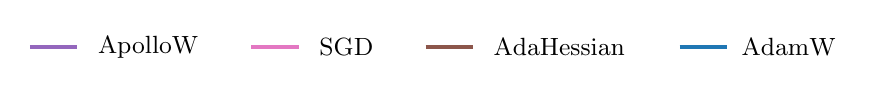
\begin{tikzpicture}[scale=0.75] % Nested TikZ environment
        \small 
        % AdaBelief
 \draw[mediumpurple148103189,  ultra thick] (0,0) -- ++(0.8,0);
 \node[anchor=west] at (1,0) {{ApolloW}}; % Increased spacing
 
 % Adam

 \draw[orchid227119194,  ultra thick] (3.75,0) -- ++(0.8,0);
 \node[anchor=west] at (4.75,0) {{SGD}}; % Increased spacing
 
 % AdaHessian
 \draw[sienna1408675,  ultra thick] (6.7,0) -- ++(0.8,0);
 \node[anchor=west] at (7.7,0) {{AdaHessian}}; % Increased spacing
 
 % Apollo
 \draw[steelblue31119180,  ultra thick] (11,0) -- ++(0.8,0);
 \node[anchor=west] at (11.9,0) {{AdamW}}; % Increased spacing
    
\end{tikzpicture}
};
    \end{tikzpicture}
     \\ % Replace with the correct path to your .tex file
    \end{tabular}
    \caption{Evaluation of optimizers on CIFAR-10 using ResNet-110 with the \emph{milestone} learning rate scheduler, where hyperparameters
    are choosen optimally across all optimizers.For better visualization we applied a polynomial transformation, with $\hat{x}=x^\alpha$ and $\alpha=5$, for every $x \in \mathcal{D}$ in the output data $ \mathcal{D}$.
    }
    \label{fig:cifar-10-milestone-second-best}
\end{figure}

The CIFAR-10 dataset comprises 60,000 RGB images, each with dimensions of 32x32 pixels,
categorized into 10 different classes, with 6,000 images per class and a training/test split of 50000/10000.
For evaluation, we utilize the ResNet-110 architecture.
Unlike ResNet-18, ResNet-110 is specifically designed to handle smaller images,
such as those found in the CIFAR-10 dataset. ResNet-110 comprises 54 BasicBlocks,
divided into 3 layer groups, each containing 18 blocks. Each block in ResNet-110 is two layers deep.
The first layer consists of a 3x3 convolution, followed by batch normalization and an
activation function. The second layer also applies a 3x3 convolution and includes a
skip connection that directly adds the input of the block to the output of the second
layer. This is then followed by another application of an activation function (ReLU).
After each layer group, the channel width doubles. This results in 16 channels for the first block group and 32 and 64 channels
for the second and third block groups, respectively.
Together with the fully connected classification layer of size 64x10, where 10 corresponds to the number of classes,
this totals 110 layers \cite{Resnet110}.
Given Apollo's status as a recent advancement in the development of second-order optimizers,
we closely adhere to their evaluation methodology. This allows us to effectively compare their results
with our own in subsequent analyses. We therefore set our training batch size to 128. 
For the milestone lr-scheduler, we choose milestone epochs of $80$ and $120$ with
$\gamma=0.1$, meaning that the learning rate is decayed by a factor of $10^{-1}$ at 
epochs $80$ and $120$. For both the cosine-annealing and milestone learning rate scheduler, we train the model
for $164$ epochs. 
To ensure a fair comparison between first and second-order optimizers, we employed two key strategies.
First, we addressed the potential for inherent advantages due to superior hyperparameter settings.
To mitigate this, we applied the optimal hyperparameters of Adam or AdamW—widely regarded as industry
standards—to the second-order optimizers.
The authors of Apollo \cite{apollo} note that both Apollo(W) and AdaHessian benefit significantly
from learning rate warmup. However, our goal was to evaluate the real-world applicability of
these second-order optimizers under basic conditions. Therefore, we opted for the most
rudimentary settings to assess whether Apollo(W) and AdaHessian could perform well
without such enhancements.
This approach tests the optimizers' effectiveness in real-world conditions,
where complex tuning is often impractical. Secondly, we test all optimizers with their
respective optimal parameters as mentioned in \cite{apollo}.
As discussed in Section~\ref{sec:dcp_weightdecay}, \emph{weight decay} introduces
an additional constraint to the optimizer. This technique aids in regularization,
though it can sometimes result in slower convergence.
To ensure fairness in our comparison, we applied the same learning rate and weight decay across all optimizers,
which are listed in \ref{tab:cifar-real-comp}.

Examining the results presented in Figure~\ref{fig:cifar-10-milestone-real}, which utilizes milestone
learning rate decay, we observe several key findings. \emph{AdamW} and \emph{AdaBelief} converge the fastest with the best generalization.
Although not optimally tuned, \emph{Apollo(W)} shows reasonable convergence and generalization,
while \emph{AdaHessian} performs poorly with the chosen hyperparameters.
When optimally tuned however, as shown in Figure~\ref{fig:cifar-10-milestone-second-best}, \emph{Apollo(W)} and \emph{AdaHessian} are capable of 
outperforming other optimizers by a small margin. This suggests that \emph{AdaHessian} may require additional effort to tune its hyperparameters optimally,
as commonly used settings from first-order methods have a much worse impact on performance compared to \emph{Apollo(W)}.



%As a tradeoff, \emph{AdaHessian} converges slower than all other optimizers.
%In contrast, \emph{ApolloW} matches the convergence speed of \emph{Adam} and \emph{AdaBelief}.

\begin{figure}[h!]
    \centering
    \begin{tabular}{cc}
        % This file was created with tikzplotlib v0.10.1.
\begin{tikzpicture}[scale=0.75]

\definecolor{crimson2143940}{RGB}{214,39,40}
\definecolor{darkgrey176}{RGB}{176,176,176}
\definecolor{darkorange25512714}{RGB}{255,127,14}
\definecolor{forestgreen4416044}{RGB}{44,160,44}
\definecolor{grey127}{RGB}{127,127,127}
\definecolor{lightgrey204}{RGB}{204,204,204}
\definecolor{mediumpurple148103189}{RGB}{148,103,189}
\definecolor{orchid227119194}{RGB}{227,119,194}
\definecolor{sienna1408675}{RGB}{140,86,75}
\definecolor{steelblue31119180}{RGB}{31,119,180}

\begin{groupplot}[group style={group size=2 by 2,
    horizontal sep=1cm,  % Adjust horizontal spacing
    vertical sep=2cm}]
\nextgroupplot[
tick align=outside,
tick pos=left,
title={Polynom. Training Accuracy (cosine)},
x grid style={darkgrey176},
xlabel={Epochs},
xmin=-8.15, xmax=171.15,
xtick style={color=black},
y grid style={darkgrey176},
ymin=-0.0499822733918491, ymax=1.0499991558758,
ytick style={color=black}
]
\addplot [semithick, steelblue31119180]
table {%
0 0.00351974889468086
1 0.0207733636198212
2 0.0443754516206132
3 0.0791368466986102
4 0.119562218868269
5 0.16286674400272
6 0.199405307362081
7 0.235616950132586
8 0.264360457034578
9 0.297631712698064
10 0.323997304937945
11 0.348811267695195
12 0.365569617617929
13 0.391115880998462
14 0.410570921544399
15 0.424675602012245
16 0.442913621443509
17 0.457231762476172
18 0.480507418411895
19 0.490416468557669
20 0.50285249367647
21 0.513638577137534
22 0.534408170991427
23 0.545348208340006
24 0.552740564114306
25 0.564766398816591
26 0.586923659543573
27 0.587980359208041
28 0.596571154460558
29 0.612035453544056
30 0.623885427046819
31 0.625849638925886
32 0.630996965381877
33 0.648048073426368
34 0.65911360750626
35 0.669066033834322
36 0.677405687363377
37 0.682247673014658
38 0.694148663668485
39 0.70320638928537
40 0.71492277311573
41 0.712453266761618
42 0.721126508668236
43 0.740876924703436
44 0.743817531152537
45 0.750913094538574
46 0.761757933859391
47 0.756469216016943
48 0.768082957745844
49 0.775870525403044
50 0.782084629567802
51 0.787310531526576
52 0.790397616476456
53 0.792254510525118
54 0.806606950684575
55 0.814705137878666
56 0.806921253947683
57 0.810069678694476
58 0.824466040245088
59 0.823081135332205
60 0.822868238322058
61 0.837661863321439
62 0.83679849472952
63 0.85529898140745
64 0.84470318378557
65 0.853434343028759
66 0.850151738801624
67 0.869666002803669
68 0.866888229417073
69 0.86135397639176
70 0.877705797114915
71 0.873678501574088
72 0.877369623001538
73 0.889083938735535
74 0.885353427016513
75 0.892486215251525
76 0.894191254902508
77 0.888970708483678
78 0.893963765841966
79 0.897837382756668
80 0.890783777522225
81 0.904935600155009
82 0.913350652501634
83 0.905280197495642
84 0.913003599618129
85 0.913119272188564
86 0.915203384084665
87 0.91531927955915
88 0.92194475654007
89 0.917871951977367
90 0.923811418727743
91 0.932248852801412
92 0.923577920746242
93 0.936018556140623
94 0.929898962757199
95 0.931660935426449
96 0.936254566869665
97 0.938617293590669
98 0.943238330204835
99 0.944426138050971
100 0.941340323767005
101 0.943594546997596
102 0.948592892553841
103 0.945734108479494
104 0.949189341788349
105 0.945615142228704
106 0.950980489866686
107 0.956730342541923
108 0.959856438115074
109 0.957931721594023
110 0.957691349287296
111 0.961543101788266
112 0.968798537714328
113 0.965649157787999
114 0.962387322300209
115 0.966859486972427
116 0.96069947383055
117 0.964802648785247
118 0.968555986381681
119 0.970983687154153
120 0.975487766027397
121 0.968434728934492
122 0.973051058115229
123 0.970862186617848
124 0.976219729501627
125 0.974756241676348
126 0.981846059289563
127 0.978296012424459
128 0.978540513076147
129 0.981478335868823
130 0.980375826616374
131 0.984054715082111
132 0.978418256640383
133 0.978662781732667
134 0.985652325867234
135 0.986390384185179
136 0.986636501850549
137 0.984300366423927
138 0.984054715082111
139 0.98466893541793
140 0.990457612105862
141 0.99021073217187
142 0.98910038160839
143 0.995033780184654
144 0.99132207968303
145 0.989717119992471
146 0.991692750513346
147 0.993424014089807
148 0.992805428332213
149 0.993547768233472
150 0.992434424813065
151 0.994414392610996
152 0.994909877985751
153 0.99305282564679
154 0.994414392610996
155 0.9945382454434
156 0.995033780184654
157 0.995157694727487
158 0.996521569661856
159 0.996893794956395
160 0.996025442234843
161 0.996025442234843
162 0.997638579230178
163 0.99801113825927
};
\addplot [semithick, darkorange25512714]
table {%
0 0.00436636353751514
1 0.0220839439207118
2 0.0467509757895655
3 0.0909709803146828
4 0.131842947956887
5 0.17100552340898
6 0.207230861567133
7 0.239874265160676
8 0.267637969138665
9 0.293876274096392
10 0.31451589530295
11 0.334689537571092
12 0.354038385732064
13 0.372179703229884
14 0.388831742391435
15 0.403540141194307
16 0.421674461414814
17 0.432762262590652
18 0.44084242298771
19 0.465337318857348
20 0.467364634920983
21 0.480092281282209
22 0.491754633102719
23 0.510143855801029
24 0.513200692613015
25 0.526318944039262
26 0.529303449817354
27 0.539628143204597
28 0.549188457146646
29 0.566264493911426
30 0.560525958400183
31 0.575559823091655
32 0.580293283723352
33 0.598631306497646
34 0.599209167774228
35 0.606095031383265
36 0.612455542107934
37 0.614138203717856
38 0.62286258043188
39 0.642527657151727
40 0.641131655056741
41 0.643838616597144
42 0.647257127946933
43 0.668254629533727
44 0.670420125693335
45 0.673860306000794
46 0.68151503846335
47 0.687578137834287
48 0.678682022006496
49 0.707346095955992
50 0.693777163188014
51 0.707817748044918
52 0.711031658812851
53 0.709234214081334
54 0.729207354665886
55 0.726602080432741
56 0.732595678896124
57 0.745094690074016
58 0.7405833763456
59 0.742346063085608
60 0.758561220314021
61 0.752695418186592
62 0.755275858917569
63 0.767076190519783
64 0.764664255975651
65 0.764764631960807
66 0.779431145173419
67 0.781267404320972
68 0.788955774076572
69 0.79546067455651
70 0.777394908381923
71 0.801070389089789
72 0.808074537605489
73 0.811331796879108
74 0.80305168692282
75 0.811647572094617
76 0.815761604796494
77 0.814282857714688
78 0.819998437916681
79 0.825746068006901
80 0.82788298024275
81 0.835612525450544
82 0.831525882585642
83 0.84481188040677
84 0.837338016629526
85 0.843942620667794
86 0.845790653624204
87 0.851572958149337
88 0.847859931854063
89 0.853763160325416
90 0.856727079262581
91 0.865889970391967
92 0.863343041533708
93 0.866777266303524
94 0.877593727629487
95 0.879612730750179
96 0.872562436083368
97 0.878378454483076
98 0.883436541384072
99 0.878714937785234
100 0.881522977401553
101 0.885804942129143
102 0.886030768754388
103 0.902755586409514
104 0.898408163019692
105 0.890670374113394
106 0.903328866457583
107 0.905739823906503
108 0.906429613545437
109 0.907349986738127
110 0.909538869639526
111 0.907925599530919
112 0.919150422094848
113 0.919732015610833
114 0.916826989456715
115 0.920197502361735
116 0.925798058953717
117 0.935428737540029
118 0.932484102838772
119 0.927319559316287
120 0.929664234627652
121 0.940866299895784
122 0.937907975299553
123 0.938735555017491
124 0.938972113632074
125 0.945139396940008
126 0.94490159611169
127 0.943475796110886
128 0.950980489866686
129 0.951697705749795
130 0.958532863525988
131 0.960217666636541
132 0.952894027131432
133 0.95086099593717
134 0.953732167684466
135 0.959254632171401
136 0.964681767405092
137 0.966738399470453
138 0.969041137637414
139 0.967707439261759
140 0.964802648785247
141 0.967949820585342
142 0.975000034347433
143 0.974146973349223
144 0.973051058115229
145 0.973416253544139
146 0.973294509553404
147 0.980620743007421
148 0.983072600122528
149 0.97939665035895
150 0.982459176579853
151 0.983563559535474
152 0.981478335868823
153 0.984423210490172
154 0.987621463838396
155 0.985529359111827
156 0.987498300589206
157 0.985652325867234
158 0.988237464432872
159 0.988360701427909
160 0.989963901469861
161 0.991939925993913
162 0.992805428332213
163 0.993547768233472
};
\addplot [semithick, forestgreen4416044]
table {%
0 0.00457307733953142
1 0.0254331485209618
2 0.0534947572064631
3 0.0910075442130507
4 0.131523501593613
5 0.175565985977862
6 0.206138320345017
7 0.241466574380119
8 0.273848823067992
9 0.301139581238457
10 0.322938260393763
11 0.349079188344113
12 0.372913740708696
13 0.395538622794051
14 0.412160147566384
15 0.431490667482251
16 0.44950195832362
17 0.466485265597242
18 0.479470113624302
19 0.492318943951417
20 0.506884855471748
21 0.523051552832704
22 0.538717404232188
23 0.547419265033563
24 0.561074203622721
25 0.568003100197951
26 0.586274138335098
27 0.585463045603155
28 0.608683036703583
29 0.612539587494528
30 0.625849638925886
31 0.647520690582067
32 0.647344972620936
33 0.650778361793968
34 0.667894258183128
35 0.687393775819572
36 0.684724967694026
37 0.696846804211361
38 0.696008553989295
39 0.719691069659022
40 0.72640939378596
41 0.72814504609746
42 0.733566081280594
43 0.742934370595159
44 0.747358576205002
45 0.762458649407267
46 0.777598340345111
47 0.772424109561996
48 0.77871797754158
49 0.779635003294701
50 0.786283649533217
51 0.802842944835902
52 0.798157711559053
53 0.80023732927308
54 0.813966262517228
55 0.824466040245088
56 0.831418555686799
57 0.838093814769426
58 0.833459662872224
59 0.83712217448585
60 0.839715220018862
61 0.844268509177488
62 0.855628373293478
63 0.850916774769416
64 0.867887408920689
65 0.862679611973718
66 0.879388213744164
67 0.874348688840801
68 0.874683936666224
69 0.878266316291663
70 0.896924737783475
71 0.888291569213291
72 0.898179816090459
73 0.901380901745564
74 0.88965026307683
75 0.896924737783475
76 0.907925599530919
77 0.905969707109355
78 0.905395086601222
79 0.909654190911045
80 0.923111066425936
81 0.918801607234438
82 0.917523525326198
83 0.926968266427359
84 0.926266000038928
85 0.9275538137382
86 0.919848369634368
87 0.930603431636047
88 0.932837066939466
89 0.94490159611169
90 0.935546677466946
91 0.93814436706549
92 0.934485646261958
93 0.937907975299553
94 0.938853828364326
95 0.946210093224232
96 0.943713309841301
97 0.943950871403304
98 0.95002487472022
99 0.947758367388378
100 0.961181474409778
101 0.960338100308361
102 0.957931721594023
103 0.957210749432834
104 0.958532863525988
105 0.958532863525988
106 0.963835936958132
107 0.96371515248537
108 0.96069947383055
109 0.963956733541131
110 0.968434728934492
111 0.972442642646359
112 0.964681767405092
113 0.965165365634496
114 0.969647850076219
115 0.97707424215485
116 0.976952132296705
117 0.973294509553404
118 0.980375826616374
119 0.975975692873219
120 0.973538009717193
121 0.978051560648462
122 0.978540513076147
123 0.976463814943462
124 0.983195321591444
125 0.983440801296999
126 0.984423210490172
127 0.976219729501627
128 0.978785062610857
129 0.982704509240213
130 0.984914709412167
131 0.9845460668212
132 0.988360701427909
133 0.99132207968303
134 0.988360701427909
135 0.986882668641202
136 0.987744639376262
137 0.986882668641202
138 0.989963901469861
139 0.990457612105862
140 0.98910038160839
141 0.993671534710002
142 0.992063532215067
143 0.989470387732338
144 0.990334165984407
145 0.9945382454434
146 0.9945382454434
147 0.993424014089807
148 0.992929120825373
149 0.993671534710002
150 0.995157694727487
151 0.996645632403804
152 0.996273481242038
153 0.996397519274908
154 0.995901441258672
155 0.996273481242038
156 0.997762753208669
157 0.998259572774184
158 0.997390268362198
159 0.997266131470862
160 0.998756590226503
161 0.997514417614995
162 0.998135349333226
163 0.998259572774184
};
\addplot [semithick, crimson2143940]
table {%
0 0.00100507479246187
1 0.00995096306871792
2 0.0384972173008099
3 0.0879768789358813
4 0.151654587919203
5 0.216175548707324
6 0.255220369068115
7 0.300758765528946
8 0.327547537347653
9 0.361252045453887
10 0.382389084154745
11 0.405711717552009
12 0.429462334066696
13 0.444277070827815
14 0.465472253995006
15 0.480784336003901
16 0.494298113031665
17 0.509853489905089
18 0.522681287562106
19 0.536294777263708
20 0.542978063536198
21 0.562957159236231
22 0.575000282169363
23 0.58912004500263
24 0.593368646375015
25 0.596818072790469
26 0.607012346205004
27 0.613464695855163
28 0.620990846125748
29 0.628504879376999
30 0.6360048526703
31 0.651837714826797
32 0.65635536711816
33 0.654137712619454
34 0.661612884316472
35 0.67795245257975
36 0.68151503846335
37 0.682156059254482
38 0.685368402483725
39 0.693034639401876
40 0.710179783920142
41 0.704427461715779
42 0.709423247427119
43 0.710652946885995
44 0.722660167213553
45 0.723523996141183
46 0.73249869516901
47 0.735704586412962
48 0.73152942269707
49 0.733857402428575
50 0.732207805613549
51 0.745094690074016
52 0.75656873048955
53 0.75896022155197
54 0.770705500466329
55 0.768284437981278
56 0.762358515628065
57 0.772221761277784
58 0.769393335190425
59 0.768183692579111
60 0.788441340606375
61 0.781675931505261
62 0.771918318365882
63 0.798053844281129
64 0.794218349834946
65 0.796600837433481
66 0.81049021010767
67 0.801591403686015
68 0.810174795179165
69 0.798157711559053
70 0.806921253947683
71 0.82457264855676
72 0.811858143522228
73 0.825639338342582
74 0.830238691063881
75 0.82169809209094
76 0.824466040245088
77 0.837985810205692
78 0.846443672936515
79 0.847859931854063
80 0.842314687289266
81 0.844159868490327
82 0.843508259205699
83 0.859368579042788
84 0.864560389114517
85 0.848841528829664
86 0.863121853012238
87 0.858817730015311
88 0.867998485712839
89 0.855408767429102
90 0.879163742586017
91 0.884112709743086
92 0.887725936944379
93 0.876585617312134
94 0.87950046651575
95 0.88783904034054
96 0.881972929145439
97 0.892599803579949
98 0.893167918714412
99 0.899207743035815
100 0.904246720286309
101 0.895671062903237
102 0.906084666213246
103 0.907349986738127
104 0.910692608829004
105 0.901037492384364
106 0.91462408279166
107 0.924044963933022
108 0.924629033597267
109 0.918336685494573
110 0.92171163609104
111 0.931308327401035
112 0.936962884712013
113 0.937907975299553
114 0.93236647188438
115 0.937435334724951
116 0.938972113632074
117 0.94252621936065
118 0.942763541836939
119 0.949308667630074
120 0.948712158407209
121 0.948592892553841
122 0.95421136986933
123 0.959856438115074
124 0.949428005472185
125 0.956490211439639
126 0.960217666636541
127 0.965165365634496
128 0.963473619866913
129 0.971834531552624
130 0.970740698244671
131 0.968677255974656
132 0.981478335868823
133 0.977562803694235
134 0.978296012424459
135 0.980375826616374
136 0.983563559535474
137 0.983809112788409
138 0.984054715082111
139 0.988730486181861
140 0.987867827203724
141 0.987375149627771
142 0.992063532215067
143 0.995901441258672
144 0.997142006940065
145 0.993919104665349
146 0.995653476356568
147 0.995901441258672
148 0.996769707501676
149 0.997886939551392
150 0.998259572774184
151 0.999129483214514
152 0.997886939551392
153 0.998508056760799
154 0.99937814041027
155 0.999005173178685
156 0.999129483214514
157 0.998756590226503
158 0.998880875516322
159 0.99937814041027
160 0.999502487572043
161 0.999751219028001
162 1
163 0.999875603324033
};
\addplot [semithick, mediumpurple148103189]
table {%
0 0.00141657909787913
1 0.0132378359470608
2 0.0426031762643852
3 0.0951398607175928
4 0.152785921712018
5 0.207230861567133
6 0.249883469882105
7 0.282429399485147
8 0.318929144890459
9 0.341692042672669
10 0.362963091039523
11 0.38169772819006
12 0.411915331471864
13 0.423923719993734
14 0.44252467996228
15 0.461169824807106
16 0.472259032177343
17 0.488169303689504
18 0.496354671734164
19 0.511597670348833
20 0.524608959087029
21 0.537126570136932
22 0.552121489792064
23 0.549496609117984
24 0.556933856268533
25 0.568874003285122
26 0.587004890154839
27 0.589690550232803
28 0.601359417911047
29 0.602519799054115
30 0.609519760296291
31 0.627390296481407
32 0.617853078903997
33 0.61810701895382
34 0.638607586351395
35 0.642964406134441
36 0.648048073426368
37 0.657155193483348
38 0.664030075845251
39 0.665016880701339
40 0.66447847818145
41 0.668705312452895
42 0.669878226118523
43 0.675676591046714
44 0.682522573354796
45 0.696753625434155
46 0.697126400357639
47 0.701612157869256
48 0.696753625434155
49 0.703300257773007
50 0.706309346360079
51 0.717303751653954
52 0.713687165438359
53 0.717589894841493
54 0.721413871122214
55 0.732207805613549
56 0.73152942269707
57 0.722756107440598
58 0.742542124163426
59 0.748344589282477
60 0.747752856637378
61 0.745389668041526
62 0.751209913772191
63 0.758860455505686
64 0.754381829828784
65 0.751308874371945
66 0.766975571889548
67 0.760058340753283
68 0.769090781778836
69 0.775464427416394
70 0.769494207484278
71 0.784233099993084
72 0.772424109561996
73 0.785052805793064
74 0.781675931505261
75 0.789676432015616
76 0.793494377535864
77 0.797430867669518
78 0.805664628484743
79 0.801591403686015
80 0.800133245545882
81 0.811542302766844
82 0.812384763301296
83 0.8247858982643
84 0.821166647696709
85 0.815655908812599
86 0.815655908812599
87 0.823294076405582
88 0.837553903292801
89 0.830238691063881
90 0.832384896853854
91 0.836582763854715
92 0.836474915103556
93 0.836151435584725
94 0.842965558899922
95 0.848841528829664
96 0.85529898140745
97 0.848405151330755
98 0.864006879190603
99 0.86223755222796
100 0.871670405145048
101 0.859809461743872
102 0.869999813543154
103 0.870779103902994
104 0.872004831211581
105 0.87680956172435
106 0.867776343500328
107 0.880174223895724
108 0.87680956172435
109 0.889083938735535
110 0.875131093722808
111 0.890103530301187
112 0.890556982254536
113 0.903099519500008
114 0.909308262184096
115 0.916246866095489
116 0.9157829788731
117 0.913003599618129
118 0.917639655784399
119 0.914739919575979
120 0.920197502361735
121 0.91254102655626
122 0.917871951977367
123 0.928843059426256
124 0.930485990516606
125 0.923461189462172
126 0.933190137915312
127 0.928374077052432
128 0.93354331579058
129 0.931073314702273
130 0.943357057180266
131 0.95265466666363
132 0.953492638799097
133 0.959254632171401
134 0.94883143625644
135 0.95086099593717
136 0.959134307213301
137 0.963232135678477
138 0.965649157787999
139 0.961422547237039
140 0.966254170774487
141 0.967465106495774
142 0.966859486972427
143 0.973659778073478
144 0.973659778073478
145 0.978907355711635
146 0.97451249777477
147 0.983563559535474
148 0.988114239731109
149 0.982091269462733
150 0.983809112788409
151 0.989347040056443
152 0.988853772359191
153 0.987498300589206
154 0.993919104665349
155 0.993424014089807
156 0.995157694727487
157 0.995777452632888
158 0.994166723963222
159 0.99429055211791
160 0.997390268362198
161 0.998259572774184
162 0.998508056760799
163 0.998383808583067
};
\addplot [semithick, sienna1408675]
table {%
0 6.98568764883273e-05
1 0.000439223132033488
2 0.00269083126505947
3 0.00613886224084626
4 0.0117563375430031
5 0.0170325599683166
6 0.0243572232866694
7 0.0334639218486803
8 0.0442931682173064
9 0.0573169376772375
10 0.0698306270003313
11 0.0847335116764876
12 0.097957744229501
13 0.117618820571445
14 0.135423131166422
15 0.152675251388381
16 0.170581943056688
17 0.191419896512687
18 0.202784163228209
19 0.224709605867886
20 0.245201392083041
21 0.262819200556857
22 0.276151847159954
23 0.290020171311251
24 0.308740089117191
25 0.321982465228761
26 0.340166728128422
27 0.353550774403487
28 0.369255103147225
29 0.37837025674013
30 0.400958511016918
31 0.408378551647696
32 0.415414964634005
33 0.434611398780957
34 0.448387577887064
35 0.445578713761689
36 0.460433559634734
37 0.473010384260486
38 0.477400878372407
39 0.495786662785599
40 0.497492251435988
41 0.52216326848731
42 0.523273812696137
43 0.533278758274794
44 0.541377169004296
45 0.542901744690068
46 0.54826483061995
47 0.570222045342076
48 0.575799759649555
49 0.583115951897379
50 0.60061440316884
51 0.601525077097918
52 0.605511863235955
53 0.611447716849871
54 0.621330826324067
55 0.617091759485283
56 0.620735958656427
57 0.644276078270804
58 0.635485325780326
59 0.648048073426368
60 0.65848997001039
61 0.665016880701339
62 0.666814076854824
63 0.681698138066942
64 0.683347806097316
65 0.68454121797211
66 0.703581923382322
67 0.704709488401047
68 0.707723397505457
69 0.72179716355631
70 0.72679480796685
71 0.732692672895577
72 0.735607273566029
73 0.7405833763456
74 0.749035417441998
75 0.747555695625809
76 0.752001890627847
77 0.757763721269992
78 0.757564451352019
79 0.769796887847455
80 0.782800262514264
81 0.781063204791423
82 0.792048016791905
83 0.791531970826276
84 0.791016193872769
85 0.806921253947683
86 0.790809958391197
87 0.812595487714797
88 0.806397469592164
89 0.825425912122101
90 0.825532619714601
91 0.826279881903524
92 0.830345896101063
93 0.822442576464105
94 0.835397039215823
95 0.85409207896553
96 0.854421098972526
97 0.846770333812886
98 0.862127065611981
99 0.869888531909436
100 0.875242911556369
101 0.867665289450883
102 0.876921551092702
103 0.867776343500328
104 0.887725936944379
105 0.884676499586591
106 0.886369595048228
107 0.894532575325625
108 0.898293983750481
109 0.901266420326571
110 0.906314619430398
111 0.898750770491308
112 0.901380901745564
113 0.916362867268471
114 0.91822048447163
115 0.918917867085894
116 0.926266000038928
117 0.935192893369698
118 0.927788115498583
119 0.940155622158088
120 0.94157740733809
121 0.943357057180266
122 0.94311961518369
123 0.952774340884204
124 0.954331200507114
125 0.951578139728318
126 0.957691349287296
127 0.961302004777847
128 0.96069947383055
129 0.962870000186177
130 0.962749312562531
131 0.973294509553404
132 0.969283786158242
133 0.974756241676348
134 0.974634363629828
135 0.977440644991537
136 0.978785062610857
137 0.981723472571698
138 0.980375826616374
139 0.982581836784526
140 0.985283462419244
141 0.989963901469861
142 0.991075027379098
143 0.9845460668212
144 0.99021073217187
145 0.991075027379098
146 0.991445624308958
147 0.986882668641202
148 0.991816332093646
149 0.990087310667327
150 0.99132207968303
151 0.99218715075803
152 0.993671534710002
153 0.995405560848633
154 0.996893794956395
155 0.995653476356568
156 0.9945382454434
157 0.996893794956395
158 0.996769707501676
159 0.996025442234843
160 0.995157694727487
161 0.996273481242038
162 0.997762753208669
163 0.998383808583067
};
\addplot [semithick, orchid227119194]
table {%
0 1.68824839532658e-05
1 5.82294747267606e-05
2 0.000130953607750532
3 0.00036838696198446
4 0.000564260102005105
5 0.00076855698666369
6 0.00152789242698375
7 0.00277271438018744
8 0.00395002649430071
9 0.00511695101288593
10 0.00819709528043541
11 0.0123217575858721
12 0.0192445175517386
13 0.0302597963635055
14 0.0458036400051973
15 0.0565255570294529
16 0.0795300399288114
17 0.101878398712817
18 0.123269472179143
19 0.146472210119696
20 0.171247946850906
21 0.197562828885815
22 0.216212083361408
23 0.245201392083041
24 0.265176808103648
25 0.285930397307004
26 0.302858028558428
27 0.323997304937945
28 0.341007605827138
29 0.358451144640452
30 0.37455538284712
31 0.39035331202234
32 0.400061057386134
33 0.421549783120717
34 0.435314446484867
35 0.45246248729722
36 0.469602837266506
37 0.471781396369306
38 0.495786662785599
39 0.510724984470929
40 0.51781340670473
41 0.528780186364228
42 0.531250627759393
43 0.546574743033065
44 0.568715577864672
45 0.565712194739687
46 0.577882563582394
47 0.592877175960496
48 0.601442242941623
49 0.605845047184327
50 0.619802087231853
51 0.625165874499872
52 0.648663787659843
53 0.647608563870748
54 0.654758050720499
55 0.669156238498193
56 0.678134786087538
57 0.686472558851833
58 0.69294186864818
59 0.709423247427119
60 0.709517779213813
61 0.703581923382322
62 0.717113040246
63 0.723427974376734
64 0.735315396807895
65 0.745291331673848
66 0.746964462109356
67 0.750418604318577
68 0.758760699951151
69 0.768889132387764
70 0.780246833600941
71 0.772626500261674
72 0.783516419226874
73 0.790088472931254
74 0.797742307325547
75 0.806711707554832
76 0.815127593217198
77 0.813544288777623
78 0.813438822692466
79 0.820423087538808
80 0.827562161689623
81 0.831418555686799
82 0.828417898929172
83 0.850698136888104
84 0.851463566150131
85 0.851135457602104
86 0.856507247825973
87 0.857826913614
88 0.860802109433728
89 0.860691769993589
90 0.878490604128558
91 0.872562436083368
92 0.882760786794564
93 0.890103530301187
94 0.889310433853006
95 0.900350987660155
96 0.900007892249288
97 0.893054272552263
98 0.904017186915164
99 0.894987831347201
100 0.901266420326571
101 0.907465085934592
102 0.916246866095489
103 0.924512196043574
104 0.921012557671419
105 0.91822048447163
106 0.922177924155605
107 0.930603431636047
108 0.93472134773786
109 0.930955826145651
110 0.932601745665484
111 0.940629359581214
112 0.940984787956975
113 0.944307303446339
114 0.943713309841301
115 0.947758367388378
116 0.957931721594023
117 0.952894027131432
118 0.958653128119388
119 0.955890094626591
120 0.963473619866913
121 0.964077542235277
122 0.963835936958132
123 0.960579003904457
124 0.962146055956741
125 0.968192250473821
126 0.973294509553404
127 0.974634363629828
128 0.973538009717193
129 0.976830034647409
130 0.97707424215485
131 0.97707424215485
132 0.979886140640976
133 0.981110722632887
134 0.980130959163337
135 0.981478335868823
136 0.9845460668212
137 0.987128884564491
138 0.988853772359191
139 0.988730486181861
140 0.987375149627771
141 0.988977070834394
142 0.98577530489661
143 0.987867827203724
144 0.989470387732338
145 0.991692750513346
146 0.990087310667327
147 0.990704541279201
148 0.991075027379098
149 0.993300272278086
150 0.993176542797388
151 0.99305282564679
152 0.995529512428791
153 0.99255808032698
154 0.991939925993913
155 0.994166723963222
156 0.994414392610996
157 0.994909877985751
158 0.996645632403804
159 0.9945382454434
160 0.996645632403804
161 0.997017894768884
162 0.995529512428791
163 0.996025442234843
};
\addplot [semithick, grey127]
table {%
0 0.00123495170832649
1 0.00829349913011493
2 0.0229634106699226
3 0.0493727248105744
4 0.0787940797484677
5 0.112957615813523
6 0.152398856132719
7 0.19224996142448
8 0.229459446433167
9 0.259673635987076
10 0.289696818068836
11 0.320878583732297
12 0.340902405270843
13 0.362023974815424
14 0.384816723358059
15 0.397913724035592
16 0.416339862514605
17 0.438778980230744
18 0.453915523019793
19 0.47808982806342
20 0.48620979872229
21 0.498631915929004
22 0.515539532042597
23 0.528929647960934
24 0.541453316349877
25 0.555377828362888
26 0.569032464009288
27 0.586274138335098
28 0.590751232521127
29 0.603848141579053
30 0.610525042950181
31 0.624653443482755
32 0.638607586351395
33 0.653163845640327
34 0.654846708854301
35 0.660898032937532
36 0.681972861259177
37 0.682156059254482
38 0.697406086242702
39 0.707346095955992
40 0.719404256356127
41 0.725735312416015
42 0.72814504609746
43 0.740681215457724
44 0.739703289510937
45 0.755474647109055
46 0.757763721269992
47 0.76848596049564
48 0.770806510361402
49 0.777496619040721
50 0.785975793966974
51 0.794218349834946
52 0.802112689340474
53 0.80859919317643
54 0.810910916151086
55 0.81607875849314
56 0.824679267896212
57 0.822017090777021
58 0.836690623729749
59 0.838201830469085
60 0.839174473024792
61 0.841014150192216
62 0.850807450210271
63 0.860912460189862
64 0.85529898140745
65 0.867776343500328
66 0.867998485712839
67 0.866222621164219
68 0.877705797114915
69 0.880848394127757
70 0.888517902834868
71 0.888404730257911
72 0.892940637958626
73 0.892940637958626
74 0.890103530301187
75 0.904131947773537
76 0.902297171963883
77 0.904017186915164
78 0.900350987660155
79 0.90976952387962
80 0.907810453608489
81 0.912772289645002
82 0.91810429521171
83 0.9157829788731
84 0.917755798001157
85 0.928022464604611
86 0.926148997032731
87 0.922877710072808
88 0.931660935426449
89 0.931896066772051
90 0.931308327401035
91 0.93838080649346
92 0.937553477001194
93 0.935310809507913
94 0.938735555017491
95 0.944782713648375
96 0.9464481574542
97 0.945139396940008
98 0.947400893593487
99 0.948473638695428
100 0.954570897898908
101 0.952894027131432
102 0.95181728378977
103 0.957210749432834
104 0.953612397225282
105 0.956370163971112
106 0.962870000186177
107 0.960819955843219
108 0.964560898141548
109 0.962387322300209
110 0.962990699912777
111 0.968071029458514
112 0.964560898141548
113 0.964319195960654
114 0.967707439261759
115 0.968071029458514
116 0.970012023380183
117 0.976097705086202
118 0.97731849850135
119 0.974025156250867
120 0.975731705050916
121 0.974146973349223
122 0.977562803694235
123 0.977562803694235
124 0.981355785881978
125 0.981846059289563
126 0.980008543786281
127 0.980253386773063
128 0.983931907804706
129 0.980498278694188
130 0.987375149627771
131 0.982336528625274
132 0.983931907804706
133 0.986759579104756
134 0.98577530489661
135 0.987498300589206
136 0.987991027321699
137 0.986267343772176
138 0.988360701427909
139 0.989470387732338
140 0.988730486181861
141 0.988853772359191
142 0.99021073217187
143 0.988977070834394
144 0.99218715075803
145 0.991939925993913
146 0.991816332093646
147 0.992434424813065
148 0.993919104665349
149 0.993919104665349
150 0.995157694727487
151 0.994909877985751
152 0.993919104665349
153 0.995033780184654
154 0.996521569661856
155 0.995777452632888
156 0.996273481242038
157 0.994042908146009
158 0.995281621615173
159 0.997017894768884
160 0.996769707501676
161 0.997266131470862
162 0.996149455562325
163 0.995653476356568
};

\nextgroupplot[
tick align=outside,
tick pos=left,
title={Polynom. Test Accuracy (cosine)},
x grid style={darkgrey176},
xlabel={Epochs},
xmin=-8.15, xmax=171.15,
xtick style={color=black},
y grid style={darkgrey176},
ymin=-0.0337863485385773, ymax=0.709920198702792,
ytick style={color=black}
]
\addplot [semithick, steelblue31119180]
table {%
0 0.00336159170164825
1 0.0281463358128148
2 0.0434947509542267
3 0.0404433271000987
4 0.0544802992171669
5 0.159684298870563
6 0.135032190676455
7 0.194438394284163
8 0.166318799674023
9 0.23607129782578
10 0.266957173316775
11 0.241035820060946
12 0.291584410814523
13 0.360522682837927
14 0.212460457873734
15 0.321526746595649
16 0.293044702925245
17 0.279934025650673
18 0.335554621989344
19 0.308543368846291
20 0.384448898436464
21 0.3530298958533
22 0.404395594032705
23 0.381051927832095
24 0.366608049943949
25 0.344203544654602
26 0.316826716730356
27 0.367264896496527
28 0.399215933139106
29 0.420013989604323
30 0.406292380542829
31 0.418795711072887
32 0.408434765891167
33 0.465003488957338
34 0.353879853075742
35 0.359229251920898
36 0.443450485196538
37 0.398279905572026
38 0.410107305690865
39 0.43360315631308
40 0.401093267860635
41 0.404395594032705
42 0.454514331638777
43 0.425654643174901
44 0.468986478661066
45 0.440655104232993
46 0.450114169097583
47 0.442178104292394
48 0.435608717903793
49 0.450114169097583
50 0.467655794924312
51 0.457118692979656
52 0.452439400928379
53 0.474877521886123
54 0.484371516543858
55 0.420746316503446
56 0.479741368490421
57 0.452439400928379
58 0.45166325849759
59 0.496521623248625
60 0.458948838687605
61 0.478115679140956
62 0.481915830050988
63 0.412025484313965
64 0.467124367939556
65 0.432603149459766
66 0.477304488830567
67 0.497358833529218
68 0.489037345504078
69 0.438883577852724
70 0.490692666156293
71 0.501561842013871
72 0.505227389679244
73 0.47326503603514
74 0.519236806802344
75 0.469786341713288
76 0.503532944958332
77 0.501843049588105
78 0.492906729861853
79 0.461836621141393
80 0.493739061198424
81 0.522133679807484
82 0.508914337128082
83 0.479470113624302
84 0.503532944958332
85 0.489312921596203
86 0.479741368490421
87 0.497638154444069
88 0.481915830050988
89 0.492629535666944
90 0.531785228508833
91 0.499596916686551
92 0.502124383278527
93 0.520973383200144
94 0.512050845840309
95 0.483551844715986
96 0.503250980050546
97 0.518947828177047
98 0.526211009122142
99 0.482460675478687
100 0.524460475048727
101 0.527088027275949
102 0.508061598819228
103 0.527088027275949
104 0.544575092696105
105 0.522424076730115
106 0.541877994857264
107 0.529432460479117
108 0.546680251245057
109 0.523296042837376
110 0.528845571654813
111 0.534737943225944
112 0.53948955562512
113 0.529726100217028
114 0.538298498455392
115 0.531785228508833
116 0.529432460479117
117 0.538893763794133
118 0.492906729861853
119 0.550001506663742
120 0.538893763794133
121 0.538893763794133
122 0.556386904614903
123 0.541877994857264
124 0.537406586856808
125 0.55944834161667
126 0.546379116377826
127 0.544274885926837
128 0.573392032546993
129 0.570269669942856
130 0.554861220262964
131 0.554861220262964
132 0.568402791352012
133 0.568092120835088
134 0.576528056743834
135 0.580941527379197
136 0.55914159288975
137 0.553643084135444
138 0.568713597770298
139 0.582524300872188
140 0.581257806513348
141 0.58062538593731
142 0.567471187327043
143 0.577156904913446
144 0.568092120835088
145 0.556998117238136
146 0.569024540134525
147 0.574331403303108
148 0.577471534705855
149 0.567781586174953
150 0.574958334149724
151 0.574331403303108
152 0.574644800328987
153 0.575272004810097
154 0.574644800328987
155 0.571204946917485
156 0.584428180828231
157 0.58315837537495
158 0.581574223384734
159 0.589849555374837
160 0.580309382142722
161 0.571204946917485
162 0.582841269142445
163 0.58379300190684
};
\addplot [semithick, darkorange25512714]
table {%
0 0.00742543246728036
1 0.0293741281321022
2 0.0442554102166867
3 0.0576956179239642
4 0.104409212895081
5 0.136812810340578
6 0.0944767084497267
7 0.181118856989679
8 0.142884346959259
9 0.212319081476113
10 0.169009986468666
11 0.2097871484388
12 0.264420540516993
13 0.288139539794056
14 0.194965899113112
15 0.258245882511968
16 0.206172612192649
17 0.292313827362421
18 0.309497547263983
19 0.33433338846112
20 0.315272314153943
21 0.3532422318846
22 0.3532422318846
23 0.315272314153943
24 0.374552547462951
25 0.35558467878987
26 0.395017625776103
27 0.331094140642284
28 0.383540680324987
29 0.355798243155354
30 0.373440984419364
31 0.414192007554225
32 0.405580253385898
33 0.411785320247101
34 0.35218157257425
35 0.412987261402947
36 0.37611318091434
37 0.411545268183997
38 0.356011910122021
39 0.40015371974261
40 0.423440259664723
41 0.371889231319193
42 0.432353436265397
43 0.425901256518903
44 0.459472812646799
45 0.417823125076211
46 0.468720099888742
47 0.394785426378705
48 0.408434765891167
49 0.453216609977071
50 0.439642104422143
51 0.462363230688863
52 0.378576111527225
53 0.422214034785844
54 0.444470497382198
55 0.430359879150972
56 0.464210148339872
57 0.479741368490421
58 0.4437053125
59 0.474877521886123
60 0.427136038411924
61 0.491522005684375
62 0.419770107373297
63 0.459210765880125
64 0.453994886742641
65 0.437117753586536
66 0.416609934475581
67 0.455294390376698
68 0.502124383278527
69 0.424669331923747
70 0.485466140993279
71 0.465532985018315
72 0.480555869777273
73 0.453735342451039
74 0.485466140993279
75 0.49235246619383
76 0.426641782461182
77 0.481371476971995
78 0.428373682570295
79 0.460784841525592
80 0.478115679140956
81 0.47784515992239
82 0.474339539023202
83 0.477304488830567
84 0.500718975564277
85 0.486014194833338
86 0.489037345504078
87 0.496242803835597
88 0.523586956796628
89 0.478115679140956
90 0.456857720907804
91 0.517504864361147
92 0.426641782461182
93 0.513481634167262
94 0.475415992770654
95 0.516640627973701
96 0.50948346516011
97 0.556692443819294
98 0.495407097046864
99 0.490692666156293
100 0.501561842013871
101 0.482188191200383
102 0.543974811567653
103 0.529432460479117
104 0.49014039534436
105 0.51577754659627
106 0.553947417397733
107 0.487936282469162
108 0.514054844239829
109 0.519236806802344
110 0.482733282927641
111 0.544274885926837
112 0.543375059904325
113 0.533555287616646
114 0.523878000122841
115 0.555776228672675
116 0.523005258201953
117 0.550001506663742
118 0.543075382512598
119 0.544274885926837
120 0.530019870229887
121 0.556386904614903
122 0.55914159288975
123 0.53503393455226
124 0.542177143571877
125 0.540981340897977
126 0.553034818885341
127 0.53948955562512
128 0.542775837355791
129 0.56654080521119
130 0.561291662396019
131 0.538298498455392
132 0.563139838808115
133 0.55091009926289
134 0.555166089057945
135 0.577156904913446
136 0.556386904614903
137 0.564065750871775
138 0.55547109184646
139 0.548791915078931
140 0.575899756828908
141 0.546379116377826
142 0.575585812354892
143 0.585700197281782
144 0.571829146340912
145 0.562215143049104
146 0.579677787315644
147 0.579677787315644
148 0.591131000808037
149 0.59049
150 0.574958334149724
151 0.580941527379197
152 0.584745977547647
153 0.585063912499649
154 0.593057343951948
155 0.599839131512188
156 0.583475619614735
157 0.584428180828231
158 0.586974427621711
159 0.591451709893807
160 0.588570333225214
161 0.592093545655287
162 0.587931554977186
163 0.602764536267924
};
\addplot [semithick, forestgreen4416044]
table {%
0 0.007415771484375
1 0.0378493458747471
2 0.059308254164165
3 0.0706913759633999
4 0.0823580170898464
5 0.125288857518143
6 0.13951891392525
7 0.207834615777238
8 0.165854287187662
9 0.110389378888786
10 0.254793007527975
11 0.167367758642997
12 0.2274310493473
13 0.263747372484302
14 0.198155022771498
15 0.281878986762001
16 0.297645867482689
17 0.271228127979608
18 0.389474903233349
19 0.381503464607842
20 0.341714437029492
21 0.389474903233349
22 0.381503464607842
23 0.369901704351605
24 0.371889231319193
25 0.417094872072304
26 0.409868036557539
27 0.392238432136463
28 0.392469432384552
29 0.379025300028548
30 0.411305328085472
31 0.437369665609343
32 0.427630752325058
33 0.401093267860635
34 0.446260034627646
35 0.369461187902448
36 0.426394826122317
37 0.381955429329792
38 0.425408144083083
39 0.420746316503446
40 0.40795790106767
41 0.421235101669691
42 0.447541800886051
43 0.479198981470177
44 0.410346686553879
45 0.440148371186088
46 0.477034336874151
47 0.403449861065241
48 0.472460437384154
49 0.469519599532052
50 0.433352981408416
51 0.457902324840689
52 0.49014039534436
53 0.470587295735613
54 0.4437053125
55 0.476224614864148
56 0.483551844715986
57 0.489312921596203
58 0.483551844715986
59 0.467124367939556
60 0.478927971986405
61 0.436362713888538
62 0.477034336874151
63 0.499596916686551
64 0.468453842170164
65 0.465797913867029
66 0.514915619070753
67 0.436362713888538
68 0.453216609977071
69 0.518947828177047
70 0.520104515176166
71 0.514341641177701
72 0.52504346796028
73 0.537109545858732
74 0.501843049588105
75 0.520104515176166
76 0.518658978229752
77 0.50834571781381
78 0.495407097046864
79 0.494016754701634
80 0.536812636222068
81 0.521843412036251
82 0.486288407303695
83 0.519236806802344
84 0.538001063111539
85 0.50834571781381
86 0.521553273373331
87 0.523296042837376
88 0.53948955562512
89 0.530019870229887
90 0.531196253897808
91 0.544875431919274
92 0.543674869574748
93 0.534737943225944
94 0.545175903640167
95 0.537406586856808
96 0.529726100217028
97 0.525335158768613
98 0.516065112125804
99 0.548489849963467
100 0.556692443819294
101 0.528259203410425
102 0.542775837355791
103 0.548489849963467
104 0.537406586856808
105 0.53948955562512
106 0.561291662396019
107 0.542177143571877
108 0.531785228508833
109 0.554251884476997
110 0.562831471802696
111 0.558528499096899
112 0.56437465872355
113 0.556386904614903
114 0.559755224956304
115 0.545476507902619
116 0.565302194392784
117 0.5668507968897
118 0.53503393455226
119 0.532374725434074
120 0.560676683094537
121 0.566230949166752
122 0.563756978298233
123 0.562831471802696
124 0.56437465872355
125 0.562831471802696
126 0.562523239897825
127 0.560062242952952
128 0.569646832879189
129 0.561599354342574
130 0.571829146340912
131 0.571829146340912
132 0.572141450618738
133 0.595311088045607
134 0.573079182252969
135 0.570269669942856
136 0.574644800328987
137 0.579677787315644
138 0.569958183348838
139 0.584110522296319
140 0.58062538593731
141 0.579993515950482
142 0.580941527379197
143 0.571829146340912
144 0.578101205930159
145 0.588889930488108
146 0.589849555374837
147 0.59821882146116
148 0.593700573114823
149 0.595956271780447
150 0.595633610027442
151 0.594344360273028
152 0.586655662326952
153 0.594988705789528
154 0.588570333225214
155 0.592735938505377
156 0.593378888806648
157 0.596279073350048
158 0.58825087473664
159 0.586018547202122
160 0.585381985729327
161 0.593378888806648
162 0.596925096120781
163 0.595956271780447
};
\addplot [semithick, crimson2143940]
table {%
0 0.00244188843130308
1 0.00898182719488627
2 0.0301370518509276
3 0.0355929364046007
4 0.0941812843270507
5 0.190648033756904
6 0.208669627219306
7 0.208390992425028
8 0.248959784943214
9 0.229981035610261
10 0.250730702292062
11 0.240566878918917
12 0.29616725209077
13 0.291766628288406
14 0.3936260667123
15 0.382407822302064
16 0.368361732701375
17 0.3803754244027
18 0.421479664541448
19 0.356439552006768
20 0.390394343105387
21 0.423194787057026
22 0.428869542781753
23 0.383087215395442
24 0.37034264089032
25 0.427383338103309
26 0.421969131059964
27 0.417580261141208
28 0.407243439069632
29 0.361603385547953
30 0.413468822989359
31 0.379025300028548
32 0.40015371974261
33 0.445492385667387
34 0.403686128253106
35 0.409628879114786
36 0.437117753586536
37 0.43360315631308
38 0.430608670842294
39 0.474877521886123
40 0.404632304160866
41 0.423440259664723
42 0.455034251890535
43 0.423440259664723
44 0.457379784298512
45 0.451404781190356
46 0.43410385274505
47 0.432603149459766
48 0.467655794924312
49 0.433853446745288
50 0.417337510153039
51 0.449083806318157
52 0.425654643174901
53 0.431355736364926
54 0.471121871729231
55 0.43185435581965
56 0.486288407303695
57 0.428621555311354
58 0.436111265978953
59 0.479470113624302
60 0.43435437435238
61 0.397112340986687
62 0.490416468557669
63 0.392238432136463
64 0.394321355163574
65 0.387183880751436
66 0.467921689729198
67 0.468986478661066
68 0.503250980050546
69 0.468453842170164
70 0.470854523040325
71 0.503250980050546
72 0.459734979028565
73 0.494572516547412
74 0.478386320863411
75 0.479198981470177
76 0.481915830050988
77 0.536515857903242
78 0.547584452587599
79 0.451146422233535
80 0.40015371974261
81 0.479198981470177
82 0.500438272030825
83 0.495685540776928
84 0.430111202467942
85 0.517504864361147
86 0.471121871729231
87 0.427630752325058
88 0.497079638053195
89 0.507493741942045
90 0.500999805044349
91 0.420746316503446
92 0.466328133406711
93 0.467124367939556
94 0.501280760513418
95 0.446772388229937
96 0.53090196235163
97 0.558222153942417
98 0.503815036236942
99 0.558834978731253
100 0.560676683094537
101 0.495407097046864
102 0.504097253928849
103 0.553643084135444
104 0.516640627973701
105 0.571516978455388
106 0.540981340897977
107 0.524460475048727
108 0.490692666156293
109 0.520683631603757
110 0.483551844715986
111 0.568713597770298
112 0.527966214397443
113 0.572453891333555
114 0.549698909011155
115 0.544875431919274
116 0.541877994857264
117 0.548791915078931
118 0.586655662326952
119 0.582207470519157
120 0.553034818885341
121 0.568402791352012
122 0.595633610027442
123 0.562215143049104
124 0.542476424390136
125 0.561599354342574
126 0.580309382142722
127 0.579677787315644
128 0.579993515950482
129 0.600163614427623
130 0.565611643802049
131 0.58920966657053
132 0.625238496081278
133 0.611938865788477
134 0.6245680709917
135 0.608649586883199
136 0.640475937330418
137 0.596925096120781
138 0.63502453007877
139 0.62994760914898
140 0.646998041718719
141 0.640134131415841
142 0.638768366751767
143 0.656706306072903
144 0.656357587778906
145 0.644932716606633
146 0.648377862163495
147 0.651837714826797
148 0.656357587778906
149 0.659851445459482
150 0.660551999006557
151 0.667943800022783
152 0.653225784414978
153 0.665472551888249
154 0.666177875144333
155 0.668651217667473
156 0.670422384341656
157 0.671486884578606
158 0.670067851095046
159 0.672197302293885
160 0.671842018315414
161 0.676115355646366
162 0.673619941577861
163 0.674688500914919
};
\addplot [semithick, mediumpurple148103189]
table {%
0 0.00500774241796176
1 0.0119573181086609
2 0.0245809875486884
3 0.0787138649365667
4 0.0461828387060762
5 0.122078375262867
6 0.0801946175257446
7 0.240566878918917
8 0.283656500274839
9 0.249441766829572
10 0.296721042609333
11 0.272951737883601
12 0.272778983624655
13 0.314884668419282
14 0.285084957664929
15 0.3532422318846
16 0.372110593950611
17 0.397579037774952
18 0.335758507401959
19 0.312759426863714
20 0.32808019536019
21 0.332710610852578
22 0.371004834023444
23 0.399450214783556
24 0.369681393634601
25 0.398747699630803
26 0.276949307309293
27 0.441923978951817
28 0.392007540671158
29 0.440655104232993
30 0.393394521973586
31 0.448055331297725
32 0.404632304160866
33 0.362469812335218
34 0.414192007554225
35 0.413468822989359
36 0.442941181833296
37 0.396646082565687
38 0.463681856431127
39 0.409868036557539
40 0.404869125121346
41 0.385586589693254
42 0.391776757950212
43 0.413950833688895
44 0.351969746781889
45 0.327280195264822
46 0.392238432136463
47 0.397112340986687
48 0.454514331638777
49 0.466593424180028
50 0.462890320500361
51 0.381051927832095
52 0.305505800895118
53 0.423194787057026
54 0.460522196273913
55 0.404869125121346
56 0.371446822100552
57 0.450372055059128
58 0.473533479043567
59 0.391085061869409
60 0.343372235914497
61 0.368142156090605
62 0.455815024273526
63 0.421235101669691
64 0.37499791310519
65 0.498756693337167
66 0.427136038411924
67 0.444470497382198
68 0.467124367939556
69 0.483278867504524
70 0.421969131059964
71 0.38764122050759
72 0.499596916686551
73 0.478115679140956
74 0.474070730496152
75 0.514054844239829
76 0.509768220051923
77 0.428869542781753
78 0.478115679140956
79 0.51779320002613
80 0.444725793468157
81 0.511193904976178
82 0.454254549791637
83 0.52126326377565
84 0.479198981470177
85 0.496521623248625
86 0.468187705464067
87 0.485740106077155
88 0.528259203410425
89 0.477034336874151
90 0.495128778460047
91 0.500718975564277
92 0.495685540776928
93 0.500438272030825
94 0.493461492585476
95 0.519236806802344
96 0.474070730496152
97 0.524169172859157
98 0.545175903640167
99 0.527673355399552
100 0.390624474166608
101 0.518370256917478
102 0.507210003974222
103 0.541280093564038
104 0.554861220262964
105 0.523005258201953
106 0.503532944958332
107 0.508914337128082
108 0.486837203554439
109 0.571516978455388
110 0.494016754701634
111 0.542177143571877
112 0.534737943225944
113 0.483551844715986
114 0.54607811422759
115 0.536812636222068
116 0.534146353569081
117 0.53090196235163
118 0.544875431919274
119 0.538596065335049
120 0.569335618489289
121 0.560062242952952
122 0.549698909011155
123 0.546680251245057
124 0.577786301696471
125 0.581257806513348
126 0.532374725434074
127 0.565611643802049
128 0.579046742538452
129 0.572141450618738
130 0.596925096120781
131 0.609963596728154
132 0.596925096120781
133 0.55181989224841
134 0.593057343951948
135 0.572766468530062
136 0.604721138829035
137 0.575585812354892
138 0.558528499096899
139 0.570893051682534
140 0.597895180037523
141 0.610292453522713
142 0.606355519331539
143 0.625573924451282
144 0.625909496766514
145 0.618892645105494
146 0.627253226406341
147 0.647342776387852
148 0.620557587232
149 0.603090284496517
150 0.635364151704372
151 0.637745573889419
152 0.628262537331976
153 0.642529840306101
154 0.644589009133839
155 0.654964195674282
156 0.652531454349777
157 0.664415687276012
158 0.65045200590054
159 0.649068654623879
160 0.65775335035324
161 0.671486884578606
162 0.660902498838952
163 0.668651217667473
};
\addplot [semithick, sienna1408675]
table {%
0 0.000131771302479072
1 0.00199780304935506
2 0.0033462373194397
3 0.0100046931721174
4 0.013738815763192
5 0.020675123276818
6 0.0306443982189819
7 0.033898981991174
8 0.0374949537477418
9 0.0404433271000987
10 0.0468963005224492
11 0.055390839985074
12 0.0929339648994011
13 0.0753848745789044
14 0.070457143644742
15 0.0851786968847084
16 0.102579750460859
17 0.163776806700138
18 0.167250946979039
19 0.159909491753771
20 0.169835920321281
21 0.187684116407931
22 0.184504396804475
23 0.212177780348767
24 0.20507052939356
25 0.190518394135863
26 0.252187117838181
27 0.228178685287645
28 0.254629510993624
29 0.242447032947368
30 0.270026790400853
31 0.259903211701673
32 0.277124171116894
33 0.24323389140829
34 0.285980661865262
35 0.253650293422207
36 0.305694945144455
37 0.292861847132287
38 0.336370758346832
39 0.327280195264822
40 0.316632081819948
41 0.396180262203062
42 0.31045408488027
43 0.350489818420862
44 0.378127348998841
45 0.281524555791189
46 0.302867597351074
47 0.389474903233349
48 0.392931759382833
49 0.321920919340482
50 0.360091125929277
51 0.335350835634379
52 0.368361732701375
53 0.415883373901779
54 0.386042419633683
55 0.336166575544581
56 0.377455003242663
57 0.40510605695306
58 0.398513747689565
59 0.399684606406478
60 0.457379784298512
61 0.400858215553534
62 0.384221682781801
63 0.425654643174901
64 0.455554647824097
65 0.438630968455799
66 0.436614277766256
67 0.421969131059964
68 0.442686705692807
69 0.43510663322009
70 0.450630059208554
71 0.462099865902645
72 0.488486565803829
73 0.465797913867029
74 0.444470497382198
75 0.418066101997458
76 0.462890320500361
77 0.480012746110181
78 0.466328133406711
79 0.463681856431127
80 0.474877521886123
81 0.513768175250621
82 0.452180568325931
83 0.499877242634316
84 0.479198981470177
85 0.486014194833338
86 0.478115679140956
87 0.509768220051923
88 0.494850584974289
89 0.447541800886051
90 0.462890320500361
91 0.467921689729198
92 0.489588621905631
93 0.5063595514427
94 0.462099865902645
95 0.51577754659627
96 0.502124383278527
97 0.53090196235163
98 0.495685540776928
99 0.500157694401625
100 0.481643591988766
101 0.514341641177701
102 0.53385075515155
103 0.542476424390136
104 0.495964109692437
105 0.560369395650923
106 0.553034818885341
107 0.542775837355791
108 0.550001506663742
109 0.547584452587599
110 0.527088027275949
111 0.543075382512598
112 0.538298498455392
113 0.558222153942417
114 0.581574223384734
115 0.575272004810097
116 0.592093545655287
117 0.567781586174953
118 0.548791915078931
119 0.58062538593731
120 0.573705019456863
121 0.552730886809324
122 0.578101205930159
123 0.587612373901664
124 0.587612373901664
125 0.575272004810097
126 0.591451709893807
127 0.585700197281782
128 0.610621452142302
129 0.600813001528084
130 0.597895180037523
131 0.59821882146116
132 0.582207470519157
133 0.593378888806648
134 0.598866524758463
135 0.589529541517697
136 0.613258552306386
137 0.625573924451282
138 0.600488237751068
139 0.634685053699235
140 0.623898221127384
141 0.634685053699235
142 0.628936132785591
143 0.6245680709917
144 0.631974465932357
145 0.6245680709917
146 0.606682819075251
147 0.622894524068427
148 0.617231278500099
149 0.628599262877532
150 0.631974465932357
151 0.626245213073296
152 0.626917077846861
153 0.630960386446396
154 0.634685053699235
155 0.637404934235894
156 0.623898221127384
157 0.642872669153437
158 0.63400653649201
159 0.638086359162116
160 0.632651242980957
161 0.640817889237908
162 0.637745573889419
163 0.640475937330418
};
\addplot [semithick, orchid227119194]
table {%
0 1.84945178486086e-05
1 0.000121000751679629
2 0.000160950125270759
3 0.000582934664180451
4 0.000702813972404319
5 0.000999666268502942
6 0.00293855780184875
7 0.00380361545830965
8 0.00566774750896004
9 0.00729109115497664
10 0.00923219222754817
11 0.0156386960009633
12 0.0216582022676698
13 0.0299891184442165
14 0.0467697590406102
15 0.0643093265447243
16 0.0907650711497887
17 0.0959649700683079
18 0.117254464171974
19 0.138813256126315
20 0.154684145217687
21 0.188325288659486
22 0.185390340281667
23 0.194702003782146
24 0.203016828541561
25 0.25626825903046
26 0.247358556756973
27 0.260901686175055
28 0.266617835400432
29 0.239009010318889
30 0.27054112699533
31 0.29987485802493
32 0.299688600354889
33 0.331497667883383
34 0.338007795078929
35 0.339651199271979
36 0.316437542576734
37 0.362686678317004
38 0.375889915349632
39 0.373885292500453
40 0.373440984419364
41 0.336779421593888
42 0.374552547462951
43 0.364207648352831
44 0.355371216988612
45 0.397812550653377
46 0.378351677035359
47 0.370122120090997
48 0.376783614221638
49 0.37499791310519
50 0.407243439069632
51 0.419526338444119
52 0.399919108046588
53 0.407719635742398
54 0.386042419633683
55 0.411545268183997
56 0.388328040357416
57 0.422214034785844
58 0.404632304160866
59 0.397812550653377
60 0.41636763488084
61 0.420257985176687
62 0.373663085628984
63 0.438126098610103
64 0.419039140333383
65 0.394321355163574
66 0.408673365467486
67 0.405343099694932
68 0.416852346859612
69 0.397812550653377
70 0.418066101997458
71 0.409389833323498
72 0.405580253385898
73 0.446772388229937
74 0.448312273217391
75 0.41564141243876
76 0.381503464607842
77 0.413950833688895
78 0.454774232324821
79 0.426147984154801
80 0.436111265978953
81 0.448826510687058
82 0.43410385274505
83 0.421724340991687
84 0.432603149459766
85 0.452698352043921
86 0.43510663322009
87 0.425901256518903
88 0.460522196273913
89 0.442941181833296
90 0.450114169097583
91 0.462626715541086
92 0.459997265066368
93 0.459997265066368
94 0.442432346525951
95 0.455815024273526
96 0.42812592451876
97 0.464474474804001
98 0.45166325849759
99 0.447028741441129
100 0.480284246525243
101 0.496242803835597
102 0.471924646514628
103 0.471924646514628
104 0.464474474804001
105 0.483824945265167
106 0.482188191200383
107 0.484918581675032
108 0.471121871729231
109 0.468453842170164
110 0.496800567973746
111 0.468986478661066
112 0.491522005684375
113 0.494016754701634
114 0.485466140993279
115 0.490416468557669
116 0.49014039534436
117 0.49014039534436
118 0.506076320914248
119 0.493739061198424
120 0.484918581675032
121 0.492629535666944
122 0.482460675478687
123 0.498197172759318
124 0.492906729861853
125 0.506926392930114
126 0.505227389679244
127 0.505510240075065
128 0.514341641177701
129 0.512908935546875
130 0.508914337128082
131 0.511479424352977
132 0.506642908767132
133 0.512336748036329
134 0.500157694401625
135 0.503532944958332
136 0.512908935546875
137 0.510053102251162
138 0.510338111800511
139 0.504662068722496
140 0.510053102251162
141 0.511479424352977
142 0.500718975564277
143 0.516928578377858
144 0.511193904976178
145 0.520683631603757
146 0.515490109272497
147 0.522133679807484
148 0.518947828177047
149 0.518658978229752
150 0.515490109272497
151 0.516640627973701
152 0.507777606876178
153 0.514341641177701
154 0.5198151502589
155 0.516640627973701
156 0.520394008943443
157 0.523878000122841
158 0.523586956796628
159 0.520973383200144
160 0.513768175250621
161 0.52591892930634
162 0.524751906734711
163 0.525335158768613
};
\addplot [semithick, grey127]
table {%
0 0.00140964005822949
1 0.00444907190805905
2 0.0106076695279185
3 0.0480475460278456
4 0.0480045080997352
5 0.0142035728637118
6 0.0345223495795386
7 0.0801946175257446
8 0.054290141290374
9 0.0687201201035392
10 0.11421018967826
11 0.064581592567265
12 0.124549146775116
13 0.159571797607686
14 0.0887774883128574
15 0.238543227018323
16 0.230584343346787
17 0.0906934785747528
18 0.229378991344914
19 0.267466827947457
20 0.31956167030393
21 0.311221016534172
22 0.304938929822623
23 0.352393500340753
24 0.251377165020233
25 0.215876150795734
26 0.301742533226312
27 0.324690966229968
28 0.23224997063009
29 0.339445424893392
30 0.332508207518231
31 0.224312347706569
32 0.385814450808326
33 0.405817518064899
34 0.256597018780699
35 0.349857089343431
36 0.382634179477148
37 0.276949307309293
38 0.38764122050759
39 0.410346686553879
40 0.374107605071465
41 0.406767687440448
42 0.10537402271735
43 0.406292380542829
44 0.330489586681995
45 0.430359879150972
46 0.439642104422143
47 0.4437053125
48 0.406054893770889
49 0.470587295735613
50 0.449856401283309
51 0.464474474804001
52 0.402977658564274
53 0.463681856431127
54 0.448055331297725
55 0.44090864571318
56 0.458425342861336
57 0.49014039534436
58 0.412987261402947
59 0.486014194833338
60 0.437369665609343
61 0.392700541453861
62 0.465797913867029
63 0.375220754739677
64 0.485192299539854
65 0.446516152638936
66 0.457640994905233
67 0.393857720464541
68 0.484371516543858
69 0.495407097046864
70 0.464738921662782
71 0.399919108046588
72 0.514628566107064
73 0.499877242634316
74 0.503250980050546
75 0.470854523040325
76 0.507210003974222
77 0.495407097046864
78 0.497358833529218
79 0.510338111800511
80 0.487936282469162
81 0.506926392930114
82 0.523296042837376
83 0.507210003974222
84 0.497917600840012
85 0.511193904976178
86 0.484371516543858
87 0.409628879114786
88 0.476764307255311
89 0.51062324874266
90 0.542177143571877
91 0.50862996390255
92 0.487111787418606
93 0.489312921596203
94 0.457902324840689
95 0.515490109272497
96 0.53503393455226
97 0.535922695044855
98 0.523005258201953
99 0.480012746110181
100 0.503815036236942
101 0.540682720160669
102 0.52126326377565
103 0.518081664197257
104 0.543674869574748
105 0.556692443819294
106 0.553338884646015
107 0.522424076730115
108 0.553338884646015
109 0.549698909011155
110 0.526795558063714
111 0.53948955562512
112 0.538893763794133
113 0.552123423534931
114 0.543375059904325
115 0.506076320914248
116 0.552730886809324
117 0.531490675935745
118 0.552730886809324
119 0.53948955562512
120 0.553643084135444
121 0.552123423534931
122 0.564683701898004
123 0.562523239897825
124 0.560062242952952
125 0.531785228508833
126 0.547584452587599
127 0.573079182252969
128 0.559755224956304
129 0.553034818885341
130 0.55914159288975
131 0.56654080521119
132 0.568092120835088
133 0.569646832879189
134 0.560062242952952
135 0.534737943225944
136 0.5668507968897
137 0.568713597770298
138 0.573079182252969
139 0.541280093564038
140 0.567471187327043
141 0.575899756828908
142 0.574331403303108
143 0.577786301696471
144 0.578731426306259
145 0.563139838808115
146 0.56654080521119
147 0.568713597770298
148 0.582207470519157
149 0.578416247451793
150 0.580309382142722
151 0.584428180828231
152 0.581257806513348
153 0.584110522296319
154 0.586337035535469
155 0.593057343951948
156 0.586974427621711
157 0.580941527379197
158 0.575272004810097
159 0.579993515950482
160 0.585063912499649
161 0.575899756828908
162 0.580309382142722
163 0.58920966657053
};

\nextgroupplot[
tick align=outside,
tick pos=left,
title={Log Train Loss (cosine)},
x grid style={darkgrey176},
xlabel={Epochs},
xmin=-8.15, xmax=171.15,
xtick style={color=black},
y grid style={darkgrey176},
ymin=-7.61480873248368, ymax=1.43627461239477,
ytick style={color=black}
]
\addplot [semithick, steelblue31119180]
table {%
0 0.602924678548688
1 0.387678792048596
2 0.249207847626515
3 0.101905555754862
4 -0.0239431140087823
5 -0.143400631920614
6 -0.236607390768051
7 -0.331546325216342
8 -0.399279628737838
9 -0.478234601298799
10 -0.533677495454045
11 -0.598835654156415
12 -0.642946153849243
13 -0.710087359400491
14 -0.746935958956209
15 -0.78748153776122
16 -0.831498533979263
17 -0.884181960450523
18 -0.917302589758437
19 -0.961001750523579
20 -0.994730777098772
21 -1.0325550085811
22 -1.09020904077106
23 -1.11013405189891
24 -1.14417161931749
25 -1.1707741951702
26 -1.22512421440376
27 -1.24304760238886
28 -1.27400462371215
29 -1.33158924329659
30 -1.34531520251974
31 -1.37331213385647
32 -1.39585260227105
33 -1.4325332664666
34 -1.47890377142764
35 -1.50265980306811
36 -1.53021740102374
37 -1.56221436834562
38 -1.60348368663024
39 -1.64089479303451
40 -1.6717445092598
41 -1.68100474722287
42 -1.71621668597031
43 -1.79351669424811
44 -1.83429760098369
45 -1.84584024579848
46 -1.88361754699438
47 -1.8754624470408
48 -1.91927046087724
49 -1.95810566378914
50 -1.98119157838614
51 -2.04133617194769
52 -2.03859392875082
53 -2.04470599024511
54 -2.12242335239723
55 -2.17325953106025
56 -2.14645789065252
57 -2.17932915903428
58 -2.2179621543335
59 -2.23400573400631
60 -2.24859944373231
61 -2.28889124184505
62 -2.32718993038884
63 -2.41496221216804
64 -2.37444225739242
65 -2.41038597156715
66 -2.40934011156666
67 -2.53582841268226
68 -2.50818826585323
69 -2.49022942380904
70 -2.59374480651801
71 -2.57689022196821
72 -2.59557583998746
73 -2.72672185569726
74 -2.67699802193687
75 -2.76161005967749
76 -2.75236363558755
77 -2.73659512219955
78 -2.75502191750919
79 -2.80247911030721
80 -2.77149015260038
81 -2.86698252992592
82 -2.94074949629026
83 -2.87556090042717
84 -2.99631559931146
85 -2.95494616539434
86 -2.99792580107663
87 -2.99627843876997
88 -3.0542229161568
89 -3.02159919802468
90 -3.1362002352189
91 -3.18151737480424
92 -3.11698718613324
93 -3.28021204720653
94 -3.21021037303632
95 -3.20261160139002
96 -3.26502640509562
97 -3.32268341610857
98 -3.36778681137224
99 -3.42068941104592
100 -3.40592302113622
101 -3.40580239421444
102 -3.44835282150795
103 -3.43097136195821
104 -3.49520907479043
105 -3.43977177127718
106 -3.57046646407701
107 -3.65338924737321
108 -3.70074774422967
109 -3.71377724890206
110 -3.7345903548712
111 -3.77681885479611
112 -3.9254102632818
113 -3.83307853526779
114 -3.83056148825086
115 -3.91723768014074
116 -3.77176608654686
117 -3.83453857896359
118 -3.96104615133777
119 -4.06187998571012
120 -4.10025376361364
121 -3.99761892428267
122 -4.0987738860639
123 -4.09828032811138
124 -4.27614189475397
125 -4.17292182329876
126 -4.50798023531023
127 -4.37530419284633
128 -4.39017550875944
129 -4.53836527367455
130 -4.46451977183752
131 -4.64524986831758
132 -4.35295463876043
133 -4.40174874097351
134 -4.84698841496488
135 -4.82366113146598
136 -4.85706604675573
137 -4.62321653076991
138 -4.67982898801817
139 -4.66452963566106
140 -5.00099323286985
141 -5.05261824028276
142 -5.05768458573944
143 -5.67387439212871
144 -5.28147536104924
145 -5.0814559764013
146 -5.28544079799899
147 -5.37346068581097
148 -5.5197342502403
149 -5.51461879815525
150 -5.35497387402301
151 -5.67014317737294
152 -5.81275166881385
153 -5.45432476368068
154 -5.61006746102701
155 -5.70509940099561
156 -5.75629741151035
157 -5.76486920910501
158 -6.08224009287379
159 -6.2751725217003
160 -6.04570561772464
161 -6.1523303536096
162 -6.24176079546393
163 -6.52734438925704
};
\addplot [semithick, darkorange25512714]
table {%
0 0.579569504357574
1 0.373943313729684
2 0.237105194238081
3 0.0760533377160116
4 -0.0548347489464576
5 -0.163866391016922
6 -0.250969579152792
7 -0.328952026615529
8 -0.395251361872761
9 -0.458998100012563
10 -0.513858693353835
11 -0.559506796341946
12 -0.607812837907416
13 -0.657860880276591
14 -0.687769905334999
15 -0.722962308648564
16 -0.765917895601627
17 -0.804295945761775
18 -0.835150709818868
19 -0.881680255054654
20 -0.894080891552187
21 -0.92571878836164
22 -0.956952634980406
23 -0.996091816839099
24 -1.01407092017076
25 -1.04581856750985
26 -1.05277529718437
27 -1.07870734585406
28 -1.11174034395526
29 -1.14704951769401
30 -1.15914623410134
31 -1.19607238387197
32 -1.21160418036157
33 -1.23933720937278
34 -1.2617916860555
35 -1.29521541372844
36 -1.31006726877865
37 -1.31308873435052
38 -1.34806058201586
39 -1.39027227984693
40 -1.38883945694849
41 -1.4113080336495
42 -1.42887363380924
43 -1.49283259208632
44 -1.49168569821129
45 -1.5210821738311
46 -1.54641833928411
47 -1.56524928170473
48 -1.54903478411997
49 -1.63109989227933
50 -1.59546661887975
51 -1.64548904302951
52 -1.66572666066828
53 -1.67169922689598
54 -1.73039682064602
55 -1.70607464362984
56 -1.74083781575321
57 -1.79736262227616
58 -1.78340877281916
59 -1.79066067482346
60 -1.84675290499246
61 -1.8148404749848
62 -1.8523813638836
63 -1.87624312914297
64 -1.89504300402499
65 -1.9099934408405
66 -1.98326389260609
67 -1.96917616572496
68 -2.0253555652986
69 -2.05700184667296
70 -1.95926492544974
71 -2.06999972101936
72 -2.09230581339808
73 -2.12116648172478
74 -2.09363061154244
75 -2.14678955755864
76 -2.14166031335585
77 -2.155662915554
78 -2.1633525420398
79 -2.19609574910971
80 -2.25183882730483
81 -2.27879669756464
82 -2.27285166760584
83 -2.35428652550542
84 -2.29593155582923
85 -2.33612866561767
86 -2.3627641886598
87 -2.3683143292314
88 -2.3637305630265
89 -2.42361926458094
90 -2.41364000297116
91 -2.48319132219697
92 -2.4924965065409
93 -2.49458846418282
94 -2.5656702372281
95 -2.60072021095283
96 -2.56930420482687
97 -2.61275415606378
98 -2.64924448057313
99 -2.61115985343739
100 -2.62816991378993
101 -2.6592512450626
102 -2.65752707022008
103 -2.80625756453275
104 -2.76229550099188
105 -2.7530894193476
106 -2.82283223911878
107 -2.84948720765728
108 -2.85709810397117
109 -2.87772371618998
110 -2.91143748169622
111 -2.91634391961012
112 -3.03662581571678
113 -2.99270835332643
114 -2.99701200603974
115 -3.04606169346904
116 -3.07680124126141
117 -3.18392754451064
118 -3.18243833312618
119 -3.12438764663095
120 -3.12397898345873
121 -3.28883799229823
122 -3.29756484497481
123 -3.27965919926507
124 -3.2859326205057
125 -3.41793151564806
126 -3.37249083074135
127 -3.38533407939822
128 -3.54853778822847
129 -3.51247261672753
130 -3.68423347227973
131 -3.69648529880541
132 -3.59256084232045
133 -3.52853336185008
134 -3.58080864084493
135 -3.70580147193371
136 -3.84002689446036
137 -3.84226314478951
138 -3.91867383488759
139 -3.87367825370608
140 -3.83070842746886
141 -3.93909968940926
142 -4.13383501191842
143 -4.06860234290904
144 -4.0553046178768
145 -4.11300457074048
146 -4.10938152811939
147 -4.32148912442649
148 -4.45025166120708
149 -4.3684732405182
150 -4.47659695932963
151 -4.57025235859214
152 -4.48869298547237
153 -4.56472337662568
154 -4.73721573033839
155 -4.60513733945807
156 -4.74388738475773
157 -4.70194920054327
158 -4.86309594090409
159 -4.89201996983896
160 -4.93731895004128
161 -5.14161730877671
162 -5.19853047444741
163 -5.35911397762788
};
\addplot [semithick, forestgreen4416044]
table {%
0 0.576814700630587
1 0.35290943326825
2 0.207313232885714
3 0.0674034932705393
4 -0.057102671986352
5 -0.172311256347299
6 -0.257476043751614
7 -0.345500230408409
8 -0.420628666105273
9 -0.489742066820328
10 -0.542455022325885
11 -0.598426385546288
12 -0.662157719846968
13 -0.712446165161881
14 -0.759328014070669
15 -0.801917547114802
16 -0.84412169478914
17 -0.890563076896721
18 -0.92600753038397
19 -0.956355602354354
20 -1.00587714871952
21 -1.04485385242062
22 -1.09290630286842
23 -1.12282116955389
24 -1.16238604928333
25 -1.17620862454859
26 -1.23097032164047
27 -1.25313750661014
28 -1.29634509486185
29 -1.3280098348242
30 -1.37708895472475
31 -1.44628155746317
32 -1.45051306678611
33 -1.46708876929719
34 -1.51596347624234
35 -1.57326203883577
36 -1.57973553959073
37 -1.61540635945503
38 -1.62500147228278
39 -1.69597402361189
40 -1.7275713880657
41 -1.73920905090492
42 -1.7779994025679
43 -1.82299232469556
44 -1.84763996039001
45 -1.88783680571648
46 -1.96267037628516
47 -1.95486182269933
48 -1.99341343425456
49 -1.99686126344231
50 -2.01482144863099
51 -2.11271489376368
52 -2.10551593909986
53 -2.1135623810688
54 -2.20011202210685
55 -2.2171718506711
56 -2.29778137321031
57 -2.32382061733685
58 -2.31776922107382
59 -2.31662561362807
60 -2.33743216156965
61 -2.39342915914121
62 -2.42063900405557
63 -2.42854681024121
64 -2.53343187416475
65 -2.50036745014338
66 -2.60614879639302
67 -2.60243853160585
68 -2.63212130162462
69 -2.59046733999627
70 -2.78288225811729
71 -2.69666201965886
72 -2.79596064693957
73 -2.82238974389838
74 -2.70983777560549
75 -2.81357967275751
76 -2.93938850716434
77 -2.90811866170777
78 -2.90882001507948
79 -2.93283997626005
80 -3.07356025468506
81 -3.03917358282352
82 -3.0281135446299
83 -3.12115528805988
84 -3.15757699360105
85 -3.15548537965951
86 -3.06776164384311
87 -3.21733117849995
88 -3.25653141435328
89 -3.40947952202244
90 -3.25601918697624
91 -3.29797405862982
92 -3.28399835678391
93 -3.29485958293442
94 -3.32528790628295
95 -3.49028330406915
96 -3.39655527950196
97 -3.44605617696853
98 -3.55518162619194
99 -3.50094771916836
100 -3.74265400754613
101 -3.73883797866913
102 -3.69566989933909
103 -3.69639693769912
104 -3.68767587074439
105 -3.67418143617375
106 -3.85016539080293
107 -3.84518931019883
108 -3.77434423274844
109 -3.81222719888915
110 -3.99418169114038
111 -4.12132173523949
112 -3.95834853183237
113 -3.91983968937759
114 -3.97806310234976
115 -4.25522068475327
116 -4.2914454461601
117 -4.11079741006941
118 -4.38917664687786
119 -4.20277318520608
120 -4.19235720447121
121 -4.35928481091709
122 -4.32446876730469
123 -4.35357456169253
124 -4.57025237676425
125 -4.5934104136588
126 -4.5812572824055
127 -4.29092499391461
128 -4.40785458327503
129 -4.52954638187428
130 -4.72774716326233
131 -4.78525558578071
132 -5.02700340155788
133 -5.22500802559071
134 -4.95194982602005
135 -4.87978561514034
136 -4.97887258113477
137 -4.85797123566376
138 -5.13103388530998
139 -5.2191284426602
140 -5.04527294966912
141 -5.39442785329407
142 -5.39782153192796
143 -5.19873640433666
144 -5.16333762576391
145 -5.808556909645
146 -5.63027763914559
147 -5.58898596402764
148 -5.45738542651341
149 -5.52947548014631
150 -5.74529770616727
151 -6.02513555214493
152 -6.06858563278748
153 -5.93153346955157
154 -5.97215418185555
155 -6.09603184048234
156 -6.3854683958379
157 -6.53115755233477
158 -6.37250659120105
159 -6.202246125898
160 -6.56499809769605
161 -6.40594875433784
162 -6.6206339729624
163 -6.73402717633935
};
\addplot [semithick, crimson2143940]
table {%
0 0.702975119458423
1 0.483233197761208
2 0.27628267895759
3 0.0693355522794127
4 -0.112108164591942
5 -0.273286932212223
6 -0.377408035989616
7 -0.481305775531085
8 -0.547078280901013
9 -0.622700280329568
10 -0.686158349142528
11 -0.736747257831246
12 -0.794580871216939
13 -0.835651360168081
14 -0.88036766560685
15 -0.943657016872326
16 -0.970669274183767
17 -0.997771754834086
18 -1.0460816249677
19 -1.08482144937577
20 -1.10126216565261
21 -1.16023902538167
22 -1.18183483852152
23 -1.22678003458859
24 -1.25860923906598
25 -1.27936313552587
26 -1.29353352706444
27 -1.31869943258427
28 -1.34218681657233
29 -1.38483501208432
30 -1.39566055594237
31 -1.43525784900459
32 -1.45828905089385
33 -1.45500018491888
34 -1.48321816839606
35 -1.52676544210219
36 -1.54508737139533
37 -1.55107094071755
38 -1.56847066427547
39 -1.59943951735052
40 -1.65918860752761
41 -1.63020445825086
42 -1.65687972889383
43 -1.67889744822176
44 -1.71588743975482
45 -1.71271815142003
46 -1.75727156024648
47 -1.78572872837805
48 -1.75478641867887
49 -1.76762498296927
50 -1.76963521322665
51 -1.82165073255542
52 -1.85270697729847
53 -1.87190959066723
54 -1.90883304866439
55 -1.91013758446739
56 -1.91205492023879
57 -1.95284936084965
58 -1.95213600469285
59 -1.93014249218096
60 -2.00787062708603
61 -1.99707909947014
62 -1.96387603688599
63 -2.06919565468229
64 -2.05513410734313
65 -2.05419316234068
66 -2.15856868962431
67 -2.089639116746
68 -2.12486652485774
69 -2.08649270499674
70 -2.11432096571602
71 -2.1864688648697
72 -2.17031270306462
73 -2.22456025634296
74 -2.27502738267319
75 -2.19216982882622
76 -2.22988286489717
77 -2.30804654556141
78 -2.36339177152133
79 -2.34720053286004
80 -2.33359118249586
81 -2.3445662425042
82 -2.35723580594078
83 -2.42494907259187
84 -2.49598104287169
85 -2.34985137445712
86 -2.45756335013501
87 -2.44935895760732
88 -2.51171622595639
89 -2.45554161900508
90 -2.60466808217409
91 -2.59029453124915
92 -2.68029418601553
93 -2.61006790444871
94 -2.6103827245612
95 -2.68878490528502
96 -2.64654717173522
97 -2.72749420485302
98 -2.74802879427033
99 -2.78536985415575
100 -2.81665749198326
101 -2.79695701578034
102 -2.8922107004789
103 -2.87906032195716
104 -2.91061288937372
105 -2.8136200548104
106 -2.96806584548688
107 -3.06288262988863
108 -3.08330319823144
109 -2.99999147259158
110 -3.07134881505811
111 -3.13546825103142
112 -3.25044814095399
113 -3.2445146376813
114 -3.18546556063689
115 -3.25078521983704
116 -3.30899104815895
117 -3.34547659762623
118 -3.34641940780844
119 -3.44196513743329
120 -3.469381010858
121 -3.45255230270696
122 -3.51363460165179
123 -3.66054219931048
124 -3.53956301568942
125 -3.59347743450816
126 -3.67208969238464
127 -3.78416810469488
128 -3.76445316243915
129 -3.97861146765956
130 -3.99573517387462
131 -3.93912415348924
132 -4.27122762398427
133 -4.19450141868175
134 -4.2812378200419
135 -4.34320012509289
136 -4.50310087595577
137 -4.51006522177402
138 -4.5520485880331
139 -4.76588150962323
140 -4.77844179543465
141 -4.75146293388876
142 -5.03411904093116
143 -5.38581791025557
144 -5.81150523621938
145 -5.45257548934677
146 -5.49905044096555
147 -5.58377909097921
148 -5.78809893422547
149 -6.03814819875246
150 -6.12232973029137
151 -6.37160908078424
152 -6.23059659513026
153 -6.24704555047406
154 -6.56305180122542
155 -6.58271655423115
156 -6.70845846512252
157 -6.4940885321984
158 -6.57690008747937
159 -6.70752529732036
160 -6.88924278555758
161 -7.00837631527554
162 -7.20339585317103
163 -7.16393434412541
};
\addplot [semithick, mediumpurple148103189]
table {%
0 0.68139005422407
1 0.452061052898148
2 0.258609402994383
3 0.0613782921402504
4 -0.113084531058413
5 -0.252740901218054
6 -0.362317297931734
7 -0.440235477039026
8 -0.530643672611099
9 -0.583272799951573
10 -0.64276008124705
11 -0.682157954613471
12 -0.746073468781964
13 -0.783564879401437
14 -0.829902168629954
15 -0.869497146895327
16 -0.916901068725908
17 -0.953640917081437
18 -0.975521784087416
19 -1.00351096693551
20 -1.04045107878493
21 -1.0819221412805
22 -1.1214544096603
23 -1.12513776857419
24 -1.1491804752265
25 -1.18366043282285
26 -1.21749642499989
27 -1.23308275732126
28 -1.26339167600859
29 -1.27409895001862
30 -1.29100759969214
31 -1.35651804912002
32 -1.33193074320575
33 -1.33249268924001
34 -1.39295847085928
35 -1.40190437150808
36 -1.41851256746844
37 -1.44072318989073
38 -1.46724509153281
39 -1.47959233859181
40 -1.48489441548961
41 -1.50474592804288
42 -1.50707987885991
43 -1.52665056909747
44 -1.55707875720027
45 -1.5818562337027
46 -1.59729601408381
47 -1.61476535481106
48 -1.59895268464127
49 -1.62913892800445
50 -1.63458098561387
51 -1.67271737010842
52 -1.66287417258804
53 -1.67317946912667
54 -1.70088178757508
55 -1.73594109528278
56 -1.74269007223359
57 -1.70996925153439
58 -1.79193020109064
59 -1.80659104299287
60 -1.80221360361651
61 -1.79720069536155
62 -1.82786563090183
63 -1.86035483285024
64 -1.8265665076009
65 -1.82323566480638
66 -1.90040050492385
67 -1.86845362171325
68 -1.90731730652887
69 -1.93241600453261
70 -1.91673865627276
71 -1.97965425863622
72 -1.92741708450647
73 -1.98410077439236
74 -1.97612247163282
75 -2.00279872487133
76 -2.04372754732434
77 -2.04984252318595
78 -2.07868184832019
79 -2.0666718222737
80 -2.05484349569539
81 -2.10046166278285
82 -2.13124223887564
83 -2.18438829301064
84 -2.17675839052931
85 -2.13956573649315
86 -2.16117494967665
87 -2.17747200588792
88 -2.25864357664343
89 -2.23803136378887
90 -2.25412706092995
91 -2.26095238155299
92 -2.27106210283617
93 -2.27211382928265
94 -2.32330093911883
95 -2.3503819829357
96 -2.40353499953502
97 -2.37631614031179
98 -2.441342857867
99 -2.43666647145803
100 -2.49173684020106
101 -2.44154360642861
102 -2.49297167717629
103 -2.52327696577141
104 -2.51420717316818
105 -2.55426646773565
106 -2.48519491934568
107 -2.58705264804576
108 -2.58404292658393
109 -2.65799934913033
110 -2.5177543093442
111 -2.65346919515313
112 -2.70767393617981
113 -2.75815622479054
114 -2.82599193897585
115 -2.90001738616537
116 -2.91592776133863
117 -2.89762598085652
118 -2.93448023902721
119 -2.89714366202159
120 -2.97995345041057
121 -2.90758607860584
122 -2.9663807805151
123 -3.11060941984509
124 -3.11856735007189
125 -3.02862761467171
126 -3.17597579005378
127 -3.04922528959052
128 -3.15192400394796
129 -3.16219719514715
130 -3.31091579270334
131 -3.45987056384454
132 -3.51893202819107
133 -3.55989522346924
134 -3.43782431635246
135 -3.46745876280221
136 -3.58819536407588
137 -3.7140260662853
138 -3.7800279998537
139 -3.6310405304181
140 -3.73476668592711
141 -3.84965862566979
142 -3.77442357095479
143 -4.03810948296829
144 -4.02052589937634
145 -4.24778072853842
146 -4.08003276555551
147 -4.35860642304357
148 -4.57716410648954
149 -4.27146248881442
150 -4.43196142400486
151 -4.7582975990408
152 -4.76237727439787
153 -4.70856961374855
154 -5.10259387817324
155 -5.15923625137507
156 -5.35882593812015
157 -5.39678199955189
158 -5.28942121041158
159 -5.28781210647516
160 -5.62723766791624
161 -5.82229389894929
162 -5.91984702556551
163 -6.00177733102606
};
\addplot [semithick, sienna1408675]
table {%
0 0.887656475177357
1 0.71797037452109
2 0.609947426814419
3 0.539175344357778
4 0.472012737452932
5 0.418492380441486
6 0.362741987109681
7 0.305255514411624
8 0.246440535488498
9 0.193177312188322
10 0.145325839986196
11 0.0914732867868501
12 0.0438755819123066
13 -0.0121523388294505
14 -0.0619262088123506
15 -0.111666463810638
16 -0.161260740474623
17 -0.212535140116608
18 -0.244540409960596
19 -0.295247422280684
20 -0.340585730987738
21 -0.390010234618923
22 -0.423024339310813
23 -0.461773366722946
24 -0.506150186926683
25 -0.541983465226721
26 -0.586833183412905
27 -0.613543226368475
28 -0.647621289851043
29 -0.668153133649252
30 -0.715191580290432
31 -0.746295524648873
32 -0.766149694378176
33 -0.802847669346087
34 -0.837342559530653
35 -0.844469443818534
36 -0.874899845535415
37 -0.909186711635777
38 -0.928066581142446
39 -0.959561801344317
40 -0.975950786901415
41 -1.02017225870376
42 -1.03680181984574
43 -1.06464244542334
44 -1.09368417084933
45 -1.10046402080678
46 -1.12071626312956
47 -1.16189427899714
48 -1.19173573275133
49 -1.20706577834981
50 -1.24331792507189
51 -1.27879390884965
52 -1.27511820023759
53 -1.30409174801782
54 -1.34364016235209
55 -1.32961240307586
56 -1.34357328717868
57 -1.40106827945494
58 -1.39331212584005
59 -1.4223175156753
60 -1.45102828228458
61 -1.47464921107818
62 -1.48918302147526
63 -1.54371171986792
64 -1.55147617589186
65 -1.57325263266107
66 -1.61975497672695
67 -1.63266910357417
68 -1.67620861307725
69 -1.68303805054191
70 -1.73350623519267
71 -1.74128153648828
72 -1.75753041070741
73 -1.78613935845121
74 -1.80948762337495
75 -1.81363753442708
76 -1.84571599295675
77 -1.86455718664025
78 -1.8648768111156
79 -1.9048547913288
80 -1.98196169426679
81 -1.96807706776762
82 -2.02482032716186
83 -2.02053714523175
84 -2.02788139179091
85 -2.07287454083449
86 -2.02225834592349
87 -2.13480198556072
88 -2.09008091591219
89 -2.1981881628688
90 -2.21350407863601
91 -2.21237092683811
92 -2.23528748699046
93 -2.19250301503099
94 -2.28287846315134
95 -2.388125245027
96 -2.39383040343415
97 -2.37707354999716
98 -2.4673200544798
99 -2.4907395342566
100 -2.56448318533594
101 -2.49958464772121
102 -2.58971488847956
103 -2.50462525600705
104 -2.6869440031862
105 -2.62663924470577
106 -2.65037603054986
107 -2.72369435565241
108 -2.75282618781374
109 -2.84718020417535
110 -2.87321036788505
111 -2.79406548141501
112 -2.85960790450018
113 -2.98406795154894
114 -2.97713071803729
115 -3.01762249389668
116 -3.09707267587032
117 -3.16995231390811
118 -3.12798896414722
119 -3.3313726685396
120 -3.33241160777014
121 -3.4212252880357
122 -3.37323195386536
123 -3.55613149677768
124 -3.60560173893335
125 -3.55599827748425
126 -3.6355679523487
127 -3.75451477528317
128 -3.73693021438706
129 -3.8211623470118
130 -3.79998273614095
131 -4.04620373489906
132 -4.0558226183368
133 -4.17270243264257
134 -4.15193743578401
135 -4.28290673113729
136 -4.31456323616646
137 -4.48359260201
138 -4.39108093574223
139 -4.43921943409486
140 -4.59264685244094
141 -4.95909831399964
142 -5.0766456493295
143 -4.68839485882673
144 -5.02436554775155
145 -5.02954071674665
146 -5.17947082446233
147 -4.75370883389544
148 -5.18539571960588
149 -4.89738384456058
150 -5.13601203505253
151 -5.30362464324701
152 -5.45275114065379
153 -5.7581689894332
154 -6.05819123369414
155 -5.89165676351554
156 -5.58413038543691
157 -6.09686480604066
158 -5.93100453039023
159 -6.07062110105371
160 -5.72908028899492
161 -6.02997625861343
162 -6.2759712124771
163 -6.49112226259545
};
\addplot [semithick, orchid227119194]
table {%
0 1.02486173308212
1 0.825416577847344
2 0.776138416100797
3 0.729408920624666
4 0.688116223019021
5 0.654750426717582
6 0.615885442832843
7 0.577420732769254
8 0.545496189080181
9 0.521659218858285
10 0.482586973368624
11 0.43788168315391
12 0.381630193752471
13 0.313051519034182
14 0.236251377461275
15 0.19169722538127
16 0.0989256866115414
17 0.0298633597513703
18 -0.0397412703038157
19 -0.107275824749611
20 -0.164201559860104
21 -0.235075461865577
22 -0.282341674432005
23 -0.344245626670183
24 -0.398478784520358
25 -0.451485219927238
26 -0.486778388741394
27 -0.542043742615805
28 -0.584586700631067
29 -0.625889549194862
30 -0.661100112442024
31 -0.705743490751575
32 -0.731542359329867
33 -0.782867024729679
34 -0.810075209391363
35 -0.857505356786024
36 -0.894318252543392
37 -0.911838244414212
38 -0.967465318618847
39 -1.00558527881128
40 -1.02539723375659
41 -1.06282297760303
42 -1.07793322369059
43 -1.11201289594775
44 -1.16997477082546
45 -1.1754265360511
46 -1.20584941499909
47 -1.2423735121009
48 -1.29034470742883
49 -1.28994776849563
50 -1.34134936833663
51 -1.35885591342927
52 -1.42317777216602
53 -1.43081796004067
54 -1.47059242877286
55 -1.49086061219777
56 -1.53847532211368
57 -1.5602760304869
58 -1.60530208401004
59 -1.64654231474671
60 -1.66523147186578
61 -1.64681363239744
62 -1.69809995427883
63 -1.74086528899849
64 -1.77038541570107
65 -1.80910962851663
66 -1.85329038366507
67 -1.8356761988443
68 -1.87219913452595
69 -1.92971659252062
70 -1.97339317564474
71 -1.95243085115134
72 -2.00033855612146
73 -2.03071949692968
74 -2.08949649539113
75 -2.10578940672256
76 -2.16313081388265
77 -2.1611446841821
78 -2.15644930793545
79 -2.21351236676109
80 -2.25607270620253
81 -2.26813676034992
82 -2.26024251136601
83 -2.40194693140047
84 -2.43191657284701
85 -2.39633914184623
86 -2.44473588827766
87 -2.46615071990582
88 -2.44984453974263
89 -2.50020680927078
90 -2.61807211114706
91 -2.54363124679941
92 -2.6490631376786
93 -2.694266863453
94 -2.7301242447456
95 -2.79145688045511
96 -2.82210784710262
97 -2.77112152668075
98 -2.86125338707527
99 -2.81088527897293
100 -2.85383928221804
101 -2.90287215973544
102 -2.99860070374435
103 -3.09094546294103
104 -3.05745255440049
105 -3.00899647591694
106 -3.04866038600028
107 -3.15785717361066
108 -3.24595670840653
109 -3.19620204276817
110 -3.18257645548684
111 -3.35653480400266
112 -3.39982816080367
113 -3.37854714333002
114 -3.39806006277543
115 -3.46385371444231
116 -3.6364338465884
117 -3.53294797343708
118 -3.61276387849595
119 -3.63112034277428
120 -3.76805737586002
121 -3.78255702624673
122 -3.78573407141325
123 -3.75243161737137
124 -3.77837552205963
125 -3.94473201317944
126 -4.08330720451343
127 -4.13322670429889
128 -4.10578839809275
129 -4.20319219940312
130 -4.23513631654414
131 -4.29304045457941
132 -4.36682581282582
133 -4.36558785886516
134 -4.36029925619827
135 -4.4539767155738
136 -4.59956159744267
137 -4.72631721334946
138 -4.7674081051182
139 -4.82481142471169
140 -4.80152548601447
141 -4.90164838298228
142 -4.71339755725795
143 -4.81282030816302
144 -4.94837773652886
145 -5.13509824872621
146 -4.97768919071404
147 -5.07054468337588
148 -5.09701516689386
149 -5.22205687173281
150 -5.30394757943118
151 -5.25671405673651
152 -5.53213932488945
153 -5.30258583620132
154 -5.23365339720274
155 -5.39738818872272
156 -5.48726722788581
157 -5.58532578772718
158 -5.72464530315226
159 -5.6420054084637
160 -5.74816711222238
161 -5.81866131286411
162 -5.65951618218718
163 -5.76320262796964
};
\addplot [semithick, grey127]
table {%
0 0.675274348773073
1 0.491695404422992
2 0.357337987631459
3 0.216093723947301
4 0.104378584931536
5 -0.0103966545395201
6 -0.113137867816183
7 -0.219977711632133
8 -0.307101231287356
9 -0.388003109733641
10 -0.458143105721846
11 -0.522750283284681
12 -0.576138714962406
13 -0.633049642885731
14 -0.683203489468985
15 -0.727876339530003
16 -0.773360783578026
17 -0.824468442578942
18 -0.861310597311731
19 -0.916598885106147
20 -0.954709739476967
21 -0.987059671057936
22 -1.03413471858082
23 -1.07169378248722
24 -1.11165652084503
25 -1.14976795910733
26 -1.19281845418229
27 -1.23443873282151
28 -1.2597510588027
29 -1.30395538279921
30 -1.33393335476485
31 -1.37903005094309
32 -1.3991027704907
33 -1.45239645862649
34 -1.4816630121516
35 -1.49773401944736
36 -1.5648099552722
37 -1.57522738366015
38 -1.63186605380241
39 -1.65213370409516
40 -1.70292628625045
41 -1.74751243158137
42 -1.76268292565737
43 -1.80426633182644
44 -1.82247565520577
45 -1.86126395112337
46 -1.88459577495994
47 -1.93034221652791
48 -1.95339743884103
49 -1.99245460891231
50 -2.03931856138645
51 -2.06567315513207
52 -2.07085114606212
53 -2.13172637204716
54 -2.17189626248566
55 -2.21987115379959
56 -2.23004473165757
57 -2.24227615850346
58 -2.33145946124907
59 -2.32114843783213
60 -2.34419766961763
61 -2.37287813455674
62 -2.44071566510677
63 -2.49046370861406
64 -2.44561854444292
65 -2.55488410680617
66 -2.53932923786864
67 -2.53959940040775
68 -2.6073747080657
69 -2.66920094110022
70 -2.70850403391561
71 -2.68493195486608
72 -2.74988731737349
73 -2.75683480388471
74 -2.73384911836106
75 -2.85727083373074
76 -2.82621485183844
77 -2.86052369159744
78 -2.84444409790956
79 -2.95561319976955
80 -2.9435160124176
81 -2.95475381619312
82 -3.04451800540302
83 -3.01808395842017
84 -3.04289257661771
85 -3.09637623106547
86 -3.12766884444255
87 -3.11550267550054
88 -3.21335132177311
89 -3.19707180962931
90 -3.27386039348041
91 -3.30993149439664
92 -3.30599409063995
93 -3.29498652210658
94 -3.34479906964647
95 -3.43584721842949
96 -3.48505037083676
97 -3.44067391512555
98 -3.49926905626646
99 -3.49198005360066
100 -3.62379617650157
101 -3.52797182824423
102 -3.60161849571049
103 -3.72704211283638
104 -3.58493685185529
105 -3.72004666045802
106 -3.78672368758709
107 -3.74935397871694
108 -3.84475351263491
109 -3.85415120813807
110 -3.86040444052189
111 -3.96122932090543
112 -3.92544015111043
113 -3.91442835264708
114 -4.06953862985496
115 -3.97721370581061
116 -4.02600911981563
117 -4.23572847765994
118 -4.32218046658812
119 -4.15582722438027
120 -4.24003113557058
121 -4.17719075625329
122 -4.36564486251841
123 -4.32025968769614
124 -4.39523959994799
125 -4.4604891004642
126 -4.42346107641311
127 -4.46660769972343
128 -4.60542901323951
129 -4.47957608000806
130 -4.84550562011064
131 -4.49952246136078
132 -4.69600519436613
133 -4.80635234802531
134 -4.79442811605362
135 -4.83028920632648
136 -4.85946935049877
137 -4.88952573927741
138 -4.87074752251193
139 -5.1001454660088
140 -5.01533144961892
141 -5.03784622948807
142 -5.1555438100824
143 -5.07251575750604
144 -5.2787187072398
145 -5.32973332503215
146 -5.34085811227197
147 -5.36963345371299
148 -5.54876244788159
149 -5.48805273541171
150 -5.69615805746966
151 -5.65870093472325
152 -5.70482416219089
153 -5.82990905676957
154 -5.96505781973659
155 -5.90738995994575
156 -6.04776105603208
157 -5.72684844762869
158 -5.85104236379969
159 -6.20375695235715
160 -6.11219512896445
161 -6.26673773431284
162 -5.89299536848454
163 -6.12232871664677
};

\nextgroupplot[
tick align=outside,
tick pos=left,
title={Log Test Loss (cosine)},
x grid style={darkgrey176},
xlabel={Epochs},
xmin=-8.15, xmax=171.15,
xtick style={color=black},
y grid style={darkgrey176},
ymin=-1.03536280971267, ymax=0.957123017264335,
ytick style={color=black}
]
\addplot [semithick, steelblue31119180]
table {%
0 0.716882699632791
1 0.358594263471324
2 0.257553141818937
3 0.351866832637445
4 0.269315448670264
5 -0.128463781261444
6 -0.0313486366031724
7 -0.179625571123504
8 -0.0887482780969347
9 -0.294851224871482
10 -0.351534084177076
11 -0.298006605585471
12 -0.418780043548937
13 -0.580765871155302
14 -0.154703007029168
15 -0.448154044979643
16 -0.418655098613654
17 -0.276446627597821
18 -0.480516873994556
19 -0.419255641181631
20 -0.613571223351927
21 -0.536233134141068
22 -0.64610693106284
23 -0.601252266007552
24 -0.488315745505305
25 -0.444930377668396
26 -0.353786913622509
27 -0.465736119537915
28 -0.621405790206442
29 -0.637887470456976
30 -0.603530605005536
31 -0.640185531937745
32 -0.595177238234086
33 -0.743843431926483
34 -0.349063727524481
35 -0.365933444035463
36 -0.600398004752235
37 -0.512656103926973
38 -0.49891814275225
39 -0.575499057858699
40 -0.454231170498609
41 -0.459865301770198
42 -0.608911120033854
43 -0.520046961295835
44 -0.647050773473693
45 -0.559865135935921
46 -0.585351673482121
47 -0.492482903996777
48 -0.479977713797559
49 -0.499687624324473
50 -0.568581048484616
51 -0.505163339040179
52 -0.485206126098347
53 -0.537116133863012
54 -0.61545541234689
55 -0.402880359845489
56 -0.58812700185289
57 -0.460744280540433
58 -0.428238473456022
59 -0.580713340102687
60 -0.413084776423239
61 -0.47061685577058
62 -0.498714833868061
63 -0.249869169764382
64 -0.428996546340866
65 -0.33258872337581
66 -0.479064114958621
67 -0.498284342555589
68 -0.420716693515066
69 -0.327309268729731
70 -0.44759228547753
71 -0.512778437718866
72 -0.470954406818982
73 -0.341037927776687
74 -0.476429143574537
75 -0.330377918159711
76 -0.424865977750092
77 -0.467051151110022
78 -0.47181734363989
79 -0.298548948322771
80 -0.412478636552619
81 -0.496970574355887
82 -0.43540054147749
83 -0.320564280615535
84 -0.437694142929698
85 -0.378207671218206
86 -0.304872267416008
87 -0.370448278122252
88 -0.296560988812412
89 -0.327384558667267
90 -0.478606165636073
91 -0.300065899577162
92 -0.338112399485477
93 -0.392804387754294
94 -0.391918811273398
95 -0.3372883625392
96 -0.379793965599855
97 -0.360393764566027
98 -0.410824435065715
99 -0.226825919706828
100 -0.280606244396495
101 -0.392953233701416
102 -0.280601658603875
103 -0.35383922218109
104 -0.434424351966202
105 -0.377219497004945
106 -0.456764019464989
107 -0.373807269723632
108 -0.468359504741366
109 -0.329299198111557
110 -0.340063002515356
111 -0.339984593574667
112 -0.353048284528191
113 -0.31468834578753
114 -0.364575947488614
115 -0.316497995544776
116 -0.313753906640331
117 -0.366362177803479
118 -0.142144060078932
119 -0.365709491574366
120 -0.343491354380359
121 -0.329116317071394
122 -0.36588058495832
123 -0.313668323825539
124 -0.302830583722104
125 -0.400767095366696
126 -0.368207999042634
127 -0.318946365156877
128 -0.359397510504621
129 -0.345936798506091
130 -0.295360454553173
131 -0.365593533312488
132 -0.315766939868416
133 -0.368701554604693
134 -0.361691929933832
135 -0.323079414027652
136 -0.26260086463132
137 -0.261749669010045
138 -0.30086599317395
139 -0.319687686710851
140 -0.35127187926461
141 -0.309435191715154
142 -0.312324322422027
143 -0.314349739972911
144 -0.273526685159157
145 -0.266812862336596
146 -0.266137158060523
147 -0.293213940701724
148 -0.277459223808606
149 -0.24923186212127
150 -0.264565390768283
151 -0.255857109456542
152 -0.258413267440824
153 -0.235555485746864
154 -0.261534879809282
155 -0.22491181873216
156 -0.25059703786753
157 -0.251855759510371
158 -0.246833786429921
159 -0.24434269941518
160 -0.253983359329546
161 -0.20995858753363
162 -0.215006496320584
163 -0.219439982297011
};
\addplot [semithick, darkorange25512714]
table {%
0 0.526753589114508
1 0.344908928335644
2 0.276301034955378
3 0.293745426452771
4 0.0527314177401608
5 -0.0442029194882563
6 0.118725131913076
7 -0.165636763690378
8 0.00161270178058155
9 -0.223704703922224
10 -0.0773290462873589
11 -0.200004764143837
12 -0.343503972207699
13 -0.404150611920646
14 -0.130549877259477
15 -0.315875419259611
16 -0.148465649251153
17 -0.38832821784735
18 -0.448543406286196
19 -0.523221516163107
20 -0.454699439702277
21 -0.488955365857826
22 -0.535664802314231
23 -0.401654304583515
24 -0.552888857302691
25 -0.518863154407851
26 -0.636099271392835
27 -0.465776694364431
28 -0.587498602875099
29 -0.494108594332616
30 -0.538062301916693
31 -0.647549557756439
32 -0.649869241900428
33 -0.628082862823114
34 -0.472808532966625
35 -0.610882004338677
36 -0.523623249885741
37 -0.671245589885141
38 -0.490704328407051
39 -0.631842920939296
40 -0.597847904401106
41 -0.452608921536038
42 -0.642184595904088
43 -0.643363151693749
44 -0.696562837014297
45 -0.569180540198438
46 -0.732362764865906
47 -0.502858889221872
48 -0.521621056023418
49 -0.625234074633567
50 -0.614897035375948
51 -0.673824025107364
52 -0.43127081543772
53 -0.595856269377412
54 -0.630622337616673
55 -0.594412069819402
56 -0.695687644896513
57 -0.735748032395453
58 -0.609072292044812
59 -0.719310518370228
60 -0.463614328424463
61 -0.790765873765735
62 -0.503815200043133
63 -0.59614645650896
64 -0.578875717325457
65 -0.553791707841971
66 -0.482008978218209
67 -0.590524229291318
68 -0.712107530854145
69 -0.479403406022227
70 -0.62423061387673
71 -0.555140962699482
72 -0.675653264187102
73 -0.522035843677056
74 -0.639469390529239
75 -0.650291592542253
76 -0.435369549186016
77 -0.630217961241677
78 -0.432924943129325
79 -0.49218852301523
80 -0.567355235416015
81 -0.571160235450248
82 -0.523139784293626
83 -0.561970192881101
84 -0.625356271163076
85 -0.553033741406107
86 -0.554530174274163
87 -0.606108391149025
88 -0.617322398352881
89 -0.441187664448463
90 -0.476393141303386
91 -0.668959159892611
92 -0.29615447539302
93 -0.642796784079454
94 -0.445378251791884
95 -0.575967324453659
96 -0.609655412867445
97 -0.733116939527399
98 -0.517556938460828
99 -0.485004476013839
100 -0.54158678275716
101 -0.471223027519114
102 -0.621928551909481
103 -0.612390761196212
104 -0.465639436972517
105 -0.508065827659326
106 -0.691702244612827
107 -0.433856533551685
108 -0.517489593880151
109 -0.496497408519672
110 -0.373929190615625
111 -0.629922504196706
112 -0.589944960596375
113 -0.548485184699136
114 -0.536718224914849
115 -0.623368529372361
116 -0.491018138216097
117 -0.550361153034624
118 -0.59051772864159
119 -0.549676463937183
120 -0.529607574468033
121 -0.60177290316626
122 -0.641924360195724
123 -0.503745039763784
124 -0.543207233963171
125 -0.511222300562294
126 -0.546226617738399
127 -0.501364647354781
128 -0.506600633842514
129 -0.594239951763129
130 -0.519798375332801
131 -0.481792607879971
132 -0.548226001146808
133 -0.506145753106334
134 -0.568474518710658
135 -0.609944882997656
136 -0.540553928222344
137 -0.529928300131738
138 -0.507800024579793
139 -0.465719553673315
140 -0.591928043887589
141 -0.468429927482708
142 -0.521676135023498
143 -0.558934198733852
144 -0.557237318231258
145 -0.527930017958866
146 -0.553821099558111
147 -0.534864712484384
148 -0.54950775662342
149 -0.530350251101693
150 -0.525324090210876
151 -0.477311615757883
152 -0.532983479445629
153 -0.527522498919106
154 -0.53546041854218
155 -0.551295584742272
156 -0.510223652788328
157 -0.521529038508269
158 -0.495481870345343
159 -0.502510119967812
160 -0.523936693102636
161 -0.517778158276592
162 -0.474489754431347
163 -0.523908095728475
};
\addplot [semithick, forestgreen4416044]
table {%
0 0.53432782811445
1 0.259973603486433
2 0.187393707818604
3 0.166411170552754
4 0.137465901869107
5 -0.00286483358649129
6 -0.0136195348087636
7 -0.231526597822045
8 -0.0466458163119483
9 0.139184441176883
10 -0.323183005749703
11 -0.0175359890353577
12 -0.222673509676328
13 -0.321732531726963
14 -0.0836463352458841
15 -0.357240306899077
16 -0.401412059703915
17 -0.305048586264885
18 -0.626006662407571
19 -0.600556108401086
20 -0.530784776987761
21 -0.592453170286405
22 -0.603245633128933
23 -0.5447866256483
24 -0.535252208221195
25 -0.664943012676724
26 -0.612877846862798
27 -0.523557198433382
28 -0.569214478430373
29 -0.495236551592159
30 -0.581860263557134
31 -0.650551847453924
32 -0.597646051124405
33 -0.484406865071285
34 -0.62434026305074
35 -0.377861496673566
36 -0.552698847733103
37 -0.430038763124532
38 -0.553164926111343
39 -0.469233542957146
40 -0.456850606112681
41 -0.515876155735852
42 -0.565934890710583
43 -0.65311234526699
44 -0.424401863210218
45 -0.543852143947937
46 -0.606058394909865
47 -0.29676750791295
48 -0.585153331186163
49 -0.540025429280477
50 -0.429752355722234
51 -0.468915247272472
52 -0.618001955380715
53 -0.541270636792045
54 -0.425126745497728
55 -0.54813850702308
56 -0.527672798216145
57 -0.539746010226603
58 -0.485008696886766
59 -0.421860363094323
60 -0.459004841875892
61 -0.277262968109438
62 -0.448128293940824
63 -0.505596592555108
64 -0.396177007344813
65 -0.454227000108078
66 -0.502798640785725
67 -0.220635765234458
68 -0.267256559502771
69 -0.553751330833323
70 -0.521688429610747
71 -0.550839456411179
72 -0.460019131941456
73 -0.508760607453354
74 -0.409786493376574
75 -0.493997624773912
76 -0.462735504965981
77 -0.409336115444332
78 -0.364066839212358
79 -0.405157766738675
80 -0.479557727254869
81 -0.407279830157148
82 -0.31748533523257
83 -0.411855397443894
84 -0.454925897059992
85 -0.387519171598521
86 -0.451466739441125
87 -0.374854170567044
88 -0.402770394395106
89 -0.383569126833716
90 -0.427138111425559
91 -0.439821518523671
92 -0.4058332937938
93 -0.423578303756689
94 -0.429552989298328
95 -0.366362518492804
96 -0.371415569646137
97 -0.355511671942547
98 -0.313501406564425
99 -0.407100566427573
100 -0.429382353720729
101 -0.309974432604792
102 -0.362584534096857
103 -0.375737097894756
104 -0.350072140821654
105 -0.349865594467237
106 -0.354696746156401
107 -0.304261139284943
108 -0.335740742176939
109 -0.378383162716393
110 -0.356899952304764
111 -0.331017034345293
112 -0.350438506303129
113 -0.336520159158821
114 -0.311275385834964
115 -0.246242512774256
116 -0.324285535249395
117 -0.331201516770592
118 -0.191217027090724
119 -0.17698689449368
120 -0.292044051243583
121 -0.320456421598228
122 -0.310127158343567
123 -0.303713044565538
124 -0.287399596269807
125 -0.272363311086895
126 -0.237541806064476
127 -0.292207324973098
128 -0.308308809517806
129 -0.257100259232253
130 -0.216277360341884
131 -0.285478734350748
132 -0.253839030870685
133 -0.295670892844044
134 -0.248358254691798
135 -0.205338989150536
136 -0.280360109093683
137 -0.25689526781763
138 -0.22680107039908
139 -0.234852799049898
140 -0.257021990271397
141 -0.268043315061398
142 -0.203806334283994
143 -0.185435886796224
144 -0.250472600910964
145 -0.242720618463669
146 -0.238201428226706
147 -0.260113923340513
148 -0.240762852444788
149 -0.222538496726417
150 -0.213872927061058
151 -0.215411053070324
152 -0.183298600021556
153 -0.256627723989804
154 -0.212024440370827
155 -0.195838312742872
156 -0.210287609820936
157 -0.207237256416568
158 -0.177378677951646
159 -0.183943133999174
160 -0.16777707293254
161 -0.18163056588213
162 -0.192122916210106
163 -0.181672735029575
};
\addplot [semithick, crimson2143940]
table {%
0 0.74051022188546
1 0.527350127824925
2 0.379199365353465
3 0.474038435434729
4 0.119216249515388
5 -0.215885793828192
6 -0.239219119405871
7 -0.193612660856162
8 -0.345391873953783
9 -0.242850415742486
10 -0.271994570324814
11 -0.234099732666075
12 -0.386331243227612
13 -0.416745960606987
14 -0.693948482143863
15 -0.642313950300564
16 -0.581465369605389
17 -0.613326988025095
18 -0.72750337853732
19 -0.553984118924016
20 -0.625120506040213
21 -0.734096958217828
22 -0.714690692991585
23 -0.595925742793411
24 -0.51528727660908
25 -0.690855994104784
26 -0.692186445790847
27 -0.6956023606632
28 -0.634087473274203
29 -0.463106992237034
30 -0.64788900566536
31 -0.505092100086768
32 -0.572464940537486
33 -0.68607493217972
34 -0.554563061084095
35 -0.585400881892616
36 -0.667375821848996
37 -0.625188477190556
38 -0.593732231405568
39 -0.705431753763536
40 -0.509397503447655
41 -0.590625082185848
42 -0.620737915749702
43 -0.634239412348209
44 -0.638818760677545
45 -0.65893406163645
46 -0.52452815765847
47 -0.580517925963002
48 -0.746132128014841
49 -0.518022970563643
50 -0.557493017068013
51 -0.574774353415321
52 -0.531695557531621
53 -0.519326554664352
54 -0.697421313513649
55 -0.545007833747049
56 -0.735375682249829
57 -0.510811318753562
58 -0.50860607605696
59 -0.681296333873624
60 -0.527252263062761
61 -0.427637084215718
62 -0.717341335872126
63 -0.360204993838995
64 -0.409467438265749
65 -0.353559723771826
66 -0.661201255956348
67 -0.638727856025487
68 -0.767361472648582
69 -0.556878273425352
70 -0.608123467788524
71 -0.66748019867984
72 -0.569998811761719
73 -0.669759854051884
74 -0.596239487172234
75 -0.590680105579731
76 -0.59976654985657
77 -0.803835578555203
78 -0.800951737355172
79 -0.514168663276927
80 -0.309851384554334
81 -0.613636110173425
82 -0.66121868786673
83 -0.605431373219084
84 -0.423429505761427
85 -0.705285613098608
86 -0.525315667826583
87 -0.420088912927234
88 -0.627262243299228
89 -0.664069276569907
90 -0.595745632938243
91 -0.386797632868841
92 -0.532865517167855
93 -0.46784638136304
94 -0.594554621774368
95 -0.457571360623906
96 -0.696616615346702
97 -0.781632204301554
98 -0.610407420788154
99 -0.77683297785376
100 -0.783938176711264
101 -0.543339452547262
102 -0.559502914284559
103 -0.755193316382991
104 -0.656505664289418
105 -0.806435902406827
106 -0.739677380551753
107 -0.635608138093267
108 -0.526295496155211
109 -0.572010899265041
110 -0.498360462336344
111 -0.784196669495793
112 -0.590203140443687
113 -0.781549159274673
114 -0.696482532265523
115 -0.68929376573892
116 -0.646108918522832
117 -0.634217186464606
118 -0.804145466647559
119 -0.74168725099958
120 -0.668908529835427
121 -0.71554236983471
122 -0.797954658463185
123 -0.714753701072506
124 -0.628656498416347
125 -0.639182954674948
126 -0.750767733410658
127 -0.705682691485403
128 -0.698579825376796
129 -0.782480978902392
130 -0.652755468684356
131 -0.787905496768388
132 -0.848672496374986
133 -0.808868538257
134 -0.880196181983656
135 -0.808100725757755
136 -0.921568251709379
137 -0.717437738173506
138 -0.868486150549441
139 -0.863712824715447
140 -0.888604235207669
141 -0.810579774191088
142 -0.8666429260134
143 -0.927068662139739
144 -0.908132913403161
145 -0.87857127732462
146 -0.886409927168902
147 -0.882761489568502
148 -0.896736654766013
149 -0.944795272122809
150 -0.91841832572965
151 -0.935667246546967
152 -0.914692797075167
153 -0.911177716298254
154 -0.931659681705637
155 -0.936053318428433
156 -0.934610002800807
157 -0.926286864115621
158 -0.924986912319711
159 -0.925462054957572
160 -0.944585243541403
161 -0.943079352495159
162 -0.94026704641434
163 -0.939461820683722
};
\addplot [semithick, mediumpurple148103189]
table {%
0 0.806614486550903
1 0.529229963979894
2 0.430081875515497
3 0.149269064192278
4 0.302808490064207
5 0.0421768225953065
6 0.236012173636835
7 -0.338062863917669
8 -0.429186455370034
9 -0.332329939171787
10 -0.451327092992231
11 -0.380292860044341
12 -0.398846312805812
13 -0.467556610095784
14 -0.376579755037622
15 -0.568923670625343
16 -0.601717154514968
17 -0.63734656624433
18 -0.485687169947369
19 -0.488698464398748
20 -0.460305507414169
21 -0.526158311809012
22 -0.559338479830001
23 -0.692525167124073
24 -0.528618616683178
25 -0.664529282590613
26 -0.243955886248293
27 -0.756896378908029
28 -0.585757118049464
29 -0.769545647750778
30 -0.568883904503642
31 -0.753694604023353
32 -0.628323464860605
33 -0.515746617694758
34 -0.608520325811812
35 -0.594651910619275
36 -0.762551779776554
37 -0.610540132155616
38 -0.730203753038357
39 -0.636828496057515
40 -0.577178542014853
41 -0.583110272898744
42 -0.545149857065924
43 -0.591301314243764
44 -0.450103930563011
45 -0.325669340411793
46 -0.481349917082599
47 -0.561456001750104
48 -0.661560530461592
49 -0.734514891789368
50 -0.723491076296652
51 -0.508195911473574
52 -0.228785109521118
53 -0.595409349687646
54 -0.693271805246227
55 -0.525941322123843
56 -0.411040585971536
57 -0.636406374591355
58 -0.726189060274016
59 -0.505006919298166
60 -0.338319780110595
61 -0.463163785520681
62 -0.63827766436087
63 -0.559890764641801
64 -0.390175323938712
65 -0.74183814651014
66 -0.511561557376272
67 -0.614897418448809
68 -0.702000762851798
69 -0.746252962086224
70 -0.593249724170091
71 -0.479971983776077
72 -0.806794247786701
73 -0.753389199137112
74 -0.714591129695576
75 -0.758996600706338
76 -0.815280144089887
77 -0.534908977910204
78 -0.710656170599035
79 -0.751470496151243
80 -0.61588919399167
81 -0.801859477153166
82 -0.595392384777938
83 -0.814604763516254
84 -0.692293819997966
85 -0.666765670473428
86 -0.662046721595377
87 -0.65624749101426
88 -0.814675924533332
89 -0.693032160641386
90 -0.730990161205338
91 -0.701512121677271
92 -0.74838257114469
93 -0.746196888648111
94 -0.656912831635799
95 -0.777404948146855
96 -0.615366313177573
97 -0.771187507169623
98 -0.817342045903126
99 -0.77209970677039
100 -0.311372451949998
101 -0.718590817280487
102 -0.687992662423076
103 -0.828756260885013
104 -0.836419584522642
105 -0.760525147494237
106 -0.632144086182936
107 -0.623589806613763
108 -0.582338881740811
109 -0.791497781349601
110 -0.623409349353412
111 -0.751224609691296
112 -0.740528478883886
113 -0.577056094299075
114 -0.732975689741983
115 -0.739895711883168
116 -0.688236695403258
117 -0.652706731406453
118 -0.735726036061484
119 -0.720832581967854
120 -0.804037801040039
121 -0.810362933296608
122 -0.76703150120907
123 -0.738302682509661
124 -0.810631994948437
125 -0.837654796238171
126 -0.674683065723386
127 -0.774289373486942
128 -0.816472940428286
129 -0.796984530949063
130 -0.882611325304917
131 -0.905110211668797
132 -0.81639626264504
133 -0.710440814342862
134 -0.828673296163139
135 -0.741987703503038
136 -0.843896349343709
137 -0.789081403476939
138 -0.691520775530912
139 -0.731674252230378
140 -0.834939087503102
141 -0.850579115057446
142 -0.860439925772377
143 -0.890546014571196
144 -0.878717782773847
145 -0.844628942712501
146 -0.854027905930232
147 -0.901734628700626
148 -0.83264245736147
149 -0.761464305203203
150 -0.881883594717021
151 -0.866128395233689
152 -0.853588640646201
153 -0.89569195039999
154 -0.88970704270231
155 -0.917125403581513
156 -0.906958068047286
157 -0.924118066827689
158 -0.892744333232065
159 -0.905681286384122
160 -0.914999222049394
161 -0.934911948100656
162 -0.932717581033292
163 -0.941558483143799
};
\addplot [semithick, sienna1408675]
table {%
0 0.779781904975914
1 0.634673639185313
2 0.594498698327227
3 0.471674279191685
4 0.444459456174213
5 0.390245261888802
6 0.306872611176701
7 0.308223182309356
8 0.315075622602511
9 0.323298269056032
10 0.34878137606095
11 0.263847605987989
12 0.0822580491242471
13 0.142001246878492
14 0.221490074259095
15 0.152332259196513
16 0.087132750881492
17 -0.109399154217188
18 -0.110126021785873
19 -0.0846947735929017
20 -0.152256124799745
21 -0.170726903779832
22 -0.139733362170142
23 -0.259217361820623
24 -0.217425903689653
25 -0.150808431207748
26 -0.331922078890478
27 -0.291199959956467
28 -0.353896701495623
29 -0.294913151338946
30 -0.381266443425713
31 -0.301472720850262
32 -0.361801174841445
33 -0.267841736384231
34 -0.385398780808456
35 -0.317462909357638
36 -0.444413698981877
37 -0.383242150718714
38 -0.505715963007188
39 -0.426571998813404
40 -0.434706495470517
41 -0.637910661103362
42 -0.416955654809698
43 -0.506920598329445
44 -0.62471373073631
45 -0.3589479129284
46 -0.368645203263693
47 -0.595626289144158
48 -0.585458691924285
49 -0.450764604619487
50 -0.495057488903372
51 -0.43072070682575
52 -0.537511780593349
53 -0.615546460881308
54 -0.548104557353158
55 -0.381084105173582
56 -0.567099844413983
57 -0.559794900659009
58 -0.539808150574611
59 -0.535242125227981
60 -0.671705610548674
61 -0.574774844532882
62 -0.518270581327384
63 -0.611965212602416
64 -0.669988810672378
65 -0.596423875426452
66 -0.549083524047039
67 -0.593150763544459
68 -0.601430454296363
69 -0.53280659170381
70 -0.60667118651399
71 -0.625906910229197
72 -0.722589148310681
73 -0.595392563155291
74 -0.56657573312861
75 -0.515844372129633
76 -0.613337008011432
77 -0.642154266793702
78 -0.630599661117479
79 -0.623083985090975
80 -0.657971517772822
81 -0.740642079456981
82 -0.554669707096023
83 -0.658796013626911
84 -0.603773353044668
85 -0.605307821686906
86 -0.644651668525417
87 -0.727423020786073
88 -0.634170576334777
89 -0.480161119521091
90 -0.518685146487335
91 -0.578874094364926
92 -0.642268091380866
93 -0.665091549191703
94 -0.546023729891114
95 -0.678692874272961
96 -0.599715838203044
97 -0.722428835755316
98 -0.559215110800145
99 -0.601564039529125
100 -0.514892765981521
101 -0.644426053724609
102 -0.683573562109248
103 -0.682507510892437
104 -0.480280124672992
105 -0.751692831881205
106 -0.720562545373248
107 -0.655785928056704
108 -0.689185357691624
109 -0.69754575213006
110 -0.568698545782933
111 -0.671476063709878
112 -0.624516778547273
113 -0.660212424164717
114 -0.777755687604894
115 -0.73029181808121
116 -0.780085538565212
117 -0.681407273953249
118 -0.664085241635923
119 -0.702230239149927
120 -0.656910158653402
121 -0.592796009944976
122 -0.677568086445665
123 -0.723268257487967
124 -0.702520054076232
125 -0.669882889081115
126 -0.689620271323125
127 -0.696261959888394
128 -0.753889518512933
129 -0.702758739777078
130 -0.729899725588263
131 -0.65299573083864
132 -0.60038430000949
133 -0.640466600544046
134 -0.718359914132654
135 -0.645401063992143
136 -0.717552692642191
137 -0.695486044607614
138 -0.658901654312323
139 -0.731922368384456
140 -0.66531676843123
141 -0.697170323818074
142 -0.68997202683834
143 -0.686160753522158
144 -0.673586061293041
145 -0.658950727578943
146 -0.588552155092058
147 -0.678240160677039
148 -0.647419211206882
149 -0.670231503566321
150 -0.667520381820708
151 -0.650814818277889
152 -0.668542545387618
153 -0.668863210763395
154 -0.654715472120238
155 -0.663878042708159
156 -0.635467507740309
157 -0.647408554863246
158 -0.645068361263416
159 -0.645991103656821
160 -0.609387002814219
161 -0.639094512810719
162 -0.628849402222183
163 -0.644609828805055
};
\addplot [semithick, orchid227119194]
table {%
0 0.852854218659187
1 0.836506641535997
2 0.765703398287132
3 0.727297648297667
4 0.704312736398561
5 0.685302694987309
6 0.657904688324696
7 0.609131772142716
8 0.577503000419641
9 0.526106036252363
10 0.501836054436571
11 0.540474809183882
12 0.420633178984528
13 0.428018768169399
14 0.640912676599872
15 0.200088539246327
16 0.0975355095073293
17 0.102292132899991
18 0.0512862039428824
19 0.0637054158234528
20 0.0390804553078178
21 0.0105177530031333
22 0.0539517437795182
23 0.113180153870952
24 0.0731486555356823
25 -0.0999361432746585
26 0.139273737631339
27 0.181880043485014
28 0.0237995529645745
29 0.413368618543033
30 0.0190086298618816
31 0.162264152306482
32 0.203665212275063
33 0.596928341935357
34 -0.0969479718110398
35 0.366237876609422
36 0.14199661974043
37 0.157838477574721
38 0.0286219540234935
39 0.147732369964199
40 0.0962827356113915
41 0.331320941219459
42 0.0633180076054036
43 0.147398398855773
44 0.163722752568519
45 0.165292092602823
46 0.40270583224472
47 -0.0485639784270216
48 0.20731027073497
49 0.200002060137983
50 0.187545307138284
51 0.277124561792319
52 0.427181738786995
53 0.0651523522811415
54 0.0865027879606335
55 0.162565125643949
56 0.168222755396882
57 -0.141385939578612
58 0.311285621098066
59 0.203399611186838
60 0.254410218387614
61 0.0291808059683692
62 0.398293080079919
63 -0.189641105327982
64 0.228195744872032
65 0.305580990748474
66 0.146815893928387
67 0.340487680210637
68 0.212657444288692
69 0.296535191534569
70 0.0814021599517493
71 -0.0305856092730073
72 0.325144174065931
73 -0.21069384148128
74 0.00997298936118806
75 0.587874626727103
76 0.866555479674471
77 0.344447152773705
78 0.160909937524766
79 0.0307226982129916
80 0.148545404785722
81 0.0435940261253815
82 0.115213586623453
83 0.483703194694396
84 0.214199497682319
85 -0.0672235448231998
86 0.110420223779725
87 0.031467774135899
88 -0.0827657065729775
89 0.19945160508327
90 0.157980785235921
91 0.176391312522822
92 0.189325955011275
93 -0.0126240012744252
94 0.254346101630892
95 -0.103149229703844
96 0.165932070331474
97 -0.0373802773274669
98 0.132011027423595
99 0.166924436558012
100 -0.089628350329392
101 -0.137262631218582
102 -0.0481280079409743
103 -0.0882549028981269
104 0.0838178015837429
105 0.0731680911539291
106 0.127482949815257
107 -0.0474807098389401
108 -0.00106412499830573
109 0.0267200341681226
110 0.164911969915785
111 0.368875703080936
112 0.00679501077409899
113 0.206545669880845
114 0.0675487393374312
115 0.131871210010211
116 0.00194333341805664
117 0.134653853309752
118 -0.021805099439394
119 0.0409070531680619
120 0.262954645528145
121 0.104212698239164
122 0.164744064074656
123 0.10959191062777
124 -0.0143407703609234
125 -0.0120289886639218
126 2.05984080275632e-05
127 0.0772304865377503
128 -0.0403830514771423
129 -0.038894052771768
130 0.0463798784119612
131 0.0144840766832179
132 -0.0543090623333265
133 -0.079787031468343
134 -0.0447833098760734
135 0.0341786844058073
136 -0.0635469539898883
137 0.0248114208497773
138 0.102143152837711
139 -0.0177439970371822
140 0.0650999591633089
141 0.0182769235705807
142 -0.0360821643263832
143 0.0437069712448855
144 0.0916595075459515
145 0.00453483563320042
146 0.0972784594569507
147 0.0285945452903438
148 0.0950725003915108
149 0.119105446915082
150 0.223318042992346
151 0.117320848491645
152 0.310839355795792
153 0.190479997568326
154 0.0662809191678898
155 0.159993447288062
156 0.0725563493808428
157 0.100547531538006
158 0.109444170477053
159 0.0948156871566612
160 0.169234198928
161 0.109786349403408
162 0.0519514225863614
163 0.0392270789377376
};
\addplot [semithick, grey127]
table {%
0 0.657599549408901
1 0.660576974400931
2 0.571793136487572
3 0.253628514039568
4 0.237215513412355
5 0.590434290317691
6 0.478977785784409
7 0.20373097936241
8 0.333776806104826
9 0.321036331094541
10 0.155063718962484
11 0.394209799541424
12 0.144204236181366
13 0.041560924420526
14 0.406974673691005
15 -0.2699228124581
16 -0.213230793338322
17 0.373868678453872
18 -0.202471761096262
19 -0.245762217742154
20 -0.44794433891703
21 -0.381672164824128
22 -0.312174131650357
23 -0.449723791318836
24 -0.160221817575196
25 -0.02735709319921
26 -0.344209153375972
27 -0.366028238790968
28 -0.0378443115712137
29 -0.387942280046469
30 -0.346534069162954
31 0.0547358457225648
32 -0.477386600608038
33 -0.510519266812789
34 -0.00435285038717622
35 -0.361088852798458
36 -0.449424120005988
37 -0.11607007175012
38 -0.415893943892981
39 -0.44714452226803
40 -0.311898386214023
41 -0.425359063822077
42 0.743549315474906
43 -0.317703322884801
44 -0.184949834122119
45 -0.518814811664309
46 -0.462534891928357
47 -0.522693203813236
48 -0.319052986117246
49 -0.551348592399351
50 -0.385721087262341
51 -0.466668650581508
52 -0.293561867604542
53 -0.480885340227661
54 -0.424491854735062
55 -0.429784842818248
56 -0.460126556954774
57 -0.487334333812193
58 -0.334645589060989
59 -0.455852052207781
60 -0.28875145068117
61 -0.260703965644618
62 -0.304273741167735
63 -0.0347051385157653
64 -0.454131197391269
65 -0.288506695920392
66 -0.270848389525908
67 -0.0060254752018738
68 -0.335164307104132
69 -0.413602835964062
70 -0.27462988122961
71 -0.0801734100154628
72 -0.487556983916022
73 -0.428706019622569
74 -0.380370355884643
75 -0.237306539197853
76 -0.3595034736585
77 -0.286985618194616
78 -0.353139639388959
79 -0.400269570910732
80 -0.27497082803069
81 -0.292345390245627
82 -0.413300027684816
83 -0.377813492122129
84 -0.31202819073434
85 -0.308997714579299
86 -0.206514282591534
87 0.0694373841861824
88 -0.179738123992137
89 -0.306314557838399
90 -0.313273579624007
91 -0.257129783900973
92 -0.140944593826324
93 -0.185132030689072
94 -0.101904349361324
95 -0.271711240191978
96 -0.288082712798281
97 -0.294179983567589
98 -0.293680536840383
99 -0.103388453302088
100 -0.142793909635494
101 -0.321468445812377
102 -0.256788147689472
103 -0.248922770722525
104 -0.296465565193097
105 -0.327178496919896
106 -0.338825772462133
107 -0.267655037617557
108 -0.332662679143315
109 -0.308470153929945
110 -0.217770773274492
111 -0.262514714480673
112 -0.197506677953483
113 -0.254994293180085
114 -0.232604275847141
115 -0.119999989356094
116 -0.251399889240542
117 -0.166293013879123
118 -0.222958966246954
119 -0.172573188640814
120 -0.204428432938693
121 -0.238557327701112
122 -0.221475269490057
123 -0.190376141891393
124 -0.195025697991151
125 -0.121747119701251
126 -0.141423171968704
127 -0.244910541562951
128 -0.200397946540947
129 -0.170426421748477
130 -0.194178596234908
131 -0.219086756334729
132 -0.196877732527222
133 -0.163912319538853
134 -0.180987563090642
135 -0.0598041260019332
136 -0.170502039632598
137 -0.185415351639372
138 -0.172283456346841
139 -0.0850066965524474
140 -0.152736909907331
141 -0.143082391874938
142 -0.17960497571473
143 -0.170792424588195
144 -0.144021247007269
145 -0.105672281642805
146 -0.102994010232567
147 -0.125550383021146
148 -0.155972839644306
149 -0.117381233562375
150 -0.136551246298945
151 -0.14202313213948
152 -0.111808803453441
153 -0.120349971153025
154 -0.10997913310224
155 -0.103609718999908
156 -0.115529319816472
157 -0.124740459035576
158 -0.0621662938617164
159 -0.0809376365682762
160 -0.0759474038244975
161 -0.0854619696099114
162 -0.0744946162533395
163 -0.0699152171910905
};
\end{groupplot}
\node at (7,7.5) [anchor=north] {
    \begin{tikzpicture}[scale=0.75] % Nested TikZ environment
        \small 
        % AdaBelief
 \draw[red,  ultra thick] (0,0) -- ++(0.8,0);
 \node[anchor=west] at (1,0) {{Apollo}}; % Increased spacing
 
 % Adam
 \draw[darkorange25512714,  ultra thick] (3.75,0) -- ++(0.8,0);
 \node[anchor=west] at (4.75,0) {{Adam}}; % Increased spacing
 
 % AdaHessian
 \draw[forestgreen4416044,  ultra thick] (6.7,0) -- ++(0.8,0);
 \node[anchor=west] at (7.7,0) {{AdaBelief}}; % Increased spacing
 
 % Apollo
 \draw[grey127,  ultra thick] (11,0) -- ++(0.8,0);
 \node[anchor=west] at (11.9,0) {{RMSProp}}; % Increased spacing
    \end{tikzpicture}
};
\node at (6.86,8) [anchor=north] {
    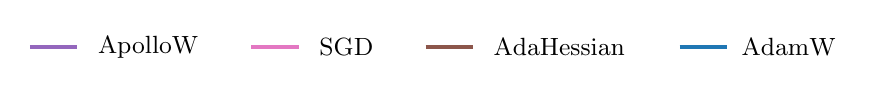
\begin{tikzpicture}[scale=0.75] % Nested TikZ environment
        \small 
        % AdaBelief
 \draw[mediumpurple148103189,  ultra thick] (0,0) -- ++(0.8,0);
 \node[anchor=west] at (1,0) {{ApolloW}}; % Increased spacing
 
 % Adam

 \draw[orchid227119194,  ultra thick] (3.75,0) -- ++(0.8,0);
 \node[anchor=west] at (4.75,0) {{SGD}}; % Increased spacing
 
 % AdaHessian
 \draw[sienna1408675,  ultra thick] (6.7,0) -- ++(0.8,0);
 \node[anchor=west] at (7.7,0) {{AdaHessian}}; % Increased spacing
 
 % Apollo
 \draw[steelblue31119180,  ultra thick] (11,0) -- ++(0.8,0);
 \node[anchor=west] at (11.9,0) {{AdamW}}; % Increased spacing
    
\end{tikzpicture}
};
\end{tikzpicture}
 \\ % Replace with the correct path to your .tex file
    \end{tabular}
    \caption{Evaluation of optimizers on CIFAR-10 using ResNet-110 with the \emph{cosine annealing} learning rate scheduler, where hyperparameters
    are choosen optimally across all optimizers. For better visualization we applied a polynomial transformation, with $\hat{x}=x^\alpha$ and $\alpha=5$, for every $x \in \mathcal{D}$ in the output data $ \mathcal{D}$. }
    \label{fig:cifar-10-cosine-second}
\end{figure}
Using the cosine annealing learning rate scheduler in our first evaluation strategy,
we observe the same ordering of optimizers in terms of generalization and convergence behavior (see Figure~\ref{fig:cifar-10-cosine-real}).
To expand on our second evaluation strategy, Figure \ref{fig:cifar-10-cosine-second}
illustrates the performance of each optimizer when given its optimal set of hyperparameters,
as specified in \cite{apollo}. As previously mentioned, \emph{AdaHessian}, \emph{Apollo} and 
\emph{ApolloW} demonstrate superior performance in terms of generalization error. While both \emph{Apollo} and \emph{ApolloW} are able to converge faster than \emph{AdaHessian},
especially in the early epochs, \emph{ApolloW} converges more slowly than its decoupled first-order counterparts,
\emph{AdamW} and \emph{AdaBelief}.
While \emph{AdaHessian}, \emph{Apollo} and \emph{ApolloW} perform similiar in the setting of 
\ref{fig:cifar-10-cosine-second}, \emph{AdaHessian} exhorts much higher variability when compared to 
\ref{fig:cifar-10-cosine-real}. This observation lends credence to the claim in \cite{apollo} that \emph{Apollo} and \emph{ApolloW} 
may be more practical than \emph{AdaHessian} for real-world applications.\\
Expanding on \emph{Apollo's} better generalization abilities, figure \ref{fig:cifar-10-cosine-second} shows that \emph{Apollo} and \emph{ApolloW} continue to decrease their
test loss even at epoch 164, while \emph{Adam} and \emph{AdamW},
experience a steadily increasing test loss.

In Table \ref{tab:optimizer_comparison_perf}, we can observe the maximum memory consumption
of each optimizer and the duration of one optimization step realtive to \emph{SGD}.
Not surprisingly, \emph{Apollo} and \emph{AdaHessian} both take longer for each step and
consume more memory (see Table \ref{tab:optimizer_comparison_perf}). While the increase in computation time and GPU memory is
rather modest for \emph{Apollo}, we can see that \emph{AdaHessian} takes significantly
longer for computation compared to both \emph{Apollo} and the first-order
 methods, as well as consumes much more memory. This is likely the result of
the second backward pass \emph{AdaHessian} uses to compute the second-order gradients,
which also limits the use of \emph{AdaHessian} in practice.


\begin{table}[h!]
    \centering
    \caption{Accuracy (\%) of different optimizers across CIFAR-10 and TinyImageNet, evaluated on 3 runs (CIFAR-10)}
    \label{tab:optimizer_comparison_acc}
    \begin{tabular}{lcccccccccccc}
        \toprule
        & \multicolumn{2}{c}{CIFAR-10} & \multicolumn{2}{c}{Tiny ImageNet} \\
        \cmidrule(lr){2-3} \cmidrule(lr){4-5}  \cmidrule(lr){6-7} 
        & \textbf{Milestone} & \textbf{Cosine}  & \textbf{Milestone} & \textbf{Cosine}    \\
        \midrule
        SGD         & 87.2 ± 0.86  & 88.17 ± 0.3 & 39.32  & 38.56  \\
        Adam        & 90.8 ± 0.39   & 90.32 ± 0.08  & 43.06 & 43.44    \\
        AdamW       & 90.35 ± 0.06  & 89.99 ± 0.26 & 42  & 41.71 \\
        AdaBelief   & 90.23 ± 0.18  & 90.08 ± 0.18 & 41.88 & 41.72 \\
        RMSProp     & 90.1 ± 0.12   & 89.5 ± 0.33  & 39.4 & 39.9\\
        Apollo      & 91.88 ± 0.38 & \textbf{92.18} ± 0.18  & \textbf{44.96}  & \textbf{44.32}    \\
        ApolloW     & \textbf{92.03} ± 0.08 & 92.02 ± 0.17  & 43.06  & 43.96  \\
        AdaHessian  & 91.64 ± 0.26    &  91.81 ± 0.55 &  44.28& 44.08  \\
        \bottomrule
    \end{tabular}
\end{table}

\begin{table}[h!]
    \centering
    \caption{Time (epochs) until convergence (see \ref{alg:convergence}) of the training loss across CIFAR-10 and TinyImageNet}
    \label{tab:optimizer_comparison_ttc}
    \begin{tabular}{lcccccccccccc}
        \toprule
        & \multicolumn{2}{c}{CIFAR-10} & \multicolumn{2}{c}{Tiny ImageNet} \\
        \cmidrule(lr){2-3} \cmidrule(lr){4-5}  \cmidrule(lr){6-7} 
        & \textbf{Milestone} & \textbf{Cosine}  & \textbf{Milestone} & \textbf{Cosine}    \\
        \midrule
        SGD         & 86 ± 5.0 & 113 ± 1.0 & 44 & \textbf{52} \\
        Adam        & 94 ± 1.0 & 132 ± 1.0& 57 & 84  \\
        AdamW       & 81 ± 0.0 & 112 ± 3.0& \textbf{40} & 59 \\
        AdaBelief   & 81 ± 0.0  &  \textbf{108} ± 4.0& \textbf{40} & 60 \\
        RMSProp     & \textbf{80} ± 0.0  & \textbf{108} ± 1.0& \textbf{40} & 58\\
        Apollo      & 84 ± 1.0 & 125 ± 1.0& 42 & 60   \\
        ApolloW     & 87 ± 1.0 & 137 ± 1.0& 43 & 60  \\
        AdaHessian  & 88 ± 0.0 & 121 ± 2.0& 53 & 72 \\
        \bottomrule
    \end{tabular}
\end{table}
\subsection{Tiny ImageNet}
For the second image classification dataset, we use Tiny ImageNet \cite{tiny_imagenet}.
Tiny ImageNet is a more manageable subset of the well-known ImageNet dataset.
It consists of 100,000 RGB images, each sized 64x64 pixels, across 200 different classes.
For training, we again follow the configuration outlined by \emph{Apollo} \cite{apollo} and utilize a ResNet-18 model with approximately 11.7 million parameters. 
We found that deeper ResNet architectures, like \emph{ResNet-50}, lead to significantly more overfitting during training.
The training is conducted with a batch size of 256. We implement milestone decay, adjusting the 
learning rate at epochs 40 and 80 by a factor of $\gamma=0.1$.
The model is trained for 120 epochs, employing both milestone decay and cosine annealing strategies. Our strategy for hyperparameter evaluation remains consistent with those used for CIFAR-10. We first 
test the optimizers' performance by evaluating the second-order optimizers on the optimal values of 
the popular first-order optimizers. These settings are given in \ref{tab:tiny-real-comp}

\begin{figure}[h!]
    \centering
    \begin{tabular}{cc}
        % This file was created with tikzplotlib v0.10.1.
\begin{tikzpicture}[scale=0.75]

    \definecolor{crimson2143940}{RGB}{214,39,40}
    \definecolor{darkgrey176}{RGB}{176,176,176}
    \definecolor{darkorange25512714}{RGB}{255,127,14}
    \definecolor{forestgreen4416044}{RGB}{44,160,44}
    \definecolor{grey127}{RGB}{127,127,127}
    \definecolor{lightgrey204}{RGB}{204,204,204}
    \definecolor{mediumpurple148103189}{RGB}{148,103,189}
    \definecolor{orchid227119194}{RGB}{227,119,194}
    \definecolor{sienna1408675}{RGB}{140,86,75}
    \definecolor{steelblue31119180}{RGB}{31,119,180}
    
    \begin{groupplot}[group style={group size=2 by 2,
        horizontal sep=1cm,  % Adjust horizontal spacing
        vertical sep=2cm}]
    \nextgroupplot[
    tick align=outside,
    tick pos=left,
    title={Training Accuracy (milestone)},
    x grid style={darkgrey176},
    xlabel={Epochs},
    xmin=-5.95, xmax=124.95,
    xtick style={color=black},
    y grid style={darkgrey176},
    ymin=-0.0438179347826087, ymax=1.04809382992327,
    ytick style={color=black}
    ]
    \addplot [semithick, steelblue31119180]
    table {%
    0 0.0869964833759591
    1 0.182384910485933
    2 0.243795955882353
    3 0.290970668158568
    4 0.328944213554987
    5 0.366388267263427
    6 0.400115888746803
    7 0.431116128516624
    8 0.461437020460358
    9 0.492237452046036
    10 0.520230578644501
    11 0.551980099104859
    12 0.582340952685422
    13 0.61475983056266
    14 0.649236732736573
    15 0.678978180946292
    16 0.710398017902813
    17 0.741018622122762
    18 0.765055546675192
    19 0.786195252557545
    20 0.809363011508951
    21 0.82717591112532
    22 0.838604939258312
    23 0.853140984654731
    24 0.864350223785166
    25 0.871343510230179
    26 0.880654571611253
    27 0.88960597826087
    28 0.891264386189258
    29 0.898867087595908
    30 0.90174432544757
    31 0.909426950127877
    32 0.912124360613811
    33 0.915640984654731
    34 0.916979699488491
    35 0.921315537084399
    36 0.923023897058823
    37 0.929138027493606
    38 0.929817375319693
    39 0.930137068414322
    40 0.965353260869565
    41 0.977411684782609
    42 0.981297953964194
    43 0.984355019181586
    44 0.985703724424552
    45 0.988341192455243
    46 0.988750799232737
    47 0.990309303069054
    48 0.990579044117647
    49 0.991458200127877
    50 0.992087595907928
    51 0.992147538363171
    52 0.992617087595908
    53 0.992677030051151
    54 0.992886828644501
    55 0.993436301150895
    56 0.994015744884911
    57 0.993965792838875
    58 0.994215553069054
    59 0.994285485933504
    60 0.995104699488491
    61 0.994904891304348
    62 0.99528452685422
    63 0.99556425831202
    64 0.995204603580563
    65 0.995704124040921
    66 0.995804028132992
    67 0.995804028132992
    68 0.99556425831202
    69 0.996193654092072
    70 0.9959538842711
    71 0.996253596547315
    72 0.995993845907928
    73 0.996283567774936
    74 0.996183663682864
    75 0.995963874680307
    76 0.996413443094629
    77 0.996223625319693
    78 0.996423433503836
    79 0.996413443094629
    80 0.997082800511509
    81 0.997182704603581
    82 0.997192695012788
    83 0.997272618286445
    84 0.997592311381074
    85 0.997812100383632
    86 0.997592311381074
    87 0.997722186700767
    88 0.997622282608696
    89 0.99778212915601
    90 0.998001918158568
    91 0.997632273017903
    92 0.997991927749361
    93 0.997822090792839
    94 0.997872042838875
    95 0.997722186700767
    96 0.997832081202046
    97 0.997931985294118
    98 0.998041879795396
    99 0.998101822250639
    100 0.997971946930946
    101 0.997991927749361
    102 0.998141783887468
    103 0.998041879795396
    104 0.997872042838875
    105 0.998101822250639
    106 0.998191735933504
    107 0.997772138746803
    108 0.998141783887468
    109 0.998431505754476
    110 0.997892023657289
    111 0.998171755115089
    112 0.998061860613811
    113 0.998281649616368
    114 0.998361572890026
    115 0.998141783887468
    116 0.997961956521739
    117 0.998101822250639
    118 0.998181745524297
    119 0.99845148657289
    };
    \addplot [semithick, darkorange25512714]
    table {%
    0 0.0859874520460358
    1 0.178768382352941
    2 0.233046275575448
    3 0.273677269820972
    4 0.306056186061381
    5 0.337006473785166
    6 0.361433024296675
    7 0.385669757033248
    8 0.40719908887468
    9 0.426330722506394
    10 0.442994725063939
    11 0.459958439897698
    12 0.4727961157289
    13 0.490199408567775
    14 0.504255914322251
    15 0.515615009590793
    16 0.530191016624041
    17 0.538503037084399
    18 0.552169916879795
    19 0.560152253836317
    20 0.571711157289003
    21 0.582121163682864
    22 0.591901774296675
    23 0.603190936700767
    24 0.610473945012788
    25 0.617866847826087
    26 0.625299712276215
    27 0.633062260230179
    28 0.64055506713555
    29 0.645909926470588
    30 0.654022138746803
    31 0.657688618925831
    32 0.662024456521739
    33 0.670156649616368
    34 0.674982017263427
    35 0.678089034526854
    36 0.684303069053708
    37 0.690626998081841
    38 0.693714034526854
    39 0.696671195652174
    40 0.804217950767263
    41 0.839853740409207
    42 0.857846467391304
    43 0.868696051790281
    44 0.876938139386189
    45 0.885489929667519
    46 0.893462276214834
    47 0.898827125959079
    48 0.904861333120205
    49 0.907678628516624
    50 0.913063459079284
    51 0.915970668158568
    52 0.920686141304348
    53 0.922634271099744
    54 0.925491528132992
    55 0.929667519181586
    56 0.930716512148338
    57 0.934273097826087
    58 0.935412004475703
    59 0.937939578005115
    60 0.939538043478261
    61 0.941725943094629
    62 0.942275415601023
    63 0.945322490409207
    64 0.946511349104859
    65 0.947280610613811
    66 0.948889066496164
    67 0.951136908567775
    68 0.952545556265985
    69 0.951936141304348
    70 0.955023177749361
    71 0.954803388746803
    72 0.955822410485934
    73 0.956202046035806
    74 0.95777054028133
    75 0.959199168797954
    76 0.959648737212276
    77 0.960517902813299
    78 0.960847586317136
    79 0.960967471227621
    80 0.966662004475703
    81 0.969709079283887
    82 0.970518302429668
    83 0.972506393861893
    84 0.972945971867008
    85 0.972636269181586
    86 0.972596307544757
    87 0.97480418797954
    88 0.974124840153453
    89 0.974534446930946
    90 0.974654331841432
    91 0.976262787723785
    92 0.975763267263427
    93 0.975873161764706
    94 0.976742327365729
    95 0.976872202685422
    96 0.976612452046036
    97 0.97790121483376
    98 0.976372682225064
    99 0.976812260230179
    100 0.97804108056266
    101 0.977351742327366
    102 0.978390744884911
    103 0.977741368286445
    104 0.977561540920716
    105 0.978930226982097
    106 0.978520620204604
    107 0.978170955882353
    108 0.979010150255754
    109 0.978730418797954
    110 0.978620524296675
    111 0.978590553069054
    112 0.978600543478261
    113 0.979469709079284
    114 0.98039881713555
    115 0.980638586956522
    116 0.980488730818414
    117 0.980498721227621
    118 0.980039162404092
    119 0.980548673273657
    };
    \addplot [semithick, forestgreen4416044]
    table {%
    0 0.0859574808184143
    1 0.180526694373402
    2 0.238700847186701
    3 0.28649496483376
    4 0.325087915601023
    5 0.359275095907928
    6 0.393142583120205
    7 0.425511508951407
    8 0.456931345907928
    9 0.486512947570332
    10 0.518232496803069
    11 0.548863091432225
    12 0.582710597826087
    13 0.615159446930946
    14 0.647248641304348
    15 0.683124200767263
    16 0.711447010869565
    17 0.741248401534527
    18 0.763157368925831
    19 0.794417359335038
    20 0.808493845907928
    21 0.826476582480818
    22 0.843520220588235
    23 0.851662404092072
    24 0.864460118286445
    25 0.87285206202046
    26 0.882512787723785
    27 0.884930466751918
    28 0.892043638107417
    29 0.898057864450128
    30 0.904551630434783
    31 0.90955682544757
    32 0.912613890664962
    33 0.915411205242967
    34 0.917509191176471
    35 0.922134750639386
    36 0.922054827365729
    37 0.928188938618926
    38 0.930486732736573
    39 0.931575687340154
    40 0.965802829283887
    41 0.976382672634271
    42 0.981687579923274
    43 0.984025335677749
    44 0.986093350383632
    45 0.988121403452685
    46 0.988730818414322
    47 0.989570012787724
    48 0.990029571611253
    49 0.991608056265985
    50 0.991548113810742
    51 0.992007672634271
    52 0.992956761508951
    53 0.992527173913043
    54 0.993316416240409
    55 0.993496243606138
    56 0.993436301150895
    57 0.994365409207161
    58 0.994365409207161
    59 0.994565217391304
    60 0.995114689897698
    61 0.994675111892583
    62 0.995154651534527
    63 0.995184622762148
    64 0.995264546035806
    65 0.995374440537084
    66 0.995574248721228
    67 0.995754076086957
    68 0.995724104859335
    69 0.995903932225064
    70 0.995863970588235
    71 0.996073769181586
    72 0.996073769181586
    73 0.996073769181586
    74 0.9962336157289
    75 0.996153692455243
    76 0.996353500639386
    77 0.996843030690537
    78 0.996513347186701
    79 0.996333519820972
    80 0.997142742966752
    81 0.997182704603581
    82 0.997632273017903
    83 0.997182704603581
    84 0.99743246483376
    85 0.997412484015345
    86 0.997632273017903
    87 0.997772138746803
    88 0.997552349744246
    89 0.997492407289003
    90 0.997921994884911
    91 0.997662244245524
    92 0.997792119565217
    93 0.998131793478261
    94 0.997772138746803
    95 0.997832081202046
    96 0.997961956521739
    97 0.997892023657289
    98 0.998191735933504
    99 0.997912004475703
    100 0.998051870204604
    101 0.998161764705882
    102 0.998061860613811
    103 0.998131793478261
    104 0.998091831841432
    105 0.998131793478261
    106 0.998321611253197
    107 0.998231697570332
    108 0.998231697570332
    109 0.998131793478261
    110 0.998131793478261
    111 0.998141783887468
    112 0.998081841432225
    113 0.997912004475703
    114 0.998261668797954
    115 0.998461476982097
    116 0.998431505754476
    117 0.998231697570332
    118 0.998321611253197
    119 0.998181745524297
    };
    \addplot [semithick, crimson2143940]
    table {%
    0 0.0712515984654731
    1 0.16170476342711
    2 0.217381313938619
    3 0.259400975063939
    4 0.291440217391304
    5 0.322550351662404
    6 0.34691695971867
    7 0.372822090792839
    8 0.397678228900256
    9 0.421335517902813
    10 0.44119645140665
    11 0.462116368286445
    12 0.484135230179028
    13 0.505214993606138
    14 0.525745284526854
    15 0.550081921355499
    16 0.567625079923274
    17 0.589144421355499
    18 0.612931585677749
    19 0.632063219309463
    20 0.654012148337596
    21 0.672834079283887
    22 0.695582241048593
    23 0.714454124040921
    24 0.732696611253197
    25 0.7541859814578
    26 0.769781010230179
    27 0.782678628516624
    28 0.80138067455243
    29 0.815686940537084
    30 0.829553628516624
    31 0.837675831202046
    32 0.854020140664962
    33 0.861143302429668
    34 0.869794996803069
    35 0.880125079923274
    36 0.88752797314578
    37 0.89607976342711
    38 0.900495524296675
    39 0.909426950127877
    40 0.952605498721228
    41 0.968440297314578
    42 0.973615329283887
    43 0.976142902813299
    44 0.979889306265985
    45 0.980298913043478
    46 0.98282648657289
    47 0.983545796035806
    48 0.984794597186701
    49 0.985933503836317
    50 0.985953484654731
    51 0.987232257033248
    52 0.987871643222506
    53 0.98775175831202
    54 0.988291240409207
    55 0.988710837595908
    56 0.990269341432225
    57 0.989929667519182
    58 0.989819773017903
    59 0.990609015345269
    60 0.990808823529412
    61 0.991298353580563
    62 0.991068574168798
    63 0.991608056265985
    64 0.992227461636829
    65 0.992167519181586
    66 0.9924672314578
    67 0.992687020460358
    68 0.992846867007673
    69 0.992647058823529
    70 0.993416320332481
    71 0.992906809462916
    72 0.993336397058823
    73 0.99352621483376
    74 0.993686061381074
    75 0.993326406649616
    76 0.994455322890026
    77 0.994175591432225
    78 0.994415361253197
    79 0.994285485933504
    80 0.994495284526854
    81 0.994455322890026
    82 0.994675111892583
    83 0.995114689897698
    84 0.994695092710997
    85 0.994535246163683
    86 0.994834958439898
    87 0.995164641943734
    88 0.99461516943734
    89 0.994824968030691
    90 0.99535445971867
    91 0.99514466112532
    92 0.994984814578005
    93 0.994844948849105
    94 0.994884910485934
    95 0.99528452685422
    96 0.994994804987212
    97 0.99521459398977
    98 0.99507472826087
    99 0.995414402173913
    100 0.994874920076726
    101 0.99549432544757
    102 0.995054747442455
    103 0.995204603580563
    104 0.995184622762148
    105 0.995174632352941
    106 0.995204603580563
    107 0.995064737851662
    108 0.995094709079284
    109 0.995184622762148
    110 0.995374440537084
    111 0.995973865089514
    112 0.995654171994885
    113 0.995044757033248
    114 0.995604219948849
    115 0.995484335038363
    116 0.995444373401535
    117 0.99556425831202
    118 0.995194613171355
    119 0.995374440537084
    };
    \addplot [semithick, mediumpurple148103189]
    table {%
    0 0.0714813778772379
    1 0.165461157289003
    2 0.220168638107417
    3 0.260829603580563
    4 0.295676150895141
    5 0.32442854859335
    6 0.352211876598465
    7 0.376958120204604
    8 0.402523577365729
    9 0.425321691176471
    10 0.447959958439898
    11 0.470098705242967
    12 0.492217471227621
    13 0.516763906649616
    14 0.539671914961637
    15 0.561600863171355
    16 0.585637787723785
    17 0.60708719629156
    18 0.631253996163683
    19 0.656240009590793
    20 0.675831202046036
    21 0.698449488491049
    22 0.720418398337596
    23 0.737162324168798
    24 0.756573689258312
    25 0.780380834398977
    26 0.799242726982097
    27 0.815107496803069
    28 0.828764386189258
    29 0.843400335677749
    30 0.855918318414322
    31 0.869345428388747
    32 0.877837276214834
    33 0.885779651534527
    34 0.895030770460358
    35 0.902853260869565
    36 0.911854619565217
    37 0.917139546035806
    38 0.922744165601023
    39 0.928089034526854
    40 0.961267183503836
    41 0.972496403452685
    42 0.97589314258312
    43 0.978290840792839
    44 0.980948289641944
    45 0.98148777173913
    46 0.983725623401535
    47 0.984624760230179
    48 0.984744645140665
    49 0.986043398337596
    50 0.986423033887468
    51 0.986952525575448
    52 0.987322170716113
    53 0.987492007672634
    54 0.988610933503836
    55 0.988710837595908
    56 0.98895060741688
    57 0.989629955242967
    58 0.98961996483376
    59 0.99077885230179
    60 0.991068574168798
    61 0.991388267263427
    62 0.991298353580563
    63 0.991388267263427
    64 0.99123841112532
    65 0.991877797314578
    66 0.992077605498721
    67 0.991987691815857
    68 0.992077605498721
    69 0.992826886189258
    70 0.992377317774936
    71 0.992477221867008
    72 0.993076646419437
    73 0.992607097186701
    74 0.993476262787724
    75 0.99366608056266
    76 0.993116608056266
    77 0.99366608056266
    78 0.993845907928389
    79 0.994225543478261
    80 0.99387587915601
    81 0.993925831202046
    82 0.99387587915601
    83 0.994775015984655
    84 0.994395380434783
    85 0.994385390025575
    86 0.994215553069054
    87 0.994525255754476
    88 0.994435342071611
    89 0.994365409207161
    90 0.993755994245524
    91 0.994435342071611
    92 0.994045716112532
    93 0.994894900895141
    94 0.99440537084399
    95 0.994315457161125
    96 0.994375399616368
    97 0.994275495524297
    98 0.994315457161125
    99 0.994525255754476
    100 0.995004795396419
    101 0.994345428388747
    102 0.994655131074169
    103 0.994355418797954
    104 0.994465313299233
    105 0.994365409207161
    106 0.994345428388747
    107 0.994884910485934
    108 0.994565217391304
    109 0.994655131074169
    110 0.994315457161125
    111 0.99468510230179
    112 0.994695092710997
    113 0.995114689897698
    114 0.995024776214834
    115 0.994964833759591
    116 0.994425351662404
    117 0.994804987212276
    118 0.995014785805627
    119 0.994745044757033
    };
    \addplot [semithick, sienna1408675]
    table {%
    0 0.00901134910485933
    1 0.0212296195652174
    2 0.0364749840153453
    3 0.0505714514066496
    4 0.0653972186700767
    5 0.0770760070332481
    6 0.0892643062659847
    7 0.10068334398977
    8 0.112641863810742
    9 0.123821131713555
    10 0.133361972506394
    11 0.142872842071611
    12 0.150255754475703
    13 0.1600163842711
    14 0.168558184143223
    15 0.175271739130435
    16 0.184353021099744
    17 0.191086556905371
    18 0.1990788842711
    19 0.202895220588235
    20 0.210697730179028
    21 0.217970748081841
    22 0.222236652813299
    23 0.226302749360614
    24 0.234774616368286
    25 0.239360214194373
    26 0.242387308184143
    27 0.24778212915601
    28 0.252907209079284
    29 0.257782528772379
    30 0.260749680306905
    31 0.266624040920716
    32 0.270360453964194
    33 0.273387547953964
    34 0.277893222506394
    35 0.281499760230179
    36 0.285326086956522
    37 0.291110533887468
    38 0.294687100383632
    39 0.298033887468031
    40 0.304407768542199
    41 0.306885390025575
    42 0.305846387468031
    43 0.307145140664962
    44 0.30778452685422
    45 0.30764466112532
    46 0.307494804987212
    47 0.30880354859335
    48 0.308443893861893
    49 0.310961476982097
    50 0.309912484015345
    51 0.312549952046036
    52 0.312949568414322
    53 0.311460997442455
    54 0.311081361892583
    55 0.313199328644501
    56 0.312300191815857
    57 0.314837755754476
    58 0.314408168158568
    59 0.313628916240409
    60 0.314847746163683
    61 0.315147458439898
    62 0.314208359974425
    63 0.316685981457801
    64 0.316176470588235
    65 0.31573689258312
    66 0.31661604859335
    67 0.317085597826087
    68 0.319103660485934
    69 0.316845828005115
    70 0.319223545396419
    71 0.317175511508951
    72 0.319543238491049
    73 0.320352461636829
    74 0.321271579283887
    75 0.320812020460358
    76 0.319543238491049
    77 0.321771099744246
    78 0.32105179028133
    79 0.322700207800512
    80 0.323369565217391
    81 0.32193094629156
    82 0.322949968030691
    83 0.322050831202046
    84 0.322590313299233
    85 0.323009910485934
    86 0.32400895140665
    87 0.32414881713555
    88 0.325447570332481
    89 0.323189737851662
    90 0.323729219948849
    91 0.322750159846547
    92 0.322710198209719
    93 0.32354939258312
    94 0.323169757033248
    95 0.325437579923274
    96 0.323649296675192
    97 0.323829124040921
    98 0.324068893861893
    99 0.324198769181586
    100 0.324388586956522
    101 0.324498481457801
    102 0.32319972826087
    103 0.323929028132992
    104 0.323699248721228
    105 0.324058903452685
    106 0.324548433503836
    107 0.323179747442455
    108 0.3243586157289
    109 0.324038922634271
    110 0.323739210358056
    111 0.325677349744246
    112 0.323029891304348
    113 0.326046994884911
    114 0.324828164961637
    115 0.324928069053708
    116 0.325587436061381
    117 0.323829124040921
    118 0.325747282608696
    119 0.324228740409207
    };
    \addplot [semithick, orchid227119194]
    table {%
    0 0.00581441815856778
    1 0.00906130115089514
    2 0.0132472826086957
    3 0.0204703484654731
    4 0.0248960997442455
    5 0.0303708439897698
    6 0.0354259910485933
    7 0.0404611572890026
    8 0.0440976662404092
    9 0.0491927749360614
    10 0.0532688618925831
    11 0.0586037404092072
    12 0.0617607097186701
    13 0.0669357416879795
    14 0.0707320971867008
    15 0.0732197090792839
    16 0.0767263427109974
    17 0.080232976342711
    18 0.0856078164961637
    19 0.0885350063938619
    20 0.0920216592071611
    21 0.0948489450127877
    22 0.0998441496163683
    23 0.103130994245524
    24 0.107067215473146
    25 0.109464913682864
    26 0.112821691176471
    27 0.116807864450128
    28 0.120814018542199
    29 0.125409606777494
    30 0.127547554347826
    31 0.131383871483376
    32 0.134321051790281
    33 0.140075527493606
    34 0.140824808184143
    35 0.144511269181586
    36 0.147378516624041
    37 0.151374680306905
    38 0.154471707161125
    39 0.156559702685422
    40 0.159456921355499
    41 0.159476902173913
    42 0.161534926470588
    43 0.160445971867008
    44 0.159936460997442
    45 0.160326086956522
    46 0.160925511508951
    47 0.160885549872123
    48 0.161464993606138
    49 0.162364130434783
    50 0.162154331841432
    51 0.162084398976982
    52 0.16466192455243
    53 0.163812739769821
    54 0.163003516624041
    55 0.164831761508951
    56 0.163582960358056
    57 0.165601023017903
    58 0.165930706521739
    59 0.166240409207161
    60 0.166260390025575
    61 0.167309382992327
    62 0.167059622762148
    63 0.166929747442455
    64 0.166610054347826
    65 0.164991608056266
    66 0.167349344629156
    67 0.167259430946292
    68 0.167289402173913
    69 0.166370284526854
    70 0.169337436061381
    71 0.169507273017903
    72 0.168208519820972
    73 0.169167599104859
    74 0.169097666240409
    75 0.169067695012788
    76 0.169836956521739
    77 0.17039641943734
    78 0.171924952046036
    79 0.171215632992327
    80 0.170166640025575
    81 0.171914961636829
    82 0.170516304347826
    83 0.170496323529412
    84 0.171625239769821
    85 0.170826007033248
    86 0.169257512787724
    87 0.171035805626598
    88 0.171195652173913
    89 0.171365489130435
    90 0.17092591112532
    91 0.172854060102302
    92 0.171645220588235
    93 0.170875959079284
    94 0.170656170076726
    95 0.171465393222506
    96 0.170456361892583
    97 0.172164721867008
    98 0.171865009590793
    99 0.172414482097187
    100 0.171195652173913
    101 0.171875
    102 0.17275415601023
    103 0.171255594629156
    104 0.171924952046036
    105 0.172074808184143
    106 0.171375479539642
    107 0.170726102941176
    108 0.171445412404092
    109 0.170945891943734
    110 0.170136668797954
    111 0.171795076726343
    112 0.172554347826087
    113 0.171425431585678
    114 0.172514386189258
    115 0.172324568414322
    116 0.172394501278772
    117 0.172254635549872
    118 0.172044836956522
    119 0.171685182225064
    };
    \addplot [semithick, grey127]
    table {%
    0 0.0522498401534527
    1 0.155280930306905
    2 0.217930786445013
    3 0.264585997442455
    4 0.303938219309463
    5 0.338774776214834
    6 0.371523337595908
    7 0.400465553069054
    8 0.430246962915601
    9 0.456941336317136
    10 0.488780770460358
    11 0.517992726982097
    12 0.548992966751918
    13 0.579403772378517
    14 0.609994405370844
    15 0.640674952046036
    16 0.671315537084399
    17 0.699718270460358
    18 0.727181905370844
    19 0.752437659846547
    20 0.775915121483376
    21 0.795436381074169
    22 0.811281170076726
    23 0.826446611253197
    24 0.841821851023018
    25 0.850503516624041
    26 0.860963475063939
    27 0.870774056905371
    28 0.877397698209719
    29 0.886009430946292
    30 0.89136429028133
    31 0.896609255115089
    32 0.902193893861893
    33 0.906160086317136
    34 0.910915521099744
    35 0.914192375319693
    36 0.917059622762148
    37 0.921195652173913
    38 0.923683264066496
    39 0.927109974424552
    40 0.961177269820972
    41 0.976292758951407
    42 0.981597666240409
    43 0.98416520140665
    44 0.985374040920716
    45 0.987252237851662
    46 0.988521019820972
    47 0.989410166240409
    48 0.990309303069054
    49 0.990698929028133
    50 0.991468190537084
    51 0.991887787723785
    52 0.992537164322251
    53 0.993236492966752
    54 0.993076646419437
    55 0.993186540920716
    56 0.993845907928389
    57 0.994325447570332
    58 0.994295476342711
    59 0.994325447570332
    60 0.994894900895141
    61 0.99528452685422
    62 0.994854939258312
    63 0.995104699488491
    64 0.995524296675192
    65 0.995524296675192
    66 0.995364450127877
    67 0.995574248721228
    68 0.99588395140665
    69 0.995204603580563
    70 0.996283567774936
    71 0.995993845907928
    72 0.996213634910486
    73 0.996483375959079
    74 0.99616368286445
    75 0.996533328005115
    76 0.996473385549872
    77 0.996773097826087
    78 0.996313539002558
    79 0.996453404731458
    80 0.997012867647059
    81 0.997142742966752
    82 0.997182704603581
    83 0.997282608695652
    84 0.99757233056266
    85 0.997792119565217
    86 0.997762148337596
    87 0.997892023657289
    88 0.997512388107417
    89 0.998011908567775
    90 0.997971946930946
    91 0.99764226342711
    92 0.997862052429668
    93 0.997862052429668
    94 0.997961956521739
    95 0.99757233056266
    96 0.997762148337596
    97 0.997862052429668
    98 0.997902014066496
    99 0.99785206202046
    100 0.997822090792839
    101 0.99785206202046
    102 0.998251678388747
    103 0.997941975703325
    104 0.997862052429668
    105 0.998031889386189
    106 0.99824168797954
    107 0.998041879795396
    108 0.998131793478261
    109 0.998201726342711
    110 0.998341592071611
    111 0.998121803069054
    112 0.998221707161125
    113 0.997941975703325
    114 0.998431505754476
    115 0.998261668797954
    116 0.998271659207161
    117 0.998331601662404
    118 0.998051870204604
    119 0.998291640025575
    };
    
    \nextgroupplot[
    tick align=outside,
    tick pos=left,
    title={Test Accuracy (milestone)},
    x grid style={darkgrey176},
    xlabel={Epochs},
    xmin=-5.95, xmax=124.95,
    xtick style={color=black},
    y grid style={darkgrey176},
    ymin=-0.0144481803797468, ymax=0.473111155063291,
    ytick style={color=black}
    ]
    \addplot [semithick, steelblue31119180]
    table {%
    0 0.153777689873418
    1 0.23407832278481
    2 0.255241297468354
    3 0.309928797468354
    4 0.320411392405063
    5 0.340189873417722
    6 0.365308544303797
    7 0.379845727848101
    8 0.400909810126582
    9 0.388152689873418
    10 0.404667721518987
    11 0.403975474683544
    12 0.40535996835443
    13 0.412282436708861
    14 0.407733386075949
    15 0.398931962025316
    16 0.409414556962025
    17 0.397943037974684
    18 0.398239715189873
    19 0.389339398734177
    20 0.38251582278481
    21 0.39092167721519
    22 0.386867088607595
    23 0.392108386075949
    24 0.390723892405063
    25 0.387460443037975
    26 0.382713607594937
    27 0.388251582278481
    28 0.390229430379747
    29 0.393097310126582
    30 0.387361550632911
    31 0.381823575949367
    32 0.384790348101266
    33 0.391910601265823
    34 0.379746835443038
    35 0.378362341772152
    36 0.388350474683544
    37 0.386372626582278
    38 0.380834651898734
    39 0.385878164556962
    40 0.40625
    41 0.413073575949367
    42 0.414458069620253
    43 0.4140625
    44 0.413666930379747
    45 0.414853639240506
    46 0.413271360759494
    47 0.41346914556962
    48 0.415051424050633
    49 0.41317246835443
    50 0.414754746835443
    51 0.419106012658228
    52 0.418215981012658
    53 0.418018196202532
    54 0.41495253164557
    55 0.414458069620253
    56 0.420094936708861
    57 0.418908227848101
    58 0.415446993670886
    59 0.415842563291139
    60 0.415249208860759
    61 0.416139240506329
    62 0.418908227848101
    63 0.41465585443038
    64 0.415743670886076
    65 0.420292721518987
    66 0.41435917721519
    67 0.414458069620253
    68 0.420292721518987
    69 0.415051424050633
    70 0.418413765822785
    71 0.415941455696203
    72 0.413568037974684
    73 0.416139240506329
    74 0.418611550632911
    75 0.421677215189873
    76 0.416139240506329
    77 0.415941455696203
    78 0.418710443037975
    79 0.416534810126582
    80 0.418314873417722
    81 0.418314873417722
    82 0.415644778481013
    83 0.418809335443038
    84 0.418314873417722
    85 0.419303797468354
    86 0.418314873417722
    87 0.419204905063291
    88 0.418512658227848
    89 0.421083860759494
    90 0.419402689873418
    91 0.418512658227848
    92 0.417029272151899
    93 0.419204905063291
    94 0.417424841772152
    95 0.422270569620253
    96 0.421479430379747
    97 0.420391613924051
    98 0.420193829113924
    99 0.419501582278481
    100 0.416238132911392
    101 0.417622626582278
    102 0.418117088607595
    103 0.419106012658228
    104 0.419204905063291
    105 0.42128164556962
    106 0.42157832278481
    107 0.421973892405063
    108 0.422270569620253
    109 0.418117088607595
    110 0.416534810126582
    111 0.421776107594937
    112 0.419699367088608
    113 0.42098496835443
    114 0.419798259493671
    115 0.419699367088608
    116 0.422270569620253
    117 0.419303797468354
    118 0.419600474683544
    119 0.421479430379747
    };
    \addplot [semithick, darkorange25512714]
    table {%
    0 0.125197784810127
    1 0.196004746835443
    2 0.232199367088608
    3 0.286590189873418
    4 0.296479430379747
    5 0.326542721518987
    6 0.331487341772152
    7 0.363726265822785
    8 0.368769778481013
    9 0.375098892405063
    10 0.382911392405063
    11 0.395767405063291
    12 0.407832278481013
    13 0.41346914556962
    14 0.413073575949367
    15 0.415545886075949
    16 0.414754746835443
    17 0.405755537974684
    18 0.407238924050633
    19 0.416930379746835
    20 0.431269778481013
    21 0.419798259493671
    22 0.413666930379747
    23 0.416139240506329
    24 0.419897151898734
    25 0.410007911392405
    26 0.413073575949367
    27 0.418018196202532
    28 0.40625
    29 0.404568829113924
    30 0.406744462025316
    31 0.409909018987342
    32 0.41376582278481
    33 0.413568037974684
    34 0.410799050632911
    35 0.417029272151899
    36 0.411491297468354
    37 0.410799050632911
    38 0.41465585443038
    39 0.40535996835443
    40 0.440961234177215
    41 0.450949367088608
    42 0.447389240506329
    43 0.449268196202532
    44 0.447092563291139
    45 0.449564873417722
    46 0.448872626582278
    47 0.447982594936709
    48 0.448674841772152
    49 0.446795886075949
    50 0.44620253164557
    51 0.441950158227848
    52 0.445213607594937
    53 0.441554588607595
    54 0.442840189873418
    55 0.437994462025316
    56 0.44471914556962
    57 0.441060126582278
    58 0.441554588607595
    59 0.441356803797468
    60 0.438686708860759
    61 0.438785601265823
    62 0.441554588607595
    63 0.439675632911392
    64 0.441653481012658
    65 0.439477848101266
    66 0.439972310126582
    67 0.438785601265823
    68 0.439675632911392
    69 0.437005537974684
    70 0.440071202531646
    71 0.438587816455696
    72 0.438884493670886
    73 0.434038765822785
    74 0.438983386075949
    75 0.43690664556962
    76 0.437895569620253
    77 0.433445411392405
    78 0.435818829113924
    79 0.433840981012658
    80 0.435917721518987
    81 0.434236550632911
    82 0.435126582278481
    83 0.435324367088608
    84 0.432060917721519
    85 0.436708860759494
    86 0.435621044303797
    87 0.43660996835443
    88 0.439873417721519
    89 0.433840981012658
    90 0.434533227848101
    91 0.435719936708861
    92 0.438291139240506
    93 0.436016613924051
    94 0.439280063291139
    95 0.4375
    96 0.437401107594937
    97 0.43660996835443
    98 0.439873417721519
    99 0.439873417721519
    100 0.433939873417722
    101 0.436807753164557
    102 0.437598892405063
    103 0.437104430379747
    104 0.437104430379747
    105 0.439181170886076
    106 0.437895569620253
    107 0.440565664556962
    108 0.436313291139241
    109 0.440862341772152
    110 0.440367879746835
    111 0.437104430379747
    112 0.437302215189873
    113 0.440268987341772
    114 0.437005537974684
    115 0.439082278481013
    116 0.439082278481013
    117 0.438686708860759
    118 0.440961234177215
    119 0.440763449367089
    };
    \addplot [semithick, forestgreen4416044]
    table {%
    0 0.143789556962025
    1 0.212519778481013
    2 0.241198575949367
    3 0.300731803797468
    4 0.322784810126582
    5 0.35067246835443
    6 0.355221518987342
    7 0.370450949367089
    8 0.358386075949367
    9 0.401799841772152
    10 0.398536392405063
    11 0.406645569620253
    12 0.399624208860759
    13 0.402294303797468
    14 0.409018987341772
    15 0.396954113924051
    16 0.400019778481013
    17 0.396459651898734
    18 0.393789556962025
    19 0.388943829113924
    20 0.389537183544304
    21 0.389636075949367
    22 0.381428006329114
    23 0.385581487341772
    24 0.380933544303797
    25 0.385779272151899
    26 0.382416930379747
    27 0.376384493670886
    28 0.385779272151899
    29 0.380142405063291
    30 0.380340189873418
    31 0.38221914556962
    32 0.384295886075949
    33 0.38340585443038
    34 0.381131329113924
    35 0.389240506329114
    36 0.382120253164557
    37 0.377768987341772
    38 0.377966772151899
    39 0.387757120253165
    40 0.408623417721519
    41 0.407535601265823
    42 0.412579113924051
    43 0.41435917721519
    44 0.41346914556962
    45 0.410106803797468
    46 0.411095727848101
    47 0.410502373417722
    48 0.412776898734177
    49 0.411985759493671
    50 0.412183544303797
    51 0.413073575949367
    52 0.41495253164557
    53 0.416831487341772
    54 0.413963607594937
    55 0.416337025316456
    56 0.415150316455696
    57 0.41465585443038
    58 0.416040348101266
    59 0.418908227848101
    60 0.412678006329114
    61 0.417227056962025
    62 0.412084651898734
    63 0.416732594936709
    64 0.410304588607595
    65 0.413271360759494
    66 0.413864715189873
    67 0.412282436708861
    68 0.413370253164557
    69 0.41435917721519
    70 0.413073575949367
    71 0.412480221518987
    72 0.414260284810127
    73 0.415842563291139
    74 0.414161392405063
    75 0.417128164556962
    76 0.412776898734177
    77 0.411787974683544
    78 0.4140625
    79 0.412282436708861
    80 0.417325949367089
    81 0.415348101265823
    82 0.418215981012658
    83 0.416633702531646
    84 0.415941455696203
    85 0.41495253164557
    86 0.415644778481013
    87 0.415743670886076
    88 0.415446993670886
    89 0.415150316455696
    90 0.417128164556962
    91 0.417820411392405
    92 0.415446993670886
    93 0.417325949367089
    94 0.417820411392405
    95 0.418018196202532
    96 0.417128164556962
    97 0.418314873417722
    98 0.417128164556962
    99 0.419798259493671
    100 0.416831487341772
    101 0.416633702531646
    102 0.416139240506329
    103 0.419106012658228
    104 0.419402689873418
    105 0.418710443037975
    106 0.419501582278481
    107 0.416238132911392
    108 0.419699367088608
    109 0.419007120253165
    110 0.420787183544304
    111 0.418611550632911
    112 0.417721518987342
    113 0.420391613924051
    114 0.418413765822785
    115 0.417721518987342
    116 0.416831487341772
    117 0.418018196202532
    118 0.415743670886076
    119 0.416534810126582
    };
    \addplot [semithick, crimson2143940]
    table {%
    0 0.121835443037975
    1 0.188686708860759
    2 0.231408227848101
    3 0.269877373417722
    4 0.296776107594937
    5 0.304885284810127
    6 0.32001582278481
    7 0.325158227848101
    8 0.34315664556962
    9 0.339992088607595
    10 0.360462816455696
    11 0.360957278481013
    12 0.367088607594937
    13 0.365308544303797
    14 0.364616297468354
    15 0.369066455696203
    16 0.373615506329114
    17 0.366000791139241
    18 0.371637658227848
    19 0.370747626582278
    20 0.369659810126582
    21 0.371242088607595
    22 0.373813291139241
    23 0.367583069620253
    24 0.371637658227848
    25 0.370253164556962
    26 0.369560917721519
    27 0.364220727848101
    28 0.370846518987342
    29 0.363034018987342
    30 0.365209651898734
    31 0.359572784810127
    32 0.369956487341772
    33 0.366791930379747
    34 0.364912974683544
    35 0.360957278481013
    36 0.368967563291139
    37 0.365110759493671
    38 0.363726265822785
    39 0.364022943037975
    40 0.384196993670886
    41 0.385779272151899
    42 0.386570411392405
    43 0.388844936708861
    44 0.388647151898734
    45 0.387856012658228
    46 0.390822784810127
    47 0.39003164556962
    48 0.387658227848101
    49 0.388548259493671
    50 0.388844936708861
    51 0.389438291139241
    52 0.388251582278481
    53 0.385977056962025
    54 0.388844936708861
    55 0.391811708860759
    56 0.388746044303797
    57 0.390822784810127
    58 0.389042721518987
    59 0.388350474683544
    60 0.388152689873418
    61 0.391416139240506
    62 0.392503955696203
    63 0.39003164556962
    64 0.390723892405063
    65 0.391119462025316
    66 0.389932753164557
    67 0.39003164556962
    68 0.389042721518987
    69 0.38973496835443
    70 0.390822784810127
    71 0.39032832278481
    72 0.389833860759494
    73 0.39032832278481
    74 0.39151503164557
    75 0.390526107594937
    76 0.39032832278481
    77 0.393393987341772
    78 0.392108386075949
    79 0.391119462025316
    80 0.389636075949367
    81 0.392602848101266
    82 0.392899525316456
    83 0.390427215189873
    84 0.392602848101266
    85 0.392108386075949
    86 0.391317246835443
    87 0.388943829113924
    88 0.391811708860759
    89 0.390229430379747
    90 0.39092167721519
    91 0.390723892405063
    92 0.391613924050633
    93 0.393196202531646
    94 0.391119462025316
    95 0.391811708860759
    96 0.390130537974684
    97 0.389537183544304
    98 0.38973496835443
    99 0.392503955696203
    100 0.39092167721519
    101 0.392503955696203
    102 0.388548259493671
    103 0.390822784810127
    104 0.393591772151899
    105 0.389141613924051
    106 0.389636075949367
    107 0.387559335443038
    108 0.395371835443038
    109 0.389141613924051
    110 0.391020569620253
    111 0.39151503164557
    112 0.39121835443038
    113 0.389537183544304
    114 0.392899525316456
    115 0.391020569620253
    116 0.392602848101266
    117 0.392009493670886
    118 0.390723892405063
    119 0.390822784810127
    };
    \addplot [semithick, mediumpurple148103189]
    table {%
    0 0.130636867088608
    1 0.197092563291139
    2 0.248022151898734
    3 0.27314082278481
    4 0.289260284810127
    5 0.312302215189873
    6 0.317840189873418
    7 0.330201740506329
    8 0.348793512658228
    9 0.357693829113924
    10 0.361946202531646
    11 0.355320411392405
    12 0.357100474683544
    13 0.361155063291139
    14 0.365407436708861
    15 0.363429588607595
    16 0.371736550632911
    17 0.370154272151899
    18 0.367385284810127
    19 0.366791930379747
    20 0.361451740506329
    21 0.36659414556962
    22 0.365506329113924
    23 0.361946202531646
    24 0.360759493670886
    25 0.374011075949367
    26 0.368275316455696
    27 0.361946202531646
    28 0.369066455696203
    29 0.360462816455696
    30 0.361451740506329
    31 0.372329905063291
    32 0.368670886075949
    33 0.359375
    34 0.371637658227848
    35 0.366693037974684
    36 0.369462025316456
    37 0.365506329113924
    38 0.369066455696203
    39 0.365407436708861
    40 0.383900316455696
    41 0.390229430379747
    42 0.389042721518987
    43 0.392009493670886
    44 0.393097310126582
    45 0.392800632911392
    46 0.390625
    47 0.392701740506329
    48 0.392602848101266
    49 0.393097310126582
    50 0.394086234177215
    51 0.392899525316456
    52 0.394284018987342
    53 0.393196202531646
    54 0.39151503164557
    55 0.393097310126582
    56 0.390822784810127
    57 0.393097310126582
    58 0.390229430379747
    59 0.39092167721519
    60 0.394284018987342
    61 0.391613924050633
    62 0.395965189873418
    63 0.393591772151899
    64 0.391416139240506
    65 0.391910601265823
    66 0.393097310126582
    67 0.393196202531646
    68 0.392207278481013
    69 0.391317246835443
    70 0.393196202531646
    71 0.390822784810127
    72 0.391317246835443
    73 0.393295094936709
    74 0.393097310126582
    75 0.393295094936709
    76 0.392602848101266
    77 0.396360759493671
    78 0.395767405063291
    79 0.394679588607595
    80 0.390723892405063
    81 0.392899525316456
    82 0.393690664556962
    83 0.39092167721519
    84 0.389833860759494
    85 0.390427215189873
    86 0.391712816455696
    87 0.393492879746835
    88 0.394580696202532
    89 0.391613924050633
    90 0.392800632911392
    91 0.393789556962025
    92 0.392405063291139
    93 0.390229430379747
    94 0.390625
    95 0.393492879746835
    96 0.393393987341772
    97 0.392306170886076
    98 0.390822784810127
    99 0.392009493670886
    100 0.392009493670886
    101 0.391613924050633
    102 0.39121835443038
    103 0.392009493670886
    104 0.395075158227848
    105 0.391811708860759
    106 0.394778481012658
    107 0.392503955696203
    108 0.39121835443038
    109 0.392108386075949
    110 0.394185126582278
    111 0.395470727848101
    112 0.392899525316456
    113 0.392503955696203
    114 0.391613924050633
    115 0.390526107594937
    116 0.39151503164557
    117 0.393591772151899
    118 0.392503955696203
    119 0.393492879746835
    };
    \addplot [semithick, sienna1408675]
    table {%
    0 0.0151305379746835
    1 0.0369857594936709
    2 0.0467761075949367
    3 0.0607199367088608
    4 0.0746637658227848
    5 0.0877175632911392
    6 0.101463607594937
    7 0.114517405063291
    8 0.122231012658228
    9 0.136174841772152
    10 0.146855221518987
    11 0.158722310126582
    12 0.162974683544304
    13 0.171776107594937
    14 0.176424050632911
    15 0.186016613924051
    16 0.189873417721519
    17 0.199861550632911
    18 0.203817246835443
    19 0.21004746835443
    20 0.217266613924051
    21 0.222013449367089
    22 0.223991297468354
    23 0.230320411392405
    24 0.234869462025316
    25 0.238429588607595
    26 0.240605221518987
    27 0.247626582278481
    28 0.246340981012658
    29 0.252867879746835
    30 0.252175632911392
    31 0.25840585443038
    32 0.262163765822785
    33 0.263746044303797
    34 0.265822784810127
    35 0.267602848101266
    36 0.271064082278481
    37 0.269284018987342
    38 0.27284414556962
    39 0.274129746835443
    40 0.279371044303797
    41 0.279173259493671
    42 0.279173259493671
    43 0.279964398734177
    44 0.278777689873418
    45 0.278678797468354
    46 0.280261075949367
    47 0.279074367088608
    48 0.28095332278481
    49 0.278579905063291
    50 0.282733386075949
    51 0.279469936708861
    52 0.281348892405063
    53 0.282041139240506
    54 0.279074367088608
    55 0.282041139240506
    56 0.28125
    57 0.283425632911392
    58 0.278184335443038
    59 0.282041139240506
    60 0.279964398734177
    61 0.282535601265823
    62 0.283524525316456
    63 0.283623417721519
    64 0.284711234177215
    65 0.283623417721519
    66 0.281942246835443
    67 0.286392405063291
    68 0.285205696202532
    69 0.281052215189873
    70 0.283425632911392
    71 0.283425632911392
    72 0.282436708860759
    73 0.286293512658228
    74 0.285205696202532
    75 0.284513449367089
    76 0.286392405063291
    77 0.286590189873418
    78 0.283920094936709
    79 0.288370253164557
    80 0.286491297468354
    81 0.286392405063291
    82 0.282436708860759
    83 0.286590189873418
    84 0.286392405063291
    85 0.285205696202532
    86 0.286590189873418
    87 0.285403481012658
    88 0.28154667721519
    89 0.283326740506329
    90 0.285502373417722
    91 0.285304588607595
    92 0.286491297468354
    93 0.285700158227848
    94 0.283623417721519
    95 0.286095727848101
    96 0.286392405063291
    97 0.285996835443038
    98 0.287974683544304
    99 0.286194620253165
    100 0.285304588607595
    101 0.283227848101266
    102 0.287084651898734
    103 0.28125
    104 0.285007911392405
    105 0.283030063291139
    106 0.286886867088608
    107 0.286886867088608
    108 0.283326740506329
    109 0.286491297468354
    110 0.285205696202532
    111 0.286392405063291
    112 0.284810126582278
    113 0.287282436708861
    114 0.284711234177215
    115 0.284612341772152
    116 0.285601265822785
    117 0.286293512658228
    118 0.284711234177215
    119 0.286293512658228
    };
    \addplot [semithick, orchid227119194]
    table {%
    0 0.00771360759493671
    1 0.0112737341772152
    2 0.0218552215189873
    3 0.03125
    4 0.0347112341772152
    5 0.041435917721519
    6 0.0428204113924051
    7 0.0470727848101266
    8 0.0500395569620253
    9 0.0556764240506329
    10 0.0626977848101266
    11 0.0661590189873418
    12 0.0725870253164557
    13 0.0737737341772152
    14 0.0791139240506329
    15 0.0840585443037975
    16 0.0876186708860759
    17 0.0960245253164557
    18 0.100375791139241
    19 0.104529272151899
    20 0.102946993670886
    21 0.112341772151899
    22 0.115901898734177
    23 0.122923259493671
    24 0.122725474683544
    25 0.126186708860759
    26 0.129252373417722
    27 0.130043512658228
    28 0.136273734177215
    29 0.137954905063291
    30 0.141712816455696
    31 0.14754746835443
    32 0.147053006329114
    33 0.153975474683544
    34 0.153283227848101
    35 0.158030063291139
    36 0.160106803797468
    37 0.152689873417722
    38 0.164161392405063
    39 0.166732594936709
    40 0.166238132911392
    41 0.168314873417722
    42 0.169501582278481
    43 0.16465585443038
    44 0.170787183544304
    45 0.169204905063291
    46 0.171875
    47 0.168413765822785
    48 0.170292721518987
    49 0.167622626582278
    50 0.167424841772152
    51 0.172270569620253
    52 0.172962816455696
    53 0.170094936708861
    54 0.170787183544304
    55 0.173061708860759
    56 0.171677215189873
    57 0.168710443037975
    58 0.173358386075949
    59 0.170490506329114
    60 0.172369462025316
    61 0.175929588607595
    62 0.174545094936709
    63 0.174248417721519
    64 0.174940664556962
    65 0.17098496835443
    66 0.174347310126582
    67 0.175534018987342
    68 0.172962816455696
    69 0.172863924050633
    70 0.172666139240506
    71 0.175435126582278
    72 0.177610759493671
    73 0.174149525316456
    74 0.177017405063291
    75 0.176819620253165
    76 0.179193037974684
    77 0.178500791139241
    78 0.178303006329114
    79 0.176424050632911
    80 0.177215189873418
    81 0.180775316455696
    82 0.177709651898734
    83 0.179588607594937
    84 0.180775316455696
    85 0.178599683544304
    86 0.178303006329114
    87 0.177610759493671
    88 0.179193037974684
    89 0.176621835443038
    90 0.178500791139241
    91 0.178896360759494
    92 0.181368670886076
    93 0.18028085443038
    94 0.180379746835443
    95 0.179588607594937
    96 0.179489715189873
    97 0.179588607594937
    98 0.181071993670886
    99 0.178303006329114
    100 0.180775316455696
    101 0.176621835443038
    102 0.177907436708861
    103 0.180181962025316
    104 0.178995253164557
    105 0.179193037974684
    106 0.17909414556962
    107 0.1796875
    108 0.178698575949367
    109 0.177314082278481
    110 0.181071993670886
    111 0.177907436708861
    112 0.18028085443038
    113 0.178995253164557
    114 0.181863132911392
    115 0.177314082278481
    116 0.178599683544304
    117 0.179786392405063
    118 0.179588607594937
    119 0.18028085443038
    };
    \addplot [semithick, grey127]
    table {%
    0 0.0714003164556962
    1 0.115011867088608
    2 0.182357594936709
    3 0.204707278481013
    4 0.230814873417722
    5 0.293314873417722
    6 0.252768987341772
    7 0.282832278481013
    8 0.3125
    9 0.314972310126582
    10 0.318631329113924
    11 0.328223892405063
    12 0.332575158227848
    13 0.330893987341772
    14 0.359375
    15 0.351166930379747
    16 0.314675632911392
    17 0.345233386075949
    18 0.343057753164557
    19 0.356210443037975
    20 0.330597310126582
    21 0.340090981012658
    22 0.333564082278481
    23 0.320806962025316
    24 0.328520569620253
    25 0.340189873417722
    26 0.33682753164557
    27 0.337618670886076
    28 0.326344936708861
    29 0.333465189873418
    30 0.336728639240506
    31 0.352749208860759
    32 0.323279272151899
    33 0.323477056962025
    34 0.324762658227848
    35 0.358682753164557
    36 0.352353639240506
    37 0.33504746835443
    38 0.334058544303797
    39 0.351364715189873
    40 0.388350474683544
    41 0.394284018987342
    42 0.395965189873418
    43 0.398041930379747
    44 0.394382911392405
    45 0.397053006329114
    46 0.396360759493671
    47 0.396756329113924
    48 0.401107594936709
    49 0.402393196202532
    50 0.400118670886076
    51 0.396558544303797
    52 0.397943037974684
    53 0.399624208860759
    54 0.399723101265823
    55 0.398635284810127
    56 0.399129746835443
    57 0.398041930379747
    58 0.39784414556962
    59 0.398041930379747
    60 0.394382911392405
    61 0.394185126582278
    62 0.392306170886076
    63 0.397250791139241
    64 0.398041930379747
    65 0.396855221518987
    66 0.39784414556962
    67 0.400909810126582
    68 0.396954113924051
    69 0.401008702531646
    70 0.394976265822785
    71 0.395767405063291
    72 0.398041930379747
    73 0.39932753164557
    74 0.396162974683544
    75 0.394086234177215
    76 0.395569620253165
    77 0.393591772151899
    78 0.397646360759494
    79 0.395767405063291
    80 0.402590981012658
    81 0.401107594936709
    82 0.3984375
    83 0.39903085443038
    84 0.400514240506329
    85 0.400118670886076
    86 0.401404272151899
    87 0.401305379746835
    88 0.400217563291139
    89 0.400118670886076
    90 0.400514240506329
    91 0.404667721518987
    92 0.397943037974684
    93 0.402492088607595
    94 0.403876582278481
    95 0.404074367088608
    96 0.401997626582278
    97 0.403975474683544
    98 0.403481012658228
    99 0.402195411392405
    100 0.397943037974684
    101 0.400613132911392
    102 0.402590981012658
    103 0.403085443037975
    104 0.400613132911392
    105 0.404074367088608
    106 0.400019778481013
    107 0.403678797468354
    108 0.400810917721519
    109 0.400316455696203
    110 0.403777689873418
    111 0.402689873417722
    112 0.401503164556962
    113 0.405063291139241
    114 0.402887658227848
    115 0.401206487341772
    116 0.401503164556962
    117 0.402492088607595
    118 0.400514240506329
    119 0.402788765822785
    };
    
    \nextgroupplot[
    tick align=outside,
    tick pos=left,
    title={Log Train Loss (milestone)},
    x grid style={darkgrey176},
    xlabel={Epochs},
    xmin=-5.95, xmax=124.95,
    xtick style={color=black},
    y grid style={darkgrey176},
    ymin=-5.26001465761126, ymax=2.00727746880785,
    ytick style={color=black}
    ]
    \addplot [semithick, steelblue31119180]
    table {%
    0 1.4878109829823
    1 1.30754148747637
    2 1.201982263042
    3 1.1183869083057
    4 1.04857788148539
    5 0.97671731841048
    6 0.912253548323905
    7 0.847055108856137
    8 0.779714160220732
    9 0.708231404734653
    10 0.631561548510272
    11 0.551078530855998
    12 0.464462395411141
    13 0.366481465863906
    14 0.264676750884116
    15 0.156315740158592
    16 0.0388084072073971
    17 -0.080743283115753
    18 -0.197184649397401
    19 -0.300840366975649
    20 -0.421729407383268
    21 -0.533111168333015
    22 -0.608790814656411
    23 -0.705493939698159
    24 -0.79067409278336
    25 -0.845270601076718
    26 -0.926647668160309
    27 -1.0065310996922
    28 -1.02950453289331
    29 -1.09823875688839
    30 -1.12909309649992
    31 -1.21316822456368
    32 -1.24424005242407
    33 -1.29684726749449
    34 -1.31955759059344
    35 -1.36623855181753
    36 -1.3831013891408
    37 -1.46195833355119
    38 -1.48022681728169
    39 -1.4873742661231
    40 -2.1410678101411
    41 -2.51116587048872
    42 -2.67514092945172
    43 -2.82139437812795
    44 -2.9212556975583
    45 -3.06916349711298
    46 -3.14880277097304
    47 -3.25183673676697
    48 -3.31321515202105
    49 -3.38533741960129
    50 -3.42063932539323
    51 -3.45626955410919
    52 -3.52334250370712
    53 -3.55245920971055
    54 -3.57817062320758
    55 -3.63427634153035
    56 -3.71187444883791
    57 -3.74015943200568
    58 -3.76835105480534
    59 -3.77820575756448
    60 -3.87281400975318
    61 -3.86410275603791
    62 -3.95947571832669
    63 -3.99221527198903
    64 -3.93718644826925
    65 -4.00970506739957
    66 -4.04429248975761
    67 -4.0465914999753
    68 -4.02565751542845
    69 -4.12301219753729
    70 -4.1042913393245
    71 -4.18468428701606
    72 -4.15181505631053
    73 -4.19776232416257
    74 -4.17628312378953
    75 -4.19396208849801
    76 -4.2196092147199
    77 -4.21085133939047
    78 -4.25519534405372
    79 -4.26932359284618
    80 -4.45680638719681
    81 -4.44266160697827
    82 -4.48909273279288
    83 -4.47984966464496
    84 -4.54729682513288
    85 -4.61289180182476
    86 -4.58663751142663
    87 -4.59825537509228
    88 -4.60174771690542
    89 -4.64935814320086
    90 -4.68356978407948
    91 -4.66046638688518
    92 -4.68095590117787
    93 -4.64188426937678
    94 -4.68489525069846
    95 -4.66868078609603
    96 -4.71325861704443
    97 -4.71252995798424
    98 -4.66939702505649
    99 -4.72415856346663
    100 -4.71253434077025
    101 -4.7517404304661
    102 -4.76669329413763
    103 -4.75080745713554
    104 -4.71342387938671
    105 -4.76589035288844
    106 -4.8231276862106
    107 -4.74642241108915
    108 -4.82913901188514
    109 -4.86716347392195
    110 -4.76875457649234
    111 -4.83549630249968
    112 -4.76566044382456
    113 -4.86944866492249
    114 -4.90808314651493
    115 -4.85399165445331
    116 -4.76057270846838
    117 -4.7686472048532
    118 -4.84012854510601
    119 -4.9217497692914
    };
    \addplot [semithick, darkorange25512714]
    table {%
    0 1.4905726988886
    1 1.31429523298479
    2 1.22189884291749
    3 1.15030213766223
    4 1.09037575439202
    5 1.03615124173738
    6 0.98804201890951
    7 0.942081539182933
    8 0.898669782048183
    9 0.858459685741957
    10 0.819925535916549
    11 0.78486834330359
    12 0.751491369056368
    13 0.714597118383048
    14 0.680933947137006
    15 0.649203953745171
    16 0.617693022764749
    17 0.586984506329548
    18 0.555379741705072
    19 0.530676542104811
    20 0.498432368171395
    21 0.471347939625158
    22 0.439245488449593
    23 0.410637776515565
    24 0.390799718491353
    25 0.361061859672675
    26 0.341158308129195
    27 0.312471675005546
    28 0.290828678744976
    29 0.26758450898193
    30 0.245784131479552
    31 0.228282423752111
    32 0.211166940801165
    33 0.185785269228525
    34 0.169835837961463
    35 0.148060864708401
    36 0.135148747159984
    37 0.11260465799031
    38 0.0984269211824643
    39 0.0846934205985545
    40 -0.31618839824557
    41 -0.497550858956007
    42 -0.603340245909867
    43 -0.679821856443596
    44 -0.744625883151372
    45 -0.811387250948078
    46 -0.867099934818062
    47 -0.921816302849585
    48 -0.981418399786223
    49 -1.01814286487149
    50 -1.06277605482303
    51 -1.10887759337329
    52 -1.14806633728247
    53 -1.18109606454859
    54 -1.2130495141359
    55 -1.26893036008344
    56 -1.28431446503391
    57 -1.32467259027226
    58 -1.35601422973785
    59 -1.38627291800718
    60 -1.41320954574247
    61 -1.45297323875942
    62 -1.46291688105764
    63 -1.50021425209246
    64 -1.52573818122047
    65 -1.54820249781002
    66 -1.57164625215488
    67 -1.60644292059384
    68 -1.62031389653723
    69 -1.63217546892448
    70 -1.66320319907013
    71 -1.68586224926098
    72 -1.70076767258552
    73 -1.71667516468744
    74 -1.74097713258237
    75 -1.76228212243901
    76 -1.76726387140629
    77 -1.79883464966478
    78 -1.80087284222719
    79 -1.80776491651418
    80 -1.92723523323326
    81 -1.99635323849186
    82 -2.01846926715942
    83 -2.06191318487871
    84 -2.06798931694701
    85 -2.07299597143504
    86 -2.08198553377016
    87 -2.12502110468986
    88 -2.10526801339533
    89 -2.10637247442203
    90 -2.13439516268007
    91 -2.16009395910465
    92 -2.14676440700298
    93 -2.16891799162913
    94 -2.17561406490452
    95 -2.18690200167201
    96 -2.18083689094755
    97 -2.2144758093761
    98 -2.17881158676427
    99 -2.19664648361982
    100 -2.22282177989328
    101 -2.20309306773543
    102 -2.23118283880594
    103 -2.22936061971915
    104 -2.20855932865703
    105 -2.24765304008326
    106 -2.24685493313831
    107 -2.25271080599468
    108 -2.25379902734014
    109 -2.25378533780925
    110 -2.26197634467624
    111 -2.26781263109852
    112 -2.25538305274333
    113 -2.28586440165305
    114 -2.29908578363467
    115 -2.30173789322334
    116 -2.30817777592783
    117 -2.30314793946476
    118 -2.30998447111012
    119 -2.31747861001195
    };
    \addplot [semithick, forestgreen4416044]
    table {%
    0 1.48950675214427
    1 1.31023940263126
    2 1.2086826054788
    3 1.12773295158875
    4 1.05707320151193
    5 0.988894583676187
    6 0.922458858283098
    7 0.85543315296219
    8 0.787912366031817
    9 0.718138186952385
    10 0.640313760738008
    11 0.558421195968027
    12 0.466151354679119
    13 0.368696625249705
    14 0.267093301332569
    15 0.148768644786521
    16 0.0393726448293351
    17 -0.079935955739552
    18 -0.188294016499568
    19 -0.337281204383557
    20 -0.419559515217458
    21 -0.523333380300321
    22 -0.634715073688114
    23 -0.70416059903607
    24 -0.787397036859512
    25 -0.859622062552555
    26 -0.940823199703148
    27 -0.978698052730432
    28 -1.04478872465882
    29 -1.10495034357086
    30 -1.16228702648019
    31 -1.2190718718858
    32 -1.25730749365494
    33 -1.28438532623133
    34 -1.32367275543753
    35 -1.37063285655094
    36 -1.37825290975726
    37 -1.45769666696063
    38 -1.48462226511338
    39 -1.50886735869382
    40 -2.14828104003046
    41 -2.49614086967087
    42 -2.70779981272515
    43 -2.81714086769629
    44 -2.96051707361474
    45 -3.08558542313069
    46 -3.14826120158356
    47 -3.19976243796159
    48 -3.24273170308851
    49 -3.37225984923983
    50 -3.41774612254751
    51 -3.46905321244146
    52 -3.54819487249803
    53 -3.53227124444708
    54 -3.65269291270233
    55 -3.66030260411049
    56 -3.70447461040813
    57 -3.7640887591107
    58 -3.80312539789764
    59 -3.83140470766901
    60 -3.88579052477833
    61 -3.86193167667962
    62 -3.90733501880863
    63 -3.95981136815526
    64 -3.94617114265727
    65 -4.02645025274475
    66 -4.02328205710382
    67 -4.06429766731689
    68 -4.06154443993797
    69 -4.06908200509576
    70 -4.12278098776112
    71 -4.12635286607763
    72 -4.17493504111319
    73 -4.15633574166573
    74 -4.19739856315383
    75 -4.17595711460813
    76 -4.2405484451761
    77 -4.28645546309153
    78 -4.24749434653125
    79 -4.21997414832932
    80 -4.37712517943268
    81 -4.45752603363331
    82 -4.50342012974069
    83 -4.50721832517113
    84 -4.54635971174486
    85 -4.55011329150166
    86 -4.57207624138938
    87 -4.67016633616209
    88 -4.59598388333216
    89 -4.64506462024336
    90 -4.66214098016367
    91 -4.63764539025344
    92 -4.68525722036683
    93 -4.73561163540456
    94 -4.66738670087642
    95 -4.66858416452489
    96 -4.72839421110396
    97 -4.71995789355899
    98 -4.78477991087219
    99 -4.7713338266107
    100 -4.74457125540047
    101 -4.82897166481839
    102 -4.78393456648499
    103 -4.78633632690003
    104 -4.78992203526853
    105 -4.77207215372524
    106 -4.85259234572324
    107 -4.82210907192018
    108 -4.76266378103824
    109 -4.81838970409349
    110 -4.85954325692071
    111 -4.83407170611085
    112 -4.81853412251277
    113 -4.7768079307441
    114 -4.89028032222847
    115 -4.90775963319351
    116 -4.92968319731948
    117 -4.87853006719577
    118 -4.85493503596129
    119 -4.81106126758006
    };
    \addplot [semithick, crimson2143940]
    table {%
    0 1.52760415565099
    1 1.35548792733064
    2 1.25750527217457
    3 1.18382937487218
    4 1.12228437526317
    5 1.06783889564379
    6 1.01704840533687
    7 0.966752189745446
    8 0.919737192940212
    9 0.870179337280719
    10 0.825063775099892
    11 0.776335331275469
    12 0.725223818659446
    13 0.677216946901266
    14 0.622495557361733
    15 0.565020470264918
    16 0.513770717616461
    17 0.45379612491148
    18 0.385053936888866
    19 0.324665722959219
    20 0.254751162974855
    21 0.19129209555589
    22 0.109350394229462
    23 0.0367902954597381
    24 -0.0358661901662614
    25 -0.120263998251575
    26 -0.200412200524486
    27 -0.270166051948508
    28 -0.355721523473914
    29 -0.431255168935073
    30 -0.517053226181767
    31 -0.568033919939021
    32 -0.679150254629327
    33 -0.737477630135707
    34 -0.7892150248628
    35 -0.88012169018444
    36 -0.939508996251907
    37 -1.01998062401533
    38 -1.06637163008605
    39 -1.14360502998762
    40 -1.70860836956574
    41 -2.03163637770869
    42 -2.17979805058167
    43 -2.27837980538638
    44 -2.38730941176154
    45 -2.42249056810261
    46 -2.50493132124847
    47 -2.53818035449574
    48 -2.59926229852707
    49 -2.6391741132664
    50 -2.6625995513402
    51 -2.73453998768361
    52 -2.76040320156594
    53 -2.77250156060992
    54 -2.79995998416245
    55 -2.8451040688638
    56 -2.88253033667901
    57 -2.90218351701985
    58 -2.91745087338516
    59 -2.96024913266398
    60 -2.96464472782218
    61 -3.01028980400218
    62 -3.0059156051483
    63 -3.06099694612491
    64 -3.07503737309059
    65 -3.0966548718198
    66 -3.12069806996712
    67 -3.15518596205589
    68 -3.16159394886563
    69 -3.14933702444667
    70 -3.20897968795715
    71 -3.18213694787577
    72 -3.22175077422246
    73 -3.2226111510843
    74 -3.25156816886763
    75 -3.21450281738432
    76 -3.2900026584635
    77 -3.3092292065872
    78 -3.31932546929714
    79 -3.31976537402331
    80 -3.34764224903701
    81 -3.35870219201005
    82 -3.35880677715516
    83 -3.37543757240336
    84 -3.361634296051
    85 -3.3582250795559
    86 -3.39255364484936
    87 -3.40247801508471
    88 -3.3631277109371
    89 -3.39708853531597
    90 -3.42229116465345
    91 -3.39497519310825
    92 -3.37898512496437
    93 -3.38688105948263
    94 -3.39348381854335
    95 -3.42115369857327
    96 -3.39108313007186
    97 -3.41494858943745
    98 -3.42066809642373
    99 -3.42669064370941
    100 -3.38972608917943
    101 -3.43460879049295
    102 -3.40440945834881
    103 -3.42499135747467
    104 -3.42445411483006
    105 -3.41877533024862
    106 -3.4360875667371
    107 -3.42124200058653
    108 -3.42133393090573
    109 -3.43067686377446
    110 -3.43221824746592
    111 -3.4818965244958
    112 -3.45310592561036
    113 -3.42704041311803
    114 -3.45221356062354
    115 -3.46623569619485
    116 -3.45522799599527
    117 -3.44376884488909
    118 -3.42201288832434
    119 -3.43421320312327
    };
    \addplot [semithick, mediumpurple148103189]
    table {%
    0 1.5248118586779
    1 1.34854331431934
    2 1.25237040595161
    3 1.17967924607971
    4 1.11840963273682
    5 1.06516471700902
    6 1.01114190585364
    7 0.960513204016518
    8 0.90944670849109
    9 0.861410458751737
    10 0.809040219498654
    11 0.757599269812616
    12 0.704478503860409
    13 0.64621172225442
    14 0.588649634651962
    15 0.530568519434151
    16 0.461376758144812
    17 0.397153592774171
    18 0.329401870779061
    19 0.247679685301933
    20 0.174760238861816
    21 0.0995035530606697
    22 0.00981814140068312
    23 -0.0640401616440592
    24 -0.148942888246154
    25 -0.247924025317946
    26 -0.343398472988618
    27 -0.436097519915597
    28 -0.514523429996326
    29 -0.60763468274852
    30 -0.698090697735011
    31 -0.797691787234824
    32 -0.861534616850366
    33 -0.949393888312397
    34 -1.02257598704975
    35 -1.10132163269528
    36 -1.20070170498008
    37 -1.2573182894016
    38 -1.33483964722534
    39 -1.40076375195591
    40 -1.93266971229512
    41 -2.22894420703409
    42 -2.32767551559415
    43 -2.44351176732905
    44 -2.51892657069414
    45 -2.55769417645014
    46 -2.64670985200883
    47 -2.66416295072672
    48 -2.7158599034544
    49 -2.75632051413301
    50 -2.81212500606255
    51 -2.84570838627268
    52 -2.85892384315535
    53 -2.88241327540569
    54 -2.92830610575279
    55 -2.97520394215119
    56 -2.95258483499766
    57 -2.98906528028826
    58 -3.0265652037294
    59 -3.0911469503692
    60 -3.10951030819707
    61 -3.14186170046821
    62 -3.15273227698786
    63 -3.16715360545023
    64 -3.15985344233782
    65 -3.18917051882021
    66 -3.21626043736913
    67 -3.23681173007444
    68 -3.24343805962966
    69 -3.27692281186519
    70 -3.2738931436563
    71 -3.29647775440205
    72 -3.30721449636485
    73 -3.30019068272395
    74 -3.36948523066915
    75 -3.38275753756878
    76 -3.37302618892178
    77 -3.38542620226824
    78 -3.39515444390275
    79 -3.45457307527907
    80 -3.46701459224308
    81 -3.45612982648241
    82 -3.45299817545366
    83 -3.48954017916759
    84 -3.48919449689415
    85 -3.46134234656161
    86 -3.47089673309236
    87 -3.4928079697063
    88 -3.50551908035111
    89 -3.49068397766058
    90 -3.46345629173635
    91 -3.50380245552084
    92 -3.475031468063
    93 -3.52674890438457
    94 -3.49837004352437
    95 -3.49974888640776
    96 -3.49880349225776
    97 -3.48053306917562
    98 -3.50894513237641
    99 -3.5210819814751
    100 -3.58662890141472
    101 -3.51023281902005
    102 -3.52451108556277
    103 -3.50132275668181
    104 -3.51227537739358
    105 -3.51015253492634
    106 -3.52496899382213
    107 -3.52258019017345
    108 -3.52540685614692
    109 -3.50949387827851
    110 -3.52087084337863
    111 -3.53714262062953
    112 -3.54275555662563
    113 -3.5734855191152
    114 -3.57051506155783
    115 -3.55377575721403
    116 -3.5438946167793
    117 -3.56358334527101
    118 -3.56259365396058
    119 -3.52576250262714
    };
    \addplot [semithick, sienna1408675]
    table {%
    0 1.66920780946019
    1 1.63976846253852
    2 1.60914933590375
    3 1.58052267986419
    4 1.55316900024901
    5 1.52831048735697
    6 1.50405960933189
    7 1.48144383777017
    8 1.4598167454785
    9 1.43840955227263
    10 1.4200879993035
    11 1.402261275106
    12 1.38647016176114
    13 1.37039406899691
    14 1.35602359349844
    15 1.34218139459265
    16 1.32766573570051
    17 1.31596055703597
    18 1.3038414026977
    19 1.29359046572568
    20 1.28190462300085
    21 1.27159793405746
    22 1.26174104305069
    23 1.25364512184818
    24 1.24277012520762
    25 1.23394168020959
    26 1.22557557458419
    27 1.21734973267956
    28 1.20943467457565
    29 1.20180656914073
    30 1.19369900361157
    31 1.18628338270505
    32 1.17876927716204
    33 1.17188737262717
    34 1.16473199668706
    35 1.15699442002829
    36 1.15042782018753
    37 1.14194790031599
    38 1.13457227518955
    39 1.12893284755347
    40 1.11730886400903
    41 1.11461653103936
    42 1.11495256828893
    43 1.11531256599659
    44 1.11293654303527
    45 1.11222537293307
    46 1.11197807816905
    47 1.1122874256837
    48 1.11082440166042
    49 1.10861062811437
    50 1.10850174430346
    51 1.10674456788899
    52 1.10638753789028
    53 1.10550209776958
    54 1.10492196032648
    55 1.10431247295829
    56 1.103381286837
    57 1.10206575590195
    58 1.10211160320188
    59 1.10148093923136
    60 1.10160321663448
    61 1.09872286619289
    62 1.09922455817639
    63 1.09787852731316
    64 1.0979317732512
    65 1.09728167681488
    66 1.09613020040493
    67 1.09544985226634
    68 1.0945670899979
    69 1.09403997914065
    70 1.09271180035438
    71 1.09327874156771
    72 1.09087907494665
    73 1.09115805923992
    74 1.08886290483011
    75 1.08887022379808
    76 1.08870536178019
    77 1.08642133493727
    78 1.08732744091033
    79 1.08593679675792
    80 1.0855649351861
    81 1.08578398605575
    82 1.08563059274425
    83 1.08469946630536
    84 1.08403324262924
    85 1.08470991701329
    86 1.084896127982
    87 1.0839990018103
    88 1.08305263824501
    89 1.08444210626004
    90 1.08402531409921
    91 1.08405232586874
    92 1.08471622440111
    93 1.08370649646153
    94 1.08348277821491
    95 1.08410689062251
    96 1.0843539536492
    97 1.08416101646278
    98 1.08347307292974
    99 1.08266343792787
    100 1.08460430246956
    101 1.08287821527733
    102 1.08420437449532
    103 1.0830055598378
    104 1.08293059177615
    105 1.08290600506893
    106 1.08301666991039
    107 1.08464128688437
    108 1.08367860429347
    109 1.08304254097782
    110 1.0841515161377
    111 1.08296768635132
    112 1.0837436470559
    113 1.0822178571449
    114 1.08231344657263
    115 1.08242285111886
    116 1.08338797555087
    117 1.08227884507185
    118 1.08197779270253
    119 1.08230849271332
    };
    \addplot [semithick, orchid227119194]
    table {%
    0 1.67694600851607
    1 1.66296060334771
    2 1.65354923871632
    3 1.64335823796371
    4 1.63067385984865
    5 1.61773544814378
    6 1.60647867798208
    7 1.59666369054562
    8 1.58822474979484
    9 1.57981407840569
    10 1.57076968234389
    11 1.56201007696079
    12 1.55338703526424
    13 1.54483435109719
    14 1.53645034197676
    15 1.52886114318822
    16 1.52122680979204
    17 1.51363982435564
    18 1.50594373039449
    19 1.49927822440196
    20 1.49164956949594
    21 1.4847991195491
    22 1.47705922396125
    23 1.47039618816453
    24 1.4634991736508
    25 1.45645025281183
    26 1.44947864582061
    27 1.44280618894082
    28 1.43544629984382
    29 1.42870278832401
    30 1.42227834060864
    31 1.41635693336014
    32 1.41023444083759
    33 1.40314044233894
    34 1.39777101182292
    35 1.39151334509588
    36 1.38551117852518
    37 1.37953956527276
    38 1.37512458885393
    39 1.37000638291195
    40 1.36477218828495
    41 1.36336255852041
    42 1.36301342869988
    43 1.36269361125744
    44 1.36191837732242
    45 1.36124858229755
    46 1.36235295164409
    47 1.36086502082122
    48 1.35968183369821
    49 1.35953113637561
    50 1.3584349870144
    51 1.35840340167806
    52 1.35783400015046
    53 1.35752822440478
    54 1.3573494031157
    55 1.35684202167463
    56 1.35666392493767
    57 1.35529938164382
    58 1.35494132883284
    59 1.35403799551109
    60 1.3540391628413
    61 1.3535121751065
    62 1.35223250415716
    63 1.35267096063084
    64 1.35147098436093
    65 1.35207792537475
    66 1.35118453417282
    67 1.34947621814338
    68 1.34992167642834
    69 1.34899426193544
    70 1.34851410509919
    71 1.34750099539616
    72 1.34837282487032
    73 1.34741217120245
    74 1.34685485412046
    75 1.34652843983063
    76 1.34622230920369
    77 1.34536740083668
    78 1.34466303709119
    79 1.34453207325953
    80 1.34370933211882
    81 1.34347249416485
    82 1.34383606962294
    83 1.34325257971212
    84 1.34303901483456
    85 1.34333607146192
    86 1.34368249089216
    87 1.34241042932625
    88 1.34307601406333
    89 1.34280678796939
    90 1.34301844830914
    91 1.34333317062463
    92 1.34261961717958
    93 1.34282009596408
    94 1.34262522480534
    95 1.34245724276309
    96 1.34218378927945
    97 1.34200947276934
    98 1.34286337181396
    99 1.34206286253779
    100 1.34256557105607
    101 1.34241248531345
    102 1.34238574369063
    103 1.34213774125607
    104 1.34213680164424
    105 1.34141182277574
    106 1.34300702253538
    107 1.34258097038976
    108 1.34223230606213
    109 1.34247915041461
    110 1.3426423670157
    111 1.34094181125408
    112 1.34252488115725
    113 1.34195132792506
    114 1.34183631023926
    115 1.34162310944385
    116 1.34217519412589
    117 1.34221639944863
    118 1.34181861799016
    119 1.34139650133155
    };
    \addplot [semithick, grey127]
    table {%
    0 1.55370405501821
    1 1.35551724978279
    2 1.24840814561271
    3 1.16853953762828
    4 1.09658233833297
    5 1.0311382542985
    6 0.968895290779602
    7 0.908092390194728
    8 0.842684057505898
    9 0.782526123320442
    10 0.710510129498178
    11 0.638034124660994
    12 0.557487384607516
    13 0.469300178783612
    14 0.382729876316493
    15 0.282975506947573
    16 0.181888416050117
    17 0.0814423347782304
    18 -0.0292450376716182
    19 -0.136775017539265
    20 -0.246314648458392
    21 -0.347747869604719
    22 -0.439313284498555
    23 -0.530180037197753
    24 -0.624644335271157
    25 -0.695648934428222
    26 -0.772732311079475
    27 -0.848257071360229
    28 -0.904140706902239
    29 -0.973115225929979
    30 -1.03002249476163
    31 -1.08052597331009
    32 -1.12693950621075
    33 -1.19174251779721
    34 -1.23818770278693
    35 -1.26714966288749
    36 -1.3211229924361
    37 -1.36089020395441
    38 -1.39014421031815
    39 -1.44348416432372
    40 -2.03578134567462
    41 -2.48693705704696
    42 -2.69606105879207
    43 -2.83703117603647
    44 -2.90017112060868
    45 -3.02414295290299
    46 -3.13551643566999
    47 -3.20474029605733
    48 -3.27960279524324
    49 -3.36424532165755
    50 -3.42335306481128
    51 -3.46033711358106
    52 -3.48257235675881
    53 -3.59910030481893
    54 -3.61631115166879
    55 -3.63779507516347
    56 -3.72092106956965
    57 -3.75434479427068
    58 -3.77264908029581
    59 -3.80103711201504
    60 -3.84612356049159
    61 -3.92593774338258
    62 -3.88685199207154
    63 -3.93930544433723
    64 -3.98412050682628
    65 -4.04256074177379
    66 -3.98893925430593
    67 -4.02973307825044
    68 -4.10478423750344
    69 -4.02362083558792
    70 -4.16519735376392
    71 -4.12993500637278
    72 -4.13438857304206
    73 -4.19373925246459
    74 -4.17908115088526
    75 -4.23295495240023
    76 -4.25916309848302
    77 -4.28570004259165
    78 -4.27321562136548
    79 -4.33067832021621
    80 -4.40787006394488
    81 -4.46337767202394
    82 -4.45203279261871
    83 -4.52382670563901
    84 -4.5621623992052
    85 -4.61105336066489
    86 -4.64421901040618
    87 -4.67489541332855
    88 -4.59926510223508
    89 -4.71689007861302
    90 -4.66450751258691
    91 -4.67039658559704
    92 -4.69111138138633
    93 -4.61164023369011
    94 -4.75011470374724
    95 -4.62700306311505
    96 -4.66951996787044
    97 -4.68690166764259
    98 -4.72971912058306
    99 -4.69767545928022
    100 -4.72017389559011
    101 -4.71844083589917
    102 -4.80451021738705
    103 -4.760495115993
    104 -4.74818605017232
    105 -4.78493037745298
    106 -4.78946367817514
    107 -4.85103017592431
    108 -4.8393401781612
    109 -4.82872787148958
    110 -4.85789126225729
    111 -4.80249599202512
    112 -4.8485174753823
    113 -4.78465925580805
    114 -4.90705401506252
    115 -4.84572284484337
    116 -4.85726827665228
    117 -4.90209100618705
    118 -4.83490131388862
    119 -4.83686512641081
    };
    
    \nextgroupplot[
    tick align=outside,
    tick pos=left,
    title={Log Test Loss (milestone)},
    x grid style={darkgrey176},
    xlabel={Epochs},
    xmin=-5.95, xmax=124.95,
    xtick style={color=black},
    y grid style={darkgrey176},
    ymin=0.890130511333619, ymax=1.73784768002424,
    ytick style={color=black}
    ]
    \addplot [semithick, steelblue31119180]
    table {%
    0 1.3538409751908
    1 1.21875834712736
    2 1.19031896905034
    3 1.09545670557356
    4 1.06755723106401
    5 1.04554413062769
    6 1.00723469932717
    7 0.97135125373772
    8 0.955811525229585
    9 0.97967857525857
    10 0.976428075709739
    11 0.976350764006434
    12 1.00016556772511
    13 1.0029556052154
    14 1.04896226975901
    15 1.0863749037214
    16 1.10569461625859
    17 1.14521383169705
    18 1.18962386538581
    19 1.21899649979248
    20 1.27873555429534
    21 1.26905649180624
    22 1.29729054698731
    23 1.3148278933934
    24 1.33669703676388
    25 1.3590223318736
    26 1.3833659044346
    27 1.39585672439651
    28 1.41262614287963
    29 1.40463280401004
    30 1.42367456772546
    31 1.4440055392376
    32 1.44464227015093
    33 1.46225951795806
    34 1.48392583939599
    35 1.4936497317563
    36 1.47505975458225
    37 1.49590286804054
    38 1.50855652619549
    39 1.52888075992161
    40 1.45165920594649
    41 1.44181476941761
    42 1.44953057172737
    43 1.45133444040468
    44 1.4558719123821
    45 1.45584810961324
    46 1.46305541180577
    47 1.46522259365525
    48 1.46395814105054
    49 1.47302882142124
    50 1.47519232734102
    51 1.47237954041528
    52 1.47959573816533
    53 1.48381486809967
    54 1.48965753872019
    55 1.48654344331627
    56 1.49603392834897
    57 1.49267708398934
    58 1.50765689339052
    59 1.50968218641623
    60 1.51600559993056
    61 1.50946776763279
    62 1.51030523843509
    63 1.51487041578281
    64 1.52453944683184
    65 1.52700061335484
    66 1.5281271020901
    67 1.5259682988922
    68 1.52237384623916
    69 1.52965406671851
    70 1.5313347375256
    71 1.54437571613626
    72 1.53941064428634
    73 1.53801914443529
    74 1.54516540931559
    75 1.54818484166862
    76 1.5469602821673
    77 1.54612568009201
    78 1.55349601268684
    79 1.55731557725209
    80 1.55007233887829
    81 1.54947504422824
    82 1.55079837386641
    83 1.55441533018093
    84 1.55399434023838
    85 1.5493878253397
    86 1.54954619091308
    87 1.54963498963447
    88 1.55080671488497
    89 1.54966714647493
    90 1.54640650006287
    91 1.54981225846365
    92 1.55300504857903
    93 1.5510328444151
    94 1.54378465455366
    95 1.54474155209904
    96 1.55306957910287
    97 1.55636297301557
    98 1.55410661138925
    99 1.55637604202653
    100 1.55084168662572
    101 1.55704271302736
    102 1.54853299188234
    103 1.55229724047161
    104 1.54758613826723
    105 1.55317958712267
    106 1.5499986501027
    107 1.55407216512356
    108 1.54628538154106
    109 1.55293408241886
    110 1.55337385061983
    111 1.55388417743483
    112 1.54854989771404
    113 1.55437582757067
    114 1.54323637863475
    115 1.56057593053916
    116 1.55109272709664
    117 1.56121320921843
    118 1.55011424457334
    119 1.55825922584988
    };
    \addplot [semithick, darkorange25512714]
    table {%
    0 1.40991850014875
    1 1.27555981624781
    2 1.22649074381322
    3 1.13400072525662
    4 1.12439680994461
    5 1.06678664805982
    6 1.05309669077169
    7 0.995608558238543
    8 0.981206691185862
    9 0.975362342611232
    10 0.970978275919159
    11 0.94078582987352
    12 0.928663109910466
    13 0.933117119698631
    14 0.932919356477232
    15 0.929742730576831
    16 0.939164470942524
    17 0.958146405066801
    18 0.959871623264984
    19 0.948011058163962
    20 0.941117749040002
    21 0.961327787831672
    22 0.97108682909179
    23 0.966140292238931
    24 0.97850592572353
    25 0.987824430867155
    26 1.00207724314122
    27 1.01845989824165
    28 1.01785956102975
    29 1.02962249462998
    30 1.04887219017396
    31 1.03584982170567
    32 1.0226847117046
    33 1.03378197358949
    34 1.05813204859655
    35 1.04654684948647
    36 1.05740744485064
    37 1.05614842234569
    38 1.06327141280907
    39 1.06999581788229
    40 0.998353612288763
    41 0.992884330536989
    42 0.997535051399117
    43 1.00521580377592
    44 1.01417197668873
    45 1.02016237379356
    46 1.03379731292285
    47 1.03957992638512
    48 1.05015512048944
    49 1.06183577809194
    50 1.06510232251168
    51 1.07334736595854
    52 1.07418917604985
    53 1.08808254572763
    54 1.08882298264691
    55 1.10111620158922
    56 1.10278270998023
    57 1.11017596954418
    58 1.11875146164309
    59 1.1154644447237
    60 1.11876514327919
    61 1.12705201125673
    62 1.13106809144772
    63 1.13331557369072
    64 1.14079754624408
    65 1.14316324091386
    66 1.14596931309213
    67 1.1543551382386
    68 1.15130837752099
    69 1.16049585352146
    70 1.16275648771092
    71 1.1638369471196
    72 1.16487444958981
    73 1.1741537490459
    74 1.16920652114587
    75 1.17154955129048
    76 1.17952553554177
    77 1.18506257508362
    78 1.19010641654062
    79 1.19171269354255
    80 1.18480548220899
    81 1.1804861582016
    82 1.17638056874162
    83 1.17713530016677
    84 1.18515130164861
    85 1.17510092306711
    86 1.17826032713202
    87 1.1753823696066
    88 1.18311270371804
    89 1.18008087015542
    90 1.18149461055161
    91 1.17271976030796
    92 1.17965094130808
    93 1.18077532038328
    94 1.18149011635131
    95 1.18119679126757
    96 1.17767968836905
    97 1.18637909450471
    98 1.18071172987347
    99 1.183388650992
    100 1.18145626775808
    101 1.1792150219413
    102 1.17941406508244
    103 1.17791855691667
    104 1.18451451982687
    105 1.1831847544573
    106 1.18065472265878
    107 1.1817798747766
    108 1.18945487843575
    109 1.18028880428232
    110 1.18492963380814
    111 1.19214529067678
    112 1.18506463448316
    113 1.18907732716809
    114 1.18722962229388
    115 1.18455956845551
    116 1.18687495595288
    117 1.18314940642536
    118 1.19170638303817
    119 1.19285994485975
    };
    \addplot [semithick, forestgreen4416044]
    table {%
    0 1.37320885695113
    1 1.26650206166094
    2 1.20446520380208
    3 1.11444883919737
    4 1.0742538473717
    5 1.02041115864322
    6 1.01397281577255
    7 0.982853827061175
    8 1.04272195616437
    9 0.953999642434259
    10 0.982439904361209
    11 0.980595378158696
    12 1.0014669662717
    13 1.02609149672935
    14 1.04519827592303
    15 1.10175204472743
    16 1.09775893894467
    17 1.15046242816294
    18 1.17533194579016
    19 1.23276102763531
    20 1.25211195237628
    21 1.26643298530865
    22 1.31377760913921
    23 1.3255196273909
    24 1.34660352210588
    25 1.36292954220214
    26 1.39306122671325
    27 1.40756432829772
    28 1.40610940169791
    29 1.43236837031416
    30 1.4280807775478
    31 1.44396398983215
    32 1.44046096007652
    33 1.45740150899954
    34 1.46767702698688
    35 1.46537269421716
    36 1.4703863246647
    37 1.50046739830494
    38 1.53050111185378
    39 1.50826857681618
    40 1.44510184380658
    41 1.44093181260109
    42 1.43771202787854
    43 1.44373004670713
    44 1.43584443268889
    45 1.44655125826256
    46 1.44424438705435
    47 1.45743149778945
    48 1.45153422082058
    49 1.46776240177162
    50 1.47445148644988
    51 1.46853885384065
    52 1.4817854394734
    53 1.47433760330177
    54 1.48139795732447
    55 1.48731996588756
    56 1.48157124586011
    57 1.4869006524586
    58 1.48883272515674
    59 1.49065600604426
    60 1.50716116432935
    61 1.49967261737351
    62 1.50837194095127
    63 1.50789661421502
    64 1.52074850611868
    65 1.52470139772884
    66 1.51465547025401
    67 1.5298150963783
    68 1.52863921071564
    69 1.53096979104127
    70 1.52972375752555
    71 1.5281275607216
    72 1.5367546448411
    73 1.54307262710073
    74 1.54214918026823
    75 1.54032956919741
    76 1.5461476246146
    77 1.55506650260443
    78 1.54781391130332
    79 1.5568059728092
    80 1.55042754619289
    81 1.54949386895842
    82 1.54927217058145
    83 1.54411806792198
    84 1.54900485129224
    85 1.54827244369945
    86 1.54564943803729
    87 1.55027515785707
    88 1.54792582286776
    89 1.55071559291015
    90 1.54989312637626
    91 1.55682915731966
    92 1.55169832987402
    93 1.55518811715746
    94 1.54936025652814
    95 1.54845330405046
    96 1.55271713492597
    97 1.54992802245981
    98 1.55026300531162
    99 1.54920797405591
    100 1.54696464541102
    101 1.55204574281404
    102 1.55213043486406
    103 1.55253722785346
    104 1.55383629983311
    105 1.54750499334756
    106 1.54895188222144
    107 1.55216256876605
    108 1.55212639420376
    109 1.55044293843894
    110 1.55006359333209
    111 1.55043739239157
    112 1.55635300263225
    113 1.55306060876118
    114 1.54874689623332
    115 1.55732293601878
    116 1.54664462477223
    117 1.55341328813676
    118 1.54881251081508
    119 1.55264170279589
    };
    \addplot [semithick, crimson2143940]
    table {%
    0 1.42304156615762
    1 1.30350786548258
    2 1.23138201086835
    3 1.17090081752313
    4 1.12665471271491
    5 1.10923349041603
    6 1.08071557674931
    7 1.07990458498505
    8 1.0583308798335
    9 1.06377857367906
    10 1.02563297443812
    11 1.03375915735829
    12 1.02056486507863
    13 1.03685966477844
    14 1.05695076326818
    15 1.06031902252781
    16 1.05649862302578
    17 1.08220363494978
    18 1.08847182766864
    19 1.10351976229429
    20 1.11386595701172
    21 1.13646814212913
    22 1.14221041769478
    23 1.15323448379088
    24 1.17415788130304
    25 1.17786058078898
    26 1.20344781248539
    27 1.21849022522255
    28 1.23980761952417
    29 1.25092427044074
    30 1.26457405694297
    31 1.27886641800217
    32 1.29286362676383
    33 1.29681892525416
    34 1.31730311913961
    35 1.32066836841267
    36 1.3243200946399
    37 1.3252140328352
    38 1.33129332389163
    39 1.33267133902106
    40 1.29027750074553
    41 1.28385491803994
    42 1.28883043582753
    43 1.2878583760686
    44 1.2785248356346
    45 1.28354467337998
    46 1.28348206828714
    47 1.28885340870875
    48 1.28788671395649
    49 1.29021547647578
    50 1.29152230978619
    51 1.29077313891301
    52 1.29555424096833
    53 1.29152216586939
    54 1.2939697040645
    55 1.29522560368232
    56 1.29661789140678
    57 1.29309801087714
    58 1.29725898690352
    59 1.29676970872385
    60 1.29384266496515
    61 1.29956418646484
    62 1.29609515604111
    63 1.30356025679734
    64 1.29809338132577
    65 1.30287275084146
    66 1.2975197048291
    67 1.2976539184513
    68 1.30033345591405
    69 1.30142779724006
    70 1.29785837169278
    71 1.29666700441529
    72 1.29926603253535
    73 1.30112148460348
    74 1.30108518915726
    75 1.30252974862356
    76 1.30570989736082
    77 1.2975445530199
    78 1.30641980450804
    79 1.30250512573261
    80 1.3033484945621
    81 1.30171761929192
    82 1.29915891769992
    83 1.30378180604213
    84 1.30031562355761
    85 1.30445391381231
    86 1.30246453201955
    87 1.30706579058984
    88 1.30023611860661
    89 1.30207292595506
    90 1.30192512267173
    91 1.30195268425385
    92 1.30037420857785
    93 1.30117629478257
    94 1.30211474084216
    95 1.30356283801739
    96 1.30140995276659
    97 1.30713533287314
    98 1.30594499391387
    99 1.30274495170056
    100 1.30040891184255
    101 1.31243682641999
    102 1.3059364906925
    103 1.30923543970418
    104 1.30106587527744
    105 1.30560998671065
    106 1.30304408217822
    107 1.30465334591958
    108 1.30168661656183
    109 1.30076097588954
    110 1.30579114515098
    111 1.3013178962939
    112 1.30534414925694
    113 1.30284791741483
    114 1.30073364567838
    115 1.30648892308112
    116 1.30640976606401
    117 1.30554960758406
    118 1.30892335097699
    119 1.30536032879594
    };
    \addplot [semithick, mediumpurple148103189]
    table {%
    0 1.3969747734295
    1 1.29312038406076
    2 1.21592760246556
    3 1.17040001200972
    4 1.13687353475022
    5 1.09885916125393
    6 1.10198130494406
    7 1.06632418003986
    8 1.04448870907319
    9 1.04648673494261
    10 1.03579628005248
    11 1.05871925007508
    12 1.06266271489022
    13 1.05335122727121
    14 1.06527553125889
    15 1.07234784267008
    16 1.08205091415879
    17 1.08626631138299
    18 1.10490921546724
    19 1.13533917184014
    20 1.15809112983392
    21 1.17264021317896
    22 1.18310889950919
    23 1.20617167841939
    24 1.22147517021473
    25 1.22691622457966
    26 1.24694867235371
    27 1.25942859068561
    28 1.29381972324478
    29 1.31051179150056
    30 1.31887344283236
    31 1.31236735736419
    32 1.33558103175871
    33 1.35136142254478
    34 1.35623140510697
    35 1.3786668290094
    36 1.38054594920609
    37 1.39299244883148
    38 1.40857926501002
    39 1.41371824260227
    40 1.37012937611671
    41 1.36297866396984
    42 1.36780433321183
    43 1.36027972390409
    44 1.36531842372218
    45 1.36573337185566
    46 1.36360161268505
    47 1.36410112061083
    48 1.36560679220981
    49 1.36591788853353
    50 1.36937356965877
    51 1.36502049619472
    52 1.36745044311959
    53 1.36763496497104
    54 1.36664320400258
    55 1.37104617272233
    56 1.37650588723255
    57 1.37285008488381
    58 1.37413383890664
    59 1.37920775188093
    60 1.3796565328067
    61 1.37503596772326
    62 1.37738537698089
    63 1.37785401876696
    64 1.38466250910003
    65 1.38262876520452
    66 1.38007969610963
    67 1.38000039908707
    68 1.37991541457932
    69 1.38760085669901
    70 1.38663207606483
    71 1.38800183072919
    72 1.38089116580928
    73 1.38466298369295
    74 1.38087173012268
    75 1.38458512514739
    76 1.38721747456108
    77 1.39397573397623
    78 1.39589330188065
    79 1.39309657982437
    80 1.39160797848159
    81 1.39116657038073
    82 1.39127462886338
    83 1.39391224834299
    84 1.39264179351382
    85 1.39524995535263
    86 1.39371797890876
    87 1.38382576220479
    88 1.39690313625198
    89 1.39463494739543
    90 1.39342543440851
    91 1.39836223194794
    92 1.39488825071752
    93 1.39839484324621
    94 1.39573068131957
    95 1.39305284350513
    96 1.39454982598536
    97 1.39724944067563
    98 1.39849884440584
    99 1.39375342563533
    100 1.39366516258795
    101 1.39566950114441
    102 1.39642275450854
    103 1.3900741844033
    104 1.39113075402419
    105 1.39649149515803
    106 1.38912146515093
    107 1.39479723751995
    108 1.39739915188418
    109 1.39202328585222
    110 1.39011133553381
    111 1.39616200838908
    112 1.38941707678783
    113 1.39543367567107
    114 1.39793804806187
    115 1.39791911688982
    116 1.40059202289277
    117 1.39461057861524
    118 1.39144492182579
    119 1.39230524780583
    };
    \addplot [semithick, sienna1408675]
    table {%
    0 1.65382448228599
    1 1.62155520649787
    2 1.58937499609187
    3 1.55869059143098
    4 1.53138362501744
    5 1.50525917655552
    6 1.48149711071079
    7 1.45684151819427
    8 1.43500976828254
    9 1.41603863848075
    10 1.39676233876149
    11 1.37872821024764
    12 1.36439013373425
    13 1.35014963515694
    14 1.33885545027317
    15 1.32175479939031
    16 1.31175932969583
    17 1.29794457242548
    18 1.28881309415892
    19 1.27889838457236
    20 1.27066394945987
    21 1.26240488614785
    22 1.25718684029044
    23 1.24886535806806
    24 1.23978052091046
    25 1.23428479125446
    26 1.22957849420579
    27 1.22224294460487
    28 1.21830288226656
    29 1.21204941175869
    30 1.2108836707193
    31 1.20360252182457
    32 1.19858286414782
    33 1.19339073435726
    34 1.19109930876519
    35 1.1872054285381
    36 1.18169052916168
    37 1.18053493807324
    38 1.17493836548607
    39 1.17286000961322
    40 1.16919348533294
    41 1.16898180582639
    42 1.16833482158885
    43 1.16850638566152
    44 1.16753971355543
    45 1.16658597313571
    46 1.16752173190162
    47 1.16758651504477
    48 1.16735839766789
    49 1.1696423332785
    50 1.16571060665714
    51 1.16626790379939
    52 1.16525136182644
    53 1.16410704266753
    54 1.16763084411217
    55 1.16340215542933
    56 1.1632459442903
    57 1.16363135891094
    58 1.16562726277454
    59 1.16366099612209
    60 1.16224336102717
    61 1.16431555933786
    62 1.16271961003757
    63 1.16179482341018
    64 1.16083166671301
    65 1.1641596123674
    66 1.16068902429335
    67 1.16112337200472
    68 1.15957912797697
    69 1.16117528563343
    70 1.16015771166298
    71 1.16212686107765
    72 1.16182845261469
    73 1.15876959178688
    74 1.15860011442605
    75 1.15675484472916
    76 1.157226438527
    77 1.15668838782913
    78 1.15878492579295
    79 1.15551179666132
    80 1.15788309397172
    81 1.15693550489069
    82 1.1589936217473
    83 1.15606122031625
    84 1.15804244948065
    85 1.15605622376777
    86 1.15964070303963
    87 1.15694297864491
    88 1.15886023642833
    89 1.15738018358845
    90 1.15837755749263
    91 1.15917052080793
    92 1.15573173802779
    93 1.15643586183424
    94 1.16029226141956
    95 1.1558279753707
    96 1.15563924860872
    97 1.15738270014028
    98 1.15659686876386
    99 1.15542842335229
    100 1.1582412391316
    101 1.159313813112
    102 1.15589395036006
    103 1.15835594006171
    104 1.15562093813091
    105 1.15718759594134
    106 1.15594534487832
    107 1.15542687416203
    108 1.15876583639726
    109 1.15720293857057
    110 1.15674908234454
    111 1.15672643065926
    112 1.15622525955542
    113 1.15521223583904
    114 1.15784576686865
    115 1.15564350559593
    116 1.15546447793912
    117 1.15682832811983
    118 1.15701166851822
    119 1.15655071115782
    };
    \addplot [semithick, orchid227119194]
    table {%
    0 1.66760058124474
    1 1.65844755051995
    2 1.64782745581899
    3 1.63470088276236
    4 1.62014682590154
    5 1.60732241373272
    6 1.59496066742946
    7 1.58531947740716
    8 1.57664386830569
    9 1.56569449537857
    10 1.55636870715824
    11 1.54800610375724
    12 1.53666291070958
    13 1.52920714765338
    14 1.51710081355278
    15 1.5111883452047
    16 1.50276035400628
    17 1.49299264643144
    18 1.4858248595027
    19 1.47657188788575
    20 1.47480400350039
    21 1.46289176799156
    22 1.45992784707958
    23 1.44801879168691
    24 1.44140708010744
    25 1.43540675219793
    26 1.42769822003687
    27 1.42376172986894
    28 1.41201939176396
    29 1.40601185157702
    30 1.40037811535337
    31 1.39296861670978
    32 1.38945130632356
    33 1.37998803192013
    34 1.37426946564736
    35 1.36972930099877
    36 1.36212574613388
    37 1.36866929869086
    38 1.35512535599408
    39 1.34987225699637
    40 1.34810578277508
    41 1.34483280372109
    42 1.34431027387648
    43 1.346125498102
    44 1.34504411296284
    45 1.34567712858318
    46 1.34088859411446
    47 1.34312160283889
    48 1.34159142503175
    49 1.34429616888185
    50 1.34242950549221
    51 1.34150123161064
    52 1.34025619691682
    53 1.34002204220031
    54 1.33867345005121
    55 1.33837055536568
    56 1.33814709245109
    57 1.33688685994517
    58 1.33620286517215
    59 1.3355003544948
    60 1.33653463968317
    61 1.33364204187786
    62 1.3344929188014
    63 1.33287700008021
    64 1.33316610911745
    65 1.33716177906091
    66 1.33240949293834
    67 1.33195285460159
    68 1.33431511300128
    69 1.33608465274635
    70 1.33372579001882
    71 1.33059353635992
    72 1.32877036578603
    73 1.33206588911765
    74 1.32826758826648
    75 1.32763694612363
    76 1.32813193288067
    77 1.3285847157767
    78 1.32930929114386
    79 1.32972780084858
    80 1.32649455174919
    81 1.32581818539434
    82 1.32704722681072
    83 1.32478373761827
    84 1.32564708268
    85 1.32566944802344
    86 1.32580036250881
    87 1.32789495038723
    88 1.32733951213653
    89 1.32747094596969
    90 1.32682773033609
    91 1.32553493497378
    92 1.32410240297991
    93 1.3253080420505
    94 1.32547292388451
    95 1.3264378452933
    96 1.32547959245399
    97 1.32836968429378
    98 1.32510939671642
    99 1.32789365860781
    100 1.32377518608166
    101 1.3266385678799
    102 1.32671264306691
    103 1.32438704588538
    104 1.32447233274738
    105 1.32528797663974
    106 1.32680813980238
    107 1.32379142996076
    108 1.32618918692093
    109 1.32855839810338
    110 1.32443214950984
    111 1.32498218452683
    112 1.32455185411823
    113 1.32514291646787
    114 1.32317634693849
    115 1.32414017560246
    116 1.32509034279027
    117 1.32507648946369
    118 1.32472172726939
    119 1.32422145022873
    };
    \addplot [semithick, grey127]
    table {%
    0 1.56893831147491
    1 1.69931508144739
    2 1.62067633077877
    3 1.38728900017621
    4 1.30588342241652
    5 1.14681523192747
    6 1.25336283248795
    7 1.19440119403198
    8 1.14693026310189
    9 1.16616213401576
    10 1.16550812344885
    11 1.1817120696911
    12 1.15995573481152
    13 1.20150072345347
    14 1.14738184486717
    15 1.18515146725334
    16 1.30331408621784
    17 1.25053484027708
    18 1.26198966191466
    19 1.29765413444959
    20 1.37985278525767
    21 1.35983329960739
    22 1.4272819055918
    23 1.45479603168318
    24 1.50828168900406
    25 1.46654840952101
    26 1.51170559292069
    27 1.5175377965979
    28 1.52706938298536
    29 1.55339653901664
    30 1.56906018454018
    31 1.518517029422
    32 1.61388722672658
    33 1.64029819925718
    34 1.65214358418358
    35 1.5754201067841
    36 1.60381740721275
    37 1.64484678658726
    38 1.62603768524799
    39 1.58554184104551
    40 1.48734806451305
    41 1.47033508715132
    42 1.48802955030012
    43 1.48387592226251
    44 1.49254157136529
    45 1.49192119059096
    46 1.50323622392255
    47 1.49938957370277
    48 1.50188886392439
    49 1.51162169482172
    50 1.52084106081998
    51 1.52437924375811
    52 1.52288972006799
    53 1.51779356141431
    54 1.53049568042156
    55 1.52294990980029
    56 1.53378426381781
    57 1.5305549644216
    58 1.54114466763878
    59 1.54744650380408
    60 1.56913110518638
    61 1.56872110464545
    62 1.56637492060704
    63 1.55643927407429
    64 1.57783415899529
    65 1.57322746846938
    66 1.5758545771752
    67 1.57903713299978
    68 1.58332761123519
    69 1.58405247826581
    70 1.5782534338484
    71 1.5990576782815
    72 1.58964000707011
    73 1.58807109169615
    74 1.59210728408281
    75 1.59852989993403
    76 1.5971536308741
    77 1.60755198559182
    78 1.5942781874943
    79 1.60219484503164
    80 1.59865159796413
    81 1.59215371283953
    82 1.59849326522391
    83 1.60148335375426
    84 1.59573040538709
    85 1.58979679852042
    86 1.60244693305268
    87 1.59493705877902
    88 1.5968059009173
    89 1.59989383337724
    90 1.59500179675075
    91 1.59974399337007
    92 1.59381064043779
    93 1.60916689820993
    94 1.59860946405876
    95 1.5972679234063
    96 1.59075315118108
    97 1.59925640562899
    98 1.60455430906239
    99 1.60234701547652
    100 1.60553716959442
    101 1.5972794079675
    102 1.59832335256933
    103 1.59402209823382
    104 1.60025576253618
    105 1.59855746402175
    106 1.60806170898778
    107 1.59528187488048
    108 1.60378226107147
    109 1.59915406360493
    110 1.58953599571089
    111 1.60670534653194
    112 1.60424792291484
    113 1.60519651958934
    114 1.59493116739962
    115 1.60574908677135
    116 1.60120380909256
    117 1.6037034067513
    118 1.609112492372
    119 1.60206048783259
    };
    \end{groupplot}
    \node at (7,7.5) [anchor=north] {
        \begin{tikzpicture}[scale=0.75] % Nested TikZ environment
            \small 
            % AdaBelief
     \draw[red,  ultra thick] (0,0) -- ++(0.8,0);
     \node[anchor=west] at (1,0) {{Apollo}}; % Increased spacing
     
     % Adam
     \draw[darkorange25512714,  ultra thick] (3.75,0) -- ++(0.8,0);
     \node[anchor=west] at (4.75,0) {{Adam}}; % Increased spacing
     
     % AdaHessian
     \draw[forestgreen4416044,  ultra thick] (6.7,0) -- ++(0.8,0);
     \node[anchor=west] at (7.7,0) {{AdaBelief}}; % Increased spacing
     
     % Apollo
     \draw[grey127,  ultra thick] (11,0) -- ++(0.8,0);
     \node[anchor=west] at (11.9,0) {{RMSProp}}; % Increased spacing
        \end{tikzpicture}
    };
    \node at (6.86,8) [anchor=north] {
        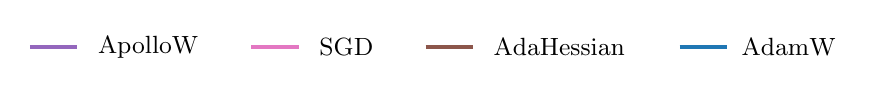
\begin{tikzpicture}[scale=0.75] % Nested TikZ environment
            \small 
            % AdaBelief
     \draw[mediumpurple148103189,  ultra thick] (0,0) -- ++(0.8,0);
     \node[anchor=west] at (1,0) {{ApolloW}}; % Increased spacing
     
     % Adam
    
     \draw[orchid227119194,  ultra thick] (3.75,0) -- ++(0.8,0);
     \node[anchor=west] at (4.75,0) {{SGD}}; % Increased spacing
     
     % AdaHessian
     \draw[sienna1408675,  ultra thick] (6.7,0) -- ++(0.8,0);
     \node[anchor=west] at (7.7,0) {{AdaHessian}}; % Increased spacing
     
     % Apollo
     \draw[steelblue31119180,  ultra thick] (11,0) -- ++(0.8,0);
     \node[anchor=west] at (11.9,0) {{AdamW}}; % Increased spacing
        
    \end{tikzpicture}
    };
    \end{tikzpicture}
     \\ 
    \end{tabular}
    \caption{Evaluation of optimizers on TinyImageNet using ResNet-18 with the \emph{milestone} learning rate scheduler, where hyperparameters
    are held constant across all optimizers}
    \label{fig:tinyimagenet-perf-milestone}
\end{figure}

As we can see in \ref{fig:tinyimagenet-perf-milestone} and \ref{fig:tinyimagenet-perf-cosine}, the performance of the second-order optimizers 
largely follows the same regime as in \ref{fig:cifar-10-milestone-real} and \ref{fig:cifar-10-milestone-second-best}. \emph{AdaHessian} and \emph{SGD} still aren't able to perform 
well with their non-optimal hyperparameters. Although it shows that they both have a steadily decreasing test loss, 
meaning they are able to prevent overfitting much better than \emph{AdamW} or \emph{AdaBelief}. 
Referring to \ref{fig:tinyimagenet-perf-opt}, we can see that \emph{AdaHessian} still shows a high amount of performance variance 
between its optimal and non-optimal hyperparameter settings, while \emph{Apollo} and \emph{ApolloW} have less variance in their performance. 
As both second-order methods are able to reduce the amount of overfitting, especially in the later epochs (100-120), and therefore 
achieve better generalization results, we could conclude that they are able to find flatter minima in the loss landscape, that
are generally associated with better generalization \cite{Goodfellow-et-al-2016}.
In terms of convergence behavior, we can see that although \emph{Apollo} and \emph{ApolloW} are able
to converge faster than \emph{AdaHessian}, they are still considerably slower than \emph{AdamW} and \emph{AdaBelief} (see \ref{tab:optimizer_comparison_ttc}). 
Therefore, we can conclude that, at least in its optimal setting, \emph{Apollo} is able to offer a reasonably good 
trade-off between convergence time and generalization performance. Meanwhile, \emph{AdaHessian} is severely limited in its practical 
applicability not only by its variability in performance, but also by its memory usage.

\begin{figure}[h!]
    \centering
    \begin{tabular}{cc}
        % This file was created with tikzplotlib v0.10.1.
\begin{tikzpicture}[scale=0.75]

    \definecolor{crimson2143940}{RGB}{214,39,40}
    \definecolor{darkgrey176}{RGB}{176,176,176}
    \definecolor{darkorange25512714}{RGB}{255,127,14}
    \definecolor{forestgreen4416044}{RGB}{44,160,44}
    \definecolor{grey127}{RGB}{127,127,127}
    \definecolor{lightgrey204}{RGB}{204,204,204}
    \definecolor{mediumpurple148103189}{RGB}{148,103,189}
    \definecolor{orchid227119194}{RGB}{227,119,194}
    \definecolor{sienna1408675}{RGB}{140,86,75}
    \definecolor{steelblue31119180}{RGB}{31,119,180}
    
    \begin{groupplot}[group style={group size=2 by 2,
        horizontal sep=1cm,  % Adjust horizontal spacing
        vertical sep=2cm}]
    \nextgroupplot[
    tick align=outside,
    tick pos=left,
    title={Polynom. Training Accuracy (milestone)},
    x grid style={darkgrey176},
    xlabel={Epochs},
    xmin=-5.95, xmax=124.95,
    xtick style={color=black},
    y grid style={darkgrey176},
    ymin=0.0058224104859335, ymax=1.04678708439898,
    ytick style={color=black}
    ]
    \addplot [semithick, steelblue31119180]
    table {%
    0 0.0919257512787724
    1 0.191460198209719
    2 0.253142982736573
    3 0.298677269820972
    4 0.335573849104859
    5 0.37102381713555
    6 0.400821211636829
    7 0.433072250639386
    8 0.461846627237852
    9 0.494455322890026
    10 0.523935022378517
    11 0.557730578644501
    12 0.589366208439898
    13 0.624724264705882
    14 0.661734734654731
    15 0.692475223785166
    16 0.726734335038363
    17 0.759968430306905
    18 0.788624920076726
    19 0.812192295396419
    20 0.830193014705882
    21 0.850075927109974
    22 0.860885549872123
    23 0.874666320332481
    24 0.887218270460358
    25 0.890644980818414
    26 0.899362611892583
    27 0.906078164961637
    28 0.908280051150895
    29 0.91346307544757
    30 0.920190617007673
    31 0.91974104859335
    32 0.925393622122762
    33 0.92890625
    34 0.929653532608696
    35 0.931683583759591
    36 0.930774456521739
    37 0.937410086317136
    38 0.941204443734015
    39 0.939044517263427
    40 0.972957960358056
    41 0.983667679028133
    42 0.987915601023018
    43 0.989765824808184
    44 0.99080682544757
    45 0.992669037723785
    46 0.993304427749361
    47 0.994089673913043
    48 0.99429347826087
    49 0.99524256713555
    50 0.99529851342711
    51 0.995558264066496
    52 0.996031809462916
    53 0.99626158887468
    54 0.996103740409207
    55 0.99610773657289
    56 0.996936940537084
    57 0.996677189897698
    58 0.997124760230179
    59 0.997230658567775
    60 0.997496403452685
    61 0.997334558823529
    62 0.997985933503836
    63 0.997532368925831
    64 0.997486413043478
    65 0.997806106138107
    66 0.99781010230179
    67 0.997686221227621
    68 0.997925991048593
    69 0.998149776214834
    70 0.998109814578005
    71 0.998131793478261
    72 0.998201726342711
    73 0.998035885549872
    74 0.998215712915601
    75 0.998201726342711
    76 0.998401534526854
    77 0.998501438618926
    78 0.998245684143222
    79 0.99866128516624
    80 0.998805147058824
    81 0.998595348465473
    82 0.998865089514066
    83 0.999074888107417
    84 0.998945012787724
    85 0.998851102941177
    86 0.999000959079284
    87 0.999070891943734
    88 0.99898097826087
    89 0.999084878516624
    90 0.999014945652174
    91 0.999090872762148
    92 0.999210757672634
    93 0.999150815217391
    94 0.999150815217391
    95 0.999070891943734
    96 0.999214753836317
    97 0.999280690537084
    98 0.999144820971867
    99 0.999290680946292
    100 0.999150815217391
    101 0.999290680946292
    102 0.999270700127877
    103 0.999310661764706
    104 0.999268702046036
    105 0.99940057544757
    106 0.999150815217391
    107 0.99926070971867
    108 0.999410565856777
    109 0.999294677109974
    110 0.999374600383632
    111 0.999370604219949
    112 0.999230738491049
    113 0.999370604219949
    114 0.99933064258312
    115 0.99926070971867
    116 0.999340632992327
    117 0.999310661764706
    118 0.999304667519182
    119 0.99947050831202
    };
    \addplot [semithick, darkorange25512714]
    table {%
    0 0.0898277653452685
    1 0.19065297314578
    2 0.245352461636829
    3 0.285140265345269
    4 0.318328404731458
    5 0.346793078644501
    6 0.373673273657289
    7 0.397985933503836
    8 0.4209538842711
    9 0.441761908567775
    10 0.461940537084399
    11 0.484966432225064
    12 0.503872282608696
    13 0.521429427749361
    14 0.545406409846547
    15 0.562210278132992
    16 0.583172154731458
    17 0.601742327365729
    18 0.618276454603581
    19 0.635136269181586
    20 0.650691336317135
    21 0.667946771099744
    22 0.686880594629156
    23 0.697983935421995
    24 0.71499760230179
    25 0.725799232736573
    26 0.734790601023018
    27 0.746129715473146
    28 0.759740648976982
    29 0.762565936700767
    30 0.774410565856777
    31 0.781060182225064
    32 0.786185262148338
    33 0.79600983056266
    34 0.798285645780051
    35 0.802803308823529
    36 0.811702765345269
    37 0.813207320971867
    38 0.81657408887468
    39 0.819938858695652
    40 0.90803628516624
    41 0.937222266624041
    42 0.949352621483376
    43 0.956435821611253
    44 0.963860693734015
    45 0.967459239130435
    46 0.971173673273657
    47 0.973509430946291
    48 0.976292758951407
    49 0.977609494884911
    50 0.979591592071611
    51 0.980554667519182
    52 0.982940377237852
    53 0.983561780690537
    54 0.983501838235294
    55 0.985625799232737
    56 0.986271179667519
    57 0.98614729859335
    58 0.987645859974424
    59 0.987689817774936
    60 0.987827685421995
    61 0.989334239130435
    62 0.989106457800512
    63 0.989440137468031
    64 0.989232336956522
    65 0.989849744245524
    66 0.990377237851662
    67 0.990692934782609
    68 0.99044317455243
    69 0.990579044117647
    70 0.991370284526854
    71 0.991022618286445
    72 0.99164402173913
    73 0.991484175191816
    74 0.991470188618926
    75 0.992167519181586
    76 0.99220148657289
    77 0.992221467391304
    78 0.99203364769821
    79 0.992449248721228
    80 0.993985773657289
    81 0.994383391943734
    82 0.995348465473146
    83 0.99528452685422
    84 0.995282528772379
    85 0.995937899616368
    86 0.996215632992327
    87 0.996101742327366
    88 0.996207640664962
    89 0.996595268542199
    90 0.996697170716113
    91 0.996597266624041
    92 0.996873001918159
    93 0.997006873401534
    94 0.997036844629156
    95 0.996910965473146
    96 0.997094789002558
    97 0.997102781329923
    98 0.997326566496164
    99 0.99744645140665
    100 0.997230658567775
    101 0.997336556905371
    102 0.997672234654731
    103 0.997532368925831
    104 0.997732177109974
    105 0.997756154092072
    106 0.997138746803069
    107 0.997536365089514
    108 0.997486413043478
    109 0.997720188618926
    110 0.997846067774936
    111 0.99764226342711
    112 0.99778212915601
    113 0.997961956521739
    114 0.997981937340154
    115 0.997872042838875
    116 0.997756154092072
    117 0.997850063938619
    118 0.997995923913043
    119 0.998041879795396
    };
    \addplot [semithick, forestgreen4416044]
    table {%
    0 0.0906869405370844
    1 0.190884750639386
    2 0.249306665601023
    3 0.297904012148338
    4 0.334448929028133
    5 0.368090632992327
    6 0.399508471867008
    7 0.429829363810742
    8 0.462484015345269
    9 0.494073689258312
    10 0.523183743606138
    11 0.554307864450128
    12 0.589504076086957
    13 0.621103740409207
    14 0.659778612531969
    15 0.694453324808184
    16 0.7279851342711
    17 0.756090153452685
    18 0.785234175191816
    19 0.810032368925831
    20 0.829959239130435
    21 0.847981937340153
    22 0.861790680946292
    23 0.872748161764706
    24 0.882346946930946
    25 0.890189418158568
    26 0.899608375959079
    27 0.903644501278772
    28 0.90803628516624
    29 0.916438219309463
    30 0.913772778132992
    31 0.91856817455243
    32 0.924182784526854
    33 0.928776374680307
    34 0.930800431585678
    35 0.932362931585678
    36 0.934860533887468
    37 0.935889546035806
    38 0.937719789002558
    39 0.939859734654731
    40 0.97240449168798
    41 0.982576726342711
    42 0.987462036445013
    43 0.989735853580563
    44 0.991272378516624
    45 0.992671035805627
    46 0.992746962915601
    47 0.993394341432225
    48 0.994173593350384
    49 0.995064737851662
    50 0.995408407928389
    51 0.995684143222506
    52 0.995977861253197
    53 0.996281569693095
    54 0.996063778772379
    55 0.996427429667519
    56 0.996533328005115
    57 0.997274616368286
    58 0.997174712276215
    59 0.996876998081841
    60 0.996996882992327
    61 0.997406489769821
    62 0.997504395780051
    63 0.997476422634271
    64 0.997466432225064
    65 0.997732177109974
    66 0.997646259590793
    67 0.997896019820972
    68 0.997626278772378
    69 0.998021898976982
    70 0.997921994884911
    71 0.997931985294118
    72 0.997951966112532
    73 0.997949968030691
    74 0.998101822250639
    75 0.997906010230179
    76 0.998121803069054
    77 0.998181745524297
    78 0.998155770460358
    79 0.99866128516624
    80 0.99845148657289
    81 0.998865089514066
    82 0.998851102941177
    83 0.998990968670077
    84 0.999020939897698
    85 0.999060901534527
    86 0.999114849744245
    87 0.999110853580563
    88 0.998921035805627
    89 0.999100863171355
    90 0.99905091112532
    91 0.998960997442455
    92 0.999170796035806
    93 0.999094868925831
    94 0.999244725063939
    95 0.999284686700767
    96 0.99912084398977
    97 0.999278692455243
    98 0.99919077685422
    99 0.999180786445013
    100 0.999158807544757
    101 0.99919077685422
    102 0.999210757672634
    103 0.999280690537084
    104 0.999320652173913
    105 0.999304667519182
    106 0.999270700127877
    107 0.999380594629156
    108 0.99933064258312
    109 0.99928868286445
    110 0.999350623401535
    111 0.99926070971867
    112 0.999370604219949
    113 0.999360613810742
    114 0.999240728900256
    115 0.999430546675192
    116 0.999290680946292
    117 0.99933064258312
    118 0.999350623401535
    119 0.999310661764706
    };
    \addplot [semithick, crimson2143940]
    table {%
    0 0.0558563778772379
    1 0.156811460997442
    2 0.22882233056266
    3 0.278708439897698
    4 0.320676150895141
    5 0.353288842710997
    6 0.382161125319693
    7 0.410697730179028
    8 0.436598865089514
    9 0.461217231457801
    10 0.482492806905371
    11 0.505298913043478
    12 0.528980179028133
    13 0.552253836317136
    14 0.571954923273657
    15 0.591044597186701
    16 0.611003436700767
    17 0.632816496163683
    18 0.653426710358056
    19 0.673111812659847
    20 0.68888067455243
    21 0.703632512787724
    22 0.723739210358056
    23 0.739498081841432
    24 0.752281809462916
    25 0.770178628516624
    26 0.778160965473146
    27 0.791250399616368
    28 0.800305706521739
    29 0.809948449488491
    30 0.816779891304348
    31 0.823883072250639
    32 0.834876518542199
    33 0.841905770460358
    34 0.843953804347826
    35 0.851216831841432
    36 0.852048033887468
    37 0.858771579283887
    38 0.863704843350384
    39 0.861015425191816
    40 0.946007832480818
    41 0.972856058184143
    42 0.979863331202046
    43 0.983781569693095
    44 0.986534926470588
    45 0.987957560741688
    46 0.99052709398977
    47 0.9907648657289
    48 0.99206162084399
    49 0.992601102941176
    50 0.993817934782609
    51 0.993869884910486
    52 0.99440537084399
    53 0.994942854859335
    54 0.994834958439898
    55 0.995432384910486
    56 0.995642183503836
    57 0.996147698209719
    58 0.996221627237852
    59 0.996237611892583
    60 0.996587276214834
    61 0.996537324168798
    62 0.996827046035806
    63 0.99712675831202
    64 0.997072810102302
    65 0.997552349744246
    66 0.997752157928389
    67 0.997676230818414
    68 0.997582320971867
    69 0.997906010230179
    70 0.997836077365729
    71 0.997971946930946
    72 0.997802109974425
    73 0.998355578644501
    74 0.998111812659846
    75 0.997981937340154
    76 0.998081841432225
    77 0.998385549872123
    78 0.998461476982097
    79 0.998281649616368
    80 0.998571371483376
    81 0.998751198849105
    82 0.99859135230179
    83 0.998711237212276
    84 0.998411524936061
    85 0.998845108695652
    86 0.998705242966752
    87 0.998681265984655
    88 0.998831122122762
    89 0.998861093350384
    90 0.998811141304348
    91 0.998755195012788
    92 0.998831122122762
    93 0.998921035805627
    94 0.998871083759591
    95 0.998681265984655
    96 0.998805147058824
    97 0.998655290920716
    98 0.998841112531969
    99 0.998851102941177
    100 0.998781170076726
    101 0.998861093350384
    102 0.998791160485934
    103 0.998755195012788
    104 0.998831122122762
    105 0.999080882352941
    106 0.998825127877238
    107 0.998831122122762
    108 0.99898097826087
    109 0.998829124040921
    110 0.998931026214834
    111 0.999130834398977
    112 0.998990968670077
    113 0.998789162404092
    114 0.999130834398977
    115 0.998935022378517
    116 0.998960997442455
    117 0.998941016624041
    118 0.998970987851662
    119 0.998941016624041
    };
    \addplot [semithick, mediumpurple148103189]
    table {%
    0 0.056074168797954
    1 0.156497762148338
    2 0.229635549872123
    3 0.279108056265985
    4 0.315363251278772
    5 0.349210757672634
    6 0.37756753516624
    7 0.404713475063939
    8 0.428364769820972
    9 0.453174952046036
    10 0.477993126598465
    11 0.498433503836317
    12 0.520000799232737
    13 0.542888826726343
    14 0.564372202685422
    15 0.583859494884911
    16 0.60319493286445
    17 0.623075847186701
    18 0.646297554347826
    19 0.659798593350384
    20 0.681533727621483
    21 0.699160805626598
    22 0.71243006713555
    23 0.72811101342711
    24 0.744858935421995
    25 0.756963315217391
    26 0.767892822890026
    27 0.780766464194373
    28 0.790317295396419
    29 0.80076726342711
    30 0.808164162404092
    31 0.818510230179028
    32 0.823259670716113
    33 0.83056665601023
    34 0.833359974424552
    35 0.843382352941176
    36 0.847212675831202
    37 0.851636429028133
    38 0.855023177749361
    39 0.854112052429667
    40 0.940942695012788
    41 0.970774056905371
    42 0.978742407289003
    43 0.982418877877238
    44 0.985094309462916
    45 0.987817695012788
    46 0.989933663682864
    47 0.990501118925831
    48 0.991028612531969
    49 0.992770939897698
    50 0.992918797953964
    51 0.993815936700767
    52 0.99441935741688
    53 0.994435342071611
    54 0.995044757033248
    55 0.995344469309463
    56 0.995867966751918
    57 0.995845987851662
    58 0.995909926470588
    59 0.996207640664962
    60 0.996349504475703
    61 0.996837036445013
    62 0.996853021099744
    63 0.997256633631713
    64 0.996984894501279
    65 0.997092790920716
    66 0.997506393861893
    67 0.997326566496164
    68 0.997580322890026
    69 0.997792119565217
    70 0.997650255754476
    71 0.998231697570332
    72 0.997989929667519
    73 0.998051870204604
    74 0.998075847186701
    75 0.998191735933504
    76 0.99824168797954
    77 0.998495444373401
    78 0.998531409846547
    79 0.99852141943734
    80 0.998691256393862
    81 0.998601342710997
    82 0.998471467391304
    83 0.998699248721228
    84 0.998735214194373
    85 0.998781170076726
    86 0.998711237212276
    87 0.998659287084399
    88 0.998561381074169
    89 0.998821131713555
    90 0.998641304347826
    91 0.998651294757033
    92 0.998801150895141
    93 0.998645300511509
    94 0.998669277493606
    95 0.998795156649616
    96 0.998741208439898
    97 0.998789162404092
    98 0.998960997442455
    99 0.998711237212276
    100 0.998861093350384
    101 0.998741208439898
    102 0.998651294757033
    103 0.998771179667519
    104 0.998745204603581
    105 0.998751198849105
    106 0.99898097826087
    107 0.998925031969309
    108 0.998925031969309
    109 0.998725223785166
    110 0.998701246803069
    111 0.998931026214834
    112 0.999010949488491
    113 0.998865089514066
    114 0.998895060741688
    115 0.998951007033248
    116 0.999030930306905
    117 0.999020939897698
    118 0.999160805626598
    119 0.998641304347826
    };
    \addplot [semithick, sienna1408675]
    table {%
    0 0.0583240089514067
    1 0.154875319693095
    2 0.222288602941176
    3 0.268462276214834
    4 0.302044037723785
    5 0.331279971227622
    6 0.358653692455243
    7 0.383240089514067
    8 0.401640425191816
    9 0.421709159207161
    10 0.438049472506394
    11 0.453648497442455
    12 0.465333280051151
    13 0.480093110613811
    14 0.489236333120205
    15 0.500399616368286
    16 0.512146339514067
    17 0.521007832480818
    18 0.533324008951407
    19 0.540724904092072
    20 0.549678308823529
    21 0.557668638107417
    22 0.564092471227622
    23 0.572292599104859
    24 0.58214314258312
    25 0.589320252557545
    26 0.597706202046036
    27 0.60710118286445
    28 0.614631953324808
    29 0.622736173273657
    30 0.628468670076726
    31 0.636936540920716
    32 0.642699008951407
    33 0.64774016943734
    34 0.656719549232737
    35 0.661239210358056
    36 0.665984654731458
    37 0.673749200767264
    38 0.680414801790281
    39 0.684752637468031
    40 0.848639306265985
    41 0.906050191815857
    42 0.927561540920716
    43 0.942181505754476
    44 0.951224824168798
    45 0.958587755754476
    46 0.964354219948849
    47 0.968797953964194
    48 0.972760150255754
    49 0.974998001918159
    50 0.978214913682864
    51 0.981132113171355
    52 0.982005274936061
    53 0.982820492327366
    54 0.984426950127877
    55 0.985791640025576
    56 0.986582880434783
    57 0.987466032608696
    58 0.989114450127877
    59 0.989394181585678
    60 0.989907688618926
    61 0.990267343350384
    62 0.990846787084399
    63 0.991460198209719
    64 0.99221547314578
    65 0.992840872762148
    66 0.992776934143223
    67 0.993795955882353
    68 0.993480258951407
    69 0.993853900255754
    70 0.993644101662404
    71 0.994353420716113
    72 0.994239530051151
    73 0.994395380434783
    74 0.99476902173913
    75 0.995268542199488
    76 0.995608216112532
    77 0.995712116368286
    78 0.995212595907928
    79 0.995768062659847
    80 0.996265585038363
    81 0.996801070971867
    82 0.997090792838875
    83 0.997002877237852
    84 0.997596307544757
    85 0.997386508951407
    86 0.997562340153453
    87 0.99757233056266
    88 0.997616288363171
    89 0.997602301790281
    90 0.99771219629156
    91 0.997842071611253
    92 0.997732177109974
    93 0.99778212915601
    94 0.997916000639386
    95 0.997971946930946
    96 0.998205722506394
    97 0.998085837595908
    98 0.997822090792839
    99 0.997965952685422
    100 0.99824168797954
    101 0.997906010230179
    102 0.998361572890026
    103 0.998081841432225
    104 0.998341592071611
    105 0.998125799232736
    106 0.998285645780051
    107 0.998335597826087
    108 0.998375559462916
    109 0.998351582480818
    110 0.998351582480818
    111 0.998361572890026
    112 0.998399536445013
    113 0.998471467391304
    114 0.998495444373401
    115 0.998525415601023
    116 0.998485453964194
    117 0.998485453964194
    118 0.99845148657289
    119 0.99867527173913
    };
    \addplot [semithick, orchid227119194]
    table {%
    0 0.0534127237851662
    1 0.136015425191816
    2 0.193779971227621
    3 0.233611732736573
    4 0.268078644501279
    5 0.293999760230179
    6 0.320650175831202
    7 0.344199568414322
    8 0.368454283887468
    9 0.390029571611253
    10 0.410475943094629
    11 0.432324968030691
    12 0.452945172634271
    13 0.47520979859335
    14 0.495782049232737
    15 0.518288443094629
    16 0.537629875319693
    17 0.559842551150895
    18 0.578810342071611
    19 0.60062739769821
    20 0.624788203324808
    21 0.640880754475703
    22 0.664004555626598
    23 0.686197250639386
    24 0.705432784526854
    25 0.728944213554987
    26 0.745786045396419
    27 0.76421635230179
    28 0.781595668158568
    29 0.801015025575447
    30 0.815816815856777
    31 0.829291879795396
    32 0.847046835038363
    33 0.859732656649616
    34 0.868002717391304
    35 0.879010150255754
    36 0.8887827685422
    37 0.899408567774936
    38 0.908779571611253
    39 0.91111932544757
    40 0.958401934143223
    41 0.972580322890025
    42 0.976914162404092
    43 0.98023097826087
    44 0.981084159207161
    45 0.98263067455243
    46 0.983419916879795
    47 0.985136269181586
    48 0.986666799872123
    49 0.987210278132992
    50 0.988465073529412
    51 0.988425111892583
    52 0.989186381074169
    53 0.988974584398977
    54 0.990245364450128
    55 0.990670955882353
    56 0.991382273017903
    57 0.990521099744246
    58 0.991719948849105
    59 0.991879795396419
    60 0.991777893222506
    61 0.992661045396419
    62 0.992647058823529
    63 0.992966751918159
    64 0.993018702046036
    65 0.993194533248082
    66 0.993428308823529
    67 0.994003756393862
    68 0.993742007672634
    69 0.993929827365729
    70 0.994099664322251
    71 0.994549232736573
    72 0.994003756393862
    73 0.99462915601023
    74 0.994603180946292
    75 0.994808983375959
    76 0.995118686061381
    77 0.994922874040921
    78 0.995134670716113
    79 0.995236572890026
    80 0.9958140185422
    81 0.995518302429667
    82 0.995638187340153
    83 0.995845987851662
    84 0.995837995524297
    85 0.995744085677749
    86 0.995879955242967
    87 0.995891943734015
    88 0.995808024296675
    89 0.995768062659847
    90 0.99602381713555
    91 0.995877957161125
    92 0.996033807544757
    93 0.996015824808184
    94 0.995534287084399
    95 0.996011828644501
    96 0.995891943734015
    97 0.996277573529412
    98 0.995887947570332
    99 0.9958140185422
    100 0.995744085677749
    101 0.995917918797954
    102 0.995857976342711
    103 0.995867966751918
    104 0.996013826726343
    105 0.996101742327366
    106 0.996253596547315
    107 0.996147698209719
    108 0.996101742327366
    109 0.996147698209719
    110 0.995927909207161
    111 0.996007832480818
    112 0.996277573529412
    113 0.996367487212276
    114 0.996127717391304
    115 0.996497362531969
    116 0.996287563938619
    117 0.996173673273657
    118 0.996597266624041
    119 0.996027813299233
    };
    \addplot [semithick, grey127]
    table {%
    0 0.05313898657289
    1 0.146457400895141
    2 0.210244165601023
    3 0.258903452685422
    4 0.297052829283887
    5 0.334504875319693
    6 0.366815856777494
    7 0.39920476342711
    8 0.428192934782609
    9 0.456625639386189
    10 0.487943574168798
    11 0.521153692455243
    12 0.553316815856777
    13 0.591727941176471
    14 0.624052909207161
    15 0.659135230179028
    16 0.691987691815857
    17 0.724270700127877
    18 0.754415760869565
    19 0.778862292199488
    20 0.803552589514066
    21 0.822788123401535
    22 0.839482097186701
    23 0.85246962915601
    24 0.868128596547315
    25 0.875997042838875
    26 0.885342071611253
    27 0.891907768542199
    28 0.898972985933504
    29 0.906160086317136
    30 0.911081361892583
    31 0.914587995524297
    32 0.918586157289003
    33 0.920951886189258
    34 0.925881154092072
    35 0.928454683503836
    36 0.930948289641944
    37 0.934508871483376
    38 0.937180306905371
    39 0.938702845268542
    40 0.972100783248082
    41 0.983833519820972
    42 0.988411125319693
    43 0.990361253196931
    44 0.992127557544757
    45 0.992371323529412
    46 0.99351222826087
    47 0.994639146419437
    48 0.994065696930946
    49 0.994838954603581
    50 0.995644181585678
    51 0.996085757672634
    52 0.99582800511509
    53 0.996383471867008
    54 0.996557304987212
    55 0.996717151534527
    56 0.996942934782609
    57 0.997366528132992
    58 0.997170716112532
    59 0.997286604859335
    60 0.997212675831202
    61 0.997596307544757
    62 0.99743246483376
    63 0.997706202046036
    64 0.997786125319693
    65 0.997886029411765
    66 0.997732177109974
    67 0.99786604859335
    68 0.998041879795396
    69 0.998061860613811
    70 0.997925991048593
    71 0.997975943094629
    72 0.997870044757033
    73 0.998115808823529
    74 0.998221707161125
    75 0.998193734015345
    76 0.998651294757033
    77 0.998195732097187
    78 0.998251678388747
    79 0.998261668797954
    80 0.998645300511509
    81 0.998625319693095
    82 0.998801150895141
    83 0.998970987851662
    84 0.998871083759591
    85 0.999060901534527
    86 0.998881074168798
    87 0.999030930306905
    88 0.998990968670077
    89 0.99905091112532
    90 0.999024936061381
    91 0.999020939897698
    92 0.999060901534527
    93 0.999140824808184
    94 0.999060901534527
    95 0.998941016624041
    96 0.999170796035806
    97 0.998990968670077
    98 0.999070891943734
    99 0.999110853580563
    100 0.99920476342711
    101 0.999170796035806
    102 0.99905091112532
    103 0.999290680946292
    104 0.999380594629156
    105 0.999220748081841
    106 0.999350623401535
    107 0.999180786445013
    108 0.999130834398977
    109 0.999320652173913
    110 0.999170796035806
    111 0.999244725063939
    112 0.999118845907928
    113 0.999280690537084
    114 0.99933064258312
    115 0.999284686700767
    116 0.99926070971867
    117 0.999230738491049
    118 0.999254715473146
    119 0.999390585038363
    };
    
    \nextgroupplot[
    tick align=outside,
    tick pos=left,
    title={Polynom. Test Accuracy (milestone)},
    x grid style={darkgrey176},
    xlabel={Epochs},
    xmin=-5.95, xmax=124.95,
    xtick style={color=black},
    y grid style={darkgrey176},
    ymin=0.07841796875, ymax=0.46728515625,
    ytick style={color=black}
    ]
    \addplot [semithick, steelblue31119180]
    table {%
    0 0.141015625
    1 0.206640625
    2 0.26044921875
    3 0.29189453125
    4 0.33046875
    5 0.334375
    6 0.3734375
    7 0.38095703125
    8 0.381640625
    9 0.37998046875
    10 0.38828125
    11 0.3943359375
    12 0.39033203125
    13 0.4076171875
    14 0.3970703125
    15 0.3986328125
    16 0.39833984375
    17 0.38671875
    18 0.38369140625
    19 0.384375
    20 0.38857421875
    21 0.38447265625
    22 0.38544921875
    23 0.3818359375
    24 0.38330078125
    25 0.3755859375
    26 0.38837890625
    27 0.3875
    28 0.38154296875
    29 0.3802734375
    30 0.37607421875
    31 0.37919921875
    32 0.38564453125
    33 0.391015625
    34 0.382421875
    35 0.36884765625
    36 0.38359375
    37 0.38603515625
    38 0.3826171875
    39 0.38232421875
    40 0.40556640625
    41 0.4080078125
    42 0.40888671875
    43 0.409765625
    44 0.41162109375
    45 0.41513671875
    46 0.41396484375
    47 0.411328125
    48 0.4177734375
    49 0.4154296875
    50 0.4158203125
    51 0.4162109375
    52 0.41845703125
    53 0.4126953125
    54 0.40986328125
    55 0.4140625
    56 0.41630859375
    57 0.41328125
    58 0.41259765625
    59 0.4134765625
    60 0.4171875
    61 0.4177734375
    62 0.41474609375
    63 0.4140625
    64 0.41064453125
    65 0.4134765625
    66 0.41474609375
    67 0.41494140625
    68 0.41708984375
    69 0.41484375
    70 0.41484375
    71 0.41708984375
    72 0.4150390625
    73 0.41572265625
    74 0.414453125
    75 0.41455078125
    76 0.41240234375
    77 0.412890625
    78 0.41513671875
    79 0.41337890625
    80 0.41123046875
    81 0.41103515625
    82 0.41298828125
    83 0.41474609375
    84 0.415234375
    85 0.415625
    86 0.41484375
    87 0.4162109375
    88 0.4171875
    89 0.41884765625
    90 0.41591796875
    91 0.416015625
    92 0.4177734375
    93 0.418359375
    94 0.416015625
    95 0.41552734375
    96 0.41806640625
    97 0.41689453125
    98 0.4181640625
    99 0.41806640625
    100 0.41669921875
    101 0.41923828125
    102 0.41865234375
    103 0.419140625
    104 0.4189453125
    105 0.4181640625
    106 0.41826171875
    107 0.4171875
    108 0.41796875
    109 0.41875
    110 0.41904296875
    111 0.42001953125
    112 0.41904296875
    113 0.419140625
    114 0.4201171875
    115 0.4216796875
    116 0.41884765625
    117 0.4197265625
    118 0.42001953125
    119 0.42001953125
    };
    \addplot [semithick, darkorange25512714]
    table {%
    0 0.14130859375
    1 0.21884765625
    2 0.253515625
    3 0.29658203125
    4 0.29931640625
    5 0.31396484375
    6 0.347265625
    7 0.35439453125
    8 0.3765625
    9 0.360546875
    10 0.3931640625
    11 0.3947265625
    12 0.39375
    13 0.39140625
    14 0.39580078125
    15 0.42158203125
    16 0.4169921875
    17 0.41376953125
    18 0.4140625
    19 0.41005859375
    20 0.4060546875
    21 0.4095703125
    22 0.39921875
    23 0.40400390625
    24 0.40009765625
    25 0.40458984375
    26 0.38916015625
    27 0.3939453125
    28 0.3865234375
    29 0.389453125
    30 0.39150390625
    31 0.3900390625
    32 0.40009765625
    33 0.3947265625
    34 0.39619140625
    35 0.4
    36 0.3978515625
    37 0.3958984375
    38 0.39755859375
    39 0.39609375
    40 0.424609375
    41 0.42939453125
    42 0.430859375
    43 0.43154296875
    44 0.4306640625
    45 0.4318359375
    46 0.43193359375
    47 0.42998046875
    48 0.43095703125
    49 0.43115234375
    50 0.42939453125
    51 0.43232421875
    52 0.42978515625
    53 0.42958984375
    54 0.43291015625
    55 0.43330078125
    56 0.43271484375
    57 0.4359375
    58 0.43271484375
    59 0.42724609375
    60 0.42939453125
    61 0.429296875
    62 0.42890625
    63 0.42861328125
    64 0.428125
    65 0.43056640625
    66 0.4279296875
    67 0.43134765625
    68 0.429296875
    69 0.42607421875
    70 0.429296875
    71 0.43017578125
    72 0.4255859375
    73 0.42744140625
    74 0.4275390625
    75 0.42900390625
    76 0.4251953125
    77 0.4283203125
    78 0.4259765625
    79 0.425390625
    80 0.42578125
    81 0.430078125
    82 0.4279296875
    83 0.431640625
    84 0.427734375
    85 0.42890625
    86 0.430859375
    87 0.43125
    88 0.4279296875
    89 0.428125
    90 0.43203125
    91 0.43017578125
    92 0.42890625
    93 0.4310546875
    94 0.43154296875
    95 0.4279296875
    96 0.42958984375
    97 0.43056640625
    98 0.43115234375
    99 0.43056640625
    100 0.43173828125
    101 0.43193359375
    102 0.428125
    103 0.42958984375
    104 0.430078125
    105 0.4291015625
    106 0.43095703125
    107 0.4314453125
    108 0.430859375
    109 0.4287109375
    110 0.430078125
    111 0.43017578125
    112 0.43037109375
    113 0.42880859375
    114 0.43095703125
    115 0.43154296875
    116 0.43056640625
    117 0.43017578125
    118 0.43056640625
    119 0.43056640625
    };
    \addplot [semithick, forestgreen4416044]
    table {%
    0 0.16103515625
    1 0.23095703125
    2 0.27177734375
    3 0.2984375
    4 0.3341796875
    5 0.33798828125
    6 0.3455078125
    7 0.3720703125
    8 0.387890625
    9 0.38349609375
    10 0.395703125
    11 0.394140625
    12 0.40068359375
    13 0.39150390625
    14 0.40908203125
    15 0.3974609375
    16 0.39990234375
    17 0.39638671875
    18 0.38974609375
    19 0.3884765625
    20 0.38759765625
    21 0.385546875
    22 0.3958984375
    23 0.38447265625
    24 0.38212890625
    25 0.3931640625
    26 0.3828125
    27 0.3806640625
    28 0.373046875
    29 0.37666015625
    30 0.3853515625
    31 0.3759765625
    32 0.38701171875
    33 0.387890625
    34 0.37880859375
    35 0.388671875
    36 0.3796875
    37 0.36611328125
    38 0.383203125
    39 0.38173828125
    40 0.40673828125
    41 0.409765625
    42 0.4115234375
    43 0.4111328125
    44 0.41240234375
    45 0.41376953125
    46 0.41240234375
    47 0.4130859375
    48 0.415625
    49 0.41533203125
    50 0.4150390625
    51 0.41669921875
    52 0.41611328125
    53 0.4169921875
    54 0.4146484375
    55 0.4115234375
    56 0.41513671875
    57 0.41298828125
    58 0.412109375
    59 0.41650390625
    60 0.41103515625
    61 0.414453125
    62 0.4158203125
    63 0.4140625
    64 0.4166015625
    65 0.41650390625
    66 0.4177734375
    67 0.41630859375
    68 0.41748046875
    69 0.4189453125
    70 0.41513671875
    71 0.41611328125
    72 0.41728515625
    73 0.41708984375
    74 0.4146484375
    75 0.4181640625
    76 0.4158203125
    77 0.4169921875
    78 0.41611328125
    79 0.41865234375
    80 0.41748046875
    81 0.41962890625
    82 0.4201171875
    83 0.41787109375
    84 0.42021484375
    85 0.41806640625
    86 0.4181640625
    87 0.419921875
    88 0.41962890625
    89 0.42080078125
    90 0.42041015625
    91 0.42158203125
    92 0.4201171875
    93 0.4212890625
    94 0.42197265625
    95 0.419140625
    96 0.420703125
    97 0.419921875
    98 0.41865234375
    99 0.41845703125
    100 0.4189453125
    101 0.41923828125
    102 0.41884765625
    103 0.419921875
    104 0.42109375
    105 0.41845703125
    106 0.41962890625
    107 0.42021484375
    108 0.4189453125
    109 0.42060546875
    110 0.42041015625
    111 0.41943359375
    112 0.4197265625
    113 0.419921875
    114 0.4203125
    115 0.419140625
    116 0.41943359375
    117 0.4185546875
    118 0.41953125
    119 0.41884765625
    };
    \addplot [semithick, crimson2143940]
    table {%
    0 0.1076171875
    1 0.19580078125
    2 0.234765625
    3 0.28291015625
    4 0.303515625
    5 0.34208984375
    6 0.35029296875
    7 0.35322265625
    8 0.3708984375
    9 0.380078125
    10 0.388671875
    11 0.3837890625
    12 0.37666015625
    13 0.3884765625
    14 0.3908203125
    15 0.39619140625
    16 0.393359375
    17 0.3732421875
    18 0.389453125
    19 0.4025390625
    20 0.3841796875
    21 0.37451171875
    22 0.3876953125
    23 0.38330078125
    24 0.38203125
    25 0.38798828125
    26 0.3783203125
    27 0.3900390625
    28 0.38447265625
    29 0.37978515625
    30 0.38251953125
    31 0.3859375
    32 0.3841796875
    33 0.38701171875
    34 0.380078125
    35 0.380078125
    36 0.38662109375
    37 0.37861328125
    38 0.37958984375
    39 0.3828125
    40 0.428125
    41 0.431640625
    42 0.4328125
    43 0.4349609375
    44 0.4359375
    45 0.4375
    46 0.43740234375
    47 0.439453125
    48 0.4376953125
    49 0.4384765625
    50 0.4365234375
    51 0.4390625
    52 0.43955078125
    53 0.43935546875
    54 0.43955078125
    55 0.44189453125
    56 0.44091796875
    57 0.44140625
    58 0.44150390625
    59 0.44140625
    60 0.4423828125
    61 0.4396484375
    62 0.44296875
    63 0.4408203125
    64 0.44111328125
    65 0.44189453125
    66 0.44326171875
    67 0.44208984375
    68 0.44287109375
    69 0.440625
    70 0.44208984375
    71 0.4421875
    72 0.44091796875
    73 0.44423828125
    74 0.446875
    75 0.445703125
    76 0.4421875
    77 0.44501953125
    78 0.44560546875
    79 0.4451171875
    80 0.44677734375
    81 0.4466796875
    82 0.445703125
    83 0.44384765625
    84 0.446484375
    85 0.44521484375
    86 0.4466796875
    87 0.44638671875
    88 0.447265625
    89 0.4462890625
    90 0.4455078125
    91 0.44541015625
    92 0.44443359375
    93 0.4462890625
    94 0.4470703125
    95 0.446484375
    96 0.4462890625
    97 0.44873046875
    98 0.4462890625
    99 0.44541015625
    100 0.4431640625
    101 0.4451171875
    102 0.446484375
    103 0.44541015625
    104 0.44755859375
    105 0.44580078125
    106 0.4466796875
    107 0.4470703125
    108 0.4458984375
    109 0.44541015625
    110 0.444140625
    111 0.4458984375
    112 0.44697265625
    113 0.44697265625
    114 0.44638671875
    115 0.44794921875
    116 0.44912109375
    117 0.4439453125
    118 0.44873046875
    119 0.449609375
    };
    \addplot [semithick, mediumpurple148103189]
    table {%
    0 0.09697265625
    1 0.18642578125
    2 0.2693359375
    3 0.28203125
    4 0.27998046875
    5 0.3208984375
    6 0.31494140625
    7 0.348046875
    8 0.35107421875
    9 0.36328125
    10 0.3576171875
    11 0.3751953125
    12 0.3728515625
    13 0.3783203125
    14 0.3755859375
    15 0.3888671875
    16 0.3828125
    17 0.38466796875
    18 0.38818359375
    19 0.3759765625
    20 0.37294921875
    21 0.375
    22 0.38525390625
    23 0.36259765625
    24 0.3740234375
    25 0.36630859375
    26 0.37138671875
    27 0.373046875
    28 0.3716796875
    29 0.3736328125
    30 0.3544921875
    31 0.375
    32 0.35107421875
    33 0.37958984375
    34 0.36884765625
    35 0.3673828125
    36 0.37216796875
    37 0.3671875
    38 0.36279296875
    39 0.36279296875
    40 0.4154296875
    41 0.42236328125
    42 0.41953125
    43 0.42373046875
    44 0.42333984375
    45 0.4259765625
    46 0.4248046875
    47 0.4240234375
    48 0.42529296875
    49 0.42333984375
    50 0.42529296875
    51 0.42568359375
    52 0.42548828125
    53 0.4291015625
    54 0.42548828125
    55 0.430078125
    56 0.42900390625
    57 0.4275390625
    58 0.42861328125
    59 0.42939453125
    60 0.42841796875
    61 0.42431640625
    62 0.42998046875
    63 0.42939453125
    64 0.428125
    65 0.429296875
    66 0.42890625
    67 0.4265625
    68 0.4287109375
    69 0.427734375
    70 0.42490234375
    71 0.42431640625
    72 0.42646484375
    73 0.42890625
    74 0.43271484375
    75 0.43095703125
    76 0.430078125
    77 0.43134765625
    78 0.42958984375
    79 0.43212890625
    80 0.42939453125
    81 0.432421875
    82 0.43134765625
    83 0.4298828125
    84 0.42958984375
    85 0.42998046875
    86 0.43125
    87 0.4314453125
    88 0.432421875
    89 0.4306640625
    90 0.43154296875
    91 0.42978515625
    92 0.42998046875
    93 0.430078125
    94 0.43095703125
    95 0.4294921875
    96 0.4314453125
    97 0.42900390625
    98 0.4287109375
    99 0.4314453125
    100 0.43125
    101 0.43203125
    102 0.430078125
    103 0.43056640625
    104 0.43193359375
    105 0.43203125
    106 0.431640625
    107 0.42978515625
    108 0.43037109375
    109 0.42919921875
    110 0.4302734375
    111 0.431640625
    112 0.4328125
    113 0.430078125
    114 0.4296875
    115 0.4314453125
    116 0.43271484375
    117 0.431640625
    118 0.43154296875
    119 0.43056640625
    };
    \addplot [semithick, sienna1408675]
    table {%
    0 0.10234375
    1 0.17099609375
    2 0.23984375
    3 0.27568359375
    4 0.2765625
    5 0.31435546875
    6 0.3087890625
    7 0.34775390625
    8 0.348828125
    9 0.34716796875
    10 0.349609375
    11 0.3791015625
    12 0.36923828125
    13 0.34990234375
    14 0.37607421875
    15 0.36640625
    16 0.3705078125
    17 0.36123046875
    18 0.373046875
    19 0.36533203125
    20 0.37060546875
    21 0.36591796875
    22 0.36142578125
    23 0.35380859375
    24 0.371484375
    25 0.36923828125
    26 0.36943359375
    27 0.36357421875
    28 0.34814453125
    29 0.36728515625
    30 0.37216796875
    31 0.37685546875
    32 0.362890625
    33 0.35888671875
    34 0.37509765625
    35 0.36123046875
    36 0.35556640625
    37 0.35654296875
    38 0.35224609375
    39 0.36953125
    40 0.43369140625
    41 0.43935546875
    42 0.43681640625
    43 0.44326171875
    44 0.43564453125
    45 0.4341796875
    46 0.433984375
    47 0.43466796875
    48 0.43916015625
    49 0.4396484375
    50 0.43564453125
    51 0.4384765625
    52 0.4396484375
    53 0.43779296875
    54 0.438671875
    55 0.436328125
    56 0.4345703125
    57 0.43359375
    58 0.4369140625
    59 0.435546875
    60 0.43759765625
    61 0.43935546875
    62 0.4390625
    63 0.440234375
    64 0.437890625
    65 0.4326171875
    66 0.43623046875
    67 0.43369140625
    68 0.43935546875
    69 0.43994140625
    70 0.43818359375
    71 0.43525390625
    72 0.43466796875
    73 0.43984375
    74 0.44052734375
    75 0.4392578125
    76 0.43974609375
    77 0.43876953125
    78 0.43525390625
    79 0.43330078125
    80 0.43740234375
    81 0.43701171875
    82 0.43935546875
    83 0.43701171875
    84 0.43896484375
    85 0.43818359375
    86 0.4380859375
    87 0.439453125
    88 0.438671875
    89 0.438671875
    90 0.4380859375
    91 0.439453125
    92 0.43916015625
    93 0.4390625
    94 0.44140625
    95 0.4431640625
    96 0.441015625
    97 0.440234375
    98 0.44287109375
    99 0.443359375
    100 0.4416015625
    101 0.43984375
    102 0.44150390625
    103 0.44365234375
    104 0.4419921875
    105 0.4455078125
    106 0.4419921875
    107 0.44443359375
    108 0.444921875
    109 0.4416015625
    110 0.4396484375
    111 0.44189453125
    112 0.44404296875
    113 0.4435546875
    114 0.44150390625
    115 0.440234375
    116 0.44248046875
    117 0.44248046875
    118 0.4423828125
    119 0.4427734375
    };
    \addplot [semithick, orchid227119194]
    table {%
    0 0.10341796875
    1 0.1607421875
    2 0.2056640625
    3 0.2357421875
    4 0.2634765625
    5 0.27265625
    6 0.2943359375
    7 0.31201171875
    8 0.32060546875
    9 0.336328125
    10 0.3419921875
    11 0.35
    12 0.3501953125
    13 0.333984375
    14 0.34208984375
    15 0.3583984375
    16 0.35791015625
    17 0.3658203125
    18 0.3607421875
    19 0.35478515625
    20 0.35947265625
    21 0.35693359375
    22 0.35693359375
    23 0.34658203125
    24 0.36357421875
    25 0.35302734375
    26 0.35380859375
    27 0.3556640625
    28 0.351171875
    29 0.35830078125
    30 0.34677734375
    31 0.35556640625
    32 0.3560546875
    33 0.35224609375
    34 0.3541015625
    35 0.35654296875
    36 0.355859375
    37 0.36171875
    38 0.36064453125
    39 0.358203125
    40 0.37900390625
    41 0.3830078125
    42 0.38515625
    43 0.38193359375
    44 0.38583984375
    45 0.3853515625
    46 0.3869140625
    47 0.38916015625
    48 0.38720703125
    49 0.38798828125
    50 0.38828125
    51 0.388671875
    52 0.387890625
    53 0.390625
    54 0.38974609375
    55 0.3875
    56 0.390625
    57 0.38916015625
    58 0.387890625
    59 0.38916015625
    60 0.38779296875
    61 0.38916015625
    62 0.3900390625
    63 0.38798828125
    64 0.38955078125
    65 0.38779296875
    66 0.3892578125
    67 0.39091796875
    68 0.39140625
    69 0.39091796875
    70 0.3888671875
    71 0.38896484375
    72 0.3916015625
    73 0.3912109375
    74 0.3859375
    75 0.39150390625
    76 0.39208984375
    77 0.39150390625
    78 0.391015625
    79 0.39072265625
    80 0.38994140625
    81 0.3896484375
    82 0.390234375
    83 0.38984375
    84 0.39033203125
    85 0.39189453125
    86 0.3912109375
    87 0.3935546875
    88 0.3912109375
    89 0.3919921875
    90 0.38935546875
    91 0.3923828125
    92 0.39248046875
    93 0.39462890625
    94 0.39384765625
    95 0.39228515625
    96 0.39130859375
    97 0.39345703125
    98 0.39189453125
    99 0.3908203125
    100 0.39404296875
    101 0.39189453125
    102 0.3912109375
    103 0.3927734375
    104 0.3916015625
    105 0.39326171875
    106 0.39140625
    107 0.3921875
    108 0.39130859375
    109 0.3904296875
    110 0.39140625
    111 0.394140625
    112 0.39345703125
    113 0.39404296875
    114 0.3931640625
    115 0.393359375
    116 0.39267578125
    117 0.39267578125
    118 0.39326171875
    119 0.3931640625
    };
    \addplot [semithick, grey127]
    table {%
    0 0.09609375
    1 0.1666015625
    2 0.23505859375
    3 0.22109375
    4 0.26103515625
    5 0.29140625
    6 0.30859375
    7 0.29052734375
    8 0.3029296875
    9 0.35498046875
    10 0.30478515625
    11 0.36650390625
    12 0.3669921875
    13 0.35537109375
    14 0.36044921875
    15 0.34326171875
    16 0.3595703125
    17 0.35341796875
    18 0.35576171875
    19 0.3458984375
    20 0.34443359375
    21 0.35302734375
    22 0.33876953125
    23 0.35068359375
    24 0.34853515625
    25 0.351171875
    26 0.3306640625
    27 0.344140625
    28 0.353125
    29 0.35546875
    30 0.35185546875
    31 0.34541015625
    32 0.3482421875
    33 0.34609375
    34 0.36142578125
    35 0.34931640625
    36 0.35244140625
    37 0.35146484375
    38 0.35234375
    39 0.3369140625
    40 0.38447265625
    41 0.387109375
    42 0.3912109375
    43 0.3873046875
    44 0.39013671875
    45 0.390625
    46 0.3908203125
    47 0.3908203125
    48 0.390234375
    49 0.39189453125
    50 0.3912109375
    51 0.39033203125
    52 0.39033203125
    53 0.39248046875
    54 0.39267578125
    55 0.39560546875
    56 0.39521484375
    57 0.390625
    58 0.39541015625
    59 0.39345703125
    60 0.39423828125
    61 0.3927734375
    62 0.392578125
    63 0.39443359375
    64 0.39208984375
    65 0.39638671875
    66 0.39716796875
    67 0.39130859375
    68 0.39619140625
    69 0.39580078125
    70 0.39091796875
    71 0.39169921875
    72 0.3919921875
    73 0.39462890625
    74 0.39521484375
    75 0.39248046875
    76 0.393359375
    77 0.3931640625
    78 0.3955078125
    79 0.39423828125
    80 0.39296875
    81 0.39482421875
    82 0.39384765625
    83 0.3931640625
    84 0.39501953125
    85 0.39404296875
    86 0.39482421875
    87 0.391015625
    88 0.39462890625
    89 0.39296875
    90 0.39462890625
    91 0.3951171875
    92 0.3943359375
    93 0.39521484375
    94 0.39599609375
    95 0.3931640625
    96 0.3953125
    97 0.39521484375
    98 0.39521484375
    99 0.39384765625
    100 0.39189453125
    101 0.39326171875
    102 0.395703125
    103 0.3947265625
    104 0.39267578125
    105 0.39541015625
    106 0.39365234375
    107 0.39541015625
    108 0.3955078125
    109 0.396875
    110 0.39443359375
    111 0.39658203125
    112 0.3962890625
    113 0.3951171875
    114 0.39619140625
    115 0.3970703125
    116 0.3958984375
    117 0.39521484375
    118 0.39560546875
    119 0.39404296875
    };
    
    \nextgroupplot[
    tick align=outside,
    tick pos=left,
    title={Log Train Loss (milestone)},
    x grid style={darkgrey176},
    xlabel={Epochs},
    xmin=-5.95, xmax=124.95,
    xtick style={color=black},
    y grid style={darkgrey176},
    ymin=-6.04117272244866, ymax=1.92651158224255,
    ytick style={color=black}
    ]
    \addplot [semithick, steelblue31119180]
    table {%
    0 1.48376058916416
    1 1.29361677460395
    2 1.18773502873777
    3 1.10496296706952
    4 1.03607584159795
    5 0.967466130666545
    6 0.904959628327852
    7 0.836504974371154
    8 0.772394874294381
    9 0.699492961511926
    10 0.62127074936235
    11 0.532432491704295
    12 0.440030286799451
    13 0.34222043572495
    14 0.221200571980137
    15 0.108783835597717
    16 -0.0238000863006346
    17 -0.160454750398775
    18 -0.303769639388698
    19 -0.426226627355156
    20 -0.551826393589857
    21 -0.674645371918084
    22 -0.765943186741751
    23 -0.874195599345531
    24 -0.97685676750307
    25 -1.01401314555145
    26 -1.0947997756982
    27 -1.16906794443059
    28 -1.18934696904907
    29 -1.25983614277944
    30 -1.33712182482768
    31 -1.36266382475125
    32 -1.40393595413041
    33 -1.45478232186659
    34 -1.46419525935775
    35 -1.51459141958528
    36 -1.50394541037219
    37 -1.59241804786309
    38 -1.65689667921464
    39 -1.63668305000473
    40 -2.35475461284132
    41 -2.81867183219865
    42 -3.03518951648782
    43 -3.16436546304574
    44 -3.26911545381921
    45 -3.45568772421214
    46 -3.5270874666568
    47 -3.63550045869822
    48 -3.68501001620224
    49 -3.78767495342792
    50 -3.82874005843813
    51 -3.87845896206015
    52 -3.97557360966776
    53 -3.99877806387547
    54 -4.055235648751
    55 -4.06842435192252
    56 -4.18861032410805
    57 -4.18063207604953
    58 -4.25938289585554
    59 -4.30081916443213
    60 -4.3738234364614
    61 -4.34969692406098
    62 -4.47341124806133
    63 -4.42642180629766
    64 -4.44745453480359
    65 -4.50065590375555
    66 -4.51752291059838
    67 -4.51391507036672
    68 -4.5726981742782
    69 -4.66544468620295
    70 -4.6679400139123
    71 -4.64900487840064
    72 -4.64630546239006
    73 -4.66958218873458
    74 -4.67254590254207
    75 -4.73042798661695
    76 -4.7438173238689
    77 -4.78270992638322
    78 -4.80031351421553
    79 -4.87018331680261
    80 -4.99913690596965
    81 -4.98384907334378
    82 -5.08654420370277
    83 -5.18128039995807
    84 -5.21162128113288
    85 -5.16676112725315
    86 -5.21632236817542
    87 -5.28174137361908
    88 -5.24152210731256
    89 -5.31325156735538
    90 -5.2657218038343
    91 -5.31821519482865
    92 -5.37730504258427
    93 -5.33756919371941
    94 -5.31583089898444
    95 -5.31136805330078
    96 -5.41541391821785
    97 -5.42852810848207
    98 -5.41453823245351
    99 -5.47650472881711
    100 -5.40842730337982
    101 -5.48689806282912
    102 -5.52849719402178
    103 -5.52768036190387
    104 -5.46619526650749
    105 -5.50224459145004
    106 -5.43355648179942
    107 -5.54602629281224
    108 -5.5485315360967
    109 -5.52092260617771
    110 -5.54761670542715
    111 -5.54073895328799
    112 -5.52514990498043
    113 -5.58203860697218
    114 -5.55431277383896
    115 -5.53381697834018
    116 -5.6495272479869
    117 -5.56947352798942
    118 -5.58298444734378
    119 -5.64648498264625
    };
    \addplot [semithick, darkorange25512714]
    table {%
    0 1.48247246213079
    1 1.2942966684561
    2 1.19896113720701
    3 1.12627531871479
    4 1.06445122224071
    5 1.0123787678436
    6 0.963021886560801
    7 0.912906766330295
    8 0.865697483060501
    9 0.822047741770716
    10 0.773823117882027
    11 0.725675197297116
    12 0.679525250796972
    13 0.631175562032956
    14 0.577134532000893
    15 0.527855762584962
    16 0.473379765876834
    17 0.414946181631444
    18 0.364006562783002
    19 0.31263132925631
    20 0.257370366968632
    21 0.197627981792795
    22 0.136552124701802
    23 0.0893858968771643
    24 0.0293131248442372
    25 -0.0162498986812651
    26 -0.0641974335072546
    27 -0.105433776057516
    28 -0.167153022139411
    29 -0.191672473688537
    30 -0.237713344602069
    31 -0.278012639135004
    32 -0.306068686924723
    33 -0.348931077633388
    34 -0.370733716266353
    35 -0.3909813240969
    36 -0.440556652961293
    37 -0.453856967317765
    38 -0.472825230280973
    39 -0.495691780092768
    40 -1.0651926336377
    41 -1.3887145296497
    42 -1.55921439651415
    43 -1.67967900666978
    44 -1.81886405508974
    45 -1.91234907068534
    46 -1.99674286697008
    47 -2.08677318537522
    48 -2.17897397530815
    49 -2.22027151588497
    50 -2.29586256518611
    51 -2.34807533701507
    52 -2.42571975224168
    53 -2.45947028445871
    54 -2.48360549892734
    55 -2.57397691582739
    56 -2.58986639959813
    57 -2.63443136590586
    58 -2.68389495922045
    59 -2.69749452760845
    60 -2.72814346631289
    61 -2.80757110504009
    62 -2.79874331919941
    63 -2.81341875963379
    64 -2.82830392902647
    65 -2.88991324619867
    66 -2.90660802277937
    67 -2.92727492191013
    68 -2.93035432860746
    69 -2.95715419773894
    70 -2.98485348382356
    71 -2.97600287358124
    72 -3.01016879572716
    73 -2.99503053323508
    74 -3.01607811729796
    75 -3.04983765452871
    76 -3.0590610864318
    77 -3.07679689334117
    78 -3.05931196283201
    79 -3.09016283893865
    80 -3.24525213342513
    81 -3.31061177623752
    82 -3.39484095977407
    83 -3.43736497375045
    84 -3.44698945395276
    85 -3.50357058984132
    86 -3.52620651102911
    87 -3.55940700775595
    88 -3.563291814284
    89 -3.55728214482816
    90 -3.61144091818845
    91 -3.60646624900483
    92 -3.64067456578504
    93 -3.66765213094976
    94 -3.65889473594265
    95 -3.66846877771637
    96 -3.6864072145725
    97 -3.70679288622262
    98 -3.70710435913632
    99 -3.71190573168047
    100 -3.71900194748405
    101 -3.73760980497713
    102 -3.75492408824394
    103 -3.77743487158033
    104 -3.78703742771697
    105 -3.78931669426794
    106 -3.74112304271855
    107 -3.80421962412114
    108 -3.76799658127664
    109 -3.8030208819821
    110 -3.84555064474253
    111 -3.81183553084984
    112 -3.84031072893289
    113 -3.83895181831423
    114 -3.84320166807762
    115 -3.84574491507173
    116 -3.85980181383735
    117 -3.85797861253956
    118 -3.85453961908625
    119 -3.88824310801981
    };
    \addplot [semithick, forestgreen4416044]
    table {%
    0 1.4823282432125
    1 1.29308449904481
    2 1.18910032531808
    3 1.10676085969241
    4 1.03836834367287
    5 0.971741140004082
    6 0.90817788566272
    7 0.842589306611536
    8 0.776259382993036
    9 0.69906486653267
    10 0.624043894693816
    11 0.543858865775883
    12 0.444746967863087
    13 0.344561391359055
    14 0.231705323014384
    15 0.105993518353242
    16 -0.0205007769632573
    17 -0.150417525988188
    18 -0.289268242768193
    19 -0.42316099025928
    20 -0.540991046574102
    21 -0.660307031095481
    22 -0.764645070026282
    23 -0.854216514844199
    24 -0.934679655504635
    25 -1.00474040580704
    26 -1.0953473729059
    27 -1.14431788417
    28 -1.20538172061857
    29 -1.28805869211729
    30 -1.26955778523957
    31 -1.32664873081984
    32 -1.3997919598355
    33 -1.44969606522387
    34 -1.48921251827156
    35 -1.52181244097098
    36 -1.55410716833179
    37 -1.56652504829549
    38 -1.59373367561973
    39 -1.64451190518424
    40 -2.33972645833385
    41 -2.75888572556087
    42 -3.01296279103904
    43 -3.16160424241768
    44 -3.28041823971539
    45 -3.44656221610618
    46 -3.45548305860284
    47 -3.54647558976548
    48 -3.65974571162706
    49 -3.76544083316072
    50 -3.83280116627812
    51 -3.88412788927207
    52 -3.95674950835939
    53 -4.00103446630408
    54 -4.0077132980747
    55 -4.07886940181045
    56 -4.12432246097749
    57 -4.23971160139577
    58 -4.23573124543502
    59 -4.23722033160715
    60 -4.28480031556564
    61 -4.36737103741387
    62 -4.38938272465949
    63 -4.41140327685803
    64 -4.41524504849531
    65 -4.49390290678868
    66 -4.49860978126162
    67 -4.53951262097756
    68 -4.48181814681626
    69 -4.60377250036466
    70 -4.60296876692409
    71 -4.60451619296253
    72 -4.63060099769487
    73 -4.67928911616415
    74 -4.66047244658532
    75 -4.67979711559244
    76 -4.67470771681666
    77 -4.70780120291639
    78 -4.75433610724906
    79 -4.86236792729608
    80 -4.89357209614827
    81 -5.032859283436
    82 -5.08349540616736
    83 -5.20754691772925
    84 -5.20029282688923
    85 -5.19331339047036
    86 -5.22997506573006
    87 -5.28215573133932
    88 -5.235910461663
    89 -5.3751294217496
    90 -5.26949547925264
    91 -5.30366044765645
    92 -5.36299597402739
    93 -5.33934855139286
    94 -5.4403642201725
    95 -5.40782071213088
    96 -5.39671237520057
    97 -5.42846463579931
    98 -5.37605807423472
    99 -5.39836806434498
    100 -5.39606879101068
    101 -5.44596923644345
    102 -5.43817510893417
    103 -5.46382304643843
    104 -5.53948433635779
    105 -5.47611793918633
    106 -5.46519987252145
    107 -5.53926542240922
    108 -5.47132191433001
    109 -5.53420053801413
    110 -5.55177098866701
    111 -5.48712362029531
    112 -5.5684645487318
    113 -5.57114343038364
    114 -5.553837354519
    115 -5.54938936168492
    116 -5.55735096435848
    117 -5.56417358686415
    118 -5.59844740244056
    119 -5.61449487569017
    };
    \addplot [semithick, crimson2143940]
    table {%
    0 1.56239353557318
    1 1.35906138734127
    2 1.22718125544465
    3 1.13843399969958
    4 1.06697977288562
    5 1.00133408433438
    6 0.942394939064374
    7 0.884787041743445
    8 0.828652046904695
    9 0.77674112007259
    10 0.72108670338265
    11 0.667407423147619
    12 0.608623198036883
    13 0.551295395236013
    14 0.496104967578403
    15 0.4351594036963
    16 0.378405321106264
    17 0.309607467446948
    18 0.239173961250447
    19 0.171935886898028
    20 0.105505192539936
    21 0.0574988085597768
    22 -0.0259107932301567
    23 -0.0956874479186844
    24 -0.144271314122801
    25 -0.228038130442349
    26 -0.265903056514316
    27 -0.340218940894317
    28 -0.387332701579707
    29 -0.443911285873183
    30 -0.480164287101951
    31 -0.522936068750592
    32 -0.591477628806398
    33 -0.635619375562671
    34 -0.639350839111086
    35 -0.697872678113747
    36 -0.704346996702376
    37 -0.74976044291245
    38 -0.790497414282169
    39 -0.772913819399921
    40 -1.60998393556317
    41 -2.15815237813901
    42 -2.3991907466939
    43 -2.56615621595488
    44 -2.7083964637381
    45 -2.80780213608441
    46 -2.94306856609501
    47 -2.99527183456629
    48 -3.10117640569337
    49 -3.14011277250232
    50 -3.25097205642246
    51 -3.30174168172136
    52 -3.35177030632931
    53 -3.39927877843476
    54 -3.43518401722408
    55 -3.49444329277393
    56 -3.53398081615753
    57 -3.56579884920505
    58 -3.59268700027022
    59 -3.64504890586211
    60 -3.65891160227348
    61 -3.6823932713722
    62 -3.70689741379288
    63 -3.75399818840446
    64 -3.78960863053105
    65 -3.81527457618
    66 -3.85771707168857
    67 -3.87450993300756
    68 -3.87703235425476
    69 -3.9203672577504
    70 -3.9422921898872
    71 -3.94890947644211
    72 -3.95433192490695
    73 -3.99848509105915
    74 -4.03016834108612
    75 -3.98735120214523
    76 -4.04174014922362
    77 -4.0465999311968
    78 -4.08441670853294
    79 -4.07102309797034
    80 -4.12780017618893
    81 -4.15367080763258
    82 -4.13899677380675
    83 -4.15363352556113
    84 -4.12934826366968
    85 -4.1668589465255
    86 -4.18839908056518
    87 -4.15846551090055
    88 -4.18233584465485
    89 -4.1725903337375
    90 -4.17979139964518
    91 -4.18094313469285
    92 -4.19877560046658
    93 -4.18522872814595
    94 -4.20261151231164
    95 -4.19220759241053
    96 -4.1899024482975
    97 -4.17508270848414
    98 -4.21467803623985
    99 -4.21038233893264
    100 -4.20148296651428
    101 -4.20046639427831
    102 -4.20501829676796
    103 -4.21393418693243
    104 -4.20627464456828
    105 -4.24358280472209
    106 -4.22493421080494
    107 -4.22972503822613
    108 -4.22991977612069
    109 -4.221979101195
    110 -4.24712252213778
    111 -4.25030699386756
    112 -4.23267131257878
    113 -4.21890615368897
    114 -4.27716396085308
    115 -4.24379166054175
    116 -4.25730366890831
    117 -4.2589097818093
    118 -4.26622027354201
    119 -4.24229037000183
    };
    \addplot [semithick, mediumpurple148103189]
    table {%
    0 1.56176091128803
    1 1.36000396533487
    2 1.22842048441725
    3 1.14152877402468
    4 1.07226149389725
    5 1.00863362358539
    6 0.952545778487789
    7 0.895952318031452
    8 0.844456514085555
    9 0.790769047598456
    10 0.739353467302645
    11 0.684561702401586
    12 0.630527918172356
    13 0.5733395612358
    14 0.515573897275729
    15 0.460151574556876
    16 0.396706248458409
    17 0.340444798460584
    18 0.270497413825415
    19 0.219186833235412
    20 0.144436160037645
    21 0.0850378511800405
    22 0.0261307152519513
    23 -0.0471362576088984
    24 -0.109670614234858
    25 -0.160486989715661
    26 -0.220896732881039
    27 -0.283699257108487
    28 -0.332203970899551
    29 -0.386780945368901
    30 -0.429824924896332
    31 -0.481588520316836
    32 -0.517063053183628
    33 -0.560384185039203
    34 -0.573505335052826
    35 -0.640829900212748
    36 -0.670921223741261
    37 -0.690688583407523
    38 -0.722386176960294
    39 -0.715264649394122
    40 -1.53683669835385
    41 -2.09687004664596
    42 -2.33599574123051
    43 -2.49652955394143
    44 -2.63685935454154
    45 -2.76449510146742
    46 -2.86851204624121
    47 -2.94438159923729
    48 -3.00763167212275
    49 -3.10673869650734
    50 -3.17286000289753
    51 -3.24003925757027
    52 -3.30965355845512
    53 -3.31570452972579
    54 -3.38556957192297
    55 -3.43356063973917
    56 -3.48133685038515
    57 -3.51378336037505
    58 -3.53740049516601
    59 -3.59820677491271
    60 -3.60670152901049
    61 -3.6551928575606
    62 -3.69381809649543
    63 -3.7207179999851
    64 -3.72192486364707
    65 -3.76394936736659
    66 -3.79306907234593
    67 -3.80099464152605
    68 -3.83903588021322
    69 -3.84882143233146
    70 -3.85957350084442
    71 -3.9048324947594
    72 -3.90651731611716
    73 -3.92912000537424
    74 -3.96281692121476
    75 -3.98650625971617
    76 -3.99353837802535
    77 -4.03141118253043
    78 -4.05294553332618
    79 -4.0486878896749
    80 -4.09142064169094
    81 -4.08701214961744
    82 -4.0899320089764
    83 -4.10795052707128
    84 -4.12105985051984
    85 -4.10989416834811
    86 -4.12758161631224
    87 -4.11135313167271
    88 -4.11613736301359
    89 -4.13807161438161
    90 -4.12430727782813
    91 -4.13573813677191
    92 -4.12054531204648
    93 -4.14604453254994
    94 -4.12390792522358
    95 -4.14530092745939
    96 -4.13977426008772
    97 -4.1374296428454
    98 -4.1840331249053
    99 -4.14028934538322
    100 -4.17274970895324
    101 -4.14735960377567
    102 -4.14204318315557
    103 -4.14592688360628
    104 -4.15438984085206
    105 -4.1645258389337
    106 -4.16747041597044
    107 -4.18667123723161
    108 -4.16531855263144
    109 -4.16496158758923
    110 -4.154796929208
    111 -4.18200847005297
    112 -4.17813737521664
    113 -4.18564383380751
    114 -4.19313513477902
    115 -4.2046554498021
    116 -4.21328760549581
    117 -4.18386542629152
    118 -4.22023551381488
    119 -4.17732459258622
    };
    \addplot [semithick, sienna1408675]
    table {%
    0 1.55407112737572
    1 1.36132138187103
    2 1.24150611158918
    3 1.16051492725865
    4 1.09643610135784
    5 1.0420130883833
    6 0.989095595963893
    7 0.943013803835549
    8 0.90298142642066
    9 0.863219767104457
    10 0.827239778035891
    11 0.790930606472745
    12 0.760469763773604
    13 0.730743321338599
    14 0.704380501146046
    15 0.676259809442147
    16 0.647427321374075
    17 0.625094412826024
    18 0.594917161489535
    19 0.571413354765029
    20 0.548022912243713
    21 0.525237917397488
    22 0.506416432317726
    23 0.478571846056131
    24 0.453984402310622
    25 0.433483171006566
    26 0.407247365532746
    27 0.382277428590747
    28 0.351995663172512
    29 0.331162179611118
    30 0.30797723564238
    31 0.282445889428506
    32 0.26043593038929
    33 0.247989803900123
    34 0.213897111420146
    35 0.20194666819485
    36 0.176632513557602
    37 0.160212798315252
    38 0.137719388919351
    39 0.116725274107153
    40 -0.643328257923288
    41 -1.11963006106643
    42 -1.37811118393551
    43 -1.59098140858741
    44 -1.76770805572456
    45 -1.91804366466206
    46 -2.07045141566522
    47 -2.17754973708074
    48 -2.30342182260923
    49 -2.3977104041017
    50 -2.51045674982672
    51 -2.6147045483262
    52 -2.67249602529227
    53 -2.72343862158787
    54 -2.8107720954127
    55 -2.88399271875484
    56 -2.95271630006598
    57 -2.99858154550506
    58 -3.12098078355916
    59 -3.13101560933134
    60 -3.1940270258921
    61 -3.23476127877832
    62 -3.27924412295762
    63 -3.33790106049829
    64 -3.40314698375135
    65 -3.47166018836864
    66 -3.47158088671233
    67 -3.54183725367082
    68 -3.55445277093203
    69 -3.5999881835017
    70 -3.60687452787509
    71 -3.66170052147052
    72 -3.68346957117818
    73 -3.71057003922047
    74 -3.77223835058009
    75 -3.79647045510468
    76 -3.83892493425706
    77 -3.85989343046944
    78 -3.79599389951114
    79 -3.88149621223133
    80 -4.01428469721498
    81 -4.14078940677006
    82 -4.16808580371899
    83 -4.17422974890224
    84 -4.2822818328621
    85 -4.29251437748773
    86 -4.31140454444697
    87 -4.31828755814486
    88 -4.32131730335074
    89 -4.31538346547204
    90 -4.35126381884775
    91 -4.38784420019903
    92 -4.42023025987753
    93 -4.38066607505577
    94 -4.42776435634419
    95 -4.45102461721502
    96 -4.47168028866375
    97 -4.45797712543989
    98 -4.4680988392274
    99 -4.4599975768748
    100 -4.53233348440465
    101 -4.46616992770088
    102 -4.52883081306361
    103 -4.49438947185391
    104 -4.55983627954627
    105 -4.5437255841995
    106 -4.54746147665336
    107 -4.58513220121311
    108 -4.59070662086594
    109 -4.60444396338113
    110 -4.56573393799442
    111 -4.57541051964328
    112 -4.59548297278818
    113 -4.61397995300981
    114 -4.62675799029298
    115 -4.6335138992683
    116 -4.65427620645899
    117 -4.63646078148419
    118 -4.6760962160849
    119 -4.71371792091291
    };
    \addplot [semithick, orchid227119194]
    table {%
    0 1.5643441138475
    1 1.39902636887683
    2 1.30039329376149
    3 1.22994014870392
    4 1.1697463228339
    5 1.11788569680924
    6 1.07225140279404
    7 1.02389477410691
    8 0.979997693379623
    9 0.936186767352812
    10 0.891692743214016
    11 0.846742329279541
    12 0.801409924362025
    13 0.752621638383562
    14 0.705409150657635
    15 0.650319273010956
    16 0.601575760326785
    17 0.543689094190774
    18 0.491920526347575
    19 0.4287935362983
    20 0.358268877851775
    21 0.299515056246195
    22 0.230279399706089
    23 0.155933144203153
    24 0.0799118418801076
    25 0.000128837429588275
    26 -0.075256329733538
    27 -0.156005510340987
    28 -0.239956688387192
    29 -0.331054282232577
    30 -0.412394334619248
    31 -0.493144141174762
    32 -0.598894829992708
    33 -0.688805865244062
    34 -0.758626201008898
    35 -0.845697023827689
    36 -0.926260085694434
    37 -1.01524788689657
    38 -1.10861515788197
    39 -1.15639614697033
    40 -1.75987720125807
    41 -2.08615322509865
    42 -2.21460974760054
    43 -2.31599633453775
    44 -2.36833189793952
    45 -2.4443881126315
    46 -2.48217112925343
    47 -2.54149352360361
    48 -2.59393763212104
    49 -2.63431633490952
    50 -2.69438202015153
    51 -2.70475549562494
    52 -2.75415540265654
    53 -2.7666927734004
    54 -2.8096454482558
    55 -2.84473505591343
    56 -2.87526397385774
    57 -2.86561048910918
    58 -2.9173907763541
    59 -2.94835315945353
    60 -2.94783035699934
    61 -2.9914252373729
    62 -3.00519118297301
    63 -3.01095202440214
    64 -3.06113911031994
    65 -3.05299252137547
    66 -3.0868732033439
    67 -3.13032366128895
    68 -3.10893886514807
    69 -3.13278834455012
    70 -3.14738014739218
    71 -3.17317798035408
    72 -3.17353832627123
    73 -3.20268980265435
    74 -3.21962435971898
    75 -3.24732059079429
    76 -3.24380893597634
    77 -3.25602462696583
    78 -3.28109598871046
    79 -3.30270929497907
    80 -3.3360946589502
    81 -3.32400986421128
    82 -3.33356264381701
    83 -3.35589005395008
    84 -3.34530621629908
    85 -3.3598852062759
    86 -3.36645295462793
    87 -3.35814213738495
    88 -3.35964038610043
    89 -3.35895889831162
    90 -3.39144352699665
    91 -3.3697313796657
    92 -3.37722748819815
    93 -3.38740054947122
    94 -3.35112201276869
    95 -3.38948085822526
    96 -3.37612389101144
    97 -3.37841398081066
    98 -3.38872713441008
    99 -3.38839644060087
    100 -3.36395695627715
    101 -3.39950066276539
    102 -3.37163056137779
    103 -3.380260858561
    104 -3.395405354639
    105 -3.40403091161257
    106 -3.40738318170696
    107 -3.41544967386608
    108 -3.40069766358206
    109 -3.41769498035677
    110 -3.40206132702846
    111 -3.40728437535687
    112 -3.41846465085335
    113 -3.43562321785867
    114 -3.40280196677193
    115 -3.42995419329277
    116 -3.42551547337809
    117 -3.42063086663948
    118 -3.43887820088561
    119 -3.4025198874213
    };
    \addplot [semithick, grey127]
    table {%
    0 1.56133033636366
    1 1.37452521510403
    2 1.26128961299792
    3 1.17819210896061
    4 1.10695331672841
    5 1.03819627689684
    6 0.975107660727537
    7 0.911394483484457
    8 0.845682046980693
    9 0.78201534823028
    10 0.705709357645729
    11 0.62611436385305
    12 0.539332900879639
    13 0.444264171957121
    14 0.34200722682972
    15 0.22961433723269
    16 0.112189881753083
    17 -0.010859655992785
    18 -0.140488968482659
    19 -0.256210900187632
    20 -0.386611621720398
    21 -0.502162932691612
    22 -0.601606310459375
    23 -0.701976847466662
    24 -0.80792841769257
    25 -0.883617274077752
    26 -0.965829278958437
    27 -1.02245835910312
    28 -1.10010680655775
    29 -1.17875757872905
    30 -1.23328607834251
    31 -1.28125399206853
    32 -1.33005054126676
    33 -1.36762205723733
    34 -1.42749092285731
    35 -1.45824809218408
    36 -1.50534236888183
    37 -1.55331361691916
    38 -1.58530458418584
    39 -1.62155751680442
    40 -2.36934337251923
    41 -2.83309561610199
    42 -3.08617844003186
    43 -3.25012677685252
    44 -3.3931218443134
    45 -3.46494538091762
    46 -3.60860075077824
    47 -3.72068686591233
    48 -3.72078677712376
    49 -3.8296125877083
    50 -3.9322435113304
    51 -3.98310016833705
    52 -4.04098799420051
    53 -4.08950368550695
    54 -4.13492794957331
    55 -4.20081736657821
    56 -4.24904935802844
    57 -4.32967201219095
    58 -4.31945441853941
    59 -4.35368886268566
    60 -4.38863739795991
    61 -4.45749261346201
    62 -4.4552447377141
    63 -4.5486244319541
    64 -4.55606902422234
    65 -4.58150183778089
    66 -4.5527956808058
    67 -4.56016834579626
    68 -4.72155686782547
    69 -4.70400007533221
    70 -4.62633963702072
    71 -4.67332872218271
    72 -4.70888272267485
    73 -4.76398964145699
    74 -4.8205426027857
    75 -4.77264671237011
    76 -4.91123970276205
    77 -4.85446075870119
    78 -4.83583810154268
    79 -4.86509519227822
    80 -5.00539558124078
    81 -5.03694638190382
    82 -5.18881251300585
    83 -5.19899481210362
    84 -5.19023699080988
    85 -5.26466208890231
    86 -5.20683501801509
    87 -5.30757704093347
    88 -5.27475946730671
    89 -5.34109208559054
    90 -5.3025249387437
    91 -5.36227502437782
    92 -5.35860315822736
    93 -5.42233833055133
    94 -5.36005730925679
    95 -5.35629233182081
    96 -5.45656024098564
    97 -5.33166113514159
    98 -5.45146098841818
    99 -5.47583614907134
    100 -5.49109344479097
    101 -5.44621669052714
    102 -5.43719003902797
    103 -5.53868717690259
    104 -5.58540729982258
    105 -5.49860823720904
    106 -5.60341160873397
    107 -5.52858673898682
    108 -5.52298120457505
    109 -5.55273819494833
    110 -5.54001516323345
    111 -5.48651161627239
    112 -5.49971840453111
    113 -5.58408977466211
    114 -5.61802118069128
    115 -5.6790052540536
    116 -5.62122510257556
    117 -5.58394019370631
    118 -5.60973531880755
    119 -5.65910621620428
    };
    
    \nextgroupplot[
    tick align=outside,
    tick pos=left,
    title={Log Test Loss (milestone)},
    x grid style={darkgrey176},
    xlabel={Epochs},
    xmin=-5.95, xmax=124.95,
    xtick style={color=black},
    y grid style={darkgrey176},
    ymin=0.900250934758841, ymax=1.67721922408034,
    ytick style={color=black}
    ]
    \addplot [semithick, steelblue31119180]
    table {%
    0 1.38511100076466
    1 1.2546059766691
    2 1.18733519674787
    3 1.12070482389043
    4 1.05706557791846
    5 1.04860183345143
    6 0.989963127851425
    7 0.978254104792984
    8 0.983905600613643
    9 0.994195009730718
    10 0.985552100860146
    11 0.992486612575925
    12 1.03891326189182
    13 1.01734791728274
    14 1.07217751713525
    15 1.09209470258503
    16 1.11732922503613
    17 1.17109587666716
    18 1.22489080815944
    19 1.25467082230129
    20 1.24516964179943
    21 1.2777113623683
    22 1.30195952942339
    23 1.33105466991414
    24 1.34810510671582
    25 1.35298657183662
    26 1.36201623655887
    27 1.38350048095071
    28 1.41056809939916
    29 1.41560309466283
    30 1.44723979659634
    31 1.45689636455946
    32 1.43877175102951
    33 1.43692549873561
    34 1.45704563801224
    35 1.50331843310199
    36 1.47532969250301
    37 1.48296511640929
    38 1.48450786926844
    39 1.49968027017127
    40 1.42999746042046
    41 1.42262527059279
    42 1.42512814722863
    43 1.42066053783528
    44 1.42715661133012
    45 1.42284681375435
    46 1.42721038350698
    47 1.43555298752455
    48 1.43593664053798
    49 1.43655653750254
    50 1.43602660963631
    51 1.44515013050157
    52 1.44286095000585
    53 1.445380168028
    54 1.45098410038007
    55 1.45119566809969
    56 1.45873370513808
    57 1.45617962029674
    58 1.46499362442114
    59 1.46868512402027
    60 1.46638643214184
    61 1.47413984660298
    62 1.47230544494531
    63 1.48332140721505
    64 1.48683505638767
    65 1.48525256467425
    66 1.49022786608661
    67 1.4966944402254
    68 1.49106928715905
    69 1.49851694464814
    70 1.49854283176791
    71 1.49855099627411
    72 1.50293800382525
    73 1.51030216786253
    74 1.510597610951
    75 1.51621948674342
    76 1.51590450549419
    77 1.51309491316898
    78 1.52356093586684
    79 1.52001488076815
    80 1.51764614127712
    81 1.51434606778645
    82 1.51834954080321
    83 1.51143547772373
    84 1.52030306891823
    85 1.51901145549031
    86 1.51418573473085
    87 1.51217514063055
    88 1.51440057440955
    89 1.51857363416891
    90 1.51153342962007
    91 1.5120687053221
    92 1.51732557813463
    93 1.51199049268753
    94 1.51553125772552
    95 1.5138532770931
    96 1.51504596036467
    97 1.51649922081473
    98 1.51605545287897
    99 1.51518507006556
    100 1.5157885341126
    101 1.51416803171018
    102 1.511705452321
    103 1.51754489068587
    104 1.5129163285857
    105 1.51501290864938
    106 1.51821269768039
    107 1.51453853130948
    108 1.5138176648322
    109 1.5132356634352
    110 1.51331322886292
    111 1.51615204902874
    112 1.51391795568428
    113 1.51794142548059
    114 1.51620879835082
    115 1.51722949791258
    116 1.52073062311049
    117 1.51985904219819
    118 1.52012470215809
    119 1.51547877699855
    };
    \addplot [semithick, darkorange25512714]
    table {%
    0 1.37679509805587
    1 1.23956208248541
    2 1.18480969033867
    3 1.11805705928326
    4 1.11763358426314
    5 1.10076985098161
    6 1.01516465655117
    7 1.02211607621563
    8 0.978607879515985
    9 1.01808697903484
    10 0.949989364699268
    11 0.960483789679343
    12 0.951318807266526
    13 0.983194223073346
    14 0.976502252224948
    15 0.935567675182546
    16 0.956928069987945
    17 0.981109519849053
    18 0.994298913069569
    19 1.00058111273528
    20 1.03286988976211
    21 1.01281627988427
    22 1.06442190153055
    23 1.05598782021962
    24 1.07485606094533
    25 1.09717239838541
    26 1.13722067812638
    27 1.12198650434989
    28 1.14509600929242
    29 1.15964105955889
    30 1.18051103956559
    31 1.17529627258603
    32 1.15246896605248
    33 1.19545758304417
    34 1.20649509599536
    35 1.17978811515912
    36 1.20344301475456
    37 1.20344649988983
    38 1.21412246953674
    39 1.21879021668364
    40 1.12791857857821
    41 1.12843014196198
    42 1.13032797440527
    43 1.13719045948547
    44 1.13961927889299
    45 1.14468842890477
    46 1.15317131615389
    47 1.16758079043288
    48 1.16524084033333
    49 1.17041508191563
    50 1.17795841013979
    51 1.18878538111018
    52 1.19511014405821
    53 1.19845588062748
    54 1.20354669949042
    55 1.19733323400511
    56 1.20427573480772
    57 1.21099869233982
    58 1.21085691855664
    59 1.21730743855571
    60 1.22633834714502
    61 1.22860816225382
    62 1.22256256055743
    63 1.22625380271533
    64 1.23530542851639
    65 1.23263849520897
    66 1.23335638596802
    67 1.23533357172998
    68 1.23730259267539
    69 1.23959029856055
    70 1.24418557209126
    71 1.24341645526296
    72 1.25004029733697
    73 1.24596269416656
    74 1.24931852105687
    75 1.24157570117811
    76 1.24379107147971
    77 1.24542341706603
    78 1.25041145246326
    79 1.25296075971951
    80 1.24484518839235
    81 1.24484258270056
    82 1.24332480528436
    83 1.24412698958462
    84 1.24070415194381
    85 1.23839581460243
    86 1.24036741983089
    87 1.24141340477779
    88 1.24180001859576
    89 1.24120782907409
    90 1.24245824860565
    91 1.24314770109021
    92 1.24193875030449
    93 1.24140341464466
    94 1.24322484094883
    95 1.24106186947713
    96 1.24114111899683
    97 1.24187409984233
    98 1.24034157672695
    99 1.24218166908111
    100 1.24411426605148
    101 1.24051694083689
    102 1.24238632715115
    103 1.23957240767856
    104 1.24142992961684
    105 1.23976353262627
    106 1.24382964741582
    107 1.24113920485621
    108 1.24532577433935
    109 1.24031962473744
    110 1.24335628222471
    111 1.24394146454599
    112 1.24793759905989
    113 1.2448330524709
    114 1.24333351268567
    115 1.23835274895302
    116 1.24578534489
    117 1.24363724265422
    118 1.24192748459118
    119 1.23962302175692
    };
    \addplot [semithick, forestgreen4416044]
    table {%
    0 1.35275411684944
    1 1.23775296115187
    2 1.16633819045905
    3 1.1075746502776
    4 1.04492583193211
    5 1.03810272178393
    6 1.03192366978428
    7 0.990759242613997
    8 0.978472661951514
    9 0.984934224625859
    10 0.978324050969861
    11 0.989170783192842
    12 0.998361962397696
    13 1.04408646296236
    14 1.03322953877554
    15 1.0922011559672
    16 1.11983289008735
    17 1.16123717123016
    18 1.19443263174296
    19 1.21185805870291
    20 1.26582101387763
    21 1.30003546101203
    22 1.30117910074942
    23 1.32182517288046
    24 1.34337185054471
    25 1.36144920253677
    26 1.38066766426237
    27 1.40851932020033
    28 1.41323834640434
    29 1.42128887336955
    30 1.43669922634426
    31 1.4530951846663
    32 1.45166751576488
    33 1.4577288441471
    34 1.48311834277499
    35 1.44828974643899
    36 1.48495830440715
    37 1.52834496151276
    38 1.48999118861828
    39 1.49636733037412
    40 1.43192691227523
    41 1.42228353987418
    42 1.42624596324472
    43 1.42529676906721
    44 1.42884825062034
    45 1.42835411945336
    46 1.43216764184223
    47 1.43656778047849
    48 1.43177708788956
    49 1.4366279779884
    50 1.43917907790286
    51 1.44484918530429
    52 1.45328021899258
    53 1.45380731046637
    54 1.4540551973714
    55 1.4621207967486
    56 1.46529843447371
    57 1.46656437690614
    58 1.46962159305125
    59 1.47552233461548
    60 1.47668473260293
    61 1.47569899373259
    62 1.48100930489923
    63 1.48837652123365
    64 1.4906948632877
    65 1.49383637370584
    66 1.4946392883867
    67 1.50066375952406
    68 1.4979977768233
    69 1.50240336950794
    70 1.50122652635135
    71 1.50696608953163
    72 1.51010628298161
    73 1.521052416067
    74 1.52147578401374
    75 1.51908382077923
    76 1.52891606335516
    77 1.52156537094145
    78 1.51915157644696
    79 1.52418358976787
    80 1.52169341531564
    81 1.51737766533237
    82 1.5192614404984
    83 1.51589986778725
    84 1.51766366653828
    85 1.51660583311618
    86 1.5197816529717
    87 1.51416776421528
    88 1.51717247965773
    89 1.51575851932623
    90 1.5161896811796
    91 1.5207551169582
    92 1.51958963783375
    93 1.51961948307856
    94 1.51819788802416
    95 1.52167725416734
    96 1.52237869756306
    97 1.52104646214764
    98 1.52059471649356
    99 1.52372293284793
    100 1.52041561990137
    101 1.51951635964325
    102 1.5210963531247
    103 1.521869816174
    104 1.52115915736695
    105 1.51925326591913
    106 1.52066212885943
    107 1.51698696220023
    108 1.52032007200772
    109 1.5201143852041
    110 1.52224876125332
    111 1.52151282846434
    112 1.52003720736233
    113 1.51821570659961
    114 1.52683954508819
    115 1.52015578272357
    116 1.5233607582734
    117 1.52825733229929
    118 1.5216747983475
    119 1.52586855845183
    };
    \addplot [semithick, crimson2143940]
    table {%
    0 1.44728037982499
    1 1.29781203981897
    2 1.21768906552661
    3 1.14023563209701
    4 1.11041866203534
    5 1.04446482539914
    6 1.02808557932538
    7 1.0438571505266
    8 1.01418818448497
    9 0.977771161402887
    10 0.980811325263993
    11 0.973032779345589
    12 1.02347517556215
    13 1.00181999390148
    14 1.0205022873206
    15 1.0100051987019
    16 1.04490291170554
    17 1.09381721106147
    18 1.0825310126676
    19 1.07354267418859
    20 1.14188924459807
    21 1.16776347411611
    22 1.16001875607933
    23 1.18678962547049
    24 1.19300944507724
    25 1.18673089219943
    26 1.21711610409576
    27 1.22013993916332
    28 1.22719163877454
    29 1.26061596770256
    30 1.26889186428284
    31 1.25909975209108
    32 1.28381095141257
    33 1.27665368475969
    34 1.29781180050675
    35 1.29915841593997
    36 1.2792096316467
    37 1.30575535100862
    38 1.30548318277557
    39 1.30253259050302
    40 1.19018679913368
    41 1.18916349359146
    42 1.1890724155495
    43 1.18840594144874
    44 1.18775478963249
    45 1.19031092761226
    46 1.19198721204575
    47 1.19156775863977
    48 1.19174196759814
    49 1.19213573216035
    50 1.19537956358614
    51 1.19654284410323
    52 1.19342745041184
    53 1.19474696374709
    54 1.19324790747105
    55 1.19620503487957
    56 1.19569113251427
    57 1.19018334543635
    58 1.19806287686159
    59 1.19329084091161
    60 1.19035750841259
    61 1.1904095084178
    62 1.19016473696369
    63 1.18781810863722
    64 1.1907985589434
    65 1.19051402409148
    66 1.18813748391937
    67 1.18835883646967
    68 1.18728813857819
    69 1.18927151386191
    70 1.18824622540899
    71 1.18325506116138
    72 1.18342700704289
    73 1.18362761199005
    74 1.18361888623096
    75 1.18004703432217
    76 1.17956728949522
    77 1.17702937396962
    78 1.1772678902266
    79 1.17558778768934
    80 1.17405517097165
    81 1.17235320149258
    82 1.17311924850401
    83 1.17604580592157
    84 1.17349928087059
    85 1.17164049348539
    86 1.17394492222594
    87 1.17467031030457
    88 1.17054493468353
    89 1.17235379577012
    90 1.17169320997567
    91 1.17502785853471
    92 1.1724145873897
    93 1.1736580287426
    94 1.17133599047643
    95 1.17032796865582
    96 1.17301358306146
    97 1.17151878468167
    98 1.17341394212701
    99 1.17033824899792
    100 1.16979173254713
    101 1.17086592280942
    102 1.17178439625701
    103 1.17400282114617
    104 1.16919365080099
    105 1.17156962454322
    106 1.17026658214329
    107 1.16785059692757
    108 1.17156069134413
    109 1.17278247776243
    110 1.16930768642711
    111 1.16874637371163
    112 1.17032755440704
    113 1.17005348290903
    114 1.17415027988392
    115 1.16750248946026
    116 1.16865158486893
    117 1.17190737261038
    118 1.16966260820397
    119 1.1691855785623
    };
    \addplot [semithick, mediumpurple148103189]
    table {%
    0 1.49380714470567
    1 1.32346059841723
    2 1.16539901169622
    3 1.14356388436062
    4 1.147840954149
    5 1.07598165805142
    6 1.09032093705197
    7 1.03143006895824
    8 1.04558236044149
    9 1.0129261931024
    10 1.03645533025494
    11 1.00891491328119
    12 1.01916137939383
    13 1.02354080312154
    14 1.0372300462934
    15 1.04120730980548
    16 1.05332390689731
    17 1.05361294135897
    18 1.0723033400924
    19 1.08826564634125
    20 1.14725916435946
    21 1.1721368988447
    22 1.14019447409709
    23 1.20621969607407
    24 1.20050364646777
    25 1.22353284635801
    26 1.23664288713132
    27 1.24323330508055
    28 1.25548050736979
    29 1.25052060910243
    30 1.28689933932706
    31 1.25872449259363
    32 1.31882976417096
    33 1.3008188745376
    34 1.29684940078438
    35 1.3162130632515
    36 1.2969199680562
    37 1.31943458767716
    38 1.32531243028799
    39 1.33601874663336
    40 1.21176216960109
    41 1.20458553649388
    42 1.20996055584786
    43 1.2103721869727
    44 1.21272358601679
    45 1.20781105254951
    46 1.21236908031863
    47 1.20950296382626
    48 1.21367184229315
    49 1.21588176424622
    50 1.21268345622596
    51 1.21609199576391
    52 1.21366176150824
    53 1.21266008824312
    54 1.21194633820136
    55 1.21066756605206
    56 1.21316585093354
    57 1.21364099840144
    58 1.21092911402101
    59 1.20738070915895
    60 1.20909893749311
    61 1.20960246597445
    62 1.20879929179374
    63 1.20505964927789
    64 1.20732970809147
    65 1.20477067677318
    66 1.2031742676281
    67 1.20310883172988
    68 1.19914561846385
    69 1.20436440734365
    70 1.20292570872094
    71 1.20757082575852
    72 1.20021613715719
    73 1.19359694342901
    74 1.19355606488634
    75 1.19854933884347
    76 1.18943856938536
    77 1.19141879199369
    78 1.19220083067072
    79 1.1903890770595
    80 1.18904416948065
    81 1.18731161157622
    82 1.18465078434032
    83 1.18527453127427
    84 1.18794497355957
    85 1.18724622581545
    86 1.18523487616282
    87 1.18996084236437
    88 1.18527267476765
    89 1.18721740897649
    90 1.18579994534373
    91 1.18630118692749
    92 1.18526006628188
    93 1.18651579060979
    94 1.18525356293385
    95 1.18147807068836
    96 1.1859546588786
    97 1.18760455951274
    98 1.18356808315417
    99 1.18414824859814
    100 1.18587038379688
    101 1.1857375974194
    102 1.18544135502243
    103 1.18541521857787
    104 1.18284330535711
    105 1.18345026329858
    106 1.18487184370789
    107 1.18113622064545
    108 1.18294678498955
    109 1.18132464387495
    110 1.18323901060376
    111 1.18368637634751
    112 1.18336890100094
    113 1.18275270006733
    114 1.18201851525427
    115 1.18296708409843
    116 1.18150503260169
    117 1.18336177749191
    118 1.1839597446531
    119 1.18380055847131
    };
    \addplot [semithick, sienna1408675]
    table {%
    0 1.44023507403903
    1 1.32176412260946
    2 1.21837615076124
    3 1.15613635567581
    4 1.15806211483236
    5 1.0895710865457
    6 1.09706256376693
    7 1.03386839281168
    8 1.04384155433462
    9 1.05089583798855
    10 1.05064643310285
    11 1.00140459432561
    12 1.02843024380319
    13 1.06884743981854
    14 1.03263289368006
    15 1.05480505939038
    16 1.02807649800903
    17 1.10167701718265
    18 1.06030601666042
    19 1.08988151594653
    20 1.08190902251656
    21 1.08731791232192
    22 1.12268980929071
    23 1.16160837700148
    24 1.11341422461796
    25 1.12954978236363
    26 1.14621738392246
    27 1.16357000335488
    28 1.23197319027358
    29 1.19176657439397
    30 1.16264936340508
    31 1.16606613318
    32 1.22908787691526
    33 1.23507599712108
    34 1.2091230737376
    35 1.23589600301569
    36 1.26484469201516
    37 1.27405839179842
    38 1.27214319482868
    39 1.25749794369795
    40 1.19719309739125
    41 1.23531246092811
    42 1.24963559868427
    43 1.27707033544318
    44 1.3042935947181
    45 1.31299225664817
    46 1.33077553722135
    47 1.34063603680934
    48 1.34096567496339
    49 1.36241107407783
    50 1.35548416847202
    51 1.37859895170974
    52 1.37398100617317
    53 1.38186390815571
    54 1.39213786337223
    55 1.39911498002602
    56 1.39830567759576
    57 1.39918297352099
    58 1.40188598549753
    59 1.40639961909547
    60 1.40648617804327
    61 1.40965412412431
    62 1.39945966759214
    63 1.40315237213837
    64 1.40900044195384
    65 1.41561654370141
    66 1.41350065568661
    67 1.42141521418547
    68 1.41524277716688
    69 1.41257320183358
    70 1.41214317596252
    71 1.41302127835222
    72 1.42477533691504
    73 1.42006076741717
    74 1.41712662106324
    75 1.41540904603088
    76 1.42131615113462
    77 1.41925411292141
    78 1.41538416564881
    79 1.41744565459027
    80 1.41086489303868
    81 1.41067025425866
    82 1.40774857337943
    83 1.41310900688387
    84 1.4102315470263
    85 1.40990391472866
    86 1.41129070919204
    87 1.41354360883062
    88 1.40774927782857
    89 1.41158171077861
    90 1.41212005984374
    91 1.41388176070006
    92 1.4086140341511
    93 1.41190590212983
    94 1.4159818255983
    95 1.41037416944508
    96 1.40642850503968
    97 1.41266977927793
    98 1.41138562314467
    99 1.41341027564327
    100 1.41343595204584
    101 1.41337103682391
    102 1.41247385990565
    103 1.4199657872566
    104 1.41067140164732
    105 1.40985517687404
    106 1.4167497458236
    107 1.41025888657819
    108 1.41139383074163
    109 1.42174456104069
    110 1.41559903126376
    111 1.42130333249066
    112 1.4113361131074
    113 1.40782671462006
    114 1.41720055973217
    115 1.41726239527957
    116 1.41828530015543
    117 1.41400706523752
    118 1.41745752325844
    119 1.4121905711203
    };
    \addplot [semithick, orchid227119194]
    table {%
    0 1.45490380050839
    1 1.34529701671356
    2 1.28286412213245
    3 1.21959521073194
    4 1.1741834116274
    5 1.1743147570564
    6 1.13827096718069
    7 1.09719486664361
    8 1.0809110576981
    9 1.06669280756642
    10 1.06108136999321
    11 1.05225641548335
    12 1.04992553738239
    13 1.08924571199878
    14 1.08595379603012
    15 1.05078059452842
    16 1.05477167281294
    17 1.06516506677445
    18 1.08029681170838
    19 1.09857159972298
    20 1.09223734207707
    21 1.11192565865535
    22 1.13896116789952
    23 1.16013064049889
    24 1.15881824584952
    25 1.17334160851885
    26 1.19478624525599
    27 1.21111804240093
    28 1.23136592474086
    29 1.2357056046329
    30 1.25851592394113
    31 1.25735345018989
    32 1.27139665479625
    33 1.29908467010952
    34 1.30238741015301
    35 1.3025185698857
    36 1.30188889939982
    37 1.32404284065783
    38 1.32811626265838
    39 1.32906606259945
    40 1.28498908400801
    41 1.28294310811769
    42 1.28039556670343
    43 1.28366652111715
    44 1.28211059456386
    45 1.28522197917049
    46 1.28271614707515
    47 1.28633479616085
    48 1.28576223768393
    49 1.28759274509977
    50 1.28746258359807
    51 1.28628987630457
    52 1.28703407492524
    53 1.28850941892075
    54 1.28872696500915
    55 1.29114741885515
    56 1.28644719811875
    57 1.2892006290685
    58 1.29271758691884
    59 1.29305166457857
    60 1.29629781411111
    61 1.30053780087215
    62 1.29874955750118
    63 1.29791235055296
    64 1.29804846859653
    65 1.29591018966494
    66 1.29751976273184
    67 1.29891683675735
    68 1.30171015384141
    69 1.30318607533101
    70 1.30465234527833
    71 1.30190184093664
    72 1.30175204480157
    73 1.30311023169912
    74 1.30585200082111
    75 1.30286798647095
    76 1.30209488212824
    77 1.30425830604834
    78 1.30623638547586
    79 1.30641950814104
    80 1.3055647832731
    81 1.30370474163745
    82 1.30369466698966
    83 1.30445172416591
    84 1.30531597885389
    85 1.30613511262132
    86 1.30242006031128
    87 1.30255425701746
    88 1.30478341523139
    89 1.30519753181803
    90 1.30276256343724
    91 1.30454299319059
    92 1.30537819343699
    93 1.30402077833107
    94 1.30208079215206
    95 1.30698203653026
    96 1.30666407512317
    97 1.30451581824404
    98 1.30407852752437
    99 1.30411125031732
    100 1.304429746167
    101 1.30240436574596
    102 1.30446034057407
    103 1.30521945255022
    104 1.30343612246984
    105 1.30353301044344
    106 1.30202731100738
    107 1.30541390630057
    108 1.30442366857476
    109 1.30711175795741
    110 1.30447612419226
    111 1.3043446565142
    112 1.3048449565169
    113 1.30097018505988
    114 1.30460641685292
    115 1.30480648153258
    116 1.30531416107317
    117 1.30647854569143
    118 1.30447067110971
    119 1.3067831375588
    };
    \addplot [semithick, grey127]
    table {%
    0 1.45906054716925
    1 1.3511684338805
    2 1.21661481310388
    3 1.30389958235486
    4 1.18880735391181
    5 1.13745513021681
    6 1.13187279856234
    7 1.15691758720225
    8 1.14577376717735
    9 1.04783501538292
    10 1.19591424628971
    11 1.05504471939804
    12 1.07858123326567
    13 1.12250444241021
    14 1.13771211897032
    15 1.20366722303952
    16 1.18660380673881
    17 1.24781901424695
    18 1.25611970469665
    19 1.32582001367292
    20 1.35102137832349
    21 1.35968047102983
    22 1.42000050217834
    23 1.3931346263371
    24 1.44849375785567
    25 1.4429684027143
    26 1.5207951449944
    27 1.50109622604
    28 1.48571946626168
    29 1.48717211927272
    30 1.53724853842352
    31 1.54704619415209
    32 1.58400301573296
    33 1.58100919981235
    34 1.5376724847468
    35 1.56618289155433
    36 1.57884409631254
    37 1.6079960539537
    38 1.61518365541073
    39 1.64190248365664
    40 1.52607068754729
    41 1.5195162331305
    42 1.52606138283449
    43 1.52341547081876
    44 1.52595024565902
    45 1.52898684984391
    46 1.53308011814863
    47 1.54245950338114
    48 1.54510372629436
    49 1.54578825166676
    50 1.54788534383718
    51 1.55405509464092
    52 1.55490248318279
    53 1.5613258124494
    54 1.56854298772986
    55 1.56060931838521
    56 1.5660773067666
    57 1.57425083645478
    58 1.57564025324538
    59 1.58496774008076
    60 1.58297373998112
    61 1.58542848159641
    62 1.58637343880902
    63 1.58907658092742
    64 1.58934136386884
    65 1.59020689557654
    66 1.59779129374182
    67 1.60572183481526
    68 1.60336158872347
    69 1.60961064965612
    70 1.60892804116553
    71 1.61225421893931
    72 1.61717992145567
    73 1.6140603032022
    74 1.62046514169888
    75 1.62048195673543
    76 1.62033436690235
    77 1.63001906011123
    78 1.63048235456963
    79 1.62655931731942
    80 1.63209601984602
    81 1.62731550326714
    82 1.62574496520411
    83 1.62953349805417
    84 1.62986655598281
    85 1.63213492433655
    86 1.62952486488525
    87 1.62869468571307
    88 1.62822498400809
    89 1.63190344457041
    90 1.62297189062234
    91 1.62982432067676
    92 1.63082232196988
    93 1.626278773066
    94 1.63289704517951
    95 1.63197111645941
    96 1.62522128644344
    97 1.63235785945844
    98 1.62745999527344
    99 1.62858014417775
    100 1.62991644764389
    101 1.62811339682527
    102 1.63229203837539
    103 1.63296470924842
    104 1.63639691349804
    105 1.63305449359872
    106 1.63277059506659
    107 1.63125054789212
    108 1.62654769243712
    109 1.62806311791941
    110 1.63107581830417
    111 1.63110718819573
    112 1.62851749728219
    113 1.63484049745816
    114 1.63248636661793
    115 1.6317097456436
    116 1.63410282505401
    117 1.63522604774109
    118 1.63499625973691
    119 1.63580105373774
    };
    \end{groupplot}
    \node at (7,7.5) [anchor=north] {
        \begin{tikzpicture}[scale=0.75] % Nested TikZ environment
            \small 
            % AdaBelief
     \draw[red,  ultra thick] (0,0) -- ++(0.8,0);
     \node[anchor=west] at (1,0) {{Apollo}}; % Increased spacing
     
     % Adam
     \draw[darkorange25512714,  ultra thick] (3.75,0) -- ++(0.8,0);
     \node[anchor=west] at (4.75,0) {{Adam}}; % Increased spacing
     
     % AdaHessian
     \draw[forestgreen4416044,  ultra thick] (6.7,0) -- ++(0.8,0);
     \node[anchor=west] at (7.7,0) {{AdaBelief}}; % Increased spacing
     
     % Apollo
     \draw[grey127,  ultra thick] (11,0) -- ++(0.8,0);
     \node[anchor=west] at (11.9,0) {{RMSProp}}; % Increased spacing
        \end{tikzpicture}
    };
    \node at (6.86,8) [anchor=north] {
        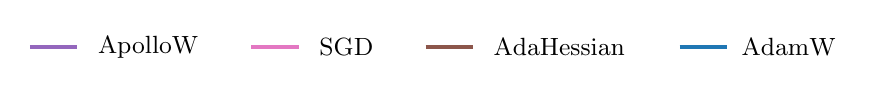
\begin{tikzpicture}[scale=0.75] % Nested TikZ environment
            \small 
            % AdaBelief
     \draw[mediumpurple148103189,  ultra thick] (0,0) -- ++(0.8,0);
     \node[anchor=west] at (1,0) {{ApolloW}}; % Increased spacing
     
     % Adam
    
     \draw[orchid227119194,  ultra thick] (3.75,0) -- ++(0.8,0);
     \node[anchor=west] at (4.75,0) {{SGD}}; % Increased spacing
     
     % AdaHessian
     \draw[sienna1408675,  ultra thick] (6.7,0) -- ++(0.8,0);
     \node[anchor=west] at (7.7,0) {{AdaHessian}}; % Increased spacing
     
     % Apollo
     \draw[steelblue31119180,  ultra thick] (11,0) -- ++(0.8,0);
     \node[anchor=west] at (11.9,0) {{AdamW}}; % Increased spacing
        
    \end{tikzpicture}
    };
    \end{tikzpicture}
     \\ 
    \end{tabular}
    \caption{Evaluation of optimizers on TinyImageNet using ResNet-18 with the \emph{milestone} learning rate scheduler, where hyperparameters
    where hyperparameters are choosen optimally across all optimizers. }
    \label{fig:tinyimagenet-perf-cosine}
\end{figure}
\begin{figure}[h!]
    \centering
    \begin{tabular}{cc}
        % This file was created with tikzplotlib v0.10.1.
\begin{tikzpicture}[scale=0.75]

    \definecolor{crimson2143940}{RGB}{214,39,40}
    \definecolor{darkgrey176}{RGB}{176,176,176}
    \definecolor{darkorange25512714}{RGB}{255,127,14}
    \definecolor{forestgreen4416044}{RGB}{44,160,44}
    \definecolor{grey127}{RGB}{127,127,127}
    \definecolor{lightgrey204}{RGB}{204,204,204}
    \definecolor{mediumpurple148103189}{RGB}{148,103,189}
    \definecolor{orchid227119194}{RGB}{227,119,194}
    \definecolor{sienna1408675}{RGB}{140,86,75}
    \definecolor{steelblue31119180}{RGB}{31,119,180}
    
    \begin{groupplot}[group style={group size=2 by 2,
        horizontal sep=1cm,  % Adjust horizontal spacing
        vertical sep=2cm}]
    \nextgroupplot[
    tick align=outside,
    tick pos=left,
    title={Polynom. Training Accuracy (milestone)},
    x grid style={darkgrey176},
    xlabel={Epochs},
    xmin=-5.95, xmax=124.95,
    xtick style={color=black},
    y grid style={darkgrey176},
    ymin=0.00580492726982097, ymax=1.04715423193734,
    ytick style={color=black}
    ]
    \addplot [semithick, steelblue31119180]
    table {%
    0 0.0919257512787724
    1 0.191384271099744
    2 0.252239849744246
    3 0.297668238491049
    4 0.334966432225064
    5 0.370796035805627
    6 0.401708359974425
    7 0.434498881074169
    8 0.46329523657289
    9 0.495196611253197
    10 0.527535565856777
    11 0.559658727621483
    12 0.591757912404092
    13 0.626508551790281
    14 0.663982576726343
    15 0.700681345907928
    16 0.732464833759591
    17 0.766981697570333
    18 0.794025735294118
    19 0.819375399616368
    20 0.839887707800511
    21 0.856507752557545
    22 0.871377477621483
    23 0.88359375
    24 0.894047714194373
    25 0.902099984015345
    26 0.9102961157289
    27 0.916905770460358
    28 0.918953804347826
    29 0.92582320971867
    30 0.931545716112532
    31 0.934522858056266
    32 0.936506953324808
    33 0.937829683503836
    34 0.942944773017903
    35 0.947200687340154
    36 0.950179827365729
    37 0.952779331841432
    38 0.955738491048593
    39 0.954591592071611
    40 0.95763067455243
    41 0.958555786445013
    42 0.962400095907928
    43 0.965706921355499
    44 0.966833839514066
    45 0.96701966112532
    46 0.968384351023018
    47 0.970893941815857
    48 0.97055027173913
    49 0.973705242966752
    50 0.97367527173913
    51 0.97490209398977
    52 0.976340712915601
    53 0.976810262148338
    54 0.979379795396419
    55 0.980047154731458
    56 0.980740489130435
    57 0.982504795396419
    58 0.983337995524297
    59 0.983867487212276
    60 0.984201166879795
    61 0.985721707161125
    62 0.987034446930946
    63 0.987923593350384
    64 0.988079443734015
    65 0.988373161764706
    66 0.988636908567775
    67 0.989410166240409
    68 0.991046595268542
    69 0.991598065856777
    70 0.991919757033248
    71 0.991885789641944
    72 0.992974744245524
    73 0.99303868286445
    74 0.994127637468031
    75 0.994185581841432
    76 0.994317455242967
    77 0.994583200127877
    78 0.995118686061381
    79 0.995236572890026
    80 0.996375479539642
    81 0.996213634910486
    82 0.996843030690537
    83 0.99690297314578
    84 0.997352541560102
    85 0.997532368925831
    86 0.997582320971867
    87 0.997912004475703
    88 0.997716192455243
    89 0.997786125319693
    90 0.998351582480818
    91 0.998331601662404
    92 0.998761189258312
    93 0.998721227621483
    94 0.998681265984655
    95 0.998631313938619
    96 0.998990968670077
    97 0.998951007033248
    98 0.998941016624041
    99 0.99898097826087
    100 0.999160805626598
    101 0.99919077685422
    102 0.99926070971867
    103 0.999290680946292
    104 0.999458519820972
    105 0.999340632992327
    106 0.99933064258312
    107 0.999320652173913
    108 0.999438539002558
    109 0.999490489130435
    110 0.999560421994885
    111 0.99947050831202
    112 0.999460517902813
    113 0.999444533248082
    114 0.999660326086957
    115 0.999518462276215
    116 0.999550431585678
    117 0.999500479539642
    118 0.999610374040921
    119 0.999630354859335
    };
    \addplot [semithick, darkorange25512714]
    table {%
    0 0.0898277653452685
    1 0.191326326726343
    2 0.245600223785166
    3 0.286051390664962
    4 0.319319453324808
    5 0.34712675831202
    6 0.373369565217391
    7 0.399678308823529
    8 0.420865968670077
    9 0.441681985294118
    10 0.464585997442455
    11 0.483983375959079
    12 0.504187979539642
    13 0.522298593350384
    14 0.546918957800511
    15 0.565982656649616
    16 0.585204203964194
    17 0.606839434143223
    18 0.624222746163683
    19 0.643158567774936
    20 0.662324168797954
    21 0.681140105498721
    22 0.701724344629156
    23 0.712208280051151
    24 0.729425751278772
    25 0.744397378516624
    26 0.755414801790281
    27 0.766344309462916
    28 0.783310022378517
    29 0.792085597826087
    30 0.800463554987212
    31 0.810637787723785
    32 0.81692175511509
    33 0.829076086956522
    34 0.832726582480818
    35 0.841717950767264
    36 0.846835038363171
    37 0.853063059462916
    38 0.858230099104859
    39 0.862184303069054
    40 0.868953804347826
    41 0.874912084398977
    42 0.87603300831202
    43 0.882704603580563
    44 0.884404971227621
    45 0.892417279411765
    46 0.894455322890025
    47 0.898711237212276
    48 0.902431665601023
    49 0.903576566496164
    50 0.908385949488491
    51 0.91418837915601
    52 0.913375159846547
    53 0.920184622762148
    54 0.920947890025575
    55 0.924020939897698
    56 0.925927109974425
    57 0.93072050831202
    58 0.934269101662404
    59 0.936373081841432
    60 0.937228260869565
    61 0.942639066496164
    62 0.94465712915601
    63 0.944757033248082
    64 0.951015025575448
    65 0.951424632352941
    66 0.952905210997442
    67 0.953622522378517
    68 0.959658727621483
    69 0.961237212276215
    70 0.963499040920716
    71 0.964390185421995
    72 0.966104539641944
    73 0.968396339514067
    74 0.97053628516624
    75 0.972128756393862
    76 0.973703244884911
    77 0.975193813938619
    78 0.976990089514067
    79 0.97943574168798
    80 0.979919277493606
    81 0.982043238491049
    82 0.982996323529412
    83 0.984614769820972
    84 0.986195252557545
    85 0.987579923273657
    86 0.989054507672634
    87 0.989711876598465
    88 0.99005354859335
    89 0.990293318414322
    90 0.991717950767263
    91 0.992615089514067
    92 0.993100623401534
    93 0.993100623401534
    94 0.993670076726343
    95 0.994810981457801
    96 0.995764066496164
    97 0.996327525575447
    98 0.996557304987212
    99 0.996753117007673
    100 0.997052829283887
    101 0.997436460997442
    102 0.997576326726343
    103 0.997840073529412
    104 0.997931985294118
    105 0.998265664961637
    106 0.998349584398977
    107 0.998565377237852
    108 0.998621323529412
    109 0.998761189258312
    110 0.998805147058824
    111 0.998731218030691
    112 0.998960997442455
    113 0.99906489769821
    114 0.999024936061381
    115 0.999010949488491
    116 0.999184782608696
    117 0.999340632992327
    118 0.999110853580563
    119 0.999094868925831
    };
    \addplot [semithick, forestgreen4416044]
    table {%
    0 0.0906869405370844
    1 0.190658967391304
    2 0.248831122122762
    3 0.298309622762148
    4 0.333335997442455
    5 0.368682065217391
    6 0.401222826086957
    7 0.43063658887468
    8 0.462124360613811
    9 0.495206601662404
    10 0.523315617007673
    11 0.558437899616368
    12 0.590325287723785
    13 0.627291799872123
    14 0.660202205882353
    15 0.699570412404092
    16 0.730872362531969
    17 0.763301230818414
    18 0.793302429667519
    19 0.816578085038363
    20 0.837691815856778
    21 0.856709558823529
    22 0.872226662404092
    23 0.882434862531969
    24 0.891681985294118
    25 0.902339753836317
    26 0.907564737851662
    27 0.915449168797954
    28 0.922604299872123
    29 0.927137947570333
    30 0.927737372122762
    31 0.932165121483376
    32 0.936135310102302
    33 0.937573929028133
    34 0.943500239769821
    35 0.945034766624041
    36 0.950143861892583
    37 0.952355738491049
    38 0.953238890664962
    39 0.955218989769821
    40 0.958925431585678
    41 0.95919317455243
    42 0.962390105498721
    43 0.963317215473146
    44 0.965215393222506
    45 0.967303388746803
    46 0.969956841432225
    47 0.969575207800512
    48 0.970436381074169
    49 0.971071771099744
    50 0.973657289002558
    51 0.975395620204604
    52 0.976728340792839
    53 0.979010150255754
    54 0.977675431585678
    55 0.978432704603581
    56 0.981160086317135
    57 0.982502797314578
    58 0.983262068414322
    59 0.984019341432225
    60 0.984520859974425
    61 0.985278132992327
    62 0.986726742327366
    63 0.986626838235294
    64 0.988201326726343
    65 0.988622921994885
    66 0.989154411764706
    67 0.990327285805627
    68 0.990093510230179
    69 0.991122522378517
    70 0.991941735933504
    71 0.992171515345268
    72 0.992547154731458
    73 0.992966751918159
    74 0.993899856138107
    75 0.993654092071611
    76 0.994145620204604
    77 0.994854939258312
    78 0.995056745524297
    79 0.995442375319693
    80 0.995778053069054
    81 0.995935901534527
    82 0.996101742327366
    83 0.996863011508951
    84 0.997232656649616
    85 0.997060821611253
    86 0.997426470588235
    87 0.997846067774936
    88 0.997662244245524
    89 0.99764226342711
    90 0.998015904731458
    91 0.998361572890026
    92 0.998571371483376
    93 0.998469469309463
    94 0.998435501918159
    95 0.998755195012788
    96 0.998791160485934
    97 0.998968989769821
    98 0.99898097826087
    99 0.999210757672634
    100 0.999300671355499
    101 0.998949008951407
    102 0.999090872762148
    103 0.999194773017903
    104 0.999380594629156
    105 0.999340632992327
    106 0.999340632992327
    107 0.999390585038363
    108 0.99940057544757
    109 0.999520460358056
    110 0.99934462915601
    111 0.999480498721228
    112 0.999640345268542
    113 0.999540441176471
    114 0.999510469948849
    115 0.999560421994885
    116 0.999540441176471
    117 0.999560421994885
    118 0.999620364450128
    119 0.999580402813299
    };
    \addplot [semithick, crimson2143940]
    table {%
    0 0.0558563778772379
    1 0.156513746803069
    2 0.230061141304348
    3 0.280870364450128
    4 0.31969908887468
    5 0.353582560741688
    6 0.381699568414322
    7 0.410991448209719
    8 0.436059382992327
    9 0.461351102941176
    10 0.483851502557545
    11 0.506108136189258
    12 0.530836397058823
    13 0.55295716112532
    14 0.573349584398977
    15 0.59538243286445
    16 0.615043558184143
    17 0.637176310741688
    18 0.659309063299233
    19 0.679162004475703
    20 0.699802189897698
    21 0.714869725063939
    22 0.735603820332481
    23 0.754791400255755
    24 0.766743925831202
    25 0.788107416879795
    26 0.796875
    27 0.814582001278772
    28 0.823453484654731
    29 0.838397138746803
    30 0.845150655370844
    31 0.853480658567775
    32 0.866496163682865
    33 0.871001838235294
    34 0.876356697570333
    35 0.886748721227621
    36 0.890509111253197
    37 0.895800031969309
    38 0.904461716751918
    39 0.909404971227622
    40 0.913982576726343
    41 0.917736972506394
    42 0.923049872122762
    43 0.926376678388747
    44 0.929000159846547
    45 0.934734654731458
    46 0.939134430946292
    47 0.941446211636829
    48 0.948071851023018
    49 0.951574488491049
    50 0.953604539641944
    51 0.955642583120205
    52 0.958100223785166
    53 0.962843670076726
    54 0.966961716751918
    55 0.968558184143223
    56 0.9709538842711
    57 0.972546355498721
    58 0.975327685421995
    59 0.978974184782609
    60 0.981839434143223
    61 0.983781569693095
    62 0.98772378516624
    63 0.988630914322251
    64 0.990127477621483
    65 0.992143542199489
    66 0.993813938618926
    67 0.994976822250639
    68 0.995128676470588
    69 0.996033807544757
    70 0.996837036445013
    71 0.997436460997442
    72 0.997921994884911
    73 0.998091831841432
    74 0.998391544117647
    75 0.998611333120205
    76 0.998945012787724
    77 0.999164801790281
    78 0.999094868925831
    79 0.999230738491049
    80 0.999284686700767
    81 0.999460517902813
    82 0.999440537084399
    83 0.99948449488491
    84 0.999420556265985
    85 0.999520460358056
    86 0.999590393222506
    87 0.999560421994885
    88 0.999660326086957
    89 0.999550431585678
    90 0.999610374040921
    91 0.999680306905371
    92 0.999594389386189
    93 0.999594389386189
    94 0.999580402813299
    95 0.999620364450128
    96 0.999660326086957
    97 0.999620364450128
    98 0.999630354859335
    99 0.999730258951407
    100 0.999680306905371
    101 0.999604379795396
    102 0.999760230179028
    103 0.9997202685422
    104 0.999670316496164
    105 0.999630354859335
    106 0.999670316496164
    107 0.999750239769821
    108 0.999810182225064
    109 0.999780210997442
    110 0.999760230179028
    111 0.999820172634271
    112 0.999730258951407
    113 0.999740249360614
    114 0.999760230179028
    115 0.999760230179028
    116 0.999770220588235
    117 0.999770220588235
    118 0.999740249360614
    119 0.999710278132992
    };
    \addplot [semithick, mediumpurple148103189]
    table {%
    0 0.056074168797954
    1 0.156541719948849
    2 0.228838315217391
    3 0.279539641943734
    4 0.3165461157289
    5 0.348551390664962
    6 0.380137068414322
    7 0.406004235933504
    8 0.431104140025575
    9 0.456541719948849
    10 0.479156010230179
    11 0.502909207161125
    12 0.524164801790281
    13 0.546061780690537
    14 0.564585997442455
    15 0.588676870204604
    16 0.61038003516624
    17 0.632462835677749
    18 0.652677429667519
    19 0.67247442455243
    20 0.692365329283887
    21 0.708987372122762
    22 0.726910166240409
    23 0.744439338235294
    24 0.762124360613811
    25 0.78035685741688
    26 0.788503037084399
    27 0.805744485294118
    28 0.811181265984655
    29 0.827967151534527
    30 0.841288363171356
    31 0.847378516624041
    32 0.85682145140665
    33 0.865473145780051
    34 0.873405530690537
    35 0.880187020460358
    36 0.885861572890026
    37 0.893500239769821
    38 0.897993925831202
    39 0.904078085038363
    40 0.905994245524297
    41 0.912392103580563
    42 0.916783887468031
    43 0.920937899616368
    44 0.927135949488491
    45 0.930938299232737
    46 0.934299072890026
    47 0.935583839514066
    48 0.939607976342711
    49 0.943442295396419
    50 0.948357576726343
    51 0.954355818414322
    52 0.956523737212276
    53 0.961429028132992
    54 0.965253356777494
    55 0.966869804987212
    56 0.970804028132992
    57 0.973007912404092
    58 0.97568334398977
    59 0.978784367007673
    60 0.980208999360614
    61 0.984578804347826
    62 0.986752717391304
    63 0.989875719309463
    64 0.991681985294118
    65 0.992830882352941
    66 0.993630115089514
    67 0.995554267902813
    68 0.996727141943734
    69 0.99676310741688
    70 0.997300591432225
    71 0.998069852941176
    72 0.998375559462916
    73 0.998291640025575
    74 0.998831122122762
    75 0.998951007033248
    76 0.999100863171355
    77 0.999158807544757
    78 0.999310661764706
    79 0.999530450767263
    80 0.999500479539642
    81 0.99941456202046
    82 0.999460517902813
    83 0.999524456521739
    84 0.999550431585678
    85 0.999630354859335
    86 0.999580402813299
    87 0.999540441176471
    88 0.999630354859335
    89 0.999620364450128
    90 0.999590393222506
    91 0.999670316496164
    92 0.999640345268542
    93 0.999704283887468
    94 0.999600383631714
    95 0.999640345268542
    96 0.9997202685422
    97 0.999588395140665
    98 0.999700287723785
    99 0.999740249360614
    100 0.999700287723785
    101 0.999730258951407
    102 0.999760230179028
    103 0.999620364450128
    104 0.999710278132992
    105 0.999700287723785
    106 0.999740249360614
    107 0.9997202685422
    108 0.999780210997442
    109 0.999730258951407
    110 0.9997202685422
    111 0.999750239769821
    112 0.999710278132992
    113 0.999664322250639
    114 0.999800191815857
    115 0.99979020140665
    116 0.999740249360614
    117 0.999820172634271
    118 0.99979020140665
    119 0.99979020140665
    };
    \addplot [semithick, sienna1408675]
    table {%
    0 0.0583240089514067
    1 0.154315856777494
    2 0.22248841112532
    3 0.2681086157289
    4 0.302521579283887
    5 0.331315936700767
    6 0.357740569053708
    7 0.383096227621483
    8 0.403480658567775
    9 0.421809063299233
    10 0.437356138107417
    11 0.454140025575448
    12 0.469950847186701
    13 0.481697570332481
    14 0.494029731457801
    15 0.507408887468031
    16 0.521249600383632
    17 0.531373881074169
    18 0.543060661764706
    19 0.553119005754476
    20 0.562270220588235
    21 0.576118925831202
    22 0.583655690537084
    23 0.598547394501279
    24 0.610048353580563
    25 0.625679347826087
    26 0.636916560102302
    27 0.649868126598465
    28 0.666256393861893
    29 0.67727381713555
    30 0.688610933503836
    31 0.705374840153453
    32 0.718204523657289
    33 0.732217071611253
    34 0.74440537084399
    35 0.755514705882353
    36 0.769359414961637
    37 0.780262947570332
    38 0.793328404731458
    39 0.801454603580563
    40 0.81399256713555
    41 0.825051950127877
    42 0.834185182225064
    43 0.841729939258312
    44 0.850943094629156
    45 0.854209958439898
    46 0.866899776214834
    47 0.874062899616368
    48 0.882674632352941
    49 0.889897698209719
    50 0.892643062659846
    51 0.897923992966752
    52 0.905065137468031
    53 0.909426950127877
    54 0.916903772378517
    55 0.921759111253197
    56 0.93141783887468
    57 0.934410965473146
    58 0.939597985933504
    59 0.942279411764706
    60 0.945324488491049
    61 0.949220748081841
    62 0.953732416879795
    63 0.95786844629156
    64 0.959860533887468
    65 0.965898737212276
    66 0.966785885549872
    67 0.969928868286445
    68 0.973901054987212
    69 0.97668837915601
    70 0.976872202685422
    71 0.979919277493606
    72 0.983553788363171
    73 0.984740648976982
    74 0.985320092710998
    75 0.987777733375959
    76 0.988209319053708
    77 0.990419197570332
    78 0.991190457161125
    79 0.99278692455243
    80 0.993264466112532
    81 0.995358455882353
    82 0.995316496163683
    83 0.995736093350384
    84 0.995927909207161
    85 0.996773097826087
    86 0.997634271099744
    87 0.997626278772378
    88 0.997973945012788
    89 0.998461476982097
    90 0.998415521099744
    91 0.998621323529412
    92 0.998709239130435
    93 0.998589354219949
    94 0.998801150895141
    95 0.998875079923274
    96 0.999060901534527
    97 0.999164801790281
    98 0.99940057544757
    99 0.999350623401535
    100 0.999480498721228
    101 0.999530450767263
    102 0.999480498721228
    103 0.999450527493606
    104 0.999580402813299
    105 0.99947050831202
    106 0.999570412404092
    107 0.999490489130435
    108 0.999630354859335
    109 0.999620364450128
    110 0.999620364450128
    111 0.999624360613811
    112 0.999700287723785
    113 0.999630354859335
    114 0.999630354859335
    115 0.999750239769821
    116 0.9997202685422
    117 0.999680306905371
    118 0.999680306905371
    119 0.999690297314578
    };
    \addplot [semithick, orchid227119194]
    table {%
    0 0.0534127237851662
    1 0.135809622762148
    2 0.194093670076726
    3 0.233505834398977
    4 0.267319373401534
    5 0.294691096547315
    6 0.321047794117647
    7 0.344309462915601
    8 0.367495204603581
    9 0.389170396419437
    10 0.410815617007673
    11 0.43108216112532
    12 0.452411684782609
    13 0.476686381074169
    14 0.495498321611253
    15 0.519749040920716
    16 0.541548113810742
    17 0.560893542199489
    18 0.580766464194373
    19 0.602052030051151
    20 0.629297874040921
    21 0.647714194373401
    22 0.672620284526854
    23 0.694193574168798
    24 0.716066576086956
    25 0.736093350383632
    26 0.754485693734015
    27 0.7759211157289
    28 0.792774936061381
    29 0.816012627877238
    30 0.829303868286445
    31 0.84835358056266
    32 0.864558024296675
    33 0.875317695012788
    34 0.890207400895141
    35 0.900059942455243
    36 0.91117527173913
    37 0.918979779411765
    38 0.92806905370844
    39 0.934726662404092
    40 0.943398337595908
    41 0.946892982736573
    42 0.951342710997442
    43 0.958919437340154
    44 0.962623881074169
    45 0.96628037084399
    46 0.969571211636829
    47 0.972904012148338
    48 0.975459558823529
    49 0.977529571611253
    50 0.980155051150895
    51 0.982418877877238
    52 0.984422953964194
    53 0.986241208439898
    54 0.988437100383632
    55 0.98876878196931
    56 0.989795796035806
    57 0.991152493606138
    58 0.991194453324808
    59 0.992459239130435
    60 0.993004715473146
    61 0.993542199488491
    62 0.994373401534527
    63 0.994463315217391
    64 0.995708120204604
    65 0.995232576726343
    66 0.995702125959079
    67 0.996267583120205
    68 0.996563299232737
    69 0.996807065217391
    70 0.997282608695652
    71 0.997272618286445
    72 0.997452445652174
    73 0.997576326726343
    74 0.997896019820972
    75 0.997975943094629
    76 0.998259670716113
    77 0.998101822250639
    78 0.998411524936061
    79 0.998425511508951
    80 0.998421515345269
    81 0.99832560741688
    82 0.998735214194373
    83 0.998519421355499
    84 0.998705242966752
    85 0.998541400255754
    86 0.998990968670077
    87 0.998669277493606
    88 0.998970987851662
    89 0.998945012787724
    90 0.998755195012788
    91 0.998994964833759
    92 0.999150815217391
    93 0.99905091112532
    94 0.999080882352941
    95 0.999038922634271
    96 0.999110853580563
    97 0.999160805626598
    98 0.998955003196931
    99 0.999030930306905
    100 0.999020939897698
    101 0.999070891943734
    102 0.999180786445013
    103 0.999350623401535
    104 0.99919077685422
    105 0.999320652173913
    106 0.99926070971867
    107 0.99940057544757
    108 0.999128836317136
    109 0.999180786445013
    110 0.999280690537084
    111 0.999364609974424
    112 0.99940057544757
    113 0.999244725063939
    114 0.999410565856777
    115 0.99933064258312
    116 0.999200767263427
    117 0.999224744245524
    118 0.999290680946292
    119 0.999340632992327
    };
    \addplot [semithick, grey127]
    table {%
    0 0.05313898657289
    1 0.145935901534527
    2 0.209746643222506
    3 0.259642742966752
    4 0.298751198849105
    5 0.334484894501279
    6 0.367331361892583
    7 0.398277653452685
    8 0.428422714194373
    9 0.457352941176471
    10 0.490055546675192
    11 0.524178788363171
    12 0.555882352941176
    13 0.591282368925831
    14 0.62910206202046
    15 0.662743765984655
    16 0.696003836317135
    17 0.726870204603581
    18 0.758929427749361
    19 0.786255195012788
    20 0.80910925511509
    21 0.830848385549872
    22 0.845696131713555
    23 0.862008471867008
    24 0.877054028132992
    25 0.884369005754476
    26 0.893793957800512
    27 0.90216192455243
    28 0.910633791560102
    29 0.916711956521739
    30 0.921287563938619
    31 0.925217790920716
    32 0.931865409207161
    33 0.935262148337596
    34 0.938035485933504
    35 0.941500159846547
    36 0.944399376598466
    37 0.948523417519182
    38 0.951042998721228
    39 0.9534047314578
    40 0.956114130434783
    41 0.957934382992327
    42 0.96243006713555
    43 0.96223425511509
    44 0.964965632992327
    45 0.965539082480818
    46 0.968076646419437
    47 0.969789002557545
    48 0.971713155370844
    49 0.973017902813299
    50 0.973539402173913
    51 0.97476222826087
    52 0.97657648657289
    53 0.977577525575448
    54 0.977409686700767
    55 0.980890345268542
    56 0.980570652173913
    57 0.981897378516624
    58 0.98285445971867
    59 0.983931425831202
    60 0.98494645140665
    61 0.985785645780051
    62 0.987012468030691
    63 0.986744725063939
    64 0.987715792838875
    65 0.988732816496164
    66 0.988902653452685
    67 0.98982976342711
    68 0.990780850383632
    69 0.991552109974424
    70 0.991218430306905
    71 0.992409287084399
    72 0.993000719309463
    73 0.992705003196931
    74 0.993877877237852
    75 0.99397378516624
    76 0.994319453324808
    77 0.994717071611253
    78 0.994902893222506
    79 0.995502317774936
    80 0.995568254475703
    81 0.996377477621483
    82 0.99616368286445
    83 0.996641224424552
    84 0.996942934782609
    85 0.997082800511509
    86 0.997106777493606
    87 0.997372522378517
    88 0.997616288363171
    89 0.998091831841432
    90 0.997975943094629
    91 0.998481457800512
    92 0.998495444373401
    93 0.998551390664962
    94 0.998631313938619
    95 0.998781170076726
    96 0.998835118286445
    97 0.998765185421995
    98 0.998901054987212
    99 0.999014945652174
    100 0.998970987851662
    101 0.999140824808184
    102 0.99913483056266
    103 0.999314657928389
    104 0.99919077685422
    105 0.99920476342711
    106 0.999450527493606
    107 0.99941456202046
    108 0.99933064258312
    109 0.999390585038363
    110 0.999570412404092
    111 0.999510469948849
    112 0.999520460358056
    113 0.999590393222506
    114 0.999510469948849
    115 0.999540441176471
    116 0.999508471867008
    117 0.999570412404092
    118 0.99948449488491
    119 0.999580402813299
    };
    
    \nextgroupplot[
    tick align=outside,
    tick pos=left,
    title={Polynom. Test Accuracy (milestone)},
    x grid style={darkgrey176},
    xlabel={Epochs},
    xmin=-5.95, xmax=124.95,
    xtick style={color=black},
    y grid style={darkgrey176},
    ymin=0.07869140625, ymax=0.46154296875,
    ytick style={color=black}
    ]
    \addplot [semithick, steelblue31119180]
    table {%
    0 0.141015625
    1 0.20078125
    2 0.25673828125
    3 0.2904296875
    4 0.33212890625
    5 0.33486328125
    6 0.36474609375
    7 0.3783203125
    8 0.38359375
    9 0.38466796875
    10 0.39638671875
    11 0.3951171875
    12 0.39814453125
    13 0.40732421875
    14 0.39951171875
    15 0.40390625
    16 0.38759765625
    17 0.39365234375
    18 0.3908203125
    19 0.3859375
    20 0.38798828125
    21 0.39541015625
    22 0.39208984375
    23 0.3865234375
    24 0.38935546875
    25 0.386328125
    26 0.3828125
    27 0.3830078125
    28 0.387109375
    29 0.3923828125
    30 0.3806640625
    31 0.37939453125
    32 0.38671875
    33 0.38779296875
    34 0.38486328125
    35 0.38837890625
    36 0.39287109375
    37 0.38720703125
    38 0.39072265625
    39 0.3880859375
    40 0.387109375
    41 0.387109375
    42 0.38681640625
    43 0.38837890625
    44 0.38408203125
    45 0.3861328125
    46 0.39443359375
    47 0.39130859375
    48 0.390234375
    49 0.385546875
    50 0.3912109375
    51 0.38388671875
    52 0.3884765625
    53 0.3912109375
    54 0.38955078125
    55 0.3884765625
    56 0.39873046875
    57 0.39208984375
    58 0.39345703125
    59 0.39658203125
    60 0.39443359375
    61 0.39501953125
    62 0.3953125
    63 0.39599609375
    64 0.396484375
    65 0.395703125
    66 0.3953125
    67 0.391015625
    68 0.39658203125
    69 0.400390625
    70 0.39384765625
    71 0.39951171875
    72 0.4015625
    73 0.39755859375
    74 0.3970703125
    75 0.39697265625
    76 0.396484375
    77 0.40498046875
    78 0.39736328125
    79 0.4009765625
    80 0.4005859375
    81 0.4037109375
    82 0.40078125
    83 0.40546875
    84 0.40615234375
    85 0.4080078125
    86 0.4056640625
    87 0.40888671875
    88 0.408203125
    89 0.4083984375
    90 0.4078125
    91 0.41181640625
    92 0.4091796875
    93 0.409375
    94 0.40673828125
    95 0.40625
    96 0.40712890625
    97 0.4109375
    98 0.40927734375
    99 0.40888671875
    100 0.41005859375
    101 0.40947265625
    102 0.41201171875
    103 0.4142578125
    104 0.41123046875
    105 0.413671875
    106 0.4130859375
    107 0.4150390625
    108 0.41376953125
    109 0.4140625
    110 0.41455078125
    111 0.416015625
    112 0.4150390625
    113 0.41630859375
    114 0.41318359375
    115 0.415234375
    116 0.4162109375
    117 0.41767578125
    118 0.41689453125
    119 0.41708984375
    };
    \addplot [semithick, darkorange25512714]
    table {%
    0 0.14130859375
    1 0.218359375
    2 0.2666015625
    3 0.291015625
    4 0.3
    5 0.30986328125
    6 0.346875
    7 0.3556640625
    8 0.36396484375
    9 0.36025390625
    10 0.39677734375
    11 0.40009765625
    12 0.3982421875
    13 0.39736328125
    14 0.4115234375
    15 0.4126953125
    16 0.41728515625
    17 0.41416015625
    18 0.41455078125
    19 0.4041015625
    20 0.39443359375
    21 0.41416015625
    22 0.4001953125
    23 0.40673828125
    24 0.40517578125
    25 0.3958984375
    26 0.402734375
    27 0.40869140625
    28 0.39462890625
    29 0.40029296875
    30 0.39716796875
    31 0.3986328125
    32 0.3939453125
    33 0.4044921875
    34 0.39765625
    35 0.39912109375
    36 0.39775390625
    37 0.3962890625
    38 0.403125
    39 0.3916015625
    40 0.39150390625
    41 0.40234375
    42 0.4048828125
    43 0.4
    44 0.3970703125
    45 0.4009765625
    46 0.39814453125
    47 0.40048828125
    48 0.401171875
    49 0.39873046875
    50 0.39912109375
    51 0.3955078125
    52 0.399609375
    53 0.39619140625
    54 0.39365234375
    55 0.39951171875
    56 0.404296875
    57 0.405859375
    58 0.40625
    59 0.40595703125
    60 0.39853515625
    61 0.40927734375
    62 0.401171875
    63 0.39921875
    64 0.40419921875
    65 0.40517578125
    66 0.403125
    67 0.4056640625
    68 0.40576171875
    69 0.40712890625
    70 0.409765625
    71 0.40537109375
    72 0.40517578125
    73 0.41279296875
    74 0.41513671875
    75 0.4109375
    76 0.409375
    77 0.41396484375
    78 0.41513671875
    79 0.41259765625
    80 0.41455078125
    81 0.4171875
    82 0.419921875
    83 0.41904296875
    84 0.4185546875
    85 0.41748046875
    86 0.4203125
    87 0.41943359375
    88 0.41552734375
    89 0.4173828125
    90 0.42314453125
    91 0.42431640625
    92 0.428515625
    93 0.41953125
    94 0.4265625
    95 0.42314453125
    96 0.4265625
    97 0.4263671875
    98 0.42919921875
    99 0.42529296875
    100 0.4279296875
    101 0.4271484375
    102 0.425390625
    103 0.42890625
    104 0.43408203125
    105 0.43125
    106 0.4314453125
    107 0.43427734375
    108 0.43486328125
    109 0.4333984375
    110 0.4330078125
    111 0.4330078125
    112 0.4310546875
    113 0.43427734375
    114 0.43447265625
    115 0.43251953125
    116 0.4318359375
    117 0.4328125
    118 0.4328125
    119 0.434375
    };
    \addplot [semithick, forestgreen4416044]
    table {%
    0 0.16103515625
    1 0.22880859375
    2 0.2634765625
    3 0.3
    4 0.3326171875
    5 0.33505859375
    6 0.3470703125
    7 0.37392578125
    8 0.38671875
    9 0.38896484375
    10 0.39599609375
    11 0.3974609375
    12 0.4048828125
    13 0.3865234375
    14 0.4095703125
    15 0.39638671875
    16 0.408984375
    17 0.39677734375
    18 0.40341796875
    19 0.3916015625
    20 0.38232421875
    21 0.391796875
    22 0.39384765625
    23 0.3947265625
    24 0.38427734375
    25 0.3849609375
    26 0.38486328125
    27 0.3802734375
    28 0.3814453125
    29 0.39140625
    30 0.3822265625
    31 0.385546875
    32 0.39228515625
    33 0.38642578125
    34 0.3888671875
    35 0.383984375
    36 0.3935546875
    37 0.38525390625
    38 0.39169921875
    39 0.3876953125
    40 0.3896484375
    41 0.3890625
    42 0.39541015625
    43 0.3861328125
    44 0.3921875
    45 0.39013671875
    46 0.3880859375
    47 0.3939453125
    48 0.38798828125
    49 0.3916015625
    50 0.39345703125
    51 0.388671875
    52 0.3888671875
    53 0.39248046875
    54 0.38896484375
    55 0.39130859375
    56 0.39462890625
    57 0.3978515625
    58 0.399609375
    59 0.3955078125
    60 0.39482421875
    61 0.3951171875
    62 0.395703125
    63 0.39921875
    64 0.3982421875
    65 0.40283203125
    66 0.40478515625
    67 0.40146484375
    68 0.401953125
    69 0.40283203125
    70 0.40283203125
    71 0.40634765625
    72 0.40185546875
    73 0.40048828125
    74 0.4001953125
    75 0.40634765625
    76 0.4037109375
    77 0.40703125
    78 0.40537109375
    79 0.40458984375
    80 0.40703125
    81 0.40791015625
    82 0.4078125
    83 0.41005859375
    84 0.4072265625
    85 0.40771484375
    86 0.410546875
    87 0.40869140625
    88 0.41083984375
    89 0.40673828125
    90 0.41123046875
    91 0.41494140625
    92 0.41416015625
    93 0.4130859375
    94 0.4109375
    95 0.4134765625
    96 0.4125
    97 0.414453125
    98 0.41376953125
    99 0.4134765625
    100 0.413671875
    101 0.41357421875
    102 0.4123046875
    103 0.41650390625
    104 0.41494140625
    105 0.413671875
    106 0.41689453125
    107 0.41591796875
    108 0.4146484375
    109 0.4169921875
    110 0.41669921875
    111 0.41884765625
    112 0.4193359375
    113 0.41845703125
    114 0.41865234375
    115 0.419140625
    116 0.41923828125
    117 0.41923828125
    118 0.4162109375
    119 0.4171875
    };
    \addplot [semithick, crimson2143940]
    table {%
    0 0.1076171875
    1 0.19931640625
    2 0.23720703125
    3 0.28486328125
    4 0.30888671875
    5 0.3373046875
    6 0.35126953125
    7 0.347265625
    8 0.3708984375
    9 0.3771484375
    10 0.3810546875
    11 0.3830078125
    12 0.376953125
    13 0.37666015625
    14 0.3859375
    15 0.38564453125
    16 0.3890625
    17 0.38798828125
    18 0.380078125
    19 0.39716796875
    20 0.387109375
    21 0.38310546875
    22 0.38310546875
    23 0.38017578125
    24 0.38251953125
    25 0.37578125
    26 0.38935546875
    27 0.390625
    28 0.3859375
    29 0.39013671875
    30 0.385546875
    31 0.3923828125
    32 0.3833984375
    33 0.38603515625
    34 0.3896484375
    35 0.3853515625
    36 0.3822265625
    37 0.38525390625
    38 0.3837890625
    39 0.38525390625
    40 0.39091796875
    41 0.38671875
    42 0.38740234375
    43 0.3900390625
    44 0.39404296875
    45 0.3884765625
    46 0.38759765625
    47 0.3884765625
    48 0.3896484375
    49 0.3935546875
    50 0.39775390625
    51 0.39765625
    52 0.3935546875
    53 0.3986328125
    54 0.3998046875
    55 0.40185546875
    56 0.4005859375
    57 0.40234375
    58 0.3984375
    59 0.4033203125
    60 0.40556640625
    61 0.4068359375
    62 0.40703125
    63 0.4119140625
    64 0.41640625
    65 0.41748046875
    66 0.41787109375
    67 0.41640625
    68 0.42158203125
    69 0.41826171875
    70 0.4251953125
    71 0.4236328125
    72 0.4302734375
    73 0.4361328125
    74 0.4283203125
    75 0.4330078125
    76 0.43115234375
    77 0.432421875
    78 0.4330078125
    79 0.4369140625
    80 0.43310546875
    81 0.43837890625
    82 0.4373046875
    83 0.4357421875
    84 0.43837890625
    85 0.43671875
    86 0.43857421875
    87 0.4357421875
    88 0.4375
    89 0.43642578125
    90 0.43857421875
    91 0.44013671875
    92 0.4380859375
    93 0.43779296875
    94 0.43642578125
    95 0.4396484375
    96 0.44208984375
    97 0.44033203125
    98 0.4392578125
    99 0.44140625
    100 0.441015625
    101 0.44111328125
    102 0.4412109375
    103 0.441015625
    104 0.44111328125
    105 0.440625
    106 0.4388671875
    107 0.44189453125
    108 0.4423828125
    109 0.440234375
    110 0.4404296875
    111 0.44091796875
    112 0.442578125
    113 0.44013671875
    114 0.43994140625
    115 0.44169921875
    116 0.4396484375
    117 0.44013671875
    118 0.438671875
    119 0.4431640625
    };
    \addplot [semithick, mediumpurple148103189]
    table {%
    0 0.09697265625
    1 0.20166015625
    2 0.2650390625
    3 0.28583984375
    4 0.2873046875
    5 0.32998046875
    6 0.33154296875
    7 0.34853515625
    8 0.34794921875
    9 0.36806640625
    10 0.36845703125
    11 0.365625
    12 0.373828125
    13 0.38330078125
    14 0.38193359375
    15 0.3958984375
    16 0.38349609375
    17 0.39453125
    18 0.38662109375
    19 0.37841796875
    20 0.3921875
    21 0.37802734375
    22 0.3826171875
    23 0.37685546875
    24 0.37578125
    25 0.383984375
    26 0.38125
    27 0.36337890625
    28 0.37783203125
    29 0.383203125
    30 0.37685546875
    31 0.3720703125
    32 0.379296875
    33 0.38505859375
    34 0.35029296875
    35 0.38095703125
    36 0.383984375
    37 0.38681640625
    38 0.3751953125
    39 0.388671875
    40 0.38076171875
    41 0.37880859375
    42 0.37763671875
    43 0.38857421875
    44 0.3837890625
    45 0.39375
    46 0.38955078125
    47 0.38603515625
    48 0.390234375
    49 0.38837890625
    50 0.38779296875
    51 0.39169921875
    52 0.3923828125
    53 0.3888671875
    54 0.39658203125
    55 0.39638671875
    56 0.39541015625
    57 0.39931640625
    58 0.3984375
    59 0.40361328125
    60 0.404296875
    61 0.401171875
    62 0.40380859375
    63 0.40888671875
    64 0.40927734375
    65 0.41357421875
    66 0.4140625
    67 0.42109375
    68 0.41708984375
    69 0.417578125
    70 0.42109375
    71 0.42080078125
    72 0.42724609375
    73 0.427734375
    74 0.429296875
    75 0.4333984375
    76 0.4318359375
    77 0.42939453125
    78 0.43447265625
    79 0.43544921875
    80 0.4333984375
    81 0.43466796875
    82 0.4349609375
    83 0.4353515625
    84 0.43388671875
    85 0.4333984375
    86 0.437109375
    87 0.4388671875
    88 0.4384765625
    89 0.4400390625
    90 0.43828125
    91 0.4392578125
    92 0.43564453125
    93 0.43828125
    94 0.4416015625
    95 0.441015625
    96 0.440625
    97 0.4373046875
    98 0.43876953125
    99 0.44228515625
    100 0.44130859375
    101 0.4421875
    102 0.44189453125
    103 0.44189453125
    104 0.444140625
    105 0.4419921875
    106 0.4408203125
    107 0.4435546875
    108 0.4404296875
    109 0.436328125
    110 0.4416015625
    111 0.44091796875
    112 0.4412109375
    113 0.4423828125
    114 0.4412109375
    115 0.4423828125
    116 0.4435546875
    117 0.44150390625
    118 0.4416015625
    119 0.43955078125
    };
    \addplot [semithick, sienna1408675]
    table {%
    0 0.10234375
    1 0.1759765625
    2 0.24052734375
    3 0.2744140625
    4 0.2888671875
    5 0.30615234375
    6 0.31328125
    7 0.3376953125
    8 0.33583984375
    9 0.36162109375
    10 0.36005859375
    11 0.378125
    12 0.35458984375
    13 0.37080078125
    14 0.36796875
    15 0.36171875
    16 0.3759765625
    17 0.37705078125
    18 0.36630859375
    19 0.37109375
    20 0.3703125
    21 0.38095703125
    22 0.36767578125
    23 0.365234375
    24 0.368359375
    25 0.3736328125
    26 0.37060546875
    27 0.35966796875
    28 0.34677734375
    29 0.38427734375
    30 0.37568359375
    31 0.37724609375
    32 0.37578125
    33 0.3544921875
    34 0.3734375
    35 0.37548828125
    36 0.3630859375
    37 0.36396484375
    38 0.36923828125
    39 0.36796875
    40 0.3830078125
    41 0.37060546875
    42 0.35126953125
    43 0.37001953125
    44 0.36884765625
    45 0.35888671875
    46 0.373046875
    47 0.36279296875
    48 0.37021484375
    49 0.37451171875
    50 0.3755859375
    51 0.38203125
    52 0.37392578125
    53 0.3783203125
    54 0.37548828125
    55 0.39404296875
    56 0.3861328125
    57 0.3890625
    58 0.38955078125
    59 0.38076171875
    60 0.39423828125
    61 0.39296875
    62 0.39501953125
    63 0.40009765625
    64 0.39560546875
    65 0.4
    66 0.39140625
    67 0.39609375
    68 0.39033203125
    69 0.4109375
    70 0.4033203125
    71 0.3990234375
    72 0.40751953125
    73 0.40712890625
    74 0.41337890625
    75 0.4166015625
    76 0.409375
    77 0.411328125
    78 0.4173828125
    79 0.41884765625
    80 0.41767578125
    81 0.41630859375
    82 0.42099609375
    83 0.421484375
    84 0.41279296875
    85 0.42119140625
    86 0.43212890625
    87 0.426953125
    88 0.4251953125
    89 0.42861328125
    90 0.42568359375
    91 0.430078125
    92 0.43125
    93 0.42470703125
    94 0.4302734375
    95 0.43173828125
    96 0.43046875
    97 0.43154296875
    98 0.43583984375
    99 0.43525390625
    100 0.437109375
    101 0.43974609375
    102 0.43583984375
    103 0.43798828125
    104 0.4396484375
    105 0.440234375
    106 0.43740234375
    107 0.44130859375
    108 0.442578125
    109 0.43828125
    110 0.44091796875
    111 0.4392578125
    112 0.4404296875
    113 0.43994140625
    114 0.43955078125
    115 0.44091796875
    116 0.44013671875
    117 0.4416015625
    118 0.4431640625
    119 0.4408203125
    };
    \addplot [semithick, orchid227119194]
    table {%
    0 0.10341796875
    1 0.16484375
    2 0.2078125
    3 0.23759765625
    4 0.2595703125
    5 0.2669921875
    6 0.304296875
    7 0.31044921875
    8 0.321484375
    9 0.341796875
    10 0.32978515625
    11 0.3388671875
    12 0.34970703125
    13 0.339453125
    14 0.33896484375
    15 0.3564453125
    16 0.363671875
    17 0.3568359375
    18 0.3611328125
    19 0.35693359375
    20 0.3615234375
    21 0.36181640625
    22 0.36748046875
    23 0.3564453125
    24 0.35732421875
    25 0.36357421875
    26 0.36533203125
    27 0.35947265625
    28 0.36005859375
    29 0.3560546875
    30 0.3623046875
    31 0.35830078125
    32 0.36083984375
    33 0.3607421875
    34 0.36435546875
    35 0.36064453125
    36 0.36162109375
    37 0.36591796875
    38 0.3673828125
    39 0.362890625
    40 0.36015625
    41 0.36416015625
    42 0.37001953125
    43 0.3650390625
    44 0.36982421875
    45 0.3658203125
    46 0.36474609375
    47 0.36904296875
    48 0.368359375
    49 0.36640625
    50 0.3677734375
    51 0.37001953125
    52 0.37119140625
    53 0.37958984375
    54 0.37177734375
    55 0.3689453125
    56 0.37529296875
    57 0.3771484375
    58 0.37265625
    59 0.3787109375
    60 0.37744140625
    61 0.3765625
    62 0.3765625
    63 0.37685546875
    64 0.37666015625
    65 0.381640625
    66 0.37861328125
    67 0.3826171875
    68 0.3822265625
    69 0.37919921875
    70 0.37802734375
    71 0.38251953125
    72 0.38271484375
    73 0.38291015625
    74 0.37919921875
    75 0.38349609375
    76 0.38134765625
    77 0.3828125
    78 0.38046875
    79 0.38251953125
    80 0.38310546875
    81 0.3849609375
    82 0.3861328125
    83 0.38623046875
    84 0.38603515625
    85 0.38896484375
    86 0.38681640625
    87 0.3859375
    88 0.3869140625
    89 0.3884765625
    90 0.38662109375
    91 0.38369140625
    92 0.38671875
    93 0.38642578125
    94 0.3873046875
    95 0.387890625
    96 0.3884765625
    97 0.3875
    98 0.386328125
    99 0.385546875
    100 0.38642578125
    101 0.38837890625
    102 0.3876953125
    103 0.3873046875
    104 0.3888671875
    105 0.38623046875
    106 0.38955078125
    107 0.38720703125
    108 0.3888671875
    109 0.3892578125
    110 0.38740234375
    111 0.38701171875
    112 0.388671875
    113 0.3869140625
    114 0.3880859375
    115 0.38857421875
    116 0.3884765625
    117 0.3873046875
    118 0.3875
    119 0.38564453125
    };
    \addplot [semithick, grey127]
    table {%
    0 0.09609375
    1 0.1751953125
    2 0.233203125
    3 0.17373046875
    4 0.24384765625
    5 0.300390625
    6 0.29873046875
    7 0.26904296875
    8 0.31865234375
    9 0.340625
    10 0.31748046875
    11 0.3638671875
    12 0.3701171875
    13 0.35771484375
    14 0.35341796875
    15 0.35751953125
    16 0.366015625
    17 0.35263671875
    18 0.3572265625
    19 0.34697265625
    20 0.3623046875
    21 0.36240234375
    22 0.34873046875
    23 0.350390625
    24 0.3537109375
    25 0.359765625
    26 0.3455078125
    27 0.347265625
    28 0.3666015625
    29 0.3546875
    30 0.3544921875
    31 0.35458984375
    32 0.3447265625
    33 0.35576171875
    34 0.35625
    35 0.36201171875
    36 0.359375
    37 0.368359375
    38 0.37119140625
    39 0.36064453125
    40 0.36513671875
    41 0.35927734375
    42 0.3671875
    43 0.3392578125
    44 0.37060546875
    45 0.3662109375
    46 0.3599609375
    47 0.3705078125
    48 0.37158203125
    49 0.3630859375
    50 0.36044921875
    51 0.37109375
    52 0.3693359375
    53 0.369140625
    54 0.37294921875
    55 0.37021484375
    56 0.37373046875
    57 0.3734375
    58 0.3744140625
    59 0.373828125
    60 0.3736328125
    61 0.37763671875
    62 0.37705078125
    63 0.36826171875
    64 0.37314453125
    65 0.37705078125
    66 0.3791015625
    67 0.37451171875
    68 0.37373046875
    69 0.37666015625
    70 0.37919921875
    71 0.37802734375
    72 0.38310546875
    73 0.382421875
    74 0.37861328125
    75 0.37314453125
    76 0.3837890625
    77 0.3849609375
    78 0.38701171875
    79 0.3826171875
    80 0.37890625
    81 0.38623046875
    82 0.3814453125
    83 0.38466796875
    84 0.391015625
    85 0.38544921875
    86 0.38623046875
    87 0.38671875
    88 0.3853515625
    89 0.38984375
    90 0.38583984375
    91 0.39033203125
    92 0.39169921875
    93 0.39296875
    94 0.39326171875
    95 0.3958984375
    96 0.39453125
    97 0.39384765625
    98 0.39443359375
    99 0.39287109375
    100 0.3951171875
    101 0.39697265625
    102 0.39697265625
    103 0.3962890625
    104 0.3935546875
    105 0.394140625
    106 0.39462890625
    107 0.39423828125
    108 0.395703125
    109 0.39423828125
    110 0.39580078125
    111 0.39892578125
    112 0.3984375
    113 0.3990234375
    114 0.398046875
    115 0.4
    116 0.4
    117 0.401171875
    118 0.39775390625
    119 0.3990234375
    };
    
    \nextgroupplot[
    tick align=outside,
    tick pos=left,
    title={Log Train Loss (milestone)},
    x grid style={darkgrey176},
    xlabel={Epochs},
    xmin=-5.95, xmax=124.95,
    xtick style={color=black},
    y grid style={darkgrey176},
    ymin=-6.78377380615101, ymax=1.96187353860933,
    ytick style={color=black}
    ]
    \addplot [semithick, steelblue31119180]
    table {%
    0 1.48376058916416
    1 1.29411855461844
    2 1.18800205500218
    3 1.10602470070407
    4 1.03636944727653
    5 0.967512073616812
    6 0.903426317243201
    7 0.835924948095054
    8 0.769786727757039
    9 0.699207859323386
    10 0.615518895792944
    11 0.530508290017198
    12 0.436379779954225
    13 0.33211193556045
    14 0.214257094139771
    15 0.0867354740523194
    16 -0.0467118815958975
    17 -0.186268913159487
    18 -0.330826756533713
    19 -0.46626220277888
    20 -0.600820598494247
    21 -0.717770326197274
    22 -0.833958009659979
    23 -0.93326403530685
    24 -1.03948852079218
    25 -1.12865311515015
    26 -1.20276509307424
    27 -1.27943110752635
    28 -1.31656622318266
    29 -1.40641983486949
    30 -1.49362231759582
    31 -1.52983390025684
    32 -1.56873327271694
    33 -1.60080560851984
    34 -1.67528204195416
    35 -1.75457379267623
    36 -1.8056159340518
    37 -1.8697534853822
    38 -1.91860611113235
    39 -1.9263543939413
    40 -1.99532880999263
    41 -2.01360106931973
    42 -2.08359096309459
    43 -2.19028872497251
    44 -2.22922540612636
    45 -2.23267383558107
    46 -2.25159477937676
    47 -2.34389227443995
    48 -2.34213056734379
    49 -2.44839337547892
    50 -2.45263924252791
    51 -2.51577273390921
    52 -2.53937766946098
    53 -2.57049584602897
    54 -2.6770818013076
    55 -2.70542529465825
    56 -2.74048974526767
    57 -2.8412836892124
    58 -2.88747385348111
    59 -2.9200515411121
    60 -2.95305756714421
    61 -3.02302393325383
    62 -3.1212221371263
    63 -3.21763779433186
    64 -3.19934455409189
    65 -3.2156576209879
    66 -3.26184990295507
    67 -3.31356491462528
    68 -3.44995357481111
    69 -3.52349859083903
    70 -3.55452382083557
    71 -3.58059158737999
    72 -3.6854139205433
    73 -3.69683149712783
    74 -3.85716084966565
    75 -3.87445435512858
    76 -3.91906088538679
    77 -3.93409049277229
    78 -4.04670288335349
    79 -4.05243480752537
    80 -4.20487541294672
    81 -4.2051030290967
    82 -4.38908377462921
    83 -4.3913695664266
    84 -4.5304954409167
    85 -4.54182123006381
    86 -4.59175685664625
    87 -4.7187668804046
    88 -4.72447242014187
    89 -4.73120754977296
    90 -4.91212056364318
    91 -4.96017740862345
    92 -5.13691654822308
    93 -5.1625671998229
    94 -5.15056204779734
    95 -5.17794727138483
    96 -5.32217309241229
    97 -5.34332477451743
    98 -5.36605328429555
    99 -5.43512298026457
    100 -5.58101603374602
    101 -5.59783227143787
    102 -5.77993461541047
    103 -5.80334761566681
    104 -5.90710940115028
    105 -5.83101456675732
    106 -5.74024759179939
    107 -5.90210319101838
    108 -5.99088700665494
    109 -6.06826735284259
    110 -6.22985084307484
    111 -6.0626793527124
    112 -6.07266145004962
    113 -6.11687795436859
    114 -6.32912048342291
    115 -6.18154323434707
    116 -6.27467874282466
    117 -6.25188927717124
    118 -6.28557731989934
    119 -6.36983265170082
    };
    \addplot [semithick, darkorange25512714]
    table {%
    0 1.48247246213079
    1 1.29421639999194
    2 1.19895468482377
    3 1.12631067749764
    4 1.064643308961
    5 1.01210617374917
    6 0.963111888408964
    7 0.911911975339724
    8 0.865338425808116
    9 0.82097916402151
    10 0.771239364853198
    11 0.723606463619072
    12 0.676023967210224
    13 0.626296296583269
    14 0.571470862181623
    15 0.518999969306748
    16 0.462665897169236
    17 0.399030351805568
    18 0.344418468067895
    19 0.281610839130774
    20 0.223754424681931
    21 0.155980555185301
    22 0.0856200663878916
    23 0.03745890675571
    24 -0.0307749132037966
    25 -0.0942803676762103
    26 -0.149177061500781
    27 -0.197533043860121
    28 -0.274830039164657
    29 -0.318728623750773
    30 -0.366323912908227
    31 -0.41622357414714
    32 -0.466338473994236
    33 -0.522224782014912
    34 -0.557960934538962
    35 -0.605025051938597
    36 -0.649047477666715
    37 -0.683165509356929
    38 -0.728374073754093
    39 -0.75062980448394
    40 -0.806479696279127
    41 -0.850363679388053
    42 -0.863203217100573
    43 -0.90679690008874
    44 -0.942385087071876
    45 -0.991438926127963
    46 -1.01924972851135
    47 -1.05062227183335
    48 -1.09957162152068
    49 -1.107917559525
    50 -1.16313798443181
    51 -1.2097269428333
    52 -1.21913849750616
    53 -1.28279893655325
    54 -1.30219717121208
    55 -1.33521011854998
    56 -1.35750353166382
    57 -1.42050849091012
    58 -1.45723055140342
    59 -1.50065140053292
    60 -1.50978170341536
    61 -1.58317397663713
    62 -1.61883128490328
    63 -1.63186866365326
    64 -1.72969420184992
    65 -1.7402107801699
    66 -1.77384442692503
    67 -1.79876924744607
    68 -1.88850726006427
    69 -1.93301269251065
    70 -1.9958383055795
    71 -2.00826420979021
    72 -2.04807343464382
    73 -2.11651044739787
    74 -2.17247046685925
    75 -2.22088857470793
    76 -2.25483020964034
    77 -2.30670125781842
    78 -2.37123416938478
    79 -2.44497578493204
    80 -2.48616062952234
    81 -2.54414168606592
    82 -2.59540539306819
    83 -2.67519168204167
    84 -2.74947993007709
    85 -2.82308852549859
    86 -2.90051368660624
    87 -2.97053935203697
    88 -2.993569043331
    89 -3.008791787505
    90 -3.12851947013939
    91 -3.19044584032949
    92 -3.25658371339319
    93 -3.28531752739579
    94 -3.33532479955808
    95 -3.44453198573504
    96 -3.54476351492138
    97 -3.63025701379451
    98 -3.66388194596891
    99 -3.71249709822797
    100 -3.78553109636906
    101 -3.84855268299543
    102 -3.88726408950131
    103 -3.96095353669547
    104 -4.00992046753347
    105 -4.06224058644215
    106 -4.1191368553763
    107 -4.17028465739641
    108 -4.20418165758456
    109 -4.25799474447061
    110 -4.28579758937011
    111 -4.3039406136193
    112 -4.36234210155
    113 -4.40214217324018
    114 -4.40410846209426
    115 -4.43244607747677
    116 -4.48124153640601
    117 -4.47010820382263
    118 -4.46595471867974
    119 -4.45455204310161
    };
    \addplot [semithick, forestgreen4416044]
    table {%
    0 1.4823282432125
    1 1.29339236940969
    2 1.18903664358762
    3 1.1069221132533
    4 1.03815501491622
    5 0.97111961032855
    6 0.906120304438167
    7 0.840877425037565
    8 0.772908084018325
    9 0.696305012573321
    10 0.621150279418359
    11 0.536572556059441
    12 0.438002532317045
    13 0.333403575994879
    14 0.221620513484531
    15 0.0905569835919447
    16 -0.0356653639592081
    17 -0.1791114045757
    18 -0.326706663901709
    19 -0.458930173260863
    20 -0.58961522508968
    21 -0.713804637732971
    22 -0.834222053959168
    23 -0.93213128366127
    24 -1.0229813753241
    25 -1.11597310773444
    26 -1.17264396018367
    27 -1.26874308677575
    28 -1.35429514955393
    29 -1.43165039159447
    30 -1.44449526776007
    31 -1.50608123226426
    32 -1.5625147509201
    33 -1.60244593756445
    34 -1.68538310073404
    35 -1.71749304364924
    36 -1.81428523385723
    37 -1.85256282385007
    38 -1.86947503907266
    39 -1.93298124694416
    40 -2.00461024692556
    41 -2.02244574505182
    42 -2.09577839727083
    43 -2.12493895460973
    44 -2.18329837591573
    45 -2.23108755705859
    46 -2.31552051659486
    47 -2.30778712295686
    48 -2.33140158192485
    49 -2.37189326156109
    50 -2.46255918966505
    51 -2.49880881836908
    52 -2.55556117527887
    53 -2.63773444920557
    54 -2.60154641075293
    55 -2.64053590116462
    56 -2.76559117823224
    57 -2.85043811896626
    58 -2.89730193373783
    59 -2.92103717279121
    60 -2.93836204454144
    61 -3.01770702904188
    62 -3.09968222636472
    63 -3.09593495497552
    64 -3.18461088400528
    65 -3.25379900337661
    66 -3.29329411652622
    67 -3.39813577876424
    68 -3.389323017353
    69 -3.48665915613231
    70 -3.57385377034677
    71 -3.58851289721513
    72 -3.64138373269082
    73 -3.70905730015831
    74 -3.80716602173769
    75 -3.78974388928794
    76 -3.90381440796835
    77 -3.9544008903947
    78 -4.05258460722392
    79 -4.08396290370933
    80 -4.19983305820844
    81 -4.20762035848516
    82 -4.26171245932778
    83 -4.3698928188566
    84 -4.48980588296618
    85 -4.50927080329554
    86 -4.59994120738236
    87 -4.71793633096311
    88 -4.67918839256267
    89 -4.7492475375177
    90 -4.86589160199248
    91 -4.99374143026615
    92 -5.02853502922479
    93 -5.02926465285724
    94 -5.07464371609972
    95 -5.1701987221152
    96 -5.32004634678654
    97 -5.32917168385744
    98 -5.44722356323329
    99 -5.5600713298781
    100 -5.64125122435971
    101 -5.46423368666447
    102 -5.63606561591106
    103 -5.64353840632927
    104 -5.81493344496924
    105 -5.84262526206705
    106 -5.86135578314656
    107 -5.92280587886272
    108 -5.8809812760994
    109 -6.09153249473358
    110 -6.04785376938647
    111 -6.04199765736125
    112 -6.30101658584638
    113 -6.13705366510745
    114 -6.16912948626752
    115 -6.14797145145617
    116 -6.16447086386413
    117 -6.23681787932259
    118 -6.2331077290695
    119 -6.28735794713206
    };
    \addplot [semithick, crimson2143940]
    table {%
    0 1.56239353557318
    1 1.35907472302588
    2 1.2272439014436
    3 1.13773291939129
    4 1.06809887103066
    5 1.00152293758289
    6 0.943570403972822
    7 0.883133437861083
    8 0.828164735094901
    9 0.776341529094286
    10 0.720428285881278
    11 0.665577953760522
    12 0.606772164742034
    13 0.546393411811134
    14 0.489858036363582
    15 0.424915868936915
    16 0.363284417131165
    17 0.294149914463092
    18 0.219702477105597
    19 0.147077816039165
    20 0.0712439524187759
    21 0.00684015741872398
    22 -0.0738778769728851
    23 -0.15963405906134
    24 -0.211990686904133
    25 -0.314257060583869
    26 -0.363533481793824
    27 -0.459967452335285
    28 -0.516718093412768
    29 -0.607238184242181
    30 -0.659875057425617
    31 -0.711688043392121
    32 -0.808937751580516
    33 -0.845946544705769
    34 -0.88660544532628
    35 -0.973444308089716
    36 -1.00818091763889
    37 -1.05257947539914
    38 -1.13022620162543
    39 -1.18958848852145
    40 -1.24626682202533
    41 -1.3015193689347
    42 -1.35317831745749
    43 -1.39631087606922
    44 -1.42877148478719
    45 -1.5065752572851
    46 -1.57232840277259
    47 -1.61935032113417
    48 -1.7183264209191
    49 -1.78283620478562
    50 -1.83124996058205
    51 -1.8786084646975
    52 -1.91330680931887
    53 -2.03366831560893
    54 -2.12194075549174
    55 -2.18286440563656
    56 -2.25833240934934
    57 -2.31744210378979
    58 -2.37933652650274
    59 -2.50629740068935
    60 -2.63239152585502
    61 -2.72202085631006
    62 -2.92412793616745
    63 -3.00871073658077
    64 -3.10742295632708
    65 -3.27017179156164
    66 -3.41882112823778
    67 -3.55636314153842
    68 -3.607088682403
    69 -3.74619193149353
    70 -3.89722911342184
    71 -3.98263822807434
    72 -4.12111428566896
    73 -4.20786672936658
    74 -4.34771025942438
    75 -4.38097746280955
    76 -4.51998040161919
    77 -4.66651917176725
    78 -4.65878759225243
    79 -4.67697416674226
    80 -4.72035243930248
    81 -4.81899265038462
    82 -4.82871976783046
    83 -4.9066938866799
    84 -4.87882280263362
    85 -4.95819781113691
    86 -5.00815747501527
    87 -4.97874240424926
    88 -5.02205248567886
    89 -5.00065105445489
    90 -5.07472709795378
    91 -5.08449166700176
    92 -5.09212711931394
    93 -5.11225218990436
    94 -5.11396461417861
    95 -5.1248363825396
    96 -5.14883368224994
    97 -5.13257258035723
    98 -5.14482916417893
    99 -5.18161028434468
    100 -5.18633296033841
    101 -5.16219234766124
    102 -5.21748516831067
    103 -5.21106156300907
    104 -5.17707138589962
    105 -5.19172548072833
    106 -5.19177902253686
    107 -5.21939115184287
    108 -5.24460760417728
    109 -5.22929584232979
    110 -5.2299704117543
    111 -5.21895546438816
    112 -5.22513319779644
    113 -5.22416324995255
    114 -5.26457309430576
    115 -5.24451900118939
    116 -5.26043011446925
    117 -5.2685105330576
    118 -5.24560691984823
    119 -5.23643500619845
    };
    \addplot [semithick, mediumpurple148103189]
    table {%
    0 1.56176091128803
    1 1.35986344271738
    2 1.22888629260726
    3 1.14017128207855
    4 1.07140609970133
    5 1.0080436012608
    6 0.951657410556264
    7 0.894565986078694
    8 0.84132948397933
    9 0.786464156384784
    10 0.735182985868595
    11 0.679218979135683
    12 0.62178059801372
    13 0.563715514749879
    14 0.504935955528611
    15 0.44198573485462
    16 0.380412177241547
    17 0.312046101996935
    18 0.244088613873996
    19 0.178315714597582
    20 0.102942344807997
    21 0.0362006048197247
    22 -0.0340443237120684
    23 -0.114241875216682
    24 -0.187307319564949
    25 -0.273567517786823
    26 -0.31773699495977
    27 -0.403272645478008
    28 -0.446307724214073
    29 -0.539954241304967
    30 -0.623196637238409
    31 -0.668884005519817
    32 -0.728587111805985
    33 -0.79477430375168
    34 -0.850751178201477
    35 -0.915283085615166
    36 -0.957445875734771
    37 -1.02951758237349
    38 -1.07948081072648
    39 -1.13751716482089
    40 -1.1555766957724
    41 -1.22351740012678
    42 -1.2704306453328
    43 -1.33246558025827
    44 -1.41012784012065
    45 -1.45469783401573
    46 -1.50764648941338
    47 -1.51975473941148
    48 -1.58813087287741
    49 -1.63987915621035
    50 -1.71994739814409
    51 -1.83426358730404
    52 -1.86339525851385
    53 -1.98052928532908
    54 -2.07517353830079
    55 -2.11682344498441
    56 -2.22195130812034
    57 -2.2867243166753
    58 -2.36819411630507
    59 -2.48827698003948
    60 -2.53827439082897
    61 -2.75353175317482
    62 -2.85110345440166
    63 -3.04664085573199
    64 -3.19875075693036
    65 -3.30053948587138
    66 -3.40155929291318
    67 -3.58200889704026
    68 -3.7698942008318
    69 -3.82674440937521
    70 -3.94527444089328
    71 -4.10989876987212
    72 -4.214782323479
    73 -4.25005993016522
    74 -4.37386601609471
    75 -4.44932553846683
    76 -4.51786101326
    77 -4.58462760947855
    78 -4.62014946550658
    79 -4.75934062408407
    80 -4.73863659812101
    81 -4.76937629995375
    82 -4.81409629846086
    83 -4.80834132419441
    84 -4.83198817329334
    85 -4.878417104134
    86 -4.90383307146725
    87 -4.89935867389233
    88 -4.92060281793945
    89 -4.9417072485584
    90 -4.94600053151212
    91 -4.99279378129896
    92 -4.97454103370397
    93 -5.01271078771578
    94 -5.00365925765865
    95 -5.00131573259898
    96 -5.02404156841901
    97 -5.01682360337702
    98 -5.04045860830245
    99 -5.06406841669783
    100 -5.06287078584378
    101 -5.06645414311584
    102 -5.06971664603019
    103 -5.03145888181988
    104 -5.05447743728055
    105 -5.08081153692484
    106 -5.08918155626242
    107 -5.07421774254649
    108 -5.08382900072311
    109 -5.08954192368067
    110 -5.07367919263161
    111 -5.09541855345592
    112 -5.09021014385639
    113 -5.09082712154614
    114 -5.11075246472882
    115 -5.12461039833151
    116 -5.11349393932159
    117 -5.11017281195724
    118 -5.11841618893856
    119 -5.11361528166476
    };
    \addplot [semithick, sienna1408675]
    table {%
    0 1.55407112737572
    1 1.36178996730259
    2 1.24106857255388
    3 1.16095455275072
    4 1.09519623057585
    5 1.04166318120633
    6 0.990385228121767
    7 0.943006220284505
    8 0.90081531567476
    9 0.862081719628823
    10 0.824602198675656
    11 0.785936167747726
    12 0.753573280679018
    13 0.72357099278839
    14 0.693203234184713
    15 0.659974221471705
    16 0.627280076253496
    17 0.598108027579764
    18 0.566386815189921
    19 0.537347254425344
    20 0.508475387964975
    21 0.473431875547806
    22 0.447224290942095
    23 0.404935848751042
    24 0.365198869130001
    25 0.327415538763142
    26 0.287949501137966
    27 0.237509092292903
    28 0.184369448373008
    29 0.150353145736792
    30 0.10187139947512
    31 0.0429027463770943
    32 -0.0107598196858656
    33 -0.0634421534857594
    34 -0.121550940005672
    35 -0.173238415501379
    36 -0.237958165542014
    37 -0.288929546055033
    38 -0.354389649084442
    39 -0.402350679127257
    40 -0.472574913803394
    41 -0.535232368596156
    42 -0.59505241176549
    43 -0.641495967807991
    44 -0.702459233344416
    45 -0.732066830030803
    46 -0.814700491079339
    47 -0.872679704812045
    48 -0.956127217605096
    49 -1.01731348050811
    50 -1.04869450755224
    51 -1.09903223519049
    52 -1.18045885097707
    53 -1.21655523759298
    54 -1.297103889802
    55 -1.36502449647295
    56 -1.49205218980951
    57 -1.53356356962452
    58 -1.60739682078973
    59 -1.65745244213826
    60 -1.71982670745397
    61 -1.77244409724169
    62 -1.88265294477222
    63 -1.9593214832023
    64 -2.01137822952583
    65 -2.15537222439121
    66 -2.17937721797038
    67 -2.27975564899248
    68 -2.38360917254884
    69 -2.47377608745981
    70 -2.51731638543993
    71 -2.64285650487685
    72 -2.80080804421284
    73 -2.85953356131772
    74 -2.91759485497846
    75 -3.07347107636918
    76 -3.09800946372479
    77 -3.24792160838632
    78 -3.33124867979063
    79 -3.49032278093598
    80 -3.57118670610717
    81 -3.80365294416738
    82 -3.79234105649156
    83 -3.90421735579091
    84 -3.94794729476255
    85 -4.11102373104844
    86 -4.28326669333367
    87 -4.32333419857336
    88 -4.39701086206226
    89 -4.5692425638093
    90 -4.65620741142775
    91 -4.71898649679289
    92 -4.80112709471208
    93 -4.81690153145787
    94 -4.88818017113075
    95 -4.96254936112424
    96 -5.05246304280223
    97 -5.16172401132596
    98 -5.34852574525689
    99 -5.35276977348266
    100 -5.45579460936087
    101 -5.50819394322933
    102 -5.56176439455817
    103 -5.59243934715988
    104 -5.69029612646808
    105 -5.78903450456399
    106 -5.75662509726957
    107 -5.80273271316901
    108 -5.90247937670793
    109 -5.90732994995876
    110 -5.94793928542242
    111 -6.00094603458357
    112 -6.05750994492563
    113 -6.04410654942788
    114 -6.09091087765767
    115 -6.16363455200154
    116 -6.13918154963024
    117 -6.15682121416066
    118 -6.12454207130568
    119 -6.18972986331763
    };
    \addplot [semithick, orchid227119194]
    table {%
    0 1.5643441138475
    1 1.39899463452116
    2 1.29988849538315
    3 1.22972262707029
    4 1.17023687191074
    5 1.11737611099986
    6 1.07151358805383
    7 1.02380531636863
    8 0.98088585066973
    9 0.936191616083616
    10 0.891458861375266
    11 0.848600727980199
    12 0.803590587163289
    13 0.751953575007535
    14 0.70377234138664
    15 0.64741650466427
    16 0.596998694466688
    17 0.539716616061025
    18 0.485281889338669
    19 0.426188490769076
    20 0.349504521095852
    21 0.28886628891982
    22 0.212670665920065
    23 0.134703865617515
    24 0.0557228289365729
    25 -0.0251931841695143
    26 -0.107328668931644
    27 -0.204594123314099
    28 -0.291672309697456
    29 -0.393927380529052
    30 -0.481117243476641
    31 -0.59332037063516
    32 -0.704762906204379
    33 -0.78421579979848
    34 -0.895667006404745
    35 -0.994875761179873
    36 -1.10523340141001
    37 -1.18961654517078
    38 -1.29724688783089
    39 -1.38776165080528
    40 -1.50636041611152
    41 -1.58084062823936
    42 -1.6708510780087
    43 -1.80009020320474
    44 -1.89106026721706
    45 -1.97635025602372
    46 -2.07453418828657
    47 -2.15633836544644
    48 -2.25273176769132
    49 -2.32361796220826
    50 -2.42054016851519
    51 -2.52777672090979
    52 -2.60730726840123
    53 -2.70838169936885
    54 -2.80069693902657
    55 -2.86299877377213
    56 -2.93623601418351
    57 -3.02083491803997
    58 -3.06233275976968
    59 -3.13350598427434
    60 -3.21059979868754
    61 -3.26028432319945
    62 -3.35399986120399
    63 -3.37324739335127
    64 -3.50768888472141
    65 -3.47896954255117
    66 -3.55858826113919
    67 -3.61980759179496
    68 -3.67257173770033
    69 -3.73476005194594
    70 -3.82316702294942
    71 -3.82455685302944
    72 -3.85689176285234
    73 -3.91335294456129
    74 -3.97636412461851
    75 -4.00463374683634
    76 -4.05156807412854
    77 -4.05586173678503
    78 -4.11116627872595
    79 -4.14584790161074
    80 -4.16897725111274
    81 -4.15975652647837
    82 -4.23767681532156
    83 -4.23455740441068
    84 -4.26758171845226
    85 -4.26965278385229
    86 -4.3467697120263
    87 -4.32559068158626
    88 -4.38979446365967
    89 -4.3759823780959
    90 -4.37351832362725
    91 -4.40493727871325
    92 -4.45582450567446
    93 -4.45866920867572
    94 -4.47576366862037
    95 -4.4650065751833
    96 -4.48041335565162
    97 -4.48670270575793
    98 -4.47766886440419
    99 -4.50388412755668
    100 -4.50166940368673
    101 -4.51397411961581
    102 -4.53724195846601
    103 -4.56387818653682
    104 -4.54970146768045
    105 -4.57921535403832
    106 -4.57891147844316
    107 -4.60367696261289
    108 -4.56468613113544
    109 -4.58607543556973
    110 -4.57315292641126
    111 -4.61361328719723
    112 -4.60791567605682
    113 -4.60087284437941
    114 -4.60283571630895
    115 -4.61518437501486
    116 -4.59008966570684
    117 -4.58994191036941
    118 -4.61425228269571
    119 -4.58514295890989
    };
    \addplot [semithick, grey127]
    table {%
    0 1.56133033636366
    1 1.3750289260466
    2 1.26216721388412
    3 1.17922820849081
    4 1.10692804916849
    5 1.03853354389078
    6 0.974286433273365
    7 0.911080357380299
    8 0.844633444693131
    9 0.779821366266853
    10 0.701581921536249
    11 0.62258206480141
    12 0.535936056745458
    13 0.437145622196464
    14 0.332632188743016
    15 0.219132130070133
    16 0.0980392170999689
    17 -0.0243277128877963
    18 -0.163630714288405
    19 -0.286161978818382
    20 -0.417720743922881
    21 -0.546497684083831
    22 -0.647111220840528
    23 -0.7680859573263
    24 -0.879404387538336
    25 -0.949447420107315
    26 -1.04307370579559
    27 -1.1298398999857
    28 -1.20950298416511
    29 -1.30017511617806
    30 -1.3555056680222
    31 -1.40675319523731
    32 -1.5004142560591
    33 -1.54763024076613
    34 -1.6165920614022
    35 -1.6633256477416
    36 -1.71050512187438
    37 -1.7855665991322
    38 -1.82897009370283
    39 -1.88715993425499
    40 -1.94722664652569
    41 -1.99337648406381
    42 -2.09790094486124
    43 -2.11964450975915
    44 -2.17498848898495
    45 -2.18555303610721
    46 -2.25529035232314
    47 -2.32917600262626
    48 -2.39521597768977
    49 -2.40366222723603
    50 -2.46633110151043
    51 -2.50298911346626
    52 -2.57305281019637
    53 -2.6204817869771
    54 -2.64100611906151
    55 -2.76041884247214
    56 -2.76848491067662
    57 -2.82734809661789
    58 -2.87351600483244
    59 -2.93641305949331
    60 -3.0123827369786
    61 -3.05365161069939
    62 -3.13543358160075
    63 -3.117291798554
    64 -3.20625012980713
    65 -3.27972353998223
    66 -3.30941078459788
    67 -3.37789664009862
    68 -3.48791751503312
    69 -3.57924197996368
    70 -3.52142771618283
    71 -3.66501248945605
    72 -3.70685350166526
    73 -3.70336576496044
    74 -3.88267766131354
    75 -3.85532811782665
    76 -3.94389403062142
    77 -4.02624114051834
    78 -4.06623051176064
    79 -4.16280682912846
    80 -4.17112533588335
    81 -4.33765271778205
    82 -4.29458847549817
    83 -4.41320220459687
    84 -4.47979373772961
    85 -4.54873812822219
    86 -4.63442131537702
    87 -4.72341117418568
    88 -4.73375501039854
    89 -4.90690181961497
    90 -4.86044005634248
    91 -5.07281101899454
    92 -5.12508025294848
    93 -5.1520471232848
    94 -5.28198014855596
    95 -5.37300115888245
    96 -5.40029739808787
    97 -5.42818019732391
    98 -5.4683459501179
    99 -5.64283472181734
    100 -5.61492546892328
    101 -5.69440686532063
    102 -5.690809674122
    103 -5.84544833898372
    104 -5.8431302589844
    105 -5.85242858421904
    106 -6.01376065281983
    107 -6.00561292824031
    108 -6.03350627745652
    109 -6.10298550133419
    110 -6.27566187072052
    111 -6.22281350182746
    112 -6.21446802553378
    113 -6.32066895406927
    114 -6.2763575910253
    115 -6.26555671055412
    116 -6.30563724169899
    117 -6.31112133765223
    118 -6.36690989744761
    119 -6.38624438138918
    };
    
    \nextgroupplot[
    tick align=outside,
    tick pos=left,
    title={Log Test Loss (milestone)},
    x grid style={darkgrey176},
    xlabel={Epochs},
    xmin=-5.95, xmax=124.95,
    xtick style={color=black},
    y grid style={darkgrey176},
    ymin=0.90112369396586, ymax=1.83130129954646,
    ytick style={color=black}
    ]
    \addplot [semithick, steelblue31119180]
    table {%
    0 1.38511100076466
    1 1.26407876715554
    2 1.18433586904253
    3 1.12543920526116
    4 1.06215909080608
    5 1.04624431622536
    6 1.00705792067352
    7 0.978871143644643
    8 0.979330546675904
    9 0.993769540392699
    10 0.981052100377035
    11 0.999236107142587
    12 1.03378900328333
    13 1.01147718320513
    14 1.06429038452773
    15 1.0893507786087
    16 1.13813926796264
    17 1.1592518550104
    18 1.20742679829977
    19 1.23238369107166
    20 1.2523597299033
    21 1.27405045133443
    22 1.2893342118967
    23 1.33060488284449
    24 1.33745883347137
    25 1.3734661876365
    26 1.3836251966717
    27 1.40355798204333
    28 1.42502078435024
    29 1.422674614973
    30 1.43586204085353
    31 1.45618865778821
    32 1.45904806340205
    33 1.46986234678514
    34 1.47449211336366
    35 1.46590088867664
    36 1.47935515762261
    37 1.47536625363103
    38 1.49589015987877
    39 1.52045440931585
    40 1.49849503810187
    41 1.50575233153835
    42 1.52054546496859
    43 1.52139651503143
    44 1.53158767402769
    45 1.55035368587094
    46 1.51868784454726
    47 1.54745952307339
    48 1.54515515311183
    49 1.54851944840757
    50 1.53881617660798
    51 1.55177052030733
    52 1.55781049765052
    53 1.5486352314453
    54 1.57377649581445
    55 1.56242030913819
    56 1.56261604613667
    57 1.56655960681998
    58 1.57058535126164
    59 1.57316439060558
    60 1.58148592131872
    61 1.58127673905649
    62 1.56793644501018
    63 1.58213924150789
    64 1.57590791476293
    65 1.57914336243513
    66 1.58279113490783
    67 1.58969481307591
    68 1.58128609324086
    69 1.58152915609867
    70 1.59530744569798
    71 1.60454840499958
    72 1.60011644547965
    73 1.60884643682094
    74 1.60538956516785
    75 1.59846975573939
    76 1.60192352824409
    77 1.60072758659958
    78 1.60342906115642
    79 1.60534985267946
    80 1.60728912177643
    81 1.60442288937694
    82 1.61079417336854
    83 1.60233538176717
    84 1.60697655897083
    85 1.60896767979314
    86 1.60546156382083
    87 1.59086653379525
    88 1.60883983943235
    89 1.60781472478295
    90 1.59726645813312
    91 1.59446901811263
    92 1.6059597797778
    93 1.60321509194551
    94 1.60689705998054
    95 1.60953112975366
    96 1.60795584313698
    97 1.60364011413381
    98 1.60904245518472
    99 1.60821165004596
    100 1.60638405935511
    101 1.60287137232876
    102 1.60170952854437
    103 1.60269336481048
    104 1.5981450909516
    105 1.60122029349266
    106 1.59966960284441
    107 1.60074879164358
    108 1.59994538186424
    109 1.59590973149464
    110 1.59610757101609
    111 1.5980952754373
    112 1.59720880680592
    113 1.59844549034959
    114 1.59749878915929
    115 1.60098557360343
    116 1.5968719987118
    117 1.59875057698079
    118 1.60047493612855
    119 1.59635459496732
    };
    \addplot [semithick, darkorange25512714]
    table {%
    0 1.37679509805587
    1 1.2431643494636
    2 1.16436018103286
    3 1.123125978277
    4 1.11410738444573
    5 1.09790518724842
    6 1.02419178758109
    7 1.02546453673267
    8 0.996183841240714
    9 1.01112513177344
    10 0.961996552865092
    11 0.955176164281209
    12 0.947301132033528
    13 0.972865066482688
    14 0.945601976381091
    15 0.954635246674823
    16 0.943404494219524
    17 0.983225040852714
    18 0.992640296312747
    19 1.01274156737035
    20 1.03808666725277
    21 1.03204059402487
    22 1.05710316675292
    23 1.06313213591879
    24 1.07050511409491
    25 1.12513668368464
    26 1.11465626272168
    27 1.10980790882631
    28 1.17463870001011
    29 1.14664854840878
    30 1.17407508115027
    31 1.18052640265958
    32 1.18276889267714
    33 1.192823265172
    34 1.21645962992885
    35 1.21619860081762
    36 1.2162499737958
    37 1.23783864616174
    38 1.23722005814745
    39 1.25202556263056
    40 1.25796087100885
    41 1.2445303964099
    42 1.2391923622135
    43 1.23982661521721
    44 1.27587537752129
    45 1.2543863228958
    46 1.26955655629555
    47 1.27250762700823
    48 1.26323862206448
    49 1.27716671561235
    50 1.27439333509243
    51 1.28429375435161
    52 1.28537493117337
    53 1.29008508807173
    54 1.28420367789625
    55 1.28339403742869
    56 1.27369730284007
    57 1.28092392206731
    58 1.27774092076587
    59 1.2861339693003
    60 1.3013125215331
    61 1.28382047556995
    62 1.29309987692248
    63 1.3007844848027
    64 1.30480600624411
    65 1.28964629809108
    66 1.29479193043455
    67 1.30081567705224
    68 1.29232216416564
    69 1.29470643557764
    70 1.30713206260727
    71 1.30988592649879
    72 1.32219508218542
    73 1.29179437411671
    74 1.29561441685686
    75 1.29277097269236
    76 1.29879999565255
    77 1.28897427096455
    78 1.28558964251569
    79 1.2858676492896
    80 1.28903905762629
    81 1.2896767039425
    82 1.28672132538874
    83 1.28368109915819
    84 1.27725262058986
    85 1.28511500733664
    86 1.27782571515724
    87 1.28412562405095
    88 1.28024641155489
    89 1.27982908754387
    90 1.26891583801023
    91 1.2721460101209
    92 1.2648098106993
    93 1.27124623818844
    94 1.2618019902014
    95 1.26500445395833
    96 1.26240706905314
    97 1.2618277706526
    98 1.25699052802684
    99 1.25231446048505
    100 1.24852219814102
    101 1.24717446507879
    102 1.24723485489848
    103 1.24524813063849
    104 1.24173040101604
    105 1.2382955541364
    106 1.23635253983551
    107 1.23681490299759
    108 1.23237274997694
    109 1.22962195808671
    110 1.23117683263928
    111 1.22850118216701
    112 1.22867255258447
    113 1.23020026292637
    114 1.2262447232244
    115 1.22383883230005
    116 1.22620472054481
    117 1.22275059733218
    118 1.2243626410417
    119 1.2208378301414
    };
    \addplot [semithick, forestgreen4416044]
    table {%
    0 1.35275411684944
    1 1.24005010931681
    2 1.1796957990145
    3 1.1079783975396
    4 1.04343949619209
    5 1.0340485944503
    6 1.03002050579603
    7 0.986482336199202
    8 0.975034595326321
    9 0.971541017731036
    10 0.969804662227615
    11 0.97399504040037
    12 0.988903027778336
    13 1.05380125327168
    14 1.03318954633378
    15 1.09374407631431
    16 1.11139362998096
    17 1.16754911750295
    18 1.18071115958573
    19 1.23591513576976
    20 1.26903525653204
    21 1.27938847611721
    22 1.30540933401364
    23 1.32029752863423
    24 1.35008924891765
    25 1.37264935963048
    26 1.37402500137059
    27 1.40975235066301
    28 1.40745255435668
    29 1.39707016556237
    30 1.44126132229941
    31 1.45539710356113
    32 1.45094961207239
    33 1.45558827915745
    34 1.47004841184234
    35 1.48240888006121
    36 1.46208176863811
    37 1.48794156912441
    38 1.48437365640517
    39 1.48111911262264
    40 1.49765586543378
    41 1.50272728431717
    42 1.49843610635126
    43 1.52396420280525
    44 1.51865493648237
    45 1.53178866599883
    46 1.52384844687708
    47 1.54569696794343
    48 1.53453074729275
    49 1.53638567247183
    50 1.53859849759601
    51 1.5442480307291
    52 1.5523184091517
    53 1.55247160428304
    54 1.56839991094686
    55 1.55498945242756
    56 1.56266396818941
    57 1.56391258458368
    58 1.56156036292563
    59 1.5600859693073
    60 1.56432250513207
    61 1.56400851179628
    62 1.57983804228547
    63 1.56568944028583
    64 1.58088661777322
    65 1.58175133786052
    66 1.57119393007074
    67 1.59141258813681
    68 1.58633835487605
    69 1.58102214510758
    70 1.58155654447312
    71 1.58753116928943
    72 1.6006998308095
    73 1.59208849335284
    74 1.59906159201029
    75 1.59543437656782
    76 1.59792811888725
    77 1.5817633629732
    78 1.58965222658949
    79 1.59942019604508
    80 1.60691267298053
    81 1.59608632652269
    82 1.6004063967758
    83 1.59891126178539
    84 1.60184488774891
    85 1.6053176355456
    86 1.60620512851809
    87 1.6030011009378
    88 1.60082451116923
    89 1.60440203646773
    90 1.60166591889559
    91 1.59874637548038
    92 1.6083952247256
    93 1.60474129121428
    94 1.60147870137059
    95 1.60094074092675
    96 1.60153038767069
    97 1.60394534397622
    98 1.60370393617043
    99 1.60374053578511
    100 1.59926297464024
    101 1.60090705528542
    102 1.60256655624528
    103 1.5973998513459
    104 1.5998531538537
    105 1.60004056522059
    106 1.59929542957504
    107 1.59573877695037
    108 1.594877676159
    109 1.59718949724266
    110 1.60408912472038
    111 1.59657484055125
    112 1.59380949688691
    113 1.59381204334278
    114 1.59978744258584
    115 1.59374850230596
    116 1.59179969426269
    117 1.59679080738957
    118 1.58983184961341
    119 1.59856026275138
    };
    \addplot [semithick, crimson2143940]
    table {%
    0 1.44728037982499
    1 1.29315691415347
    2 1.21902295232555
    3 1.13879732347562
    4 1.10369061015987
    5 1.05582352981642
    6 1.02099556773334
    7 1.04401892502813
    8 1.00262202131658
    9 0.986826665894725
    10 0.984886906161989
    11 0.978978069969115
    12 1.02483691670612
    13 1.0385373932215
    14 1.0445893143133
    15 1.02858294405164
    16 1.04219240792851
    17 1.05450420783115
    18 1.10854595998265
    19 1.08302515021379
    20 1.11997576334073
    21 1.15579811739901
    22 1.19536015155804
    23 1.19335704348562
    24 1.19319342311347
    25 1.21045370637353
    26 1.21201308838272
    27 1.21925309530168
    28 1.24510826480155
    29 1.25485043595422
    30 1.28239923757128
    31 1.2730865796251
    32 1.28929109557299
    33 1.29376140499015
    34 1.29017738326752
    35 1.31095225610364
    36 1.31278551959749
    37 1.32003397764475
    38 1.31846159136678
    39 1.3366335767714
    40 1.33646699380159
    41 1.32594300997985
    42 1.32573033210835
    43 1.33151041553125
    44 1.33947331900574
    45 1.33981058530385
    46 1.34127622400169
    47 1.34729338590933
    48 1.34751255426624
    49 1.34538476659723
    50 1.33270798213519
    51 1.33674518453724
    52 1.34277111399733
    53 1.33586314287693
    54 1.33053905426825
    55 1.33664288494119
    56 1.34072631299407
    57 1.32659364104282
    58 1.32730789537679
    59 1.3256001600085
    60 1.31178804974314
    61 1.32022568677864
    62 1.30437967770562
    63 1.29414406092884
    64 1.28476403173626
    65 1.27924255813485
    66 1.27823605657644
    67 1.26927799147268
    68 1.25709168534284
    69 1.25425610759288
    70 1.24221170450041
    71 1.23424322488942
    72 1.23094196740632
    73 1.21857218735414
    74 1.21647117387727
    75 1.20660835039276
    76 1.19392668684681
    77 1.18635398156993
    78 1.17897535941635
    79 1.17329527468608
    80 1.175408481964
    81 1.16117808424814
    82 1.16232468542107
    83 1.1561855096052
    84 1.14672043873921
    85 1.14608918458802
    86 1.14352606103459
    87 1.14274225947111
    88 1.13840204380256
    89 1.13098894192589
    90 1.12745395217542
    91 1.12509831072945
    92 1.12196877292125
    93 1.12325748391249
    94 1.11964557263113
    95 1.11648374437747
    96 1.11369747107418
    97 1.11385923077673
    98 1.11200764922801
    99 1.10941528433049
    100 1.10708291247822
    101 1.10800834083282
    102 1.10764838916093
    103 1.10802258587302
    104 1.10526391345928
    105 1.10493790219781
    106 1.10292466144828
    107 1.1032150266541
    108 1.10421153089221
    109 1.10308970693221
    110 1.10127046653861
    111 1.10129453313029
    112 1.10128863517966
    113 1.10372661021672
    114 1.10561561520111
    115 1.09966153277234
    116 1.10085458112682
    117 1.10276038510547
    118 1.10100794346283
    119 1.102693833769
    };
    \addplot [semithick, mediumpurple148103189]
    table {%
    0 1.49380714470567
    1 1.29231087660924
    2 1.1658782035722
    3 1.14242539365661
    4 1.13980797930071
    5 1.06757797045956
    6 1.06012326083243
    7 1.03162123627589
    8 1.03558499145705
    9 1.00827019692972
    10 1.01558579534729
    11 1.02602779395139
    12 1.02923911833275
    13 1.00979849543431
    14 1.01912873674304
    15 1.02058187407607
    16 1.06641874181654
    17 1.0482186687359
    18 1.09245829048565
    19 1.10820258042982
    20 1.1239480601389
    21 1.1532477176656
    22 1.1680117528238
    23 1.18303014365763
    24 1.21967084261587
    25 1.21595342117803
    26 1.23912599315997
    27 1.28237964459358
    28 1.25009815709455
    29 1.25797252337922
    30 1.29529278305704
    31 1.29140776870639
    32 1.29511149959709
    33 1.31722338826683
    34 1.4047562641174
    35 1.31215446352107
    36 1.30877791894717
    37 1.32832289523964
    38 1.32978630747484
    39 1.31752329356357
    40 1.35516428991452
    41 1.34480889369233
    42 1.35583337962733
    43 1.36146847916104
    44 1.34663801110323
    45 1.34268204954704
    46 1.35008715073149
    47 1.35863900457043
    48 1.34225295209578
    49 1.34506792489609
    50 1.34688075195153
    51 1.36573460051487
    52 1.34737418592471
    53 1.34646627294276
    54 1.33136061428962
    55 1.31628881780851
    56 1.34131317538126
    57 1.32138264686759
    58 1.33153217151082
    59 1.31806881730478
    60 1.31109087126734
    61 1.30382819112346
    62 1.29624048778909
    63 1.29167803931104
    64 1.29213342972583
    65 1.27183149104601
    66 1.26282393934473
    67 1.25121184611283
    68 1.2435466372896
    69 1.23148223025967
    70 1.22575966205284
    71 1.21673195707655
    72 1.20709372936141
    73 1.1934303227863
    74 1.18929830185275
    75 1.1787523113194
    76 1.1676679032015
    77 1.16796624837203
    78 1.15554668973155
    79 1.15120336380784
    80 1.14490344613219
    81 1.13713113496878
    82 1.13185349075419
    83 1.1282998992459
    84 1.12752768542458
    85 1.12461097236967
    86 1.11459041823891
    87 1.1144386292661
    88 1.10731683107782
    89 1.1075195761433
    90 1.1051721513116
    91 1.10236894398745
    92 1.09785539285488
    93 1.09832691058301
    94 1.09486857319324
    95 1.09480396661536
    96 1.09324266805048
    97 1.09693307538641
    98 1.08810608672337
    99 1.08829472132958
    100 1.08923667208267
    101 1.08640836399581
    102 1.08482869068275
    103 1.08438520955673
    104 1.08374665146946
    105 1.08236019719298
    106 1.08355463267631
    107 1.07883322304885
    108 1.08245552129996
    109 1.07936366120885
    110 1.08044480698484
    111 1.07941976014832
    112 1.07922315092656
    113 1.07989290719005
    114 1.07827664929198
    115 1.07925282931185
    116 1.07902870441736
    117 1.07809064077922
    118 1.07968459667398
    119 1.07929859400136
    };
    \addplot [semithick, sienna1408675]
    table {%
    0 1.44023507403903
    1 1.30965617679782
    2 1.21957022828011
    3 1.15362499199271
    4 1.12501376410375
    5 1.11046747252864
    6 1.10130562946588
    7 1.05246554736279
    8 1.07510070930939
    9 1.02693797703518
    10 1.03066655873688
    11 0.995343857392618
    12 1.07765677746307
    13 1.0238899222752
    14 1.04345240605939
    15 1.06436254620424
    16 1.02333735362765
    17 1.04731623886906
    18 1.09891644663293
    19 1.07141074541953
    20 1.10102469773864
    21 1.05400261884944
    22 1.09866337152416
    23 1.15381857830664
    24 1.13629601168198
    25 1.11878218726281
    26 1.13133792580384
    27 1.19677041921256
    28 1.26357980197739
    29 1.18133886227879
    30 1.22436429234621
    31 1.21813705440556
    32 1.23009686829336
    33 1.2698325189006
    34 1.26145549203902
    35 1.26564176548016
    36 1.3231516660407
    37 1.28666258233702
    38 1.32657687001308
    39 1.31200240918429
    40 1.31916780604093
    41 1.35366946609585
    42 1.41911775521485
    43 1.34427173415947
    44 1.35289317570714
    45 1.38474506951997
    46 1.37747418159397
    47 1.38949210294671
    48 1.3901365988295
    49 1.42559083864956
    50 1.42204814692038
    51 1.40153274530943
    52 1.4350958501077
    53 1.43377105667551
    54 1.44179588489449
    55 1.40592728660617
    56 1.4196025820813
    57 1.41517600447973
    58 1.41260523375985
    59 1.43911071844526
    60 1.41312233718674
    61 1.40692652673552
    62 1.42103154547271
    63 1.40937850481015
    64 1.41081669927348
    65 1.41790937683889
    66 1.41557358978476
    67 1.42122836552865
    68 1.42431176727662
    69 1.39929672356805
    70 1.40353397822755
    71 1.40315410254549
    72 1.41850330788235
    73 1.41037209218419
    74 1.40349302878116
    75 1.3943480755634
    76 1.39552751137345
    77 1.39969108365618
    78 1.38465756770902
    79 1.37883669413384
    80 1.37867370142992
    81 1.38182289534321
    82 1.37650521513181
    83 1.37696493849997
    84 1.37841628007161
    85 1.36174473687119
    86 1.35380709854726
    87 1.35904509721133
    88 1.35714923314586
    89 1.35140190887494
    90 1.34613016313063
    91 1.34757644860608
    92 1.3470239061766
    93 1.35436735134258
    94 1.34975552327537
    95 1.33889847438208
    96 1.33248841516743
    97 1.32971805734888
    98 1.32562861888997
    99 1.32707939796474
    100 1.32507294157832
    101 1.3199603796394
    102 1.31961995114104
    103 1.32537029168148
    104 1.32067216509759
    105 1.31796768512302
    106 1.3218095685499
    107 1.31927221806958
    108 1.31767739389545
    109 1.3233874497468
    110 1.32270292242248
    111 1.32043515771587
    112 1.31746192980454
    113 1.32108882916096
    114 1.32122057419964
    115 1.32002114605181
    116 1.31774858682213
    117 1.31803754359361
    118 1.32068494060488
    119 1.3169258454311
    };
    \addplot [semithick, orchid227119194]
    table {%
    0 1.45490380050839
    1 1.33845964441679
    2 1.27647282209765
    3 1.22200382794969
    4 1.19341022864171
    5 1.1836437156197
    6 1.12288535259921
    7 1.10084622638745
    8 1.0783578914344
    9 1.06940897401922
    10 1.07876559713102
    11 1.05048635586453
    12 1.05144858873795
    13 1.08452650567636
    14 1.08495398132659
    15 1.05505493083882
    16 1.0590189866191
    17 1.07882330525888
    18 1.08064558093339
    19 1.09198076774438
    20 1.09152000418318
    21 1.10701483168034
    22 1.12001303913093
    23 1.14928856781596
    24 1.15613772966652
    25 1.16336560373823
    26 1.16579466693217
    27 1.19933052808685
    28 1.20624964396631
    29 1.22246501728458
    30 1.22419539488771
    31 1.25916448296551
    32 1.26132368499531
    33 1.28202798035344
    34 1.2795816695518
    35 1.28188817191707
    36 1.29739596681355
    37 1.29570640871095
    38 1.30843426161018
    39 1.31580196047837
    40 1.32868958366701
    41 1.33400357662819
    42 1.3197843235278
    43 1.34161464210443
    44 1.33242335680423
    45 1.34408382489684
    46 1.34172553488056
    47 1.34548495427633
    48 1.35474724000864
    49 1.34857275655736
    50 1.35422045313401
    51 1.34903123869637
    52 1.36050005026693
    53 1.35110375457282
    54 1.3542206439309
    55 1.35676038131201
    56 1.35426730498541
    57 1.35140703634272
    58 1.35436138056661
    59 1.34871870279873
    60 1.35324449556749
    61 1.36013855052661
    62 1.35941251062744
    63 1.35663662882655
    64 1.35565367820226
    65 1.35069786303006
    66 1.35040140934608
    67 1.35220216688392
    68 1.35438084199576
    69 1.35308204653885
    70 1.35546449491428
    71 1.35605050322696
    72 1.35103495741196
    73 1.34934533447821
    74 1.35350242978037
    75 1.34780038037366
    76 1.34898276580328
    77 1.34610662054013
    78 1.34613419464866
    79 1.34544043817899
    80 1.3473774486506
    81 1.34709035000227
    82 1.34831890133606
    83 1.3465469878612
    84 1.34662871643585
    85 1.34835652900358
    86 1.34478020504
    87 1.34578785140088
    88 1.34720819270515
    89 1.34442940223592
    90 1.34394325880775
    91 1.34243724565436
    92 1.34154857519598
    93 1.34379994739216
    94 1.34155480372879
    95 1.34394266184901
    96 1.34385730862669
    97 1.34412194953887
    98 1.34355014185232
    99 1.34203037950658
    100 1.34381715113272
    101 1.34002842341588
    102 1.34073136604851
    103 1.34119900303303
    104 1.33984242487005
    105 1.33833658430442
    106 1.33891291436612
    107 1.33880796114985
    108 1.33813341803771
    109 1.34277006498126
    110 1.34011337216304
    111 1.33836486592834
    112 1.3392613653516
    113 1.33686726485225
    114 1.33932632630993
    115 1.33964634029167
    116 1.34022419435843
    117 1.34130534535353
    118 1.33970605098931
    119 1.33979912737006
    };
    \addplot [semithick, grey127]
    table {%
    0 1.45906054716925
    1 1.3368378448766
    2 1.24017040016729
    3 1.7890204992928
    4 1.2313281246659
    5 1.11800443797275
    6 1.28678735853695
    7 1.21317120611284
    8 1.11916075234042
    9 1.06584806289778
    10 1.16515563689434
    11 1.07263942612061
    12 1.07173748199776
    13 1.11899646264922
    14 1.15248773587967
    15 1.19536621526463
    16 1.18592998421082
    17 1.24058758675204
    18 1.26055325199447
    19 1.31717031089705
    20 1.30813167724156
    21 1.34597367989646
    22 1.40084795907137
    23 1.41298075620081
    24 1.43159308834809
    25 1.43485242057488
    26 1.48202813049511
    27 1.50714831079804
    28 1.48415201452475
    29 1.50170807848102
    30 1.54682614439886
    31 1.54390021725988
    32 1.59500605000525
    33 1.55079349481513
    34 1.56997088970945
    35 1.57243986342111
    36 1.56975450795088
    37 1.57610058847887
    38 1.58349162268889
    39 1.61807965447016
    40 1.59326298255339
    41 1.6130142661698
    42 1.62225807440595
    43 1.66801433548679
    44 1.60949971815653
    45 1.64511287056412
    46 1.64979511809432
    47 1.63051902362448
    48 1.65570717207828
    49 1.63629514259063
    50 1.67482423179305
    51 1.65362893776322
    52 1.67782667403005
    53 1.68139573270266
    54 1.69127036271858
    55 1.69112500845565
    56 1.67866330496384
    57 1.68414953461638
    58 1.67698895480845
    59 1.69357203776798
    60 1.69277702412273
    61 1.6843758651172
    62 1.68878013872741
    63 1.70626545223742
    64 1.71263385696322
    65 1.71378300071076
    66 1.70629451966731
    67 1.72526365074431
    68 1.72077772275796
    69 1.71523770580379
    70 1.71985166172749
    71 1.72622245183926
    72 1.72442606942287
    73 1.72961922370349
    74 1.72682851040963
    75 1.76403181634099
    76 1.72859702286663
    77 1.73898206975702
    78 1.73669291313707
    79 1.72941269368963
    80 1.75071553805693
    81 1.7508002363584
    82 1.74158597482898
    83 1.74563534959095
    84 1.74920276662149
    85 1.7453600628464
    86 1.74192551008239
    87 1.74473995651542
    88 1.75335839315193
    89 1.74137088709254
    90 1.73937496736228
    91 1.73721642900015
    92 1.74348921251137
    93 1.73773220208463
    94 1.74129320587586
    95 1.73912346554917
    96 1.73584853531365
    97 1.74697302729264
    98 1.74132083709626
    99 1.73948177255322
    100 1.74083606304229
    101 1.74536142810022
    102 1.74265175933005
    103 1.74300934591228
    104 1.74867109544028
    105 1.74572899442027
    106 1.74856569358669
    107 1.73818227938406
    108 1.73260724628136
    109 1.74074445530005
    110 1.74477673125295
    111 1.7381258823548
    112 1.73806973581024
    113 1.74185694957793
    114 1.74216459970153
    115 1.74264596106963
    116 1.74173234387915
    117 1.74838755008046
    118 1.74284626277358
    119 1.73666546759696
    };
    \end{groupplot}
    
    \end{tikzpicture}
     \\ 
    \end{tabular}
    \caption{Evaluation of optimizers on TinyImageNet using ResNet-18 with the \emph{cosine} learning rate scheduler, where hyperparameters
    where hyperparameters are choosen optimally across all optimizers.}
    \label{fig:tinyimagenet-perf-opt}
\end{figure}

\section{Machine Translation}
For the task of machine translation, we utilize the MarianMT framework, specifically designed to train sequence-to-sequence translation models.
The pre-built models in MarianMT are Transformer-based and share the same architecture
as BART (Bidirectional and Auto-Regressive Transformers). In contrast to \emph{PyTorch's} \texttt{nn.Transformer} module,
MarianMT abstracts not only the Encoder and Decoder blocks but also the positional encoding and embedding layers.
Which makes it much easier to work with. Additionally, MarianMT provides a pre build tokenizer, which we use for our
input sequences.
\subsection{WMT-14}
The WMT-14 (Workshop on Machine Translation 2014) is a benchmark dataset for machine translation tasks.
It offers parallel texts in various language pairs, with German-English being particularly prominent.
In out translation task we utilizes the German-English portion of the WMT-14 dataset, which contains about 4.5 Mio. sentence pairs.
We utilize embedding layers with a dimensionality of $512$ for both input and output tokens.
The Transformer consists of $3$ Encoder and $3$ Decoder blocks, each employing $8$ attention heads.
Both the Encoder and Decoder incorporate feed-forward networks (FFN) with a hidden dimension of $512$.
We evaluate our model's translation quality using the BLEU (Bilingual Evaluation Understudy) score, calculated with the \emph{sacrebleu} library.
Our training procedure employs a batch size of $256$ and limits input sentences to a maximum length of $128$ tokens.
For learning rate scheduling, we follow the original Transformer paper \cite{AttentionIsAllUNeed} and employ the \texttt{InverseSquareRootLR} function,
which includes a warmup phase of 4,000 steps during which the learning rate increases linearly.
Each optimizer was trained for 8 epochs which resulted in about 140k steps.
The hyperparameters of each optimizer were carefully selected by evaluating the model on smaller datasets and comparing the performance of the optimizers.
The final Hyperparameter settings are described in \ref{tab:wmt14-params}. In Figure \ref{fig:wmt14-perf-opt}, we can see that both in terms of convergence and generalization performance, 
\emph{AdaBelief} produces the best results from the tested first order methods. While \emph{Apollo} and \emph{ApolloW} convergence marginally faster
than \emph{Adam} and \emph{AdamW}, \emph{AdaBelief} is still performing slightly better in both domains. Only \emph{AdaHessian} demonstrates an ability to converge about one epoch faster
and shows significantly better performance in terms of the \emph{BLEU score} when compared to \emph{AdaBelief}. However, \emph{AdaHessian} was about $2.5$ times slower than \emph{AdaBelief},
diminishing its convergence advantage in terms of wall clock time.
\emph{SGD} was able to converge and achieve decent results, although slower convergence speed is to be expected when training Transformer
based models with \emph{SGD} \cite{dao2020understanding}.
Regarding \emph{RMSProp}, we were unfortunately unable to find a suitable set of hyperparameters, even after extensive tuning.

\begin{figure}[h!]
    \centering
    \begin{tabular}{cc}
        % This file was created with tikzplotlib v0.10.1.
\begin{tikzpicture}[scale=0.75]

    \definecolor{crimson2143940}{RGB}{214,39,40}
    \definecolor{darkgrey176}{RGB}{176,176,176}
    \definecolor{darkorange25512714}{RGB}{255,127,14}
    \definecolor{forestgreen4416044}{RGB}{44,160,44}
    \definecolor{lightgrey204}{RGB}{204,204,204}
    \definecolor{mediumpurple148103189}{RGB}{148,103,189}
    \definecolor{orchid227119194}{RGB}{227,119,194}
    \definecolor{sienna1408675}{RGB}{140,86,75}
    \definecolor{steelblue31119180}{RGB}{31,119,180}
    
    \begin{groupplot}[group style={group size=2 by 1}]
    \nextgroupplot[
    tick align=outside,
    tick pos=left,
    title={Train Loss},
    x grid style={darkgrey176},
    xmin=-7, xmax=147,
    xtick style={color=black},
    y grid style={darkgrey176},
    ymin=0.572306798022939, ymax=2.48681471959618,
    ytick style={color=black}
    ]
    \addplot [semithick, steelblue31119180]
    table {%
    0 2.39927004591486
    1 2.0202060170796
    2 1.91385310223667
    3 1.84962022980161
    4 1.79935597664226
    5 1.75324137037368
    6 1.71046451342483
    7 1.67151571073294
    8 1.63606458693905
    9 1.60414843093496
    10 1.57497072857521
    11 1.54818206596637
    12 1.52372813919152
    13 1.50117808039821
    14 1.48014508337712
    15 1.46040501742541
    16 1.44189992523276
    17 1.42451175299734
    18 1.06353608126332
    19 1.05972184661724
    20 1.05349791512196
    21 1.04826606871781
    22 1.04237330697695
    23 1.03727677864969
    24 1.03281368029459
    25 1.02827506881547
    26 1.02374971109547
    27 1.01910469746168
    28 1.01498219964085
    29 1.0111425132253
    30 1.00746011393919
    31 1.00373370699612
    32 1.00030101871975
    33 0.997012042168977
    34 0.99374412230668
    35 0.990512720645919
    36 0.915270028554916
    37 0.914744211307929
    38 0.914389201232374
    39 0.91361596643977
    40 0.912511240044636
    41 0.911410967155193
    42 0.910134556482014
    43 0.908996671121191
    44 0.907734309208484
    45 0.906566671123367
    46 0.905236288412854
    47 0.904104296486751
    48 0.902790116092115
    49 0.901496973056227
    50 0.90047118419055
    51 0.899254334980755
    52 0.898129835968039
    53 0.854024699567341
    54 0.859001710793579
    55 0.859830700857272
    56 0.860067886622078
    57 0.859572229610695
    58 0.859403964325057
    59 0.859452996105824
    60 0.859102863513992
    61 0.858935798666849
    62 0.858538524820565
    63 0.85800213475226
    64 0.857747810051276
    65 0.857163701033293
    66 0.856630585911291
    67 0.85613217241446
    68 0.855667698821174
    69 0.855160672381072
    70 0.854546854912051
    71 0.827734216209706
    72 0.827424822549045
    73 0.828963736165778
    74 0.828744534186398
    75 0.829314249718076
    76 0.829573023725305
    77 0.829455429163437
    78 0.829631638388731
    79 0.829538840024535
    80 0.82962660537812
    81 0.829418064910811
    82 0.829310249992917
    83 0.829259618620211
    84 0.828962566575017
    85 0.828824519107749
    86 0.828623592711953
    87 0.828319457768595
    88 0.827997374228474
    89 0.803676094713014
    90 0.80601756100941
    91 0.806492850321747
    92 0.807508578677898
    93 0.808222852600771
    94 0.808609669708304
    95 0.809340537755987
    96 0.809393328599223
    97 0.809428826633225
    98 0.809509595720291
    99 0.809617197227613
    100 0.809427391994729
    101 0.80931694220319
    102 0.809329220692382
    103 0.809273445489103
    104 0.809342665375191
    105 0.809313695406207
    106 0.787086289796105
    107 0.78940602057203
    108 0.79103166509384
    109 0.791838947214605
    110 0.792385872197202
    111 0.792818555393509
    112 0.793226627087799
    113 0.793574983785652
    114 0.793720926875051
    115 0.794017723287466
    116 0.794258675276005
    117 0.7943388541222
    118 0.794473903780546
    119 0.794596269618979
    120 0.794771922623105
    121 0.7949167579429
    122 0.794848717748568
    123 0.794853054279573
    124 0.77526656656023
    125 0.776775890921085
    126 0.777842535001349
    127 0.77907457836492
    128 0.779848537986775
    129 0.780731936728146
    130 0.781455235777534
    131 0.781698142057895
    132 0.781744079619221
    133 0.782119120823082
    134 0.782286188644016
    135 0.782623578850434
    136 0.782876482221368
    137 0.782849655138503
    138 0.782948154227878
    139 0.783014106332272
    140 0.782965480400869
    };
    \addplot [semithick, darkorange25512714]
    table {%
    0 2.39927004591486
    1 2.06449805600306
    2 1.96043316184912
    3 1.89342682513402
    4 1.84359521452399
    5 1.79978603739267
    6 1.75886764680211
    7 1.72070627730542
    8 1.68561755741319
    9 1.65342258800613
    10 1.62370505974616
    11 1.5963159224597
    12 1.57094898756117
    13 1.54745650996587
    14 1.5255099636906
    15 1.50503618603802
    16 1.48587131120546
    17 1.46778139443048
    18 1.08942028568578
    19 1.08419233797816
    20 1.07708848141829
    21 1.07115404459066
    22 1.06462679659485
    23 1.05877272846653
    24 1.05352602652692
    25 1.04822642592916
    26 1.04307709707842
    27 1.03782647264744
    28 1.03299148721016
    29 1.0284734890437
    30 1.02412218354422
    31 1.01983726939897
    32 1.01561528667651
    33 1.01150240049758
    34 1.00744812111406
    35 1.00346626310173
    36 0.914422843969279
    37 0.913463704044853
    38 0.912689114661958
    39 0.911310433135976
    40 0.909740569677903
    41 0.908274230723667
    42 0.906696335788172
    43 0.905230399509041
    44 0.903665301147581
    45 0.902179506735579
    46 0.900563906352414
    47 0.899161718337119
    48 0.897596525445193
    49 0.89606422779097
    50 0.894790431015376
    51 0.893338542731823
    52 0.891977555280756
    53 0.844087463655448
    54 0.847651225614774
    55 0.848042008809892
    56 0.847996937060399
    57 0.847260139244378
    58 0.846892762544821
    59 0.846641141079233
    60 0.846099454424386
    61 0.845823076204163
    62 0.845239614129468
    63 0.844641835153464
    64 0.844389119706887
    65 0.843690510989348
    66 0.843037180817527
    67 0.842383954930459
    68 0.841805655221941
    69 0.841191492413718
    70 0.840464672767758
    71 0.810349864218326
    72 0.809583438463827
    73 0.810696746298742
    74 0.810226557941398
    75 0.810660369178505
    76 0.810707409784353
    77 0.810248958832516
    78 0.810275577353023
    79 0.810084020600616
    80 0.810040844069447
    81 0.809716498294836
    82 0.809502201164052
    83 0.809372000579849
    84 0.808965289185251
    85 0.808735708854492
    86 0.808447594901909
    87 0.808050240101044
    88 0.807644137826883
    89 0.780410653184706
    90 0.782719244491341
    91 0.782855938451016
    92 0.783727652749775
    93 0.78434063171547
    94 0.784563358053266
    95 0.785241192617668
    96 0.785211960753207
    97 0.785217434339243
    98 0.785232091966773
    99 0.785290484576647
    100 0.78505606909015
    101 0.784912854937661
    102 0.784887739155232
    103 0.784830582434574
    104 0.784858447529116
    105 0.784769184597158
    106 0.759046850694984
    107 0.761938660914207
    108 0.763749119280325
    109 0.764608057830369
    110 0.765209164388523
    111 0.765641595744116
    112 0.766071387606427
    113 0.766401524173609
    114 0.766627239852033
    115 0.766938193625804
    116 0.767141978363852
    117 0.767222719166369
    118 0.767335817954239
    119 0.767418484174235
    120 0.767547312446897
    121 0.76766010075076
    122 0.767552724614534
    123 0.767541887017544
    124 0.746687299535424
    125 0.74784617926906
    126 0.748697989014545
    127 0.749836849223664
    128 0.750545012028901
    129 0.751399722378599
    130 0.752101674529153
    131 0.752295206367401
    132 0.753458384335903
    133 0.755248161160529
    134 0.755591588921088
    135 0.755962447828442
    136 0.756170713956993
    137 0.756116751778015
    138 0.756154042777233
    139 0.75611986063853
    140 0.755953438097434
    };
    \addplot [semithick, forestgreen4416044]
    table {%
    0 2.39979145918511
    1 2.09010909020338
    2 2.03552375237151
    3 2.00099392619352
    4 1.97144624275484
    5 1.94344644367108
    6 1.91697626750088
    7 1.89237013797874
    8 1.86936606372507
    9 1.84796978510118
    10 1.82790194448569
    11 1.80903713421252
    12 1.79126296816526
    13 1.774425625467
    14 1.75824271672993
    15 1.7425854583909
    16 1.72734072601351
    17 1.7124730146296
    18 1.40345026086163
    19 1.39281968111232
    20 1.38152520012022
    21 1.37091631368747
    22 1.35981489550908
    23 1.34921074693376
    24 1.33904210910783
    25 1.32914929685446
    26 1.31958553529965
    27 1.31020468518382
    28 1.30131978079472
    29 1.29289571487263
    30 1.28485334921645
    31 1.27693443016363
    32 1.26945416240801
    33 1.26229965826161
    34 1.2553840779631
    35 1.24871471731362
    36 1.11772088224069
    37 1.1140758106798
    38 1.11077050512589
    39 1.10698148041086
    40 1.10329906988873
    41 1.09982472567356
    42 1.0962325380386
    43 1.0929154975069
    44 1.08957296809943
    45 1.08638815842653
    46 1.08319518961362
    47 1.08021315815557
    48 1.07712635711814
    49 1.0741390928402
    50 1.07144917282479
    51 1.06860542143735
    52 1.06591724722135
    53 1.00594428758213
    54 1.00748998785901
    55 1.00605449956974
    56 1.00438057932837
    57 1.00218837494857
    58 1.00047807202939
    59 0.998871637602316
    60 0.997121598064704
    61 0.995654730563259
    62 0.993989564710338
    63 0.992219380616783
    64 0.990768089826624
    65 0.989077787759229
    66 0.987481022044412
    67 0.98592089521989
    68 0.984438421641763
    69 0.982931955098295
    70 0.981357192532386
    71 0.948059330076227
    72 0.945624971540634
    73 0.945437563713497
    74 0.943760857896981
    75 0.942975747834252
    76 0.942033357606522
    77 0.940692493862996
    78 0.939814811363214
    79 0.9387953594885
    80 0.937919631553612
    81 0.936826441194544
    82 0.935880194116365
    83 0.935013068987769
    84 0.933947059249305
    85 0.933040800814758
    86 0.932112947998107
    87 0.93112524065272
    88 0.930117173904031
    89 0.903734137954663
    90 0.904241886083663
    91 0.903222608159361
    92 0.902960835848489
    93 0.902632472530965
    94 0.901941386986653
    95 0.901760592092865
    96 0.900968969851931
    97 0.900278256242689
    98 0.899617066416565
    99 0.899002626118236
    100 0.898167661332239
    101 0.897427621088345
    102 0.896815714533259
    103 0.896173781033727
    104 0.895633555103684
    105 0.89503416320243
    106 0.872125257812658
    107 0.873326348256165
    108 0.873980093765561
    109 0.873824162741127
    110 0.873462860206359
    111 0.87302317001239
    112 0.872607616006083
    113 0.872226871893634
    114 0.871694083152642
    115 0.871289394992034
    116 0.870885918210101
    117 0.870380029017177
    118 0.869955759193029
    119 0.86954292660767
    120 0.869172183300487
    121 0.868800713811419
    122 0.868234491231412
    123 0.867778082120767
    124 0.850792262576894
    125 0.850389513216058
    126 0.850238473265377
    127 0.850396382481451
    128 0.850145775570149
    129 0.850207827527649
    130 0.850141691998669
    131 0.849762305392677
    132 0.849167478092106
    133 0.848964263142508
    134 0.848534097956402
    135 0.848292307962201
    136 0.84804066212649
    137 0.847530184384395
    138 0.847175672312799
    139 0.846801951770071
    140 0.846296597243592
    };
    \addplot [semithick, crimson2143940]
    table {%
    0 2.39979145918511
    1 2.03944003852469
    2 1.98886115490919
    3 1.95634213954386
    4 1.92764002922237
    5 1.89772600431253
    6 1.86592836438656
    7 1.83442307069949
    8 1.80397354291314
    9 1.77395494508434
    10 1.74301165873893
    11 1.71233558837895
    12 1.6827619409354
    13 1.65455859596875
    14 1.62780847013724
    15 1.60260859872031
    16 1.57888350371094
    17 1.55648635196622
    18 1.07315339546069
    19 1.06625822596314
    20 1.05767702002244
    21 1.05053489265706
    22 1.04307369998086
    23 1.03636197816485
    24 1.03038563434034
    25 1.02427289035182
    26 1.01841033939273
    27 1.01249786626483
    28 1.00708161205306
    29 1.00194592126659
    30 0.997057803764056
    31 0.992092178694422
    32 0.987491619649226
    33 0.983093513361575
    34 0.978782944279974
    35 0.974600508157437
    36 0.883776774698519
    37 0.882367891830538
    38 0.88115886440384
    39 0.879397356244891
    40 0.877537865250559
    41 0.875685180503865
    42 0.8737291411844
    43 0.871917061501415
    44 0.870063644993056
    45 0.868307123899795
    46 0.866413794749391
    47 0.864763723459997
    48 0.862936195718361
    49 0.861162741807158
    50 0.85967584903378
    51 0.857996154331286
    52 0.856425479108128
    53 0.807217169842627
    54 0.81040988234906
    55 0.810467244226809
    56 0.81023304757749
    57 0.809203724986177
    58 0.80855652816027
    59 0.808106096012668
    60 0.807353312056113
    61 0.806838838202321
    62 0.806104466517023
    63 0.805222693919997
    64 0.80464648545928
    65 0.803740957873333
    66 0.802920683095896
    67 0.802132089114986
    68 0.801406883338924
    69 0.800627727240426
    70 0.799733254839325
    71 0.770471053502874
    72 0.769351335266669
    73 0.770203527627119
    74 0.76937323801946
    75 0.769563955849786
    76 0.769447098489213
    77 0.768809043554601
    78 0.768685877777688
    79 0.768342916716827
    80 0.768170820927692
    81 0.767719327233895
    82 0.767384780556506
    83 0.767145627106853
    84 0.766644207646135
    85 0.766317321861577
    86 0.765938324709503
    87 0.765456900189126
    88 0.764947084981809
    89 0.739393442067714
    90 0.74113341174992
    91 0.741012351165795
    92 0.741497212689856
    93 0.741926822630243
    94 0.741940827553682
    95 0.742384916735977
    96 0.742195437966911
    97 0.742053569326888
    98 0.74190970331151
    99 0.741853202243498
    100 0.74146565131296
    101 0.74118806728904
    102 0.741044716814637
    103 0.740854109775731
    104 0.740781842592076
    105 0.740596236991225
    106 0.717230757608054
    107 0.719214170592357
    108 0.720486844629163
    109 0.721026298439602
    110 0.721332696770339
    111 0.721544513772129
    112 0.721721862948025
    113 0.721850045532362
    114 0.721807011793416
    115 0.721898989728936
    116 0.721961239814109
    117 0.721901196279149
    118 0.721883075088898
    119 0.721889718601351
    120 0.721921687884834
    121 0.721915061279936
    122 0.721698747392794
    123 0.721597205916773
    124 0.703045441846968
    125 0.703530826058428
    126 0.703979761297685
    127 0.704863614892585
    128 0.705293905068351
    129 0.705935095509862
    130 0.706396878845188
    131 0.706397465393043
    132 0.706191062866909
    133 0.706439180549548
    134 0.706388700560712
    135 0.706563644054939
    136 0.706681553801407
    137 0.706534151004638
    138 0.706505989225206
    139 0.706477712466764
    140 0.706304898926142
    };
    \addplot [semithick, mediumpurple148103189]
    table {%
    0 2.39979163225194
    1 2.03194672411275
    2 1.96372774536904
    3 1.92584301863656
    4 1.89669052783347
    5 1.87115511530804
    6 1.84725187264533
    7 1.82394927110096
    8 1.80016919732549
    9 1.77504714374036
    10 1.74844768978404
    11 1.7212983406218
    12 1.6943655058296
    13 1.6681398761932
    14 1.64288207374825
    15 1.61880821155633
    16 1.59592182761922
    17 1.57412697532826
    18 1.09850278095165
    19 1.08924610742398
    20 1.07820526945108
    21 1.06866182238838
    22 1.05881402713138
    23 1.04986085648401
    24 1.04172787130731
    25 1.03358411516388
    26 1.02569545390067
    27 1.01787444557233
    28 1.01063925959207
    29 1.00375782676939
    30 0.997184050196129
    31 0.990653942395636
    32 0.984571001477245
    33 0.978790288903997
    34 0.973161784183008
    35 0.967729790195762
    36 0.850222067472464
    37 0.84900817947417
    38 0.847822647651189
    39 0.846123492984564
    40 0.844066598807171
    41 0.842073321129431
    42 0.840006279501496
    43 0.838039146314329
    44 0.836011297349516
    45 0.834074236741918
    46 0.83197105762633
    47 0.830151342619452
    48 0.828128292844646
    49 0.826170974714124
    50 0.824489012228014
    51 0.822601955198852
    52 0.820888688755311
    53 0.761477979712
    54 0.764826791876739
    55 0.765384066749528
    56 0.765550107239216
    57 0.764819431066271
    58 0.76438385615371
    59 0.764130195020805
    60 0.763566829455611
    61 0.763148606558355
    62 0.762469433230454
    63 0.761640709502099
    64 0.76109864888612
    65 0.760265471615186
    66 0.759496509176883
    67 0.758718903900577
    68 0.757999368711573
    69 0.757240648118721
    70 0.756373625632646
    71 0.719034596255057
    72 0.718356046392868
    73 0.719651471233322
    74 0.719219173397309
    75 0.719664415624514
    76 0.719826132000897
    77 0.719450061919517
    78 0.719538241749577
    79 0.719434954453196
    80 0.719488037863787
    81 0.719228485208346
    82 0.719068733687568
    83 0.718936202445273
    84 0.718530757189726
    85 0.718293576345694
    86 0.717979941082285
    87 0.717615244930865
    88 0.717190013266385
    89 0.684391928679892
    90 0.686721337347077
    91 0.687090770274891
    92 0.688013087758867
    93 0.688883652334062
    94 0.689192060519779
    95 0.689982645511511
    96 0.690053910961587
    97 0.690109395348062
    98 0.690199850190258
    99 0.690367824131884
    100 0.690169373530637
    101 0.690056450063365
    102 0.690051694276761
    103 0.689996046805002
    104 0.690060705264546
    105 0.689963538090068
    106 0.659329885367178
    107 0.662047311853383
    108 0.66392715780447
    109 0.665050494269587
    110 0.66580521203054
    111 0.666384930747179
    112 0.666857739187623
    113 0.667254151761446
    114 0.667504150167383
    115 0.667876603247191
    116 0.668169922732296
    117 0.66831602133613
    118 0.668494232635294
    119 0.668679557611468
    120 0.668894035429574
    121 0.669086668799101
    122 0.66902265928009
    123 0.669068893375902
    };
    \addplot [semithick, sienna1408675]
    table {%
    0 2.39979145918511
    1 2.04008379391149
    2 1.98853078247921
    3 1.95554678619747
    4 1.92684597944009
    5 1.89625217384902
    6 1.86363809374943
    7 1.83135708472352
    8 1.8000538002375
    9 1.76920664915766
    10 1.73785296494439
    11 1.70692531738813
    12 1.67717533700342
    13 1.64891501190154
    14 1.62214617322238
    15 1.59696634484689
    16 1.57326481530044
    17 1.5508777514305
    18 1.06853546764994
    19 1.0615162531599
    20 1.05302172217376
    21 1.04594880714478
    22 1.03847386903311
    23 1.03169908800219
    24 1.02560429754052
    25 1.01935373629355
    26 1.01332475618901
    27 1.00725809297385
    28 1.0017063210683
    29 0.996438987851886
    30 0.991437483763664
    31 0.986376464565781
    32 0.981695230903378
    33 0.977235565486954
    34 0.972863647327938
    35 0.968651084166763
    36 0.877996603291729
    37 0.876662354765632
    38 0.875522301629107
    39 0.873787209466624
    40 0.871964881819245
    41 0.870154440908348
    42 0.868324206848452
    43 0.866622869396153
    44 0.86488516291035
    45 0.863238938983153
    46 0.861448824380837
    47 0.859890509750106
    48 0.858126524108119
    49 0.856428175989908
    50 0.855018333355311
    51 0.853409489268106
    52 0.851928710817396
    53 0.804299885546702
    54 0.80741655544778
    55 0.807452317341266
    56 0.807146137139575
    57 0.806091277287571
    58 0.805531425151634
    59 0.805120054294496
    60 0.804427235071954
    61 0.803918221059919
    62 0.803202156946602
    63 0.802370957214093
    64 0.801832937672571
    65 0.800978074287878
    66 0.800202750869403
    67 0.799432019667369
    68 0.798721718830206
    69 0.797965899033122
    70 0.797098460439955
    71 0.768541598622169
    72 0.767354110409929
    73 0.768231723431708
    74 0.76739713402881
    75 0.767596526910538
    76 0.767530028855735
    77 0.766891454638111
    78 0.766774020578039
    79 0.766417395462668
    80 0.766284518744931
    81 0.765850498018182
    82 0.76554886643999
    83 0.765313763170361
    84 0.764832644055317
    85 0.76452135699836
    86 0.764165658120446
    87 0.763692896850939
    88 0.763209165309183
    89 0.738009010114788
    90 0.739751845499974
    91 0.739611186998051
    92 0.740096077642779
    93 0.740557572196752
    94 0.740585879647285
    95 0.741022850507326
    96 0.740848417402244
    97 0.740702206786132
    98 0.740577571656761
    99 0.740516115389082
    100 0.740152409526398
    101 0.739893115401395
    102 0.739755397867553
    103 0.739583846631546
    104 0.739523877346595
    105 0.73935005952181
    106 0.716066182623854
    107 0.718123742699492
    108 0.719432475952505
    109 0.720033054270971
    110 0.720426282049474
    111 0.720605976382139
    112 0.720774175539878
    113 0.720915949808413
    114 0.720868239225682
    115 0.720946195415629
    116 0.720989340366861
    117 0.720941399381111
    118 0.720970319755935
    119 0.72096364278486
    120 0.72100860908754
    121 0.721026487632635
    122 0.720808285747038
    123 0.720727413239578
    124 0.70250735342426
    125 0.702920679137134
    126 0.703363156190193
    127 0.704242066749918
    128 0.704655441116459
    129 0.70527605280606
    130 0.705709000422631
    131 0.705706945017843
    132 0.705517414451061
    133 0.705748649581087
    134 0.705728359360194
    135 0.705908746883361
    136 0.706013785128075
    137 0.705859606465448
    138 0.705840093778521
    139 0.70580777328682
    140 0.705635395157825
    };
    \addplot [semithick, orchid227119194]
    table {%
    0 2.39927004591486
    1 2.0130913002908
    2 1.93694217492382
    3 1.88619595364288
    4 1.83731980242294
    5 1.78934833022826
    6 1.74105845264587
    7 1.69493519300871
    8 1.6525035053715
    9 1.6140359101917
    10 1.57909016286531
    11 1.54728590499228
    12 1.51817226294225
    13 1.49149177272621
    14 1.46684866132619
    15 1.44410114841249
    16 1.42299203598386
    17 1.40326579038853
    18 0.98790260162988
    19 0.984583408009294
    20 0.979014926223112
    21 0.974461866717203
    22 0.969118805198477
    23 0.964453654510567
    24 0.96031714916562
    25 0.955964293847865
    26 0.951707815524918
    27 0.947317328947052
    28 0.943342953360423
    29 0.939549604742201
    30 0.935909349313549
    31 0.932143994785439
    32 0.928685016263472
    33 0.925404534522388
    34 0.922174692852555
    35 0.919007185061338
    36 0.842203577452077
    37 0.841778545987574
    38 0.841569218214908
    39 0.840505238863199
    40 0.839171805055543
    41 0.837995226806552
    42 0.836609915583828
    43 0.835434192490467
    44 0.834113497521432
    45 0.832856199725841
    46 0.831448676633481
    47 0.830249194871927
    48 0.828891383543336
    49 0.827527448278027
    50 0.82644806214461
    51 0.825147570131916
    52 0.823948920952395
    53 0.776502188696024
    54 0.780192357560986
    55 0.780749101813194
    56 0.780781655470577
    57 0.780130627612129
    58 0.779844921491354
    59 0.779701220177841
    60 0.779174389222893
    61 0.778735280156639
    62 0.778047462319083
    63 0.777260942758128
    64 0.776810604316988
    65 0.776003113154665
    66 0.775283920910204
    67 0.774607659768972
    68 0.774004155539648
    69 0.773341583211455
    70 0.772566530155966
    71 0.740726814526585
    72 0.74016696545969
    73 0.741234076666825
    74 0.740689797147862
    75 0.741134866077026
    76 0.741254830758535
    77 0.740884110398567
    78 0.740954946756922
    79 0.740792524642168
    80 0.740825371089451
    81 0.740547962622431
    82 0.740418083816319
    83 0.740358535912295
    84 0.740005933612977
    85 0.739840128110234
    86 0.739600780294605
    87 0.739264923697588
    88 0.73889039005103
    89 0.711169501224527
    90 0.713095297400319
    91 0.7132822962554
    92 0.714074419954879
    93 0.714717507937892
    94 0.714977619915127
    95 0.715667805757708
    96 0.715655121745525
    97 0.715682553991983
    98 0.715712645860661
    99 0.715792398066031
    100 0.715548108444531
    101 0.715411689573754
    102 0.715408733319595
    103 0.715360913327912
    104 0.715409963819914
    105 0.71535444798538
    106 0.689212922826165
    107 0.691688270288508
    108 0.693384421623631
    109 0.694238054904786
    110 0.694705584626849
    111 0.695089897035577
    112 0.695432777376575
    113 0.695723185817333
    114 0.695841501966006
    115 0.696113506795339
    116 0.69632127098761
    117 0.696410065722943
    118 0.696534800880711
    119 0.696648837234264
    120 0.696799054439995
    121 0.696928864954575
    122 0.696844629885219
    123 0.696856331276087
    124 0.675735932749954
    125 0.676636675546882
    126 0.677378444682838
    127 0.678376788082376
    128 0.678986177678545
    129 0.679810463914908
    130 0.680501249458648
    131 0.680665292067322
    132 0.680674634681407
    133 0.681056318070044
    134 0.681166127243711
    135 0.681482170128003
    136 0.681711820195867
    137 0.681689023190941
    138 0.681803877014782
    139 0.681856619132422
    140 0.681794627030942
    };
    
    \nextgroupplot[
    tick align=outside,
    tick pos=left,
    title={BLEU Score},
    x grid style={darkgrey176},
    xmin=-0.35, xmax=7.35,
    xtick style={color=black},
    y grid style={darkgrey176},
    ymin=1.65982428389978, ymax=14.2908021287418,
    ytick style={color=black}
    ]
    \addplot [semithick, steelblue31119180]
    table {%
    0 7.65193760643977
    1 10.3350926496308
    2 11.0728105575981
    3 11.4289652826681
    4 11.6411657660327
    5 12.1339377841347
    6 12.1632363659572
    7 12.4110645943827
    };
    \addplot [semithick, darkorange25512714]
    table {%
    0 7.12732672204818
    1 10.4121455102631
    2 11.4081774855266
    3 11.896647733831
    4 12.2295742151563
    5 12.418592689658
    6 12.6846165734881
    7 13.0060817997873
    };
    \addplot [semithick, forestgreen4416044]
    table {%
    0 2.23395964048351
    1 7.62133707985538
    2 9.46774309755862
    3 10.345522389025
    4 10.8488014325294
    5 11.4239123511828
    6 11.6484456158737
    7 11.9139707332305
    };
    \addplot [semithick, crimson2143940]
    table {%
    0 8.14908434322033
    1 10.9462044490422
    2 11.7842308489699
    3 12.0982413007121
    4 12.5176599663866
    5 12.6872986249307
    6 12.8520763976193
    7 13.0295668724753
    };
    \addplot [semithick, mediumpurple148103189]
    table {%
    0 8.0733084030965
    1 11.4239701839843
    2 12.4290364853554
    3 13.0841013894473
    4 13.2779040181373
    5 13.5278138841103
    6 13.716666772158
    };
    \addplot [semithick, sienna1408675]
    table {%
    0 8.22554551530851
    1 11.2363390047752
    2 11.8884837254568
    3 12.355776999182
    4 12.640117478611
    5 12.8260941297826
    6 12.875678771882
    7 13.0152203147939
    };
    \addplot [semithick, orchid227119194]
    table {%
    0 8.96579859388127
    1 11.2880696985226
    2 11.9928797373318
    3 12.5314893071514
    4 12.6799343124005
    5 12.9617386719885
    6 13.1222649984864
    7 13.2640745712012
    };
    \end{groupplot}
    \node at (7,7.5) [anchor=north] {
    \begin{tikzpicture}[scale=0.75] % Nested TikZ environment
        \small 
        % AdaBelief
 \draw[red,  ultra thick] (0,0) -- ++(0.8,0);
 \node[anchor=west] at (1,0) {{ApolloW}}; % Increased spacing
 
 % Adam
 \draw[darkorange25512714,  ultra thick] (3.75,0) -- ++(0.8,0);
 \node[anchor=west] at (4.75,0) {{Adam}}; % Increased spacing
 
 % AdaHessian
 \draw[forestgreen4416044,  ultra thick] (7,0) -- ++(0.8,0);
 \node[anchor=west] at (7.8,0) {{SGD}}; % Increased spacing
 
 % Apollo
 % Increased spacing
    \end{tikzpicture}
};
\node at (6.86,8) [anchor=north] {
    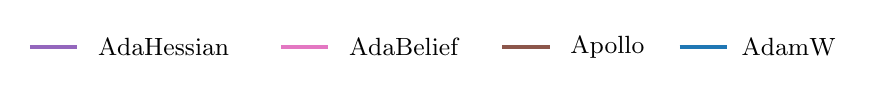
\begin{tikzpicture}[scale=0.75] % Nested TikZ environment
        \small 
        % AdaBelief
        % Adam
        
        \draw[orchid227119194,  ultra thick] (4.25,0) -- ++(0.8,0);
        \node[anchor=west] at (5.25,0) {{AdaBelief}}; % Increased spacing
        
        % AdaHessian
        \draw[sienna1408675,  ultra thick] (8,0) -- ++(0.8,0);
        \node[anchor=west] at (9,0) {{Apollo}}; % Increased spacing
        
        % Apollo
        \draw[steelblue31119180,  ultra thick] (11,0) -- ++(0.8,0);
        \node[anchor=west] at (11.9,0) {{AdamW}}; % Increased spacing
        
        \draw[mediumpurple148103189,  ultra thick] (0,0) -- ++(0.8,0);
        \node[anchor=west] at (1,0) {{AdaHessian}}; % Increased spacing
        
\end{tikzpicture}
};
    \end{tikzpicture}
     \\ % Replace with the correct path to your .tex file
        
    \end{tabular}
    \caption{Evaluation of optimizers on WMT-14 using the Transformer architecture with the \texttt{InverseSquareRootLR} learning rate scheduler.
    Hyperparameters are individually tuned for optimal performance.}
    \label{fig:wmt14-perf-opt}
\end{figure}

\begin{table}[h!]
    \centering
    \caption{Cost, Speed, and Memory Usage of Different Optimizers Across Various Datasets}
    \label{tab:optimizer_comparison_perf}
    \begin{tabular}{lcccccccccccc}
        \toprule
        & \multicolumn{2}{c}{CIFAR-10} & \multicolumn{2}{c}{Tiny ImageNet}  & \multicolumn{2}{c}{WMT-14} \\
        \cmidrule(lr){2-3} \cmidrule(lr){4-5}  \cmidrule(lr){6-7} 
        Cost (x SGD) & Speed & Memory  & Speed & Memory  & Speed & Memory  \\
        \midrule
        SGD         & 1.0 & 1.0 & 1.00 & 1.00 & 1.00 & 1.00  \\
        Adam        & 1.0292 & 1.0112 & 1.0502 & 1.2192& 1.0217 & 1.02174 \\
        AdamW       & 1.0317 & 1.0112 & 1.0458& 1.2151 &  1.0299 & 1.02993 \\
        AdaBelief   & 1.0402 & 1.0112 & 1.0581 & 1.2273 & 1.0389 & 1.03895 \\
        RMSProp     & 1.0213 & 1.0 & 1.0274 & 1.0079 & - & - \\
        Apollo      & 1.1337 & 1.0223 & 1.1616 & 1.4313 & 1.1167 & 1.11669  \\
        ApolloW     & 1.1359 & 1.0223 & 1.1556 & 1.4336 & 1.1183& 1.11828   \\
        AdaHessian  & \textbf{2.6654} &\textbf{3.6443}& \textbf{1.9098}  & \textbf{2.7969} & \textbf{2.6121} &\textbf{1.716}\\
        \bottomrule
    \end{tabular}
\end{table}




